\RequirePackage[l2tabu]{nag}		% Warns for incorrect (obsolete) LaTeX usage

% --- Style file for Latex
% In this template package, it can be found in ./Class/
\documentclass{Latex/Classes/GenThesis}

% Adding metadata:
\usepackage{changepage}
\usepackage{datetime}

% --- Macro file for Latex
% Macros help you summarise frequently repeated Latex commands.P
% Here, they are placed in an external file /Latex/Macros/MacroFile1.tex
% An macro that you may use frequently is the figuremacro (see introduction.tex)
% This file contains macros that can be called up from connected TeX files
% It helps to summarise repeated code, e.g. figure insertion (see below).

% insert a centered figure with caption and description
% parameters 1:filename, 2:title, 3:description and label
\newcommand{\figuremacro}[3]{
	\begin{figure}[htbp]
		\centering
		\includegraphics[width=1\textwidth]{#1}
		\caption[#2]{\textbf{#2} - #3}
		\label{#1}
	\end{figure}
}

% insert a centered figure with caption and description AND WIDTH
% parameters 1:filename, 2:title, 3:description and label, 4: textwidth
% textwidth 1 means as text, 0.5 means half the width of the text
\newcommand{\figuremacroW}[4]{
	\begin{figure}[htbp]
		\centering
		\includegraphics[width=#4\textwidth]{#1}
		\caption[#2]{\textbf{#2} - #3}
		\label{#1}
	\end{figure}
}

% inserts a figure with wrapped around text; only suitable for NARROW figs
% o is for outside on a double paged document; others: l, r, i(inside)
% text and figure will each be half of the document width
% note: long captions often crash with adjacent content; take care
% in general: above 2 macro produce more reliable layout
\newcommand{\figuremacroN}[3]{
	\begin{wrapfigure}{o}{0.5\textwidth}
		\centering
		\includegraphics[width=0.48\textwidth]{#1}
		\caption[#2]{{\small\textbf{#2} - #3}}
		\label{#1}
	\end{wrapfigure}
}

% predefined commands by Harish
\newcommand{\PdfPsText}[2]{
  \ifpdf
     #1
  \else
     #2
  \fi
}

\newcommand{\IncludeGraphicsH}[3]{
  \PdfPsText{\includegraphics[height=#2]{#1}}{\includegraphics[bb = #3, height=#2]{#1}}
}

\newcommand{\IncludeGraphicsW}[3]{
  \PdfPsText{\includegraphics[width=#2]{#1}}{\includegraphics[bb = #3, width=#2]{#1}}
}

\newcommand{\InsertFig}[3]{
  \begin{figure}[!htbp]
    \begin{center}
      \leavevmode
      #1
      \caption{#2}
      \label{#3}
    \end{center}
  \end{figure}
}


%----- NEWCOMMANDS ELIA ----------------------------

\newcommand{\sref}[1]{Sec.~\ref{#1}}
\newcommand{\fref}[1]{Fig.~\ref{#1}}
\newcommand{\aref}[1]{Appendix~\ref{#1}}
\newcommand{\figwidth}{0.9\columnwidth}

\newcommand{\argc}[1]{\left[#1\right]}
\newcommand{\arga}[1]{\left\lbrace #1\right\rbrace }
\newcommand{\argp}[1]{\left(#1\right)}
\newcommand{\valabs}[1]{\vert #1\vert}
\newcommand{\moy}[1]{\left\langle  #1 \right\rangle }
\newcommand{\moydes}[1]{\overline{#1}}

\newcommand{\Wbar}{ \mathclap{\phantom{W}\overline{\phantom{I}}} W}
\newcommand{\dbar}{d\mkern-6mu\mathchar'26 \!}
\newcommand{\deltabar}{\delta \mkern-8mu\mathchar'26}
\newcommand{\sigc}[1]{\argc{\sigma}(#1)}
\newcommand{\tho}{{\text{\thorn}} }

\newcommand{\gdD}{\mathcal{D}}
\newcommand{\gdO}{\mathcal{O}}
\newcommand{\gdH}{\mathcal{H}}
\newcommand{\gdR}{\mathbb{R}}
\newcommand{\gdC}{\mathbb{C}}
\newcommand{\gdN}{\mathbb{N}}
\newcommand{\gdF}{\mathcal{F}}


\newcommand{\gdHel}{\gdH_{\text{el}}}
\newcommand{\gdHdis}{\gdH_{\text{dis}}}
\newcommand{\gdHtil}{\widetilde{\mathcal{H}}}
\newcommand{\gdHelt}{\widetilde{\gdH}_{\text{el}}}
\newcommand{\gdHdist}{\widetilde{\gdH}_{\text{dis}}}


%---------------------------------
% For the personal comments
%\newcommand{\commperso}[1]{\textcolor{magenta}{#1}}
%\newcommand{\reftoput}[1]{\textcolor{cyan}{#1}}
\newcommand{\commperso}[1]{\textcolor{black}{#1}}
\newcommand{\reftoput}[1]{\textcolor{black}{#1}}

%\newcommand{\meevid}[1]{\textcolor{NavyBlue}{#1}}
\newcommand{\meevid}[1]{\textcolor{black}{#1}}
%\newcommand{\meevidbf}[1]{\textbf{#1}}
\newcommand{\meevidbf}[1]{#1}


\newcommand{\codecouleurperso}{
	\textcolor{Emerald}{Emerald}
	\textcolor{PineGreen}{PineGreen}
	\textcolor{BlueViolet}{BlueViolet}
	\textcolor{DarkOrchid}{DarkOrchid}
	\textcolor{NavyBlue}{NavyBlue}
	\textcolor{MidnightBlue}{MidnightBlue}
	\textcolor{OrangeRed}{OrangeRed}
	\textcolor{RoyalBlue}{RoyalBlue}
	\textcolor{RoyalPurple}{RoyalPurple}
	\textcolor{TealBlue}{TealBlue}	
	\textcolor{Violet}{Violet}	
	\textcolor{RubineRed}{RubineRed}	
	\textcolor{RedViolet}{RedViolet}	
	\textcolor{VioletRed}{VioletRed}	
	\textcolor{Periwinkle}{Periwinkle}	
}
% Emerald, PineGreen, BlueViolet, DarkOrchid, NavyBlue, MidnightBlue, OrangeRed, RoyalBlue, RoyalPurple, TealBlue, Violet, RubineRed, RedViolet, VioletRed, Periwinkle


%---------------------------------


\newcommand{\footnoteremember}[2]{
  \footnote{#2}
  \newcounter{#1}
  \setcounter{#1}{\value{footnote}}
}
\newcommand{\footnoterecall}[1]{
  \footnotemark[\value{#1}]
}



%%% Local Variables: 
%%% mode: latex
%%% TeX-master: "~/Documents/LaTeX/CUEDThesisPSnPDF/thesis"
%%% End: 


% ----------------------------------------------------------------------

% turn off those nasty overfull and underfull hboxes
\hbadness=10000
\hfuzz=50pt

% --------------------------------------------------------------
%               PAGE GEOMETRY AND CHAPTER STYLE
% --------------------------------------------------------------
% Notes:
% - Chapter style can bte modified using the fncychap package. The available styles are
%   listed in the comments. If you don't like any of the styles just comment the line
\usepackage[Sonny]{fncychap}        % Sonny, Lenny, Glenn, Conny, Rejne and Bjarne
\usepackage{epigraph}
\usepackage{graphicx}
\usepackage{subfigmat}
\usepackage{cleveref}
\usepackage{booktabs}
\usepackage{adjustbox}
\usepackage{amsmath}
\usepackage{amsfonts}
\usepackage{amsthm}
\usepackage{bm}
\usepackage{amssymb}
\usepackage[super]{nth}
\usepackage{mathtools}
\usepackage[separate-uncertainty=true]{siunitx}
\usepackage[bottom]{footmisc}
\usepackage[section]{placeins}
\usepackage{tabularx}
\usepackage{comment}
\usepackage{multirow}
\usepackage{booktabs}
\usepackage{afterpage}
\usepackage{bookmark}
\usepackage[titletoc]{appendix}
\usepackage[figuresright]{rotating}
\usepackage{lipsum}
\usepackage{array}
%\sisetup{round-mode=places,round-precision=4}
%\sisetup{[round-mode=figures,round-precision=3]S[round-mode=places,round-precision=2]l}
	
\usepackage{definitions} %% DEFINITIONS
\usepackage{quoting,xparse}
%\usepackage{caption}
%\usepackage{subcaption}
 \addtolength{\textheight}{0.0cm}  % add/remove size to vertical text space in the page
 \addtolength{\voffset}{-0.0cm}    % vertical offset from top AND bottom of the page
 \addtolength{\textwidth}{0.48cm}  % add/remove size to the width of the text in the page
 \addtolength{\hoffset}{0 cm}   % horizontal offset from left AND right edges of the page
 \addtolength{\oddsidemargin}{-0.0cm}   % border size on the odd pages (for bindings)
 \addtolength{\evensidemargin}{0.0cm}   % border size on the even pages (for bindings)
%\newcommand{\Neq}{\ensuremath{\,\rm{n}_{\rm{eq}}/cm^2}}

\NewDocumentCommand{\bywhom}{m}{% the Bourbaki trick
	{\nobreak\hfill\penalty50\hskip1em\null\nobreak
		\hfill\mbox{\normalfont(#1)}%
		\parfillskip=0pt \finalhyphendemerits=0 \par}%
}

\NewDocumentEnvironment{pquotation}{m}
{\begin{quoting}[
		indentfirst=false,
		leftmargin=4cm,
		rightmargin=\parindent]\itshape}
	{\bywhom{#1}\end{quoting}}
\newcolumntype{P}[1]{>{\centering\arraybackslash}p{#1}}
% --------------------------------------------------------------
%                   FRONT MATTER: dedications, abstract,..
% --------------------------------------------------------------
\begin{document}

%\language{english}
% sets line spacing
%\renewcommand\baselinestretch{1.2}
%\baselineskip=18pt plus1pt


% ----------------------- FRONT PAGE ----------------------------------
\fancyend
%\pagenumbering{roman}
% --------------------- FRONT MATTER ----------------------------------

% File: Title.tex
\begin{adjustwidth*}{\unitlength}{-\unitlength}
	\begin{center}
		
\includegraphics[scale=1]{frontmatter/figures/uniroma2}\\
		\vspace{1cm}
		{\large\textsc{DOTTORATO DI RICERCA IN FISICA}}\\
		\vspace{0.8cm}
		{\large\textsc{CICLO DEL CORSO DI DOTTORATO XXXIII}}\\
		\vspace{1cm}
		{\LARGE{Search for the FCNC decay of top-quark in c-quark and Z boson using the ATLAS detector}}\\
		%{\LARGE{Search for the FCNC decay \boldsymbol{$t\rightarrow c + Z$ }\\ using the ATLAS detector}}\\
		\vspace{6.5mm}
		{\large\textsc{Lorenzo Marcoccia}}\\
		\vspace{1cm}
		{\large\textsc{A.A. 2020/2021}}\\
		\vspace{10mm}
		{\large{\textsc{Docente Guida:}  Prof. LUCIO CERRITO}}\\ 
		\vspace{5mm}
		{\large{\textsc{Coordinatore:   }  Prof. ROBERTO BENZI}}\\ 
		\vspace{3mm}
		\begin{minipage}{10cm}
			\vspace{1cm}
			A dissertation submitted to the University of Rome Tor Vergata  in accordance with the requirements of the degree of \textsc{Doctor of Philosophy} in the Faculty of Physics.
		\end{minipage}\\
		\vspace{9mm}
		{\large\textsc{32 November 2184}}
		\vspace{12mm}
	\end{center}
\end{adjustwidth*}

\thispagestyle{empty}
\newpage

% --------------------- QUOTES----------------------------------
\vspace*{3cm} 

\begin{pquotation}{Karl Popper, The Logic of Scientific Discovery}
	`The wrong view of science\\
	 betrays itself in the craving to be right;\\ 
	for it is not his possession of knowledge,\\ 
	of irrefutable truth, that makes the man of science, \\
	but his persistent and recklessly critical quest for truth.'\\
	\newline
\end{pquotation}

% --------------------- ACKNOWLEDGEMENT----------------------------------
%% Thesis Dedictation ---------------------------------------------------

\begin{dedication} %this creates the heading for the dedication page

Dedicace.

\end{dedication}

% ----------------------------------------------------------------------

\fancyend
% Thesis Acknowledgements ------------------------------------------------



%\begin{acknowledgementslong} %uncommenting this line, gives a different acknowledgements heading
\chapter*{Ringraziamenti}

Ci sono tantissime persone che vorrei ringraziare, ma 
sicuramente il primo è il mio \\Prof. Lucio Cerrito, il mio supervisore in questo 
percorso di tre anni nella ricerca in fisica delle particelle elementari.
Il suo continuo supporto ed il costante stimolo durante il Ph.D sono solamente due 
esempi di come un fisico delle particelle dovrebbe essere.
Grazie anche per avermi dato l'opportunità di stare al CERN per un lungo periodo, una bellissima esperienza grazie alla quale ho acquisito molte importanti competenze e conoscenze.\\

\noindent Vorrei estendere i miei ringraziamenti alla Dott.ssa Lidia Dell'Asta, non solo
un membro del gruppo NPTEV ma un'amica, per la
sua supervisione e guida, soprattutto nei momenti più difficili, sempre pronta ad aiutarmi ogni volta e per qualsiasi cosa avessi bisogno. Grazie per aver condiviso con me le tue conoscenze e la tua esperienza.\\

\noindent Un immenso grazie al Dott. Umberto De Sanctis per i numerosi
consigli ed osservazioni, sono stati fondamentali.\\
Umberto è stato un pilastro per me e per tutto il gruppo, è stato un modello, ed un amico.\\

\noindent Un grande abbraccio a tutti gli altri colleghi ed amici del gruppo NPTEV, Marco, Michele, 
Francesco, Maurizio, Adele, Salvatore e Simone. \\
Ognuno di loro ha contribuito alla mia crescita professionale, ma
anche alla creazione di un gruppo di lavoro eccezionale.\\  

\noindent Infine, i miei ringraziamenti speciali vanno ad Elena ed alla mia famiglia, ai quali
dedico la mia tesi.

\setcounter{page}{1}
\pagenumbering{roman}
% We might thank the financements...


% ------------------------------------------------------------------------



\fancyend
%\setcounter{page}{1}

% ----------------------- ABSTRACT ------------------------------------
\small
\phantomsection
\addcontentsline{toc}{chapter}{Abstract}

% Thesis Abstract -----------------------------------------------------
%\begin{abstractslong}   % uncommenting this line, gives a different abstract heading
\chapter*{Abstract}        % this creates the heading for the abstract page

\selectlanguage{english}

Blablabla.

%\end{abstractlongs}



% Thesis Acknowledgements ------------------------------------------------

\chapter*{Personal contributions}         %this creates the heading for the acknowlegments

\selectlanguage{english}

The candidate is smart

% We might thank the financements...



\fancyend

% ----------------------- TABLE OF CONTENTS ---------------------------
\small
\phantomsection
\addcontentsline{toc}{chapter}{Contents}
% levels are: 0 - chapter, 1 - section, 2 - subsection, 3 - subsection
\setcounter{secnumdepth}{3} % organisational level that receives a numbers
\setcounter{tocdepth}{2}    % print table of ts for level 3
\tableofcontents            % print the table of contents
\fancyend

% ----------------------- list of figures/tables ------------------------

%\listoffigures	 % print list of figures
%\listoftables  % print list of tables


% ----------------------- glossary ------------------------

% Tie in external source file for definitions: /0_frontmatter/glossary.tex
% Glossary entries can also be defined in the main text. See glossary.tex
% % this file is called up by thesis.tex
% content in this file will be fed into the main document

% Glossary entries are defined with the command \nomenclature{1}{2}
% 1 = Entry name, e.g. abbreviation; 2 = Explanation
% You can place all explanations in this separate file or declare them in the middle of the text. Either way they will be collected in the glossary.

% required to print nomenclature name to page header
\markboth{\MakeUppercase{\nomname}}{\MakeUppercase{\nomname}}


% ----------------------- contents from here ------------------------

% chemicals
\nomenclature{DAPI}{4',6-diamidino-2-phenylindole; a fluorescent stain that binds strongly to DNA and serves to marks the nucleus in fluorescence microscopy} 
\nomenclature{DEPC}{diethyl-pyro-carbonate; used to remove RNA-degrading enzymes (RNAases) from water and laboratory utensils}
\nomenclature{DMSO}{dimethyl sulfoxide; organic solvent, readily passes through skin, cryoprotectant in cell culture}
\nomenclature{EDTA}{Ethylene-diamine-tetraacetic acid; a chelating (two-pronged) molecule used to sequester most divalent (or trivalent) metal ions, such as calcium (Ca$^{2+}$) and magnesium (Mg$^{2+}$), copper (Cu$^{2+}$), or iron (Fe$^{2+}$ / Fe$^{3+}$)}



 

%\begin{multicols}{2} % \begin{multicols}{#columns}[header text][space]
%\begin{footnotesize} % scriptsize(7) < footnotesize(8) < small (9) < normal (10)

%\printnomenclature[1.5cm] % [] = distance between entry and description
%\label{nom} % target name for links to glossary

%\end{footnotesize}
%\end{multicols}


% --------------------------------------------------------------
%                  MAIN DOCUMENT SECTION
% --------------------------------------------------------------
% the main text starts here with the introduction, 1st chapter,...
\mainmatter
%\renewcommand{\chaptername}{} % uncomment to print only "1" not "Chapter 1"
\setcounter{page}{1}
% ----------------------- subdocuments ------------------------

% Parts of the thesis are included below. Rename the files as required.
% But take care that the paths match.
\small
\selectlanguage{english}
\cleardoublepage
\phantomsection
\addcontentsline{toc}{chapter}{Introduction}
\include{Chapters/CH0/Introduction}

% this file is called up by thesis.tex
% content in this file will be fed into the main document

% ----------------------- introduction file header -----------------------
\chapter{The theory framework}
\label{chapter:SM}
% ----------------------- paths to graphics ------------------------

% the code below specifies where the figures are stored
\graphicspath{Chapters/CH1/figures}
% -----------

The construction of the Standard Model is the result of a long series of experiments
and brilliant ideas in both theoretical and experimental fields.
Towards the end of the 1960s, knowledge of what we consider to be the constituent
elements of nature and the fundamental interactions among them, was organized
in the so-called Standard Model (SM).\\
More recently, a missing piece towards the completion of the SM, the Higgs boson,
was discovered by the ATLAS and CMS collaborations.\\
The ambition is to find a theoretical representation of all phenomena experimentally accessible.\\
Since particle physics is characterized by phenomena that are both relativistic
than quantistic, the description of the Standard Model relies on the
formalism of \textit{Quantum Field Theories} (QFT), synthesis of quantum mechanical
and relativistic theory. In these terms, the concept of field is associated
both to material particles and to forces. Particles are mere manifestations of
fields: they are identified with the quanta of the material fields and
force fields and the interaction among particles is determined by the exchange of virtual quanta of the field.\\
To search for extensions of the SM, it is possible to postulate a scale of the new physics high enough to manifest itself through deviations of known observables, usually at high energies.\\
In this chapter, a concise description of the SM will be presented, from the gauge
principle to the description of several theories of physics beyond the Standard Model which are crucial for the search of FCNC decay of the top quark.

% ----------------------------------------------------------------------
% ----------------------- introduction content -------------------------
% ----------------------------------------------------------------------


\section{The gauge principle in quantum field theory}

The mathematical framework of the SM is based on a quantum field theory description of the particles and their interactions.
The structure is a consequence of the invariance of physics under certain general symmetries:
these invariances are called \textit{gauge} because there is freedom in the choice of a certain number of parameters
that can precisely "calibrate" the model.
Each symmetry is therefore associated with a set of transformations that frame the "gauge group of the theory".
The theory is introduced starting from the Lagrangian formalism developed in the classical mechanism, extending this formalism to
classical field theory and finally to quantum field theory.
\vspace{\baselineskip}
 \\Lagrangian is defined as the difference between the kinetic energy and the potential energy of the system, as below:
\begin{equation}
\mathcal{L} (q,\dot{q}) =  \frac{m}{2}(\dot{q})^2-V(q)
\end{equation}
where $q$ is a set of generalized coordinates and $m$ is the mass of the particle.\\
The \textit{action} is defined as $ S = \int dt \mathcal{L} (q,\dot{q}) $.
\vspace{\baselineskip}
\\Using a variational approach it can be shown that for any possible variation of the path of the particle, $\partial(q)$,
the equation of motion of the system is  the one that minimizes the \textit{action}.
The results are the so called \textit{Euler-Lagrange} equations:
\begin{equation}
	\frac{\partial\mathcal{L}}{\partial q} -  \frac{d}{dt}\bigg(\frac{\partial\mathcal{L}}{\partial\dot{q}}\bigg)=0
\end{equation}
The next step is the extension of the classical mechanics formalism  to field theory. One possible way is to generalize 
the path of a particle which is a function of time $q(t)$, into a function of space-time coordinates $\phi(x)$ which is the
vectorial (or tensorial) representation of the field with Lorentz invariance properties of the space-time.\\
The sub-set of dimension-four vectorial representations used in particle physics is called spinors and they can be decomposed into
left-handed and right-handed components, depending on their chirality: $\psi_{L}$ and $\psi_{R}$. The usual representation for Lorentz and 
parity transformations is the \textit{Dirac} spinor $\Psi = (\psi_{L},\psi_{R}$), which allows describing properly the dynamics of relativistic particles.
\vspace{\baselineskip}
\\At this point, the Lorentz-invariant Lagrangian is the following:
\begin{equation}
	\mathcal{L}_D  =  \bar{\Psi}(i\gamma^{\mu}\partial_{\mu}-m)\Psi
\end{equation}
where $\gamma$ are an extension of the Pauli matrices into a four dimension space and they are called Dirac matrices.
\vspace{\baselineskip}
\\The QFT is also built on the \textit{Noether}’s theorem that relates symmetries of the system to conserved observables.\\
Through this theorem, symmetries become a fundamental building block of the physical theory. 
A particular set of transformations, called gauge transformations, which by construction leave invariant the Lagrangian of the SM, 
constitute a building principle of the SM itself. 
\vspace{\baselineskip}
\\Let us now consider the global $U(1)$\footnotemark \footnotetext{U(1) is the one-dimensional unitary group, i.e. any of its elements can be expressed as a $1\times 1$ matrix whose inverse is equal to its transpose conjugate ($U^{-1}= \bar{U}^*$).}
transformation of the form: 
\begin{equation}
	\Psi \rightarrow e^{i\theta}\Psi
\end{equation}
It can be easily demonstrated that $\mathcal{L}_D$ is invariant under such a transformation and the related conserved observable is
the current $\bar{\Psi}\gamma^{\mu}\Psi$. \\
However, the Lagrangian is no longer invariant under the transformation: $\theta\rightarrow\theta (x)$ which means that the gauge 
invariance is required in each point of the space-time.
\\The inclusion of an additional field, the photon, which mediates the forces, makes the Lagrangian explicitly invariant and it allows
to choose a \textit{gauge} of the theory, in fact the action of free electromagnetic field is invariant under $A_{\mu}\rightarrow A_{\mu}-\partial_{\mu}\theta$,
with $A_{\mu}$ being the four-vector of the electrostatic and magnetic potential: $(V,\vec{A})$.
\vspace{\baselineskip}
\\The above example is useful to understand how the SM is constructed. It is a gauge theory which, analogously to what described in
this section, is invariant under:
\begin{equation} 
	SU(3)_{c} \otimes SU(2)_{L} \otimes U(1)_{Y}
\end{equation}
The $SU(3)_{c}$ describes the strong force (see next section) while $SU(2)_{L} \otimes U(1)_{Y}$ term describes the electro-weak sector (see Section \ref{sec:ew}). 
A more detailed discussions follows.

\subsection{Quantum Chromodynamics} 

The strong interaction between quark and gluons is described by the \textit{Quantum Chromodynamics} (QCD). It is a gauge theory based on non-abelian 
$SU(3)_{c}$\footnotemark \footnotetext{S stands for "special", meaning that the group matrices have determinant 1. C stands for "colour", which is the conserved quantity associated with the symmetry}
and associated to the three colour charges (red, green and blue). A total number of 8 generators $T^a$ of the group, also called Gell-Mann matrices,
represent bosons mediating the force, called \textit{gluons}. They are massless, in contrast with the weak mediators.
\vspace{\baselineskip}
\\The QCD Lagrangian, can be expressed as:
\begin{equation}
\mathcal{L}_{QCD}  =  \bar{\psi}(i\gamma^{\mu}D_{\mu}-m)\psi-\frac{1}{4}G^{a}_{\mu\nu}G^{\mu\nu}_a
\end{equation}
where the index $a$ represent the 8 $SU(3)_C$ generators,  $\frac{1}{4}G^{a}_{\mu\nu}G^{\mu\nu}_a$ is the kinetic term of the gluons ($G^a$ is the gluon field strength tensor) and the covariant derivative $D_{\mu}$ is defined as
\begin{equation}
D_{\mu}=\partial_{\mu}-ig_{s}T_{a}G^{a}_{\mu}
\end{equation}
\vspace{\baselineskip}
\\The coupling constant $\alpha_{s}$ ($\frac{g^2_s}{4\pi}\sim 1)$, is dependent on the transferred momentum $Q^2$ that corresponds to a dependence on the separation between quarks:
\begin{equation}
\alpha_{s}(Q^2)= \frac{33-2n_f}{12\pi}   \ln\left( \frac{Q^2}{\Lambda^{2}_{QCD}}   \right)
\end{equation}
where $n_f$ is the number of quark flavours and $\Lambda^{2}_{QCD}$ is the QCD scale parameter, measured to be $\sim$ 200 \MeV that sets the scale 
between different regimes of the theory. \\
In fact one can discern two cases:
\[\alpha_{s}(Q^2)\xrightarrow[Q^{2} \gg \Lambda^{2}_{QCD} ]{}0\]
\[\alpha_{s}(Q^2)\xrightarrow[Q^{2} \ll \Lambda^{2}_{QCD} ]{}\infty\]
\\In the first case, the quark coupling is asymptotically cancelled, in the limit $Q^{2}\rightarrow \infty$, quarks can be considered as free particles and this phenomena is called \textit{Asymptotic Freedom}.
On the contrary, when the separation becomes relevant, the coupling is so strong to confine quarks in hadronic  structures and this different phenomena is called \textit{Confinement}
The only bound states that occur are completely antisymmetric in the colour variables (the colour singlets), which is equivalent to saying that the possible compositions of quarks must be "white".\\
Interaction between particles that carry charges of colour, takes place through the exchange of gluons of the octet, therefore, not only between quarks and gluons but also between gluons and gluons. This is a very important difference between QED (\textit{Quantum Electrodynamics}) and QCD. In QED, in fact, photons have no charge and cannot couple with each other.

\subsection{The electro-weak sector}
\label{sec:ew}
The first model of the weak interaction was proposed by Fermi in 1933, who proposed an effective field theory at low energies. According to this theory, 
charged current interactions are approximated by a point-like interaction with a coupling called $G_F$~\cite{fermi,wilson}.
At energies $\mathcal{O}$(100~GeV) the theory breaks and the real propagator of the interaction is the $W^\pm$ boson.\\
In 1957, a famous experiment conducted by Wu~\cite{wu} proved that parity is maximally violated by the charged
weak interaction: it only couples to particles of left-handed chirality (and antiparticles of right-handed chirality). There also exists a neutral weak interaction, which couples both
to left-handed and right-handed particles. \\
This discovery motivated the introduction of the vector-axial (V-A) structure of the Lagrangian of the weak force. \\
The model of the weak interaction was subsequently promoted to a gauge theory by requiring local invariance under symmetries of the $SU(2)$ group, and it was associated
with a conserved quantity called the \textit{weak isospin}.
\vspace{\baselineskip}
\\Each generation of left-handed fermions forms a doublet satisfying $I_{3}= \pm\frac{1}{2}$, while right-handed fermions correspond to singlets of null isospin, as follows:
\begin{equation} 
\chi_{L}=\binom{\nu_l}{l}_L  \qquad l_R
\end{equation}
where $ l= (e,\mu,\tau)$, and a right-handed neutrino singlet is not introduced since there is still no observation of such a particle. A similar representation is given for
quarks where both up ($u$, $s$, $t$) and down-types ($d$, $c$, $b$) have a right-handed component, singlet under $SU(2)_L$.
\vspace{\baselineskip}
\\The transitions between quark doublet members corresponds to $SU(2)$ raising ($\tau^+$) and lowering ($\tau^-$) operators, giving the charge raising and lowering currents~\cite{renton}:
\begin{equation*}
J^{+} \sim \; g(\bar{u} \; d_{c}) = g(\bar{u} \; \bar{d}_{c})\left(\begin{array}{cc}  
																								0 & 1 \\ 
																								0 & 0
																								\end{array} \right)  \binom{u}{d_c} = g (\bar{q} \; \tau^{+}q)  
\end{equation*}
\begin{equation}
J^{-} \sim \; g(\bar{d}_c \; u) = g(\bar{u} \; \bar{d}_{c})\left(\begin{array}{cc}  
																								0 & 0 \\ 
																								1 & 0
																								\end{array} \right)  \binom{u}{d_c} = g (\bar{q} \; \tau^{-}q)  
\end{equation}
where overall numerical factors have been omitted, d-quark is 'Cabibbo-rotated' ($\theta_c\;\sim\; 13\si{\degree}$) and  $g$ is the dimensionless weak coupling constant and quaks.\\
If there exist an appropriate symmetry, based on some underlying gauge theory, then a current involving $\tau_3$ is also expected, since these operators are related via 
the commutation relation $\left[  \tau^{+}, \tau^{-}, \right] = 2\tau_3$. Hence, with such a gauge theory symmetry, one would expect the existence of a neutral current
(identified by the $Z^0$ boson) of the form :
\begin {align}
	\begin{split}
		J^{0} & \sim \; 2g (\bar{q} \; \tau_{3}q)  = g(\bar{u} u- \bar{d}_{c} d_{c}) \\
				& = \; g[ \bar{u} u- \bar{d}_{c} d \cos^{2}\theta_{c}  - \bar{s}_{c} s \sin^{2}\theta_{c} - (\bar{d} s + \bar{s} d) \cos\theta_{c}\sin\theta_{c}  ]
	\end{split}						
\end{align}
The terms $\bar{d} s$ and $\bar{s} d$ correspond to strangeness-changing neutral currents (SCNC), which are heavy suppressed in nature. \\
For example, the decay branching ratio $K^{+}\rightarrow \mu^{+} \nu_{\mu}$ is 63.5\%, whereas that for \\$K^{0}_{L}\rightarrow \mu^{+} \mu^{-}$ is $\sim 10^{-8}$.\\
A mechanism to suppress this unwanted strangeness-changing neutral currents was suggested in 1970 by Glashow, Iliopoulos and Maiani (GIM) and it will be described in the next section.

\subsubsection{GIM mechanism}
\label{sec:gim}
Until the beginning of the 1970s, the only three light quarks u, d and s known at this time could explain the observed hadron spectrum, and the observed weak decays of pions
and kaons were mostly in good agreement with the predictions of the \textit{Cabibbo mechanism}.
Glashow, Iliopoulos and Maiani proposed the existence of a second orthogonal doublet, additional to $\binom{u}{d_c}$,  containing a new quark c (charm) with charge $\frac{2}{3}$, as follows~\cite{gim}:
\begin{equation} 
q' = \binom{c}{s_c} = \binom{c}{-d\sin\theta_{c}+s\cos\theta_c}
\end{equation}
Adding this term gives the total neutral current:
\begin {align}
\begin{split}
	J^{0} & \sim \; 2g (\bar{q} \; \tau_{3}q+ \bar{q}' \; \tau_{3}q')  = g(\bar{u} u + \bar{c}c - \bar{d}_{c} d_{c}- \bar{s}_{c} s_{c}) \\
	& = \; g[ \bar{u} u + \bar{c}c - \bar{d} d  - \bar{s}s ]
\end{split}						
\end{align}
That is, the unwanted terms cancel, leaving a flavour diagonal result.
\vspace{\baselineskip}
\\The GIM mechanism gives also the prediction of the charmed quark, before the $J/\Psi$ discovery occurred in 1974.\\
In the three-quarks picture, and according to the Cabibbo mechanism alone, s $\rightarrow$ d transitions via \textit{Flavour Changing Neutral Current} FCNC processes would be possible at all orders of the perturbation expansion. \\
For example, the process $K^{0}_{L}\rightarrow \mu^{+} \mu^{-}$ FCNC decay could take place, in terms of known quark (u and d-quarks), via the "box-diagram" of Figure~\ref{fig:Kdecay_u}.\\
The calculated rate is larger than what was observed experimentally. 
\vspace{\baselineskip}
\\However, including the diagram of Figure~\ref{fig:Kdecay_c}, the total amplitude is:
\begin{equation} 
\mathcal{M} = \mathcal{M}_{(a)} +\mathcal{M}_{(b)} \;\sim\;f(m_u)g^{4}\cos\theta_{c}\sin\theta_{c} - f(m_c)g^{4}\cos\theta_{c}\sin\theta_{c}
\end{equation}
Thus, the c-quark induces a cancellation, giving a BR compatible with the experiments, but not a total cancellation because $m_{c}\neq m_{u}$. Hence, the prediction on the mass of the
c-quark that in the end is $\sim\; 3$~GeV.
\begin{figure}[h]
	\centering
		\subfigure[]{\label{fig:Kdecay_u}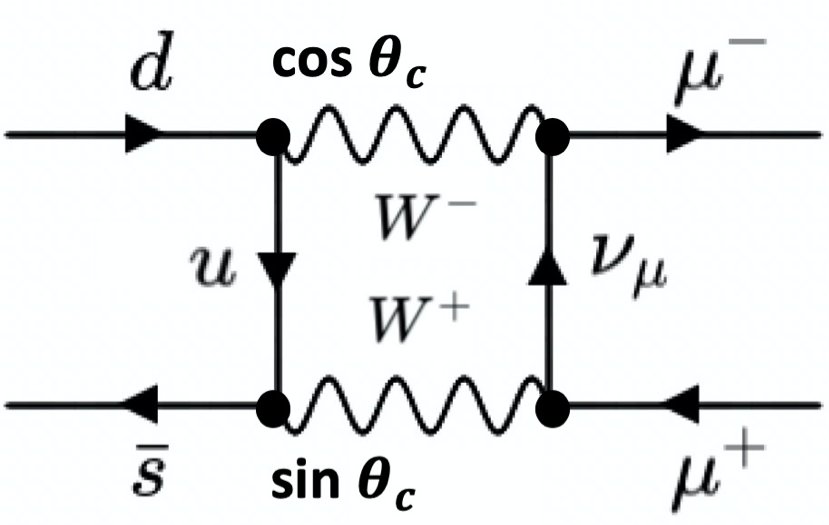
\includegraphics[width=47mm]{Chapters/CH1/figures/kdecay_u}}\qquad
		\subfigure[]{\label{fig:Kdecay_c}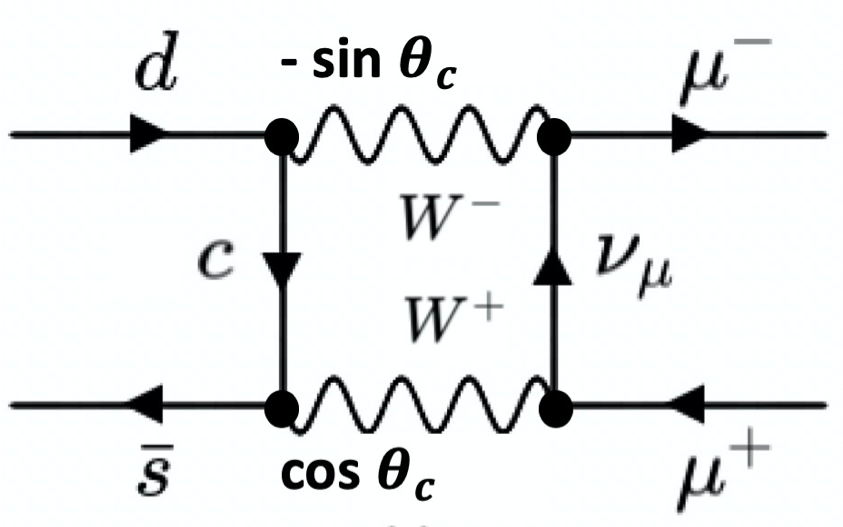
\includegraphics[width=47mm]{Chapters/CH1/figures/kdecay_c}}
	\caption{Feynman diagrams of $K^{0}_{L}\rightarrow \mu^{+} \mu^{-}$ via ($a$) u-quark exchange and ($b$) c-quark exchange}
\end{figure}
In addition to this major prediction, the GIM mechanism led to the prediction that FCNC processes are forbidden at tree-level Leading Order. The branching ratios of several FCNC decays of the top quark in the SM are given in Table~\ref{tab:SM_BR}
\begin{table}[h]
	\begin{adjustbox}{max width=1.\textwidth,center}
		\begin{tabular}{|c|c|c|c|c|c|c|c|c|}
		\hline 
  & $ t\rightarrow uZ$    & $ t\rightarrow cZ$    & $ t\rightarrow u\gamma$ & $ t\rightarrow c\gamma$ & $ t\rightarrow ug$       & $ t\rightarrow cg$       & $ t\rightarrow uH$     & $ t\rightarrow cH$  \\ 
	\hline 
	BR & $8\times 10^{-17} $ & $1\times 10^{-14} $ & $3.7\times 10^{-16} $       & $4.6\times 10^{-14} $      & $3.7\times 10^{-14} $  & $4.6\times 10^{-12} $ & $2\times 10^{-17} $  &$3\times 10^{-15} $  \\ 
		\hline 
		\end{tabular} 
	\end{adjustbox}
\caption{Branching ratios for top quark FCNC interactions in the SM~\cite{aguilar}.}
\label{tab:SM_BR}
\end{table}
\noindent The FCNC production is also sensitive to numerous new physics models, as is mentioned in more details in Section \ref{sec:bsm}.\\
The GIM hypothesis represents a generalization of Cabibbo's idea. The introduction of the fourth quark (c) restored the symmetry
in the (then known)  numbers of quark and leptons.\\
These ideas were extended by Kobayashi and Maskawa (1973), who introduced a framework of six quarks and it will be described in the next section.

\subsubsection{CKM matrix}
\label{sec:ckm}
In 1973 Kobayashi and Maskawa extended the Cabibbo's mechanism allowing to describe the transitions within and in-between 3 generations of quarks
using the so-called \textit{CKM} $3\times3$ matrix~\cite{cabibbo,ckm}, which relates the weak eigenstate of down-type to their mass eigenstate:
\begin{equation}
	\begin{pmatrix}
	d' \\ 
	s' \\ 
	b' 
	\end{pmatrix} 
	= V_{CKM}
	\begin{pmatrix}
	d \\ 
	s \\ 
	b
	\end{pmatrix} 
	=
	\begin{pmatrix}
	|V_{ud}| & |V_{us}| & |V_{ub}| \\ 
	|V_{cd}| & |V_{cs}| & |V_{cb}| \\ 
	|V_{td}| & |V_{ts}|  &| V_{tb}|
	\end{pmatrix} 
	\begin{pmatrix}
	d \\ 
	s \\ 
	b
	\end{pmatrix} 
\end{equation}
By  convention, the up-type quarks are taken to be pure states.
Therefore, partners of the up-type quarks within the weak isospin doublets are the weak eigenstates d’, s’ and b’ which are the pure states. \\
The CKM matrix is fully defined by 4 independent parameters, which must be determined experimentally. These parameters are: 3 mixing angles and 1 CP-mixing
phase, which violates the CP\footnotemark symmetry in the SM~\cite{cp_vio}.
The diagonal elements of the CKM matrix are close to 1, reflecting the fact that transitions are favoured between quarks of the same generation. 
The CKM matrix is unitary, i.e. the sum of the transition probabilities for any quark flavour is equal to 1. If this assumption was to be disproved, 
it could imply the existence of a fourth quark generation.
\footnotetext{Charge transformation followed by a parity transformation.}

%\vspace{1cm}
%\textbf{METTERE Electroweak symmetry breaking ???}
%\clearpage
%\subsection{Electroweak symmetry breaking}  METTERE ???

\section{Top quark physics}
The heaviest known elementary particle described by the Standard Model is the top quark.\\
In 1995, the top quark discovery at FERMILAB~\cite{CDF,D0} was a great success for the SM predictions e.g. the corroboration of existence  of a weak isospin partner of the top quark.
Due to its large mass, the predicted lifetime $\mathrm{\tau_{t} \approx 5\times 10^{−25}}$ s (in agreement with theoretical expectations~\cite{LHcb_top}) entail that it decays before hadronising.\\
In the next sections, the production mechanism is reported, as well as an overview of the decay channels.
\subsection{Production}
The top quark can either be produced as pairs, via strong interaction, or as a single top quark via electroweak interaction that doe not preserve the flavour.\\
The main parton sub-processes that lead to top-pair production are the quark-antiquark annihilation ($q\bar{q}\rightarrow t\bar{t}$, Figure~\ref{fig:top_prod_a}) and the gluon-gluon fusion ($gg\rightarrow t\bar{t}$, \Cref{fig:top_prod_b,fig:top_prod_c}).\\
\begin{figure}[h]
	\centering
	\subfigure[]{\label{fig:top_prod_a}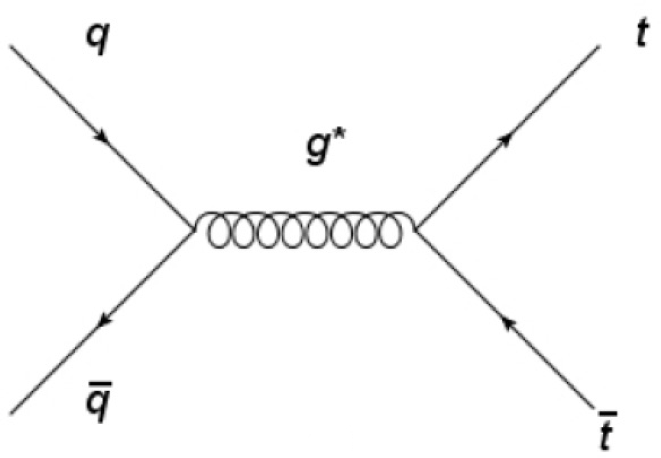
\includegraphics[width=37mm]{Chapters/CH1/figures/top_prod_a}}\quad
	\subfigure[]{\label{fig:top_prod_b}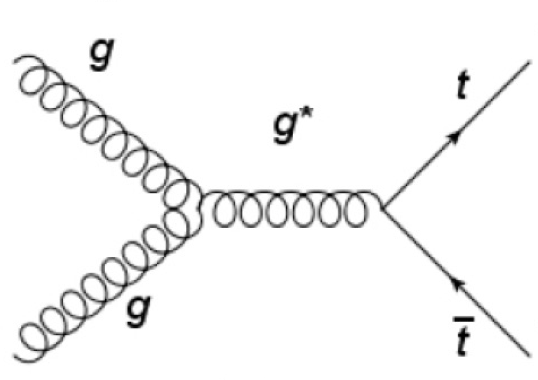
\includegraphics[width=35mm]{Chapters/CH1/figures/top_prod_b}}\quad
	\subfigure[]{\label{fig:top_prod_c}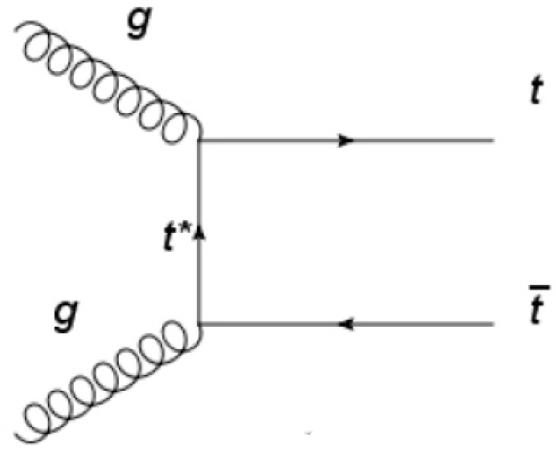
\includegraphics[width=33mm]{Chapters/CH1/figures/top_prod_c}}
	\caption{Feynman diagrams of $t\bar{t}$ production via \subref{fig:top_prod_a} quark-antiquark annihilation ($q\bar{q}\rightarrow t\bar{t}$), \subref{fig:top_prod_b} and \subref{fig:top_prod_c} gluon-gluon fusion ($gg\rightarrow t\bar{t}$) }
\end{figure}
\newline Since in protons there are no valence antiquark, the quark-antiquark annihilation is suppressed by 
the parton distribution functions (PDF) of the antiquark in the proton. Therefore, at the LHC the dominant process turns out to be the
gluon-gluon fusion, while in a proton-antiproton collider, such as Tevatron,
the dominant process is the quark-antiquark annihilation, in fact:
\begin{itemize}
	\item Tevatron: $q\bar{q}\rightarrow t\bar{t} \approx 86\%$, $gg\rightarrow t\bar{t} \approx 15\%$
	\item LHC: $q\bar{q}\rightarrow t\bar{t} \approx 20\%$, $gg\rightarrow t\bar{t} \approx 80\%$
\end{itemize}
Top-pairs can be produced also by the weak interaction when two quarks exchange $Z^0$ or a $\gamma$; however the cross-section of these
type of processes is negligible when compared to the production cross-section through strong interaction.\\
Although at the LHC the top quarks are mainly produced in the process described above, a not negligible number of tops 
are produced singly by weak interaction. The production cross section, in this case, is equal to approximately 1/3 of the top-pair production
cross-section, which is $\sigma_{t\bar{t}} = 831.8^{+19.8+35.1}_{-29.2-35.1}$ pb~\cite{pdg}, at $\sqrt{13}$ TeV and taking into account a top quark mass of 172.5 \GeV.

\subsection{Decay channels}
Since the top quark mass is larger than the W boson mass, the top decays through the weak interaction, mainly in to $t\rightarrow W^{+}b$; according to the SM in 100\% of the possible cases.\\
The other channels ($t\rightarrow W^{+}s$, $t\rightarrow W^{+}d$) are strongly suppressed by the CKM matrix elements (see Section \ref{sec:ckm}). Exploiting the matrix unitarity 
and the B meson oscillation measurements, it is possible to extract the following BRs\cite{tdecayBR}:
\begin{table}[!ht]
	\centering
	\begin{tabular}{l}
		%\hline
		BR$(\mathrm{t \rightarrow W^{+} b)\sim 0.998}$\\
		%\hline
		BR$(\mathrm{t \rightarrow W^{+} s)\sim 1.9\cdot10^{-3}}$\\
		%\hline
		BR$(\mathrm{t \rightarrow W^{+} d)\sim 10^{-4}}$\\
		%\hline
	\end{tabular}
\end{table}
\newline Therefore, the top decay total width is given by, in good approximation, the decay $(t \rightarrow W^{+} b)$, thus equals to $\Gamma_t = 1.44$~GeV.
The W boson may decay in only two ways: "leptonically" \\($W\rightarrow l\nu$) or "hadronically" ($W\rightarrow q\bar{q}'$). This leads to three different categories
of $t\bar{t}$ decays: dileptonic, semi-leptonic or hadronic.\\ Figure~\ref{fig:ttBR} summarizes the BRs associated to each channel.\\
At hadron colliders, the dominant hadronic mode is the most difficult to isolate due to the large QCD background.
\begin{figure}[!h]
	\centering
	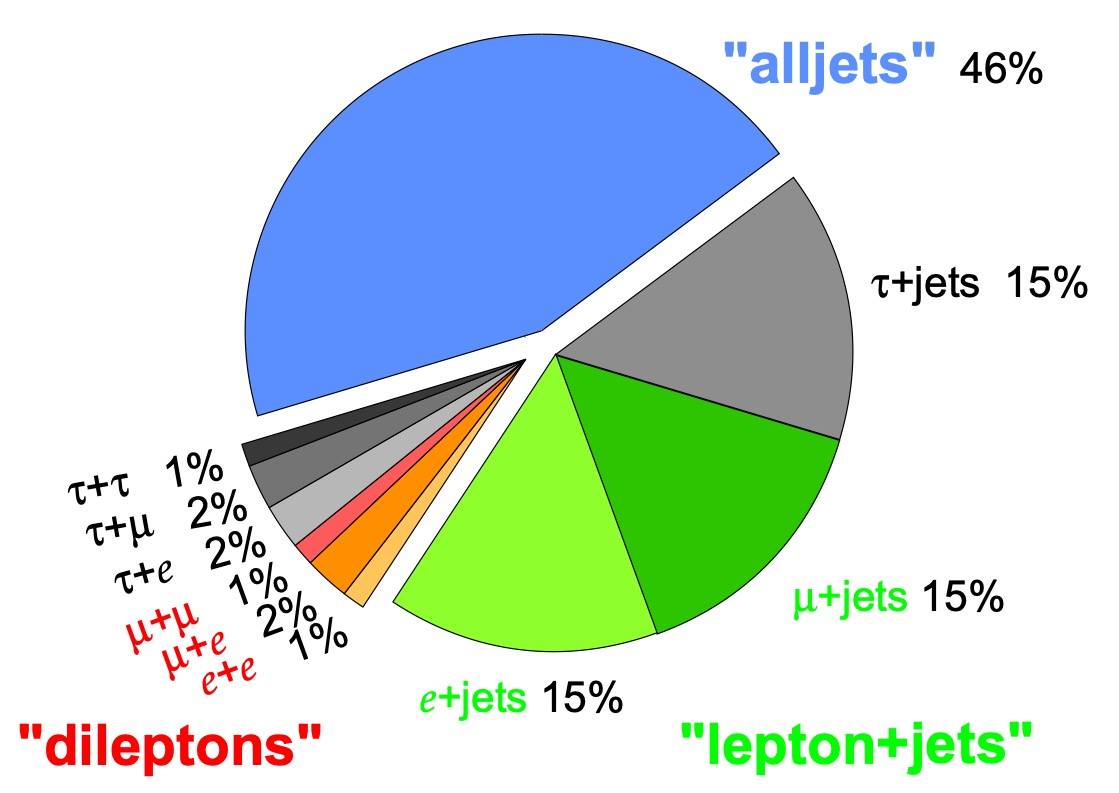
\includegraphics[width=0.55\textwidth]{Chapters/CH1/figures/ttBR}
	\caption{Branching rations associated to each $t\bar{t}$ decay channel \cite{ttdecayBR}.}
	\label{fig:ttBR}
\end{figure}

\newpage
\section{Theories for physics beyond the Standard Model}
\label{sec:bsm}
The previous sections described the core components of what we call \textit{Standard Model} and report few major successes of many. 
Its predictive power makes this model the most tested in physics and it reached the culmination of success on 4 July 2012, when
the ATLAS and CMS experiments at CERN announced the observation a new particle in the mass region around 125~GeV, the
Higgs boson~\cite{higgsDiscovery}. \\
But in spite of its important achievements, the SM falls short of explaining several important observations that in this section
are briefly reported.
\begin{itemize}
\item The SM considers neutrinos as massless particles but this is in contradiction with the results of many experiments, which observed,
in several different contexts, the \textit{neutrino oscillations}. 
It is a quantum mechanical phenomenon whereby a neutrino created with a specific lepton family number ($e$, $\mu$, or $\tau$) 
can later be measured to have a different lepton family number and this mechanism, implies that the neutrino has a non-zero mass 
since it arises from mixing between the flavour and mass eigenstates of neutrinos. 
\item The SM can not describe \textit{dark matter} and \textit{dark energy}. The first evidence of dark matter came with the observation of 
the rotational speed of galaxies, which suggests the existence of a huge amount of undetected mass~\cite{zwicky}.\\
None of the SM particles could explain this phenomenon and, since a dark matter has never been directly observed, implies that
it interacts only weakly with the ordinary matter and radiation, or does not interact at all.\\
Likewise, dark energy is an unknown form of energy that affects the universe on the largest scales.
The first observational evidence for its existence came from supernovae measurements, which showed that the universe does 
not expand at a constant rate; rather, the expansion of the universe is accelerating.\\
The data collected by the Planck spacecraft, indicate that dark energy contributes  68\% of the total energy in the present-day observable universe. 
The mass–energy of dark matter and ordinary (baryonic) matter contributes 27\% and 5\%, respectively, and other components 
such as neutrinos and photons contribute a very small amount~\cite{plank}. 
\item After the Big Bang one could expect that the universe produced the same amount of particles-antiparticles and that the constant annihilation
of pairs would have resulted in a universe of radiation. What we observe actually is large cosmological matter (but not antimatter) structures.
The mechanism suggested by the SM through the CP-symmetry violation of neutral oscillating hadrons is not sufficient to explain alone this phenomenon.
\item There are also other strong indications that the SM could be not yet complete. Indeed, it is based on 19 parameters (excluding neutrino masses)
that must be determined experimentally and have no known theoretical origin.  Moreover, gravity could not be included as a gauge theory because, 
describing graviton (the associated gauge boson) interactions, the classical theory of  Feynman diagrams, and semiclassical corrections with 
at least two loops lead to \textit{ultraviolet divergences}. These infinite results cannot be removed 
because quantized general relativity is not perturbatively renormalizable, unlike QED and models such as the Yang–Mills theory. 
Therefore, when the probability of a particle to emit or absorb gravitons is calculated, the theory loses predictive veracity. 
Those problems and the complementary approximation framework are grounds to show that a theory more unified than quantized general relativity is 
required to describe the behaviour near the Planck scale. 
\item The problem of \textit{naturalness} is also much debated in literature. The Higgs boson is very sensitive to loop corrections and if one considers the theory close to the Planck scale, the corrections involving the top quark may not explain why the Higgs boson mass is so relatively small ($\sim$125 GeV). Another problem is, in fact, the mass scale of fermions that it ranges across many orders of magnitude without any clear explanation.
\end{itemize}
Many are models of "new physics" that attempt to describe and explain the phenomena mentioned above but so far there is no evidence of new physics Beyond Standard Model (BSM). 
In the SM, top quark decays almost exclusively into $bW$ while flavour-changing neutral current (FCNC) decays such as $t\rightarrow qZ$ are forbidden at tree level. 
FCNC decays occur at one-loop level (Figure~\ref{fig:tqZ_fey}) but are strongly suppressed by the GIM mechanism (Section \ref{sec:gim}), with a suppression factor of 14 orders of
magnitude relative to the dominant decay mode\cite{tcZ_sm}.
\begin{figure}[!h]
	\centering
	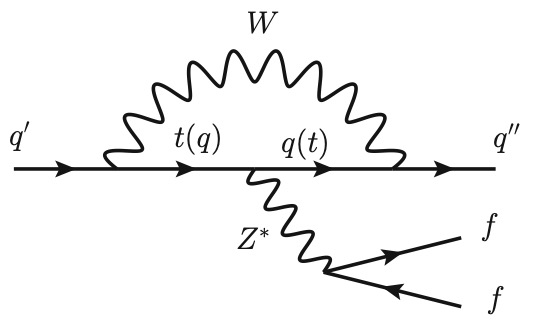
\includegraphics[width=0.5\textwidth]{Chapters/CH1/figures/tqZ_fey}
	\caption{Sketched Feynman diagram for SM $q' \rightarrow q'' f \bar{f}$ induced by the $tqZ$ coupling, where $q'$ and $q''$ denote the down-type quarks; $q = u, c$, and $f$ can be any possible fermions. In the Standard Model, FCNC processes are forbidden at tree level but occur at one-loop level (see GIM mechanism in Section \ref{sec:gim}).}
	\label{fig:tqZ_fey}
\end{figure}

\noindent However, in the BSM models, the suppression could be relaxed and the loop diagrams mediated by new bosons that could contribute, 
leading to couplings of many orders of magnitude higher than those expected by the SM.\\
Examples of such extensions are the quark-singlet model (QS)\cite{qs_limit}, the two-Higgs-doublet model with (FC 2HDM) or without (2HDM) flavour conservation\cite{h2dm_limit},
the Minimal Supersymmetric Standard Model (MSSM)\cite{mssm_limit}, the MSSM with R-parity violation (RPV SUSY)\cite{RPV_limit}, models with warped extra dimensions (RS)\cite{extra_limit}, or extended mirror fermion models (EMF)~\cite{rs_limit}.
Reference~\cite{report_limit} gives a comprehensive review of the various extensions of the SM that have been proposed.
Table~\ref{tab:expBR} provides the maximum values for the branching ratios  predicted by these models and compares them to the value predicted by the SM.\\
In this section we will briefly describe some of these theories interesting for the topics of this thesis.
\begin{table}[!h]
	\begin{adjustbox}{max width=1.\textwidth,center}
		\begin{tabular}{ccccccccc}
			\hline 
			Model:&  			                         SM&  				   QS&  			   2HDM&  				FC 2HDM				& MSSM 			&  RPV SUSY			&  			RS				& EMF \\ 
			\hline 
			$\mathcal{B}(t\rightarrow qZ)$ & $10^{-14}$     & $10^{-4}$ &  $10^{-6}$          & $10^{-10}$  & $10^{-7}$      &$10^{-6}$            & $10^{-5}$           & $10^{-6}$  \\ 
			\hline 
		\end{tabular} 
	\end{adjustbox}
\caption{Maximum allowed FCNC $t\rightarrow qZ$, ($q$ = $u$, $c$) branching ratios predicted by several models\cite{tcZ_sm,qs_limit,h2dm_limit,mssm_limit,RPV_limit,extra_limit,rs_limit,report_limit}.}
\label{tab:expBR}
\end{table} 

\subsection{Quark singlets}
The need to suppress the FCNC mechanism lead to:
\begin{itemize}
	\item they are not mediated by $Z^0$ boson at tree-level
	\item no FCNC mechanism in the scalar sector at tree-level 
\end{itemize}
It is possible to overcome these dogmas using extensions of the SM, like the Quark Singlets (QS)~\cite{barger} that introduces a vector-like quark ($\mathrm{Q=\frac{1}{3}}$ or $\mathrm{Q=\frac{2}{3}}$), thus a small violation of the $\mathrm{3 \times 3}$ $V_{CKM}$ unitarity (see Section \ref{sec:ckm}), mediated by $Z^0$ boson and natural 
FCNC suppression at tree-level.
\vspace{\baselineskip}
\\Given $x_L$ and $x_R$, $SU(2)_{L}$ singlets
\begin{equation}
\begin{pmatrix}
d' \\ 
s' \\ 
b' \\
x' 
\end{pmatrix} 
=
\begin{pmatrix}
|V_{ud}| & |V_{us}| & |V_{ub}|  & |V_{ux}| \\ 
|V_{cd}| & |V_{cs}| & |V_{cb}|   & |V_{cx}| \\ 
|V_{td}| & |V_{ts}|  &| V_{tb}|   & |V_{tx}|
\end{pmatrix} 
\begin{pmatrix}
d \\ 
s \\ 
b \\
x
\end{pmatrix} ,
\end{equation}
the non orthogonality of the columns leads to terms of the type:
\begin{equation}
J_{\mu}= \frac{g}{cos\theta_W}Z_{bd}\bar{b}_{L}\gamma_{\mu}d_{L}Z^{\mu}
\end{equation}
where
\begin{equation}
Z_{bd}=V_{ud}V^*_{ub}+V_{cd}V^*_{cb}+V_{td}V^*_{tb}
\end{equation}
and $Z_{bd}$ is suppressed by $\frac{m_q}{m_x}$.
\vspace{\baselineskip}
\\In this way it is possible to have deviations from $\mathrm{3 \times 3}$ unitarity.\\
For instance, the PMNS matrix in the leptonic sector, in the context of the see-saw mechanism is not  $\mathrm{3 \times 3}$ unitarity~\cite{pnms}.
\\Vector-like quarks provide the simplest model with spontaneous \textit{CP violation} and a framework to have a common origin
of all CP violation, because it is a potential solution of the \textit{strong CP problem}.

\subsection{Two Higgs Doublet Model}
The LHC discovery of a Standard-Model-like Higgs H(125) particle in 2012\cite{higgsDiscovery} could be a portal to an extended Higgs sector predicted by several models. One of such models is the Two-Higgs-Doublet Model (2HDM)~\cite{h2dm}.
The most natural extension of the Standard Model scalar sector is the addition of an
extra $SU(2)_{L}$ doublet. 
\vspace{\baselineskip}
\\The 2HDM is an \textit{Effective Field Theory} (EFT\footnotemark) 
\footnotetext{ An EFT corresponds to a low-energy approximation to
a more fundamental underlying theory, characterized by an energy scale $\Lambda$ (e.g. the mass
of new particles)}
consisting of two complex Higgs doublets, which provide masses to both the up-type and the down-type fermions:
\begin{equation} 
	\Phi_{1}= \binom{\phi^{+}_{1}}{\phi^{0}_{1}}  \qquad \Phi_{2}= \binom{\phi^{+}_{2}}{\phi^{0}_{2}}
\end{equation}
with the minimum of the potential corresponding to
\begin{equation} 
	\Phi_{1,0}= \frac{1}{\sqrt{2}}\binom{0}{\nu_1}  \qquad \Phi_{2,0}= \frac{1}{\sqrt{2}}\binom{0}{\nu_2}.
\end{equation}
\\After the electroweak symmetry breaking (EWSB),
there are five physical scalar fields, consisting of neutral bosons $h,H,A$ of which the
first two bosons are CP-even, as opposed to the A-boson which is CP-odd and of two charged Higgs states $H^{\pm}$.
\\The model is parametrized by the five Higgs masses ($m_H$, $m_h$, $m_{H^{\pm}}$, $m_A$), the ratio of the vacuum expectation 
values of the two Higgs doublets $\tan{\beta}= \nu_{2}/\nu_{1}$ and the mixing angle $\alpha$ between the CP-even Higgs states.
\\There exist four types of 2HDM which simultaneously forbid the presence of FCNC and preserve CP symmetry:
\begin{itemize}
	\item in Type I all fermions couple to the second doublet $\Phi_2$. It follows that BR are independent of $\tan{\beta}$;
	\item in Type II or MSSM-like scenario, lepton and down-type quarks couple to the first doublet $\Phi_1$, whilst up-type quarks couple to $\Phi_2$;
	\item in Type III or lepton specific scenario, quarks couple to  $\Phi_2$ while leptons couple to the other doublet;
	\item in Type IV or flipped model, the coupling of the leptons is reversed with respect to the Type-II model.
\end{itemize}	
	
\subsection{Minimal Supersymmetric Standard Model}
The FCNC processes have also been studied within the \textit{Minimal Supersymmetric Standard Model} (MSSM), where there are loop corrections of the supersymmetric QCD with gluinos 
and scalar quarks, as shown in Figure~\ref{fig:fey_mssm}.
\begin{figure}[!h]
	\centering
	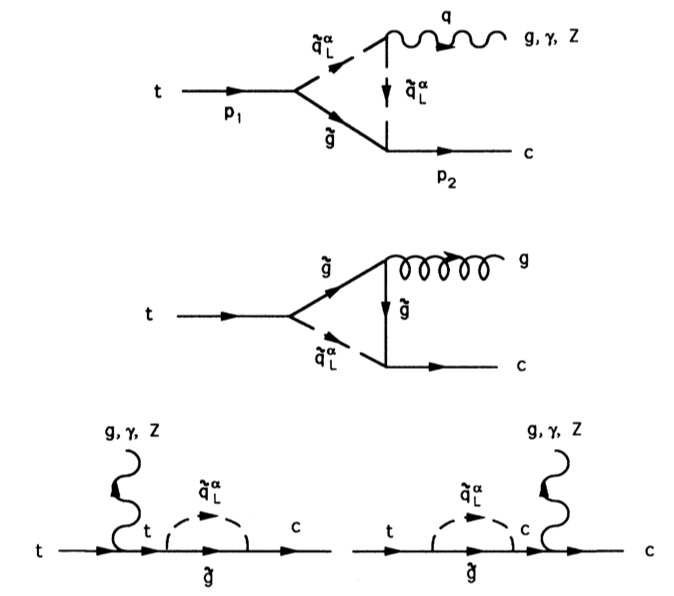
\includegraphics[width=0.55\textwidth]{Chapters/CH1/figures/fey_mssm}
	\caption{The diagrams with scalar quarks and gluinos within the loop, which contribute to the top quark decay into a charm quark and a Z boson, photon, or gluon\cite{coulture_mssm}.}
	\label{fig:fey_mssm}
\end{figure}
In supersymmetric QCD it was shown that there occurs flavour-changing strong interactions between the gluino, the left-handed quarks, and their supersymmetric scalar
partners, whereas the couplings of the gluino to the right-handed quarks and their partners remains flavour diagonal.
To calculate the one-loop diagrams shown in Figure~\ref{fig:fey_mssm}, we need the couplings of the gluon to the gluinos, of the
scalar partners of the left-handed quarks to the gluon, photon, and Z boson, and of the gluino to the left-handed quark and its scalar partner.\\
After the introduction of non-trivial squark mixing, it is possible to calculate the coupling that leads to flavour changing in which appears $K_{ij}$, the supersymmetric version of $V_{CKM}$:
\begin{equation}
\begin{pmatrix}
	1                  & \epsilon   & \epsilon^2 \\ 
	-\epsilon     & 1              & \epsilon \\ 
	-\epsilon^2 & -\epsilon & 1
\end{pmatrix} .
\end{equation}
It is possible to demonstrate that all divergent terms cancel exactly, without the GIM mechanism.\\
Finally, we define $\mathcal{B}(t \rightarrow cZ)=\frac{\Gamma_{S}(t \rightarrow cZ)}{\Gamma_{W}(t \rightarrow bW)}$, where:
\begin{equation} 
\Gamma_{W}(t \rightarrow bW) = \frac{\alpha}{16\sin{\Theta_W}} m_{top} \left(1-\frac{m^{2}_{W}}{m^{2}_{top}}\right)^2 \left(2+\frac{m^{2}_{top}}{m^{2}_{W}}\right)
\end{equation}
Using the following values for the parameters $m_{top}=174$~GeV, $\alpha_{s}=1.4675/\ln{\left( \frac{m^{2}_{top}}{\Lambda^{2}_{QCD}} \right)}$ with $\Lambda_{QCD}=0.18$~GeV, it is
possible to derive the branching ratio $\mathcal{B}(t \rightarrow cZ)$ as a function of the scalar mass $m_{S}$ for a gluino mass of 100~GeV (Figure~\ref{fig:BR_mssm}).
\begin{figure}[!h]
	\centering
	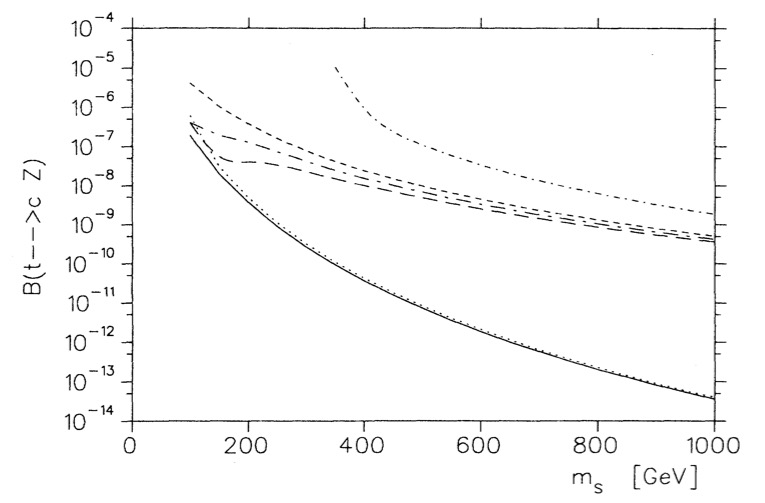
\includegraphics[width=0.65\textwidth]{Chapters/CH1/figures/BR_mssm}
	\caption{The branching ratio $\mathcal{B}(t \rightarrow cZ)$ as a function of the scalar mass $m_{S}$. The gluino mass was taken to be 100~GeV. The solid line is the unphysical case 
		with no squark mixing, the dotted lines are different scenarios of squark mixing\cite{coulture_mssm}.}
	\label{fig:BR_mssm}
\end{figure}
\\We see that without mixing, $\mathcal{B}(t \rightarrow cZ)$ decreases rapidly with increasing scalar mass. The mixing has a drastic effect. It enhances the branching ratio by up to 
5 orders of magnitude for large $m_{S}$.
\clearpage
\let\cleardoublepage\clearpage



% this file is called up by thesis.tex
% content in this file will be fed into the main document

% ----------------------- introduction file header -----------------------
\chapter{The LHC accelerator and the ATLAS experiment}
\label{chapter:ATLAS}
\begin{figure}[!h]
	\centering
	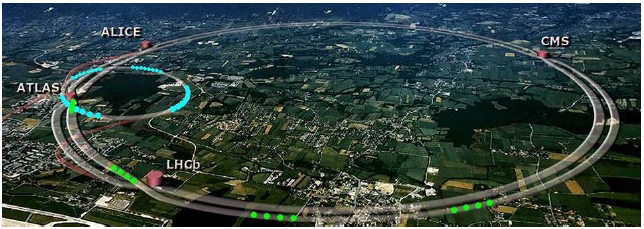
\includegraphics[width=0.885\textwidth]{Chapters/CH2/figures/CERN}
	\caption{The LHC ring, aerial view.}
	\label{fig:CERN}
\end{figure}
\noindent This chapter main focus is the experimental setup, thus the ATLAS detector, one of the four large experiments at CERN (\textit{Conseil Européen pour la Recherche Nucléaire}) and shown in Figure~\ref{fig:CERN}.\\\
Established in 1954, CERN is the largest particle physics laboratory in the world and the organization is based in a north-west suburb of Geneva on the Franco–Swiss border.
The analysis presented in this thesis is based on the data collected in the 2015, 2016, 2017 and 2018.
Since December 2018, LHC has been shut-down (LS2, 2019-2020) to undergo a major upgrade (Phase \MakeUppercase{\romannumeral 1} Upgrade) which may enable to collect up to 300~$\mathrm{fb^{-1}}$ at a c.o.m. energy of 14~TeV until 2023. 
After that, a second major upgrade  (Phase \MakeUppercase{\romannumeral 2} Upgrade) is planned to the LHC (LS3, 2014-2025) which will increase the interaction rate by a factor of 10; this upgrade 
will lead LHC to High-Luminosity LHC (HL-LHC). 
% ----------------------- paths to graphics ------------------------

% the code below specifies where the figures are stored
\graphicspath{Chapters/CH2/figures}

% ----------------------------------------------------------------------
% ----------------------- introduction content -------------------------
% ----------------------------------------------------------------------

\section{The LHC accelerator}
Located at CERN, the Large Hadron Collider (LHC) ~\cite{CERN_acc}. is the world’s highest energy particle accelerator.
LHC is a circular hadron accelerator, positioned at a depth of about 100~m in the tunnel built for the LEP accelerator, at CERN in Geneva.
It is 26.6~km long and currently operates by making proton beams collide at an energy $ \sqrt {s} = $ 13~TeV. \\
CERN's choice to replace the LEP leptonic collider with an hadronic one, such as LHC, has brought two fundamental advantages: the first is that for the same infrastructural size it is possible to reach a higher energy in the center of mass, since the energy lost by radiation of synchrotron from a particle in circular motion is $\frac{dE}{dt}\propto\frac{E^4}{m^4R}$, where $R$ is the bending radius and $m$ is the mass of the accelerated particle travelling at an energy $E$.\\
The second advantage is that the composite structure of the protons allows access to a wider energy spectrum that can be explored simultaneously without having to change the beam parameters. On the other hand, the number of events considered as a background also increases.
In addition to proton-proton (p-p) collisions, at LHC collisions between heavy lead ions (Pb-Pb) also occur . \\
Before reaching the highest possible energy at the LHC, the protons undergo subsequent acceleration steps. The overall accelerator complex is shown in Figure~\ref{fig:CERN_complex}.
\begin{figure}[!h]
	\centering
	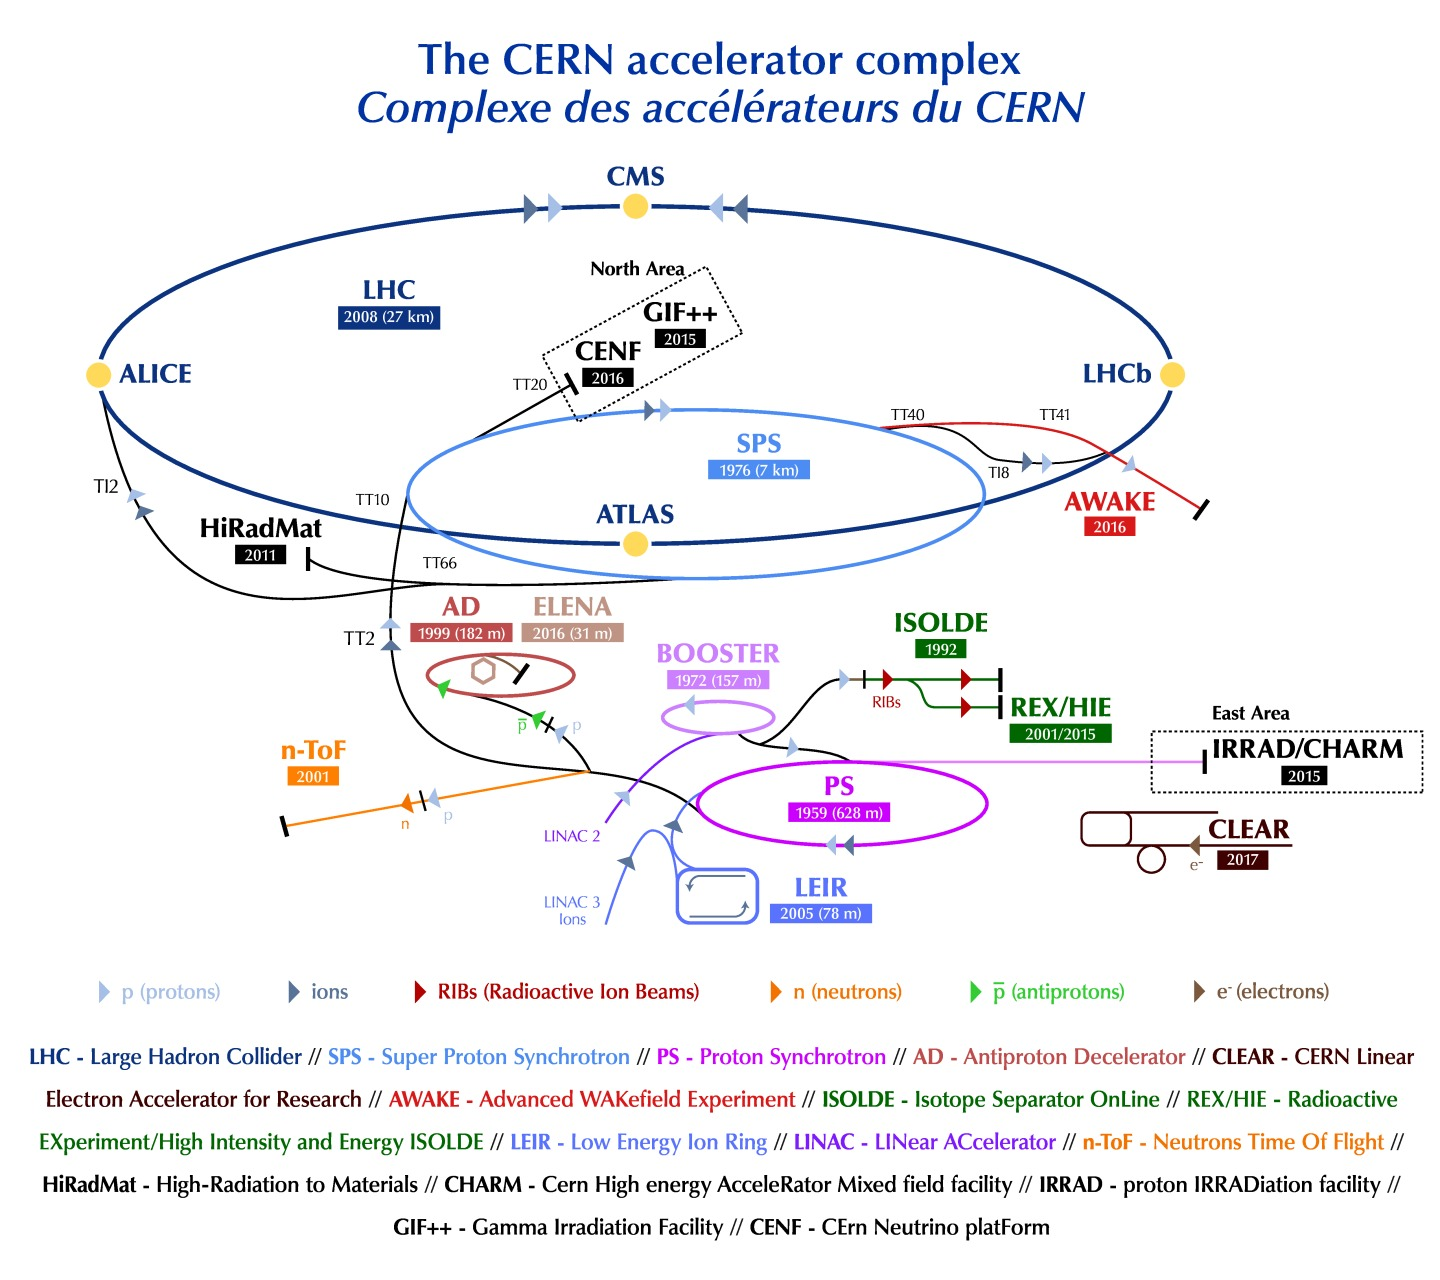
\includegraphics[width=0.8\textwidth]{Chapters/CH2/figures/CERN_complex}
	\caption{The overall CERN accelerator complex~\cite{CERN_complex}.}
	\label{fig:CERN_complex}
\end{figure}
\\The first step is the proton production from hydrogen gas and they are accelerated up to 50 MeV at the LINear ACcelerator 2 (LINAC 2). These protons are then injected into the 
Proton Synchrotron Booster (PSB) where their energy reach 1.8~GeV.  The acceleration chain continues into the Proton Synchrotron (PS) which pushes the beam
to 25~GeV. After that, the beam is injected into the Super Proton Synchrotron (SPS) where the protons are accelerated up to 450~GeV. Finally, the bunches of protons are injected in the LHC.
A typical bunch train corresponds to 2808 bunches for each beam with 25~ns separation and  bunch contains about $\mathrm{10^{11}}$ protons) colliding at a rate up to 40~MHz. 
\\The LHC is designed to accelerate each beam at an energy of 7~TeV thanks to a complex system of dipole and higher order magnets but the LHC performance has not always been 
those observed to the present day. \\
The first protons beams circulated in the LHC for the first time in September~\nth{10} of 2008. From 2010 to 2012, the protons
beams had an energy of 3.5~TeV. From 2012 to 2013, the energy reached was 4~TeV per beam. The first shutdown ended when the LHC started to accelerate
beams up to an energy of 6.5~TeV in April~\nth{5} of 2015.\\
Since protons are charged particles, a strong magnetic field, produced by 1232 superconducting electromagnets, curve the beams around the circular accelerator.
To maintain the superconductivity properties, these magnets requires a temperature of 1.9~K ($\mathrm{\approx}$271.3 \textdegree{}C). 
This temperature allows this dipole magnets to generate a magnetic field of 8~T. Besides this magnets, a total of 392 quadrupole magnets maintain the
beams focused and 16 radiofrequency cavities accelerate particles and keep them in controlled bunches with an constant energy.
Four main interaction points are used as collisions points corresponding to the location of the four detectors: ALICE, ATLAS, CMS and LHCb.\\
The beam in the LHC is not continuous but rather divided in a collection of protons (bunches) colliding at a rate up to 40 MHz. 
The LHC beam at full intensity nominally consists of 2808 bunches and each bunch contains $\mathrm{\approx 1.15 \times10^{11}}$ protons, spaced by 25~ns.\\
The number of multiple interactions per bunch crossing is called \textit{pile-up} and it is denoted by $\mathrm{\mu}$. 
Actually there are two different sources of pile-up:
\begin{itemize}
	\item in-time pile-up occurs when multiple collisions take place in a single bunch crossing
	\item out-of-time pile-up is due to finite read-out time resolution of the detectors, often larger than 25 ns. In this case, the residual energy from
	a previous bunch crossing could potentially be associated to the following bunch crossing.
\end{itemize}
\newpage
\noindent The distribution of $\mathrm{<\mu>}$ is shown in Figure~\ref{fig:pileup}, for the different data-taking periods. The average pile-up for 2015-2018 is $\mathrm{<\mu>=33.7}$.
\begin{figure}[h]
	\centering
	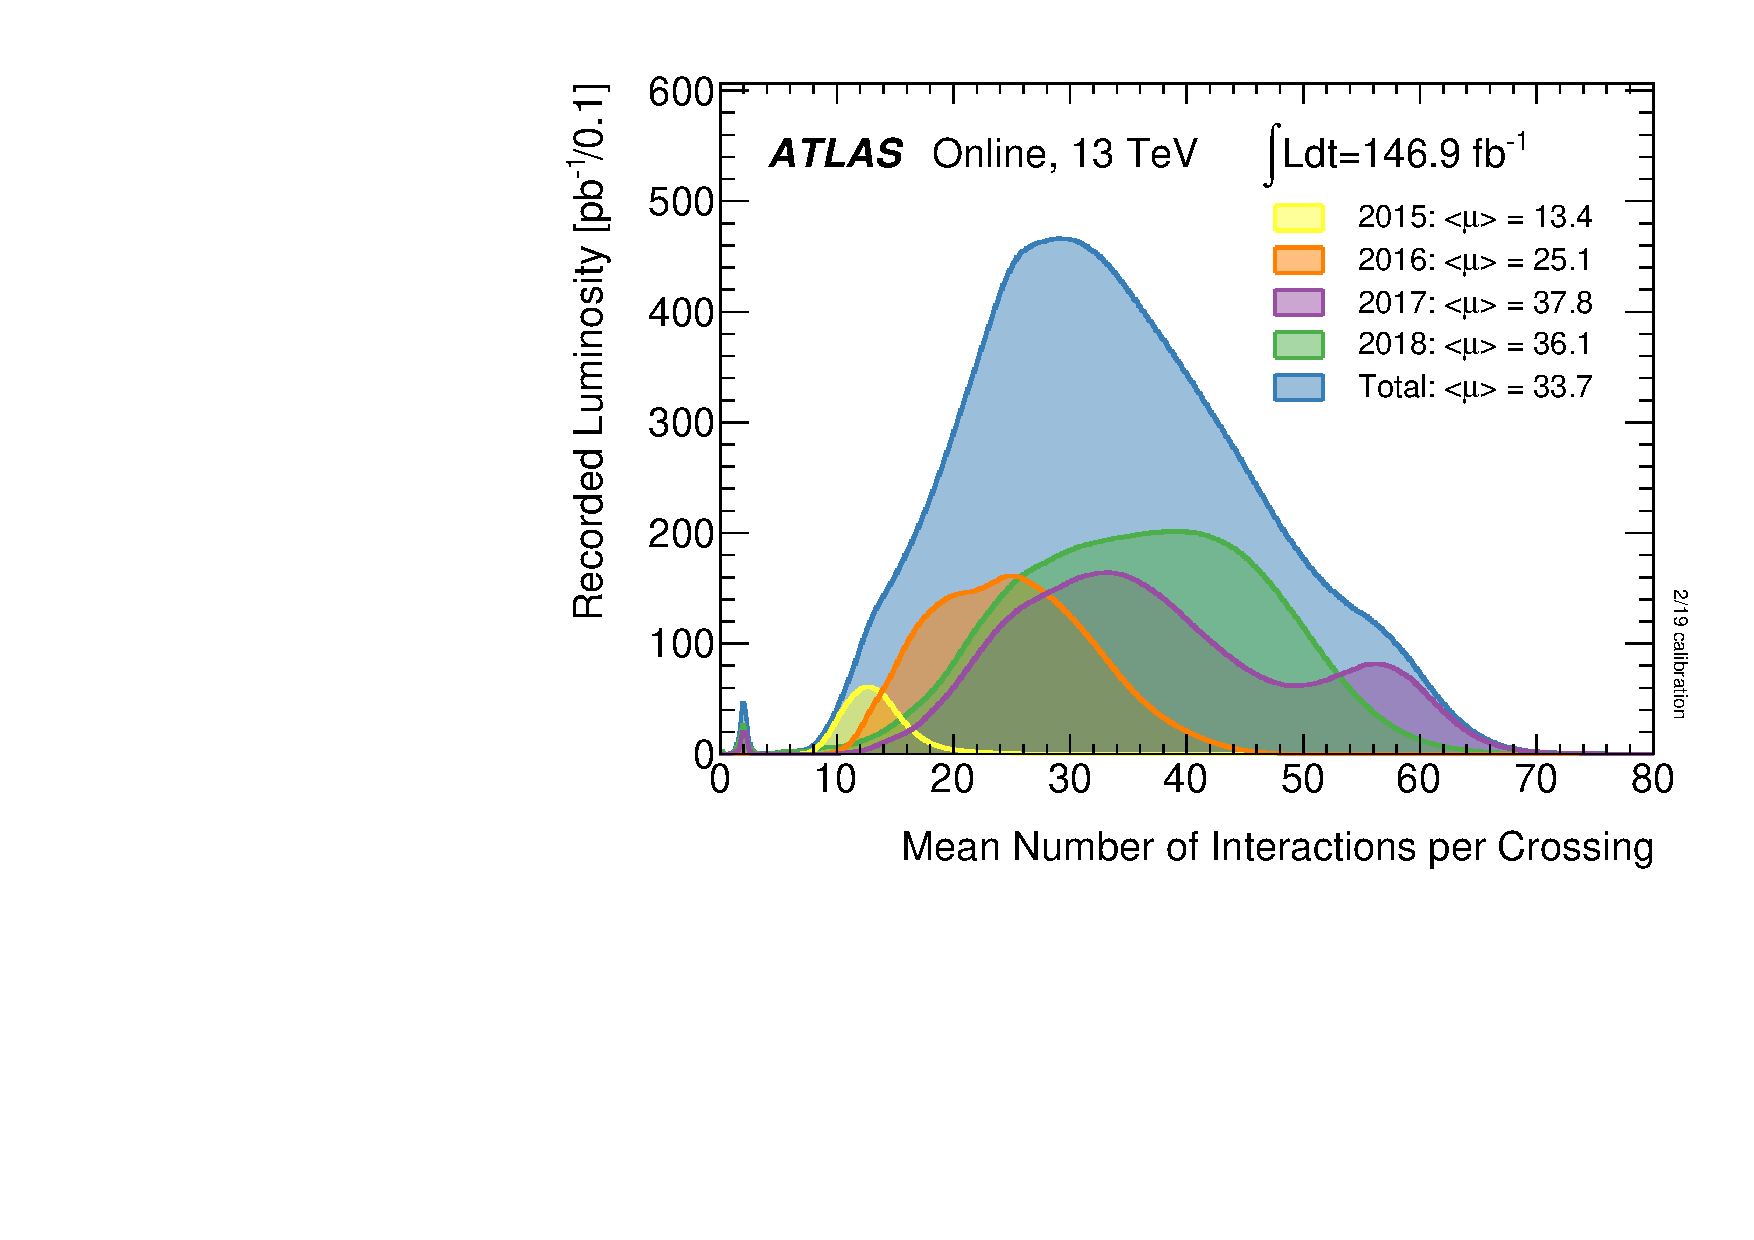
\includegraphics[width=9cm]{Chapters/CH2/figures/mu_2015_2018}
	\caption{Luminosity-weighted distribution of the mean number of interactions per crossing for the 2015-2018 pp collision data at $\mathrm{\sqrt{13}}$.  All data recorded by ATLAS during stable beams is shown, and the integrated luminosity and the mean mu value are given in the figure~\cite{lumi}.}
	\label{fig:pileup}
\end{figure}
\\The event rate of a given process with cross section $\sigma$ is given by $\frac{dN}{dt}=\mathcal{L} \sigma$, where $\mathcal{L}$ is 
a characteristic of the accelerator, known as \textit{instantaneous luminosity} and is given by:
\begin{equation}
\mathcal{L} =  \frac{N^{2}_{b}k_{b}f\gamma}{4\pi\sigma_{x}\sigma_{y}}F
\end{equation}
where $N^{2}_{b}$ is the number of particles per bunch, 
$k_{b}$ is the number of bunches, 
$\gamma$ represents the relativistic gamma factor, 
$f$ is the revolution frequency of the accelerator, 
$\sigma_{x}$ and $\sigma_{y}$ are the horizontal and vertical beam size, 
$F$ is a geometrical correction factor from the crossing-angle of the two beams at the interaction point (IP). 
\\Given a period of time T, one can define the \textit{integrated luminosity} as L= $\int^{T}_{0}{dt \mathcal{L}}$ 
which is typically expressed in $\mathrm{fb^{-1}}$ (1 $\mathrm{b = 10^{-28} m^{-2}}$).
\\Figure~\ref{fig:lum} shows the total integrated luminosity over the full LHC data taking period at $\mathrm{\sqrt{13}}$ TeV and Table~\ref{tab:lum} summarise the main design parameters of LHC.
\begin{figure}[h]
	\centering
	\subfigure[]{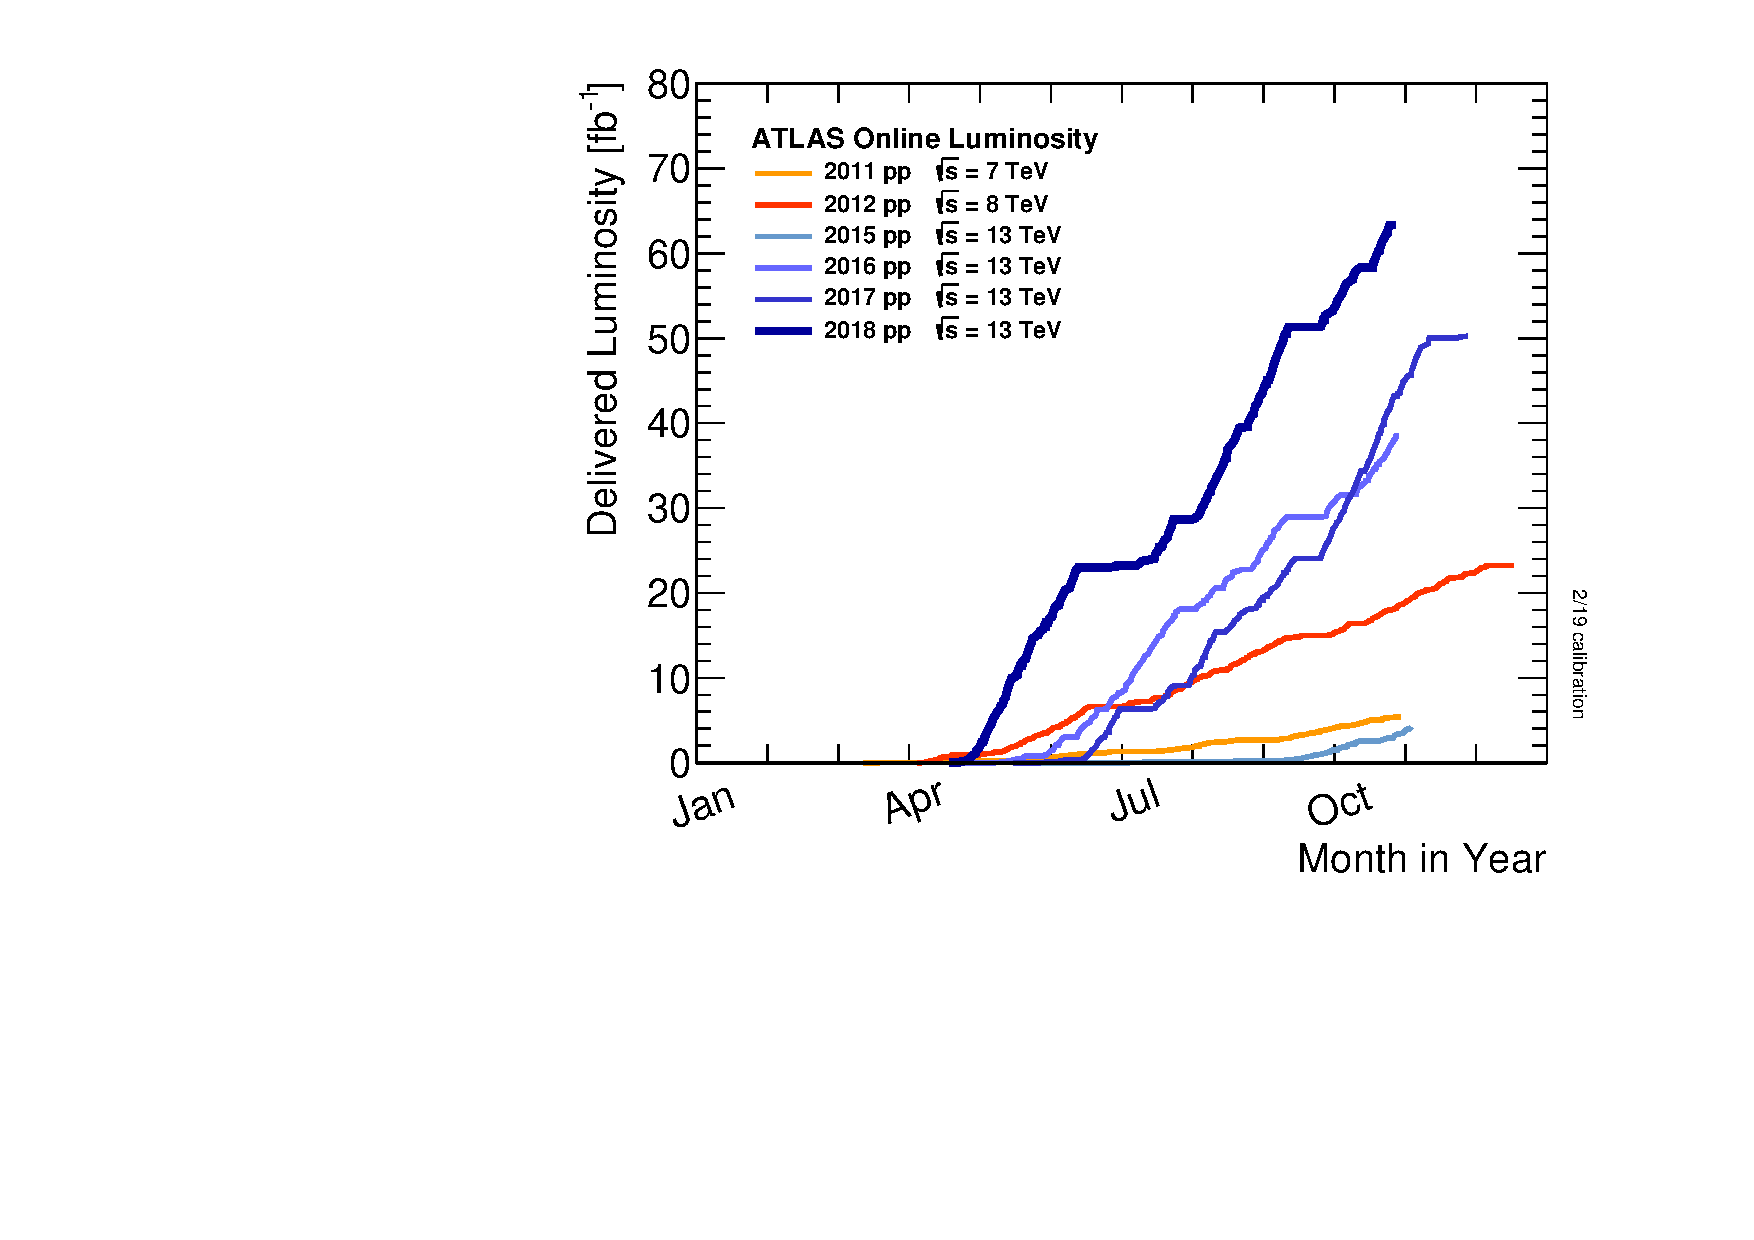
\includegraphics[width=55mm]{Chapters/CH2/figures/intlumivsyear}}\quad
	\subfigure[]{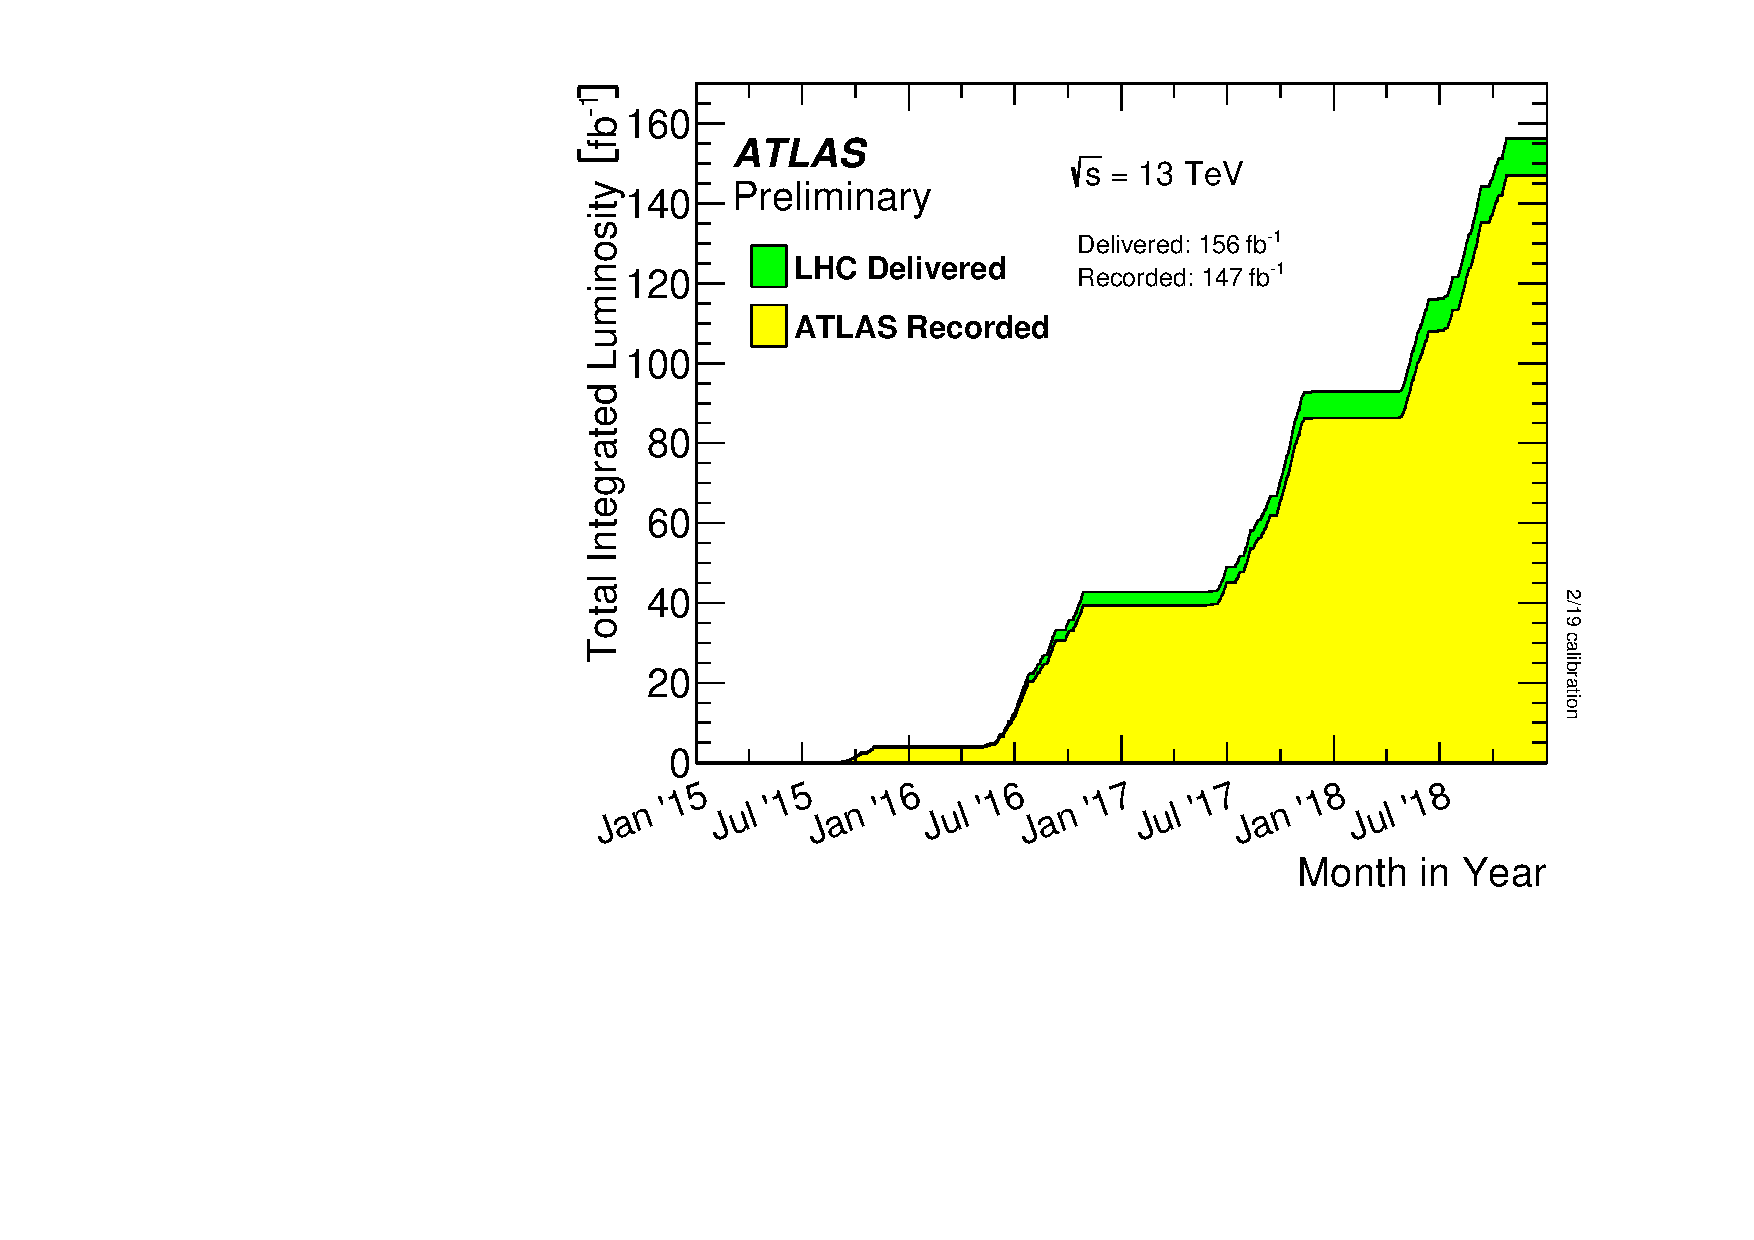
\includegraphics[width=55mm]{Chapters/CH2/figures/intlumivstimeRun2}}\quad
	\caption{Cumulative luminosity versus ($a$) day delivered to ATLAS during stable beams; ($b$) time delivered to ATLAS (green) and recorded by ATLAS (yellow) during stable beams for pp collisions at $\mathrm{\sqrt{13}}$~\cite{lumi}.}
	\label{fig:lum}
\end{figure}
\begin{table}[h]
	\begin{adjustbox}{max width=1.\textwidth,center}
		\begin{tabular}{lcccc}
			\hline 
			\textbf{Parameter}              											&  \textbf{2015} & \textbf{2016} 			& \textbf{2017} & \textbf{2018} \\ 
			\hline 
				Bunch intensity [$\mathrm{\times10^{11}p}$] 		  &  1.2 				  & 1.1 						  & 1.25 				& 1.15 				\\
				Number of bunches   												 &  2200 			   & 2200						 & 1900				  & 2500			\\
				Emittance [$\mathrm{\mu m}$] 							 	  & 3.5					  & 2.5 						  &2.0 					 & 2.2				 \\
				Crossing angle [$\mathrm{\mu rad}$] 					   & 290 				  & 280 						 & 300 				   & 300		      \\
				Peak luminosity [$\mathrm{10^{34} cm^{2}s^{-1}}$] 	& 0.5 					& 1.5 							& 1.5				   &  2.0				\\
			\hline  
		\end{tabular} 
	\end{adjustbox}
	\caption{Main beam parameters of proton-proton collisions of LHC in Run2.}
	\label{tab:lum}
\end{table} 
\FloatBarrier
\section{The ATLAS detector}
ATLAS (A Toroidal LHC ApparatuS)~\cite{ATLAS} is a multi-purpose apparatus whose primary goal is to identify and measure the properties of particles produced in p-p collision.\\
The overall ATLAS detector layout is shown in Figure~\ref{fig:ATLAS}.\\
The ATLAS detector consist of a concentric cylinder shape (4$\pi$ coverage), therefore nominally forward-backward symmetric with respect to the interaction point (IP) where the proton beams collide in it.
It can be divided into five main parts:
\begin{itemize}
	\item Magnet System (section~\ref{sec:MagSys});
	\item The Inner Detector  (section~\ref{sec:ID});
	\item The Calorimetric System  (section~\ref{sec:CAL});
	\item Muon Spectrometer  (section~\ref{sec:MuonSpec}).
	\item Trigger and data acquisition System  (section~\ref{sec:TrigSys}).
\end{itemize}
\begin{figure}[h]
	\centering
	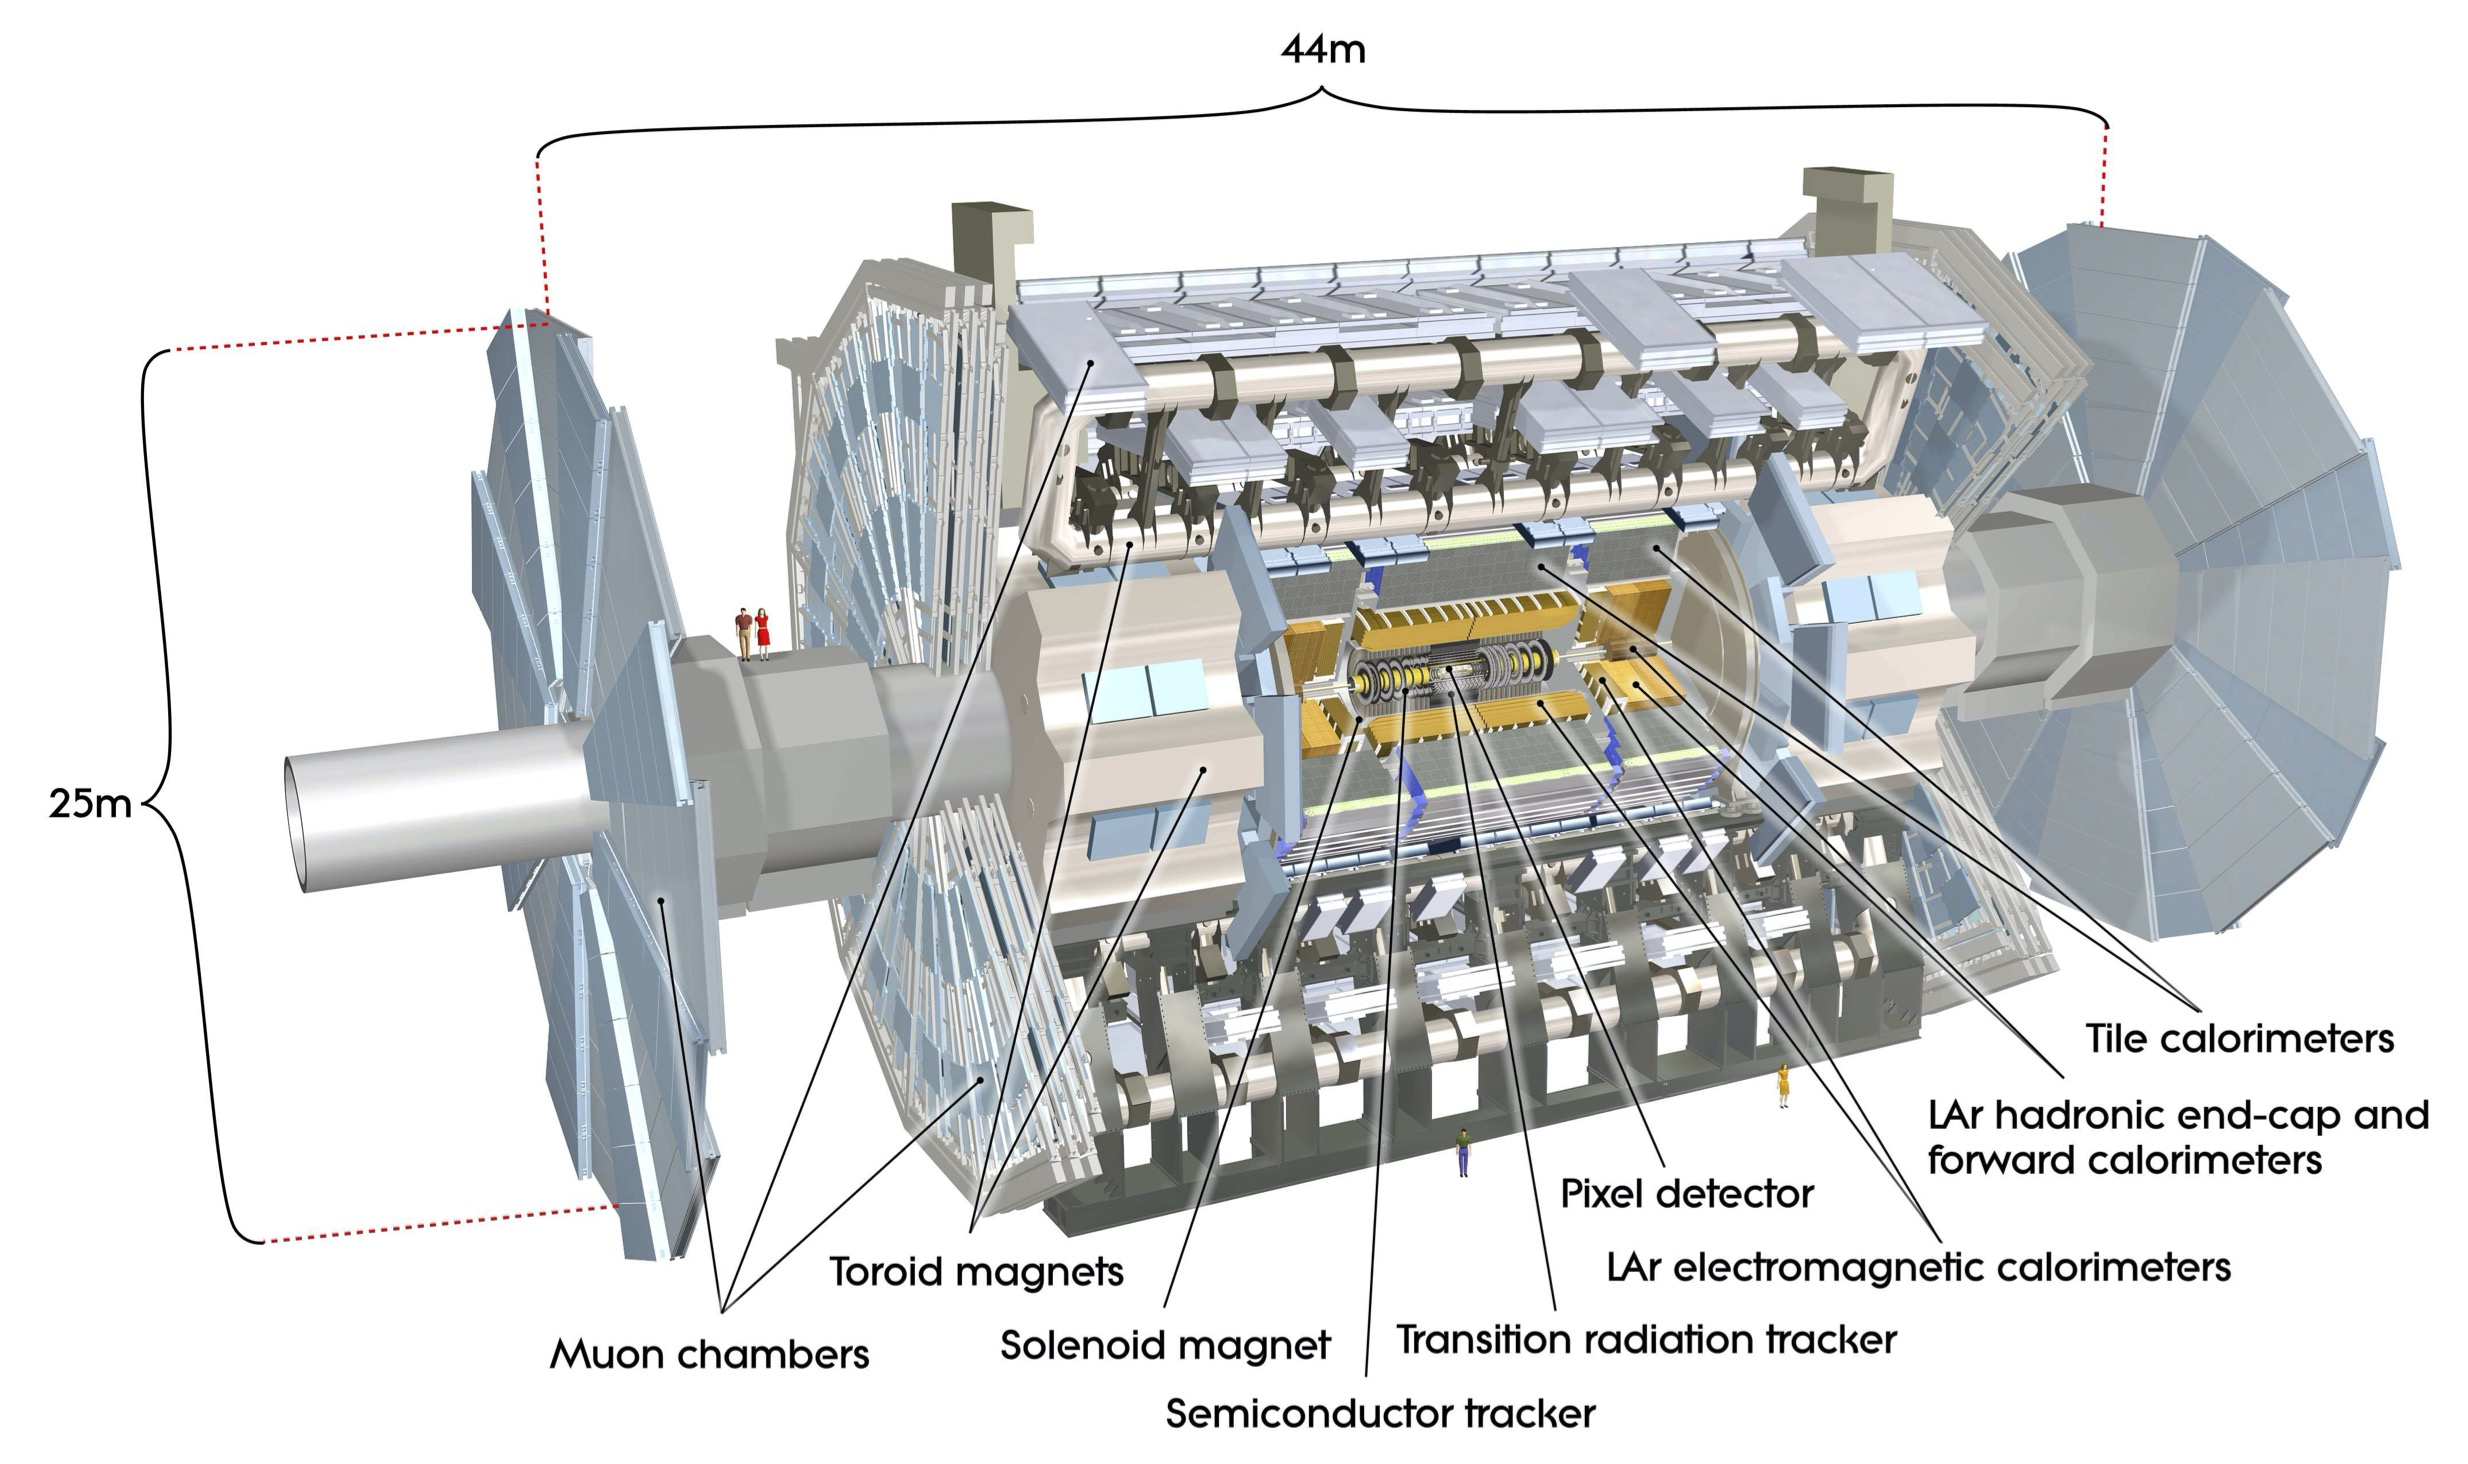
\includegraphics[width=10cm]{Chapters/CH2/figures/ATLAS}
	\caption{Cut-away view of the ATLAS detector. The dimensions of the detector are 25 m in height and 44 m in length. The overall weight of the detector is approximately 7000 tonnes~\cite{ATLAS}.}
	\label{fig:ATLAS}
\end{figure}
\FloatBarrier
\subsubsection*{Coordinate system}
The ATLAS coordinate system is a right-handed Cartesian coordinate system with the origin defined at the IP, in the center of the detector.\\
The $z$-axis corresponds to the beam pipe while the $x$ and $y$ directions define the transverse plane.\\
A cylindrical coordinate system is often used due to the geometry of the detector, where $\phi$ is the azimuthal angle and $\theta$ is the polar angle. 
$\phi$ is orthogonal to the beam direction, therefore it is invariant under a Lorentz boost($z$-axis), while $\theta$ is not an invariant, so the \textit{pseudorapidity} is defined as:
\begin{equation}
\eta=-\ln{(\tan{\bigg(\frac{\theta}{2}\bigg)})}
\end{equation}
Pseudorapidity is an approximation of the \textit{rapidity}\footnotemark for relativist particles ($m\ll p$).
\footnotetext{Rapidity is defined as $y=\frac{1}{2}\ln{\frac{E+p_z}{E-p_z}}$}
\\The distance between two objects is indicated using $\mathrm{\Delta R}$, defined as:
\begin{equation}
\Delta R =\sqrt{\Delta \eta^{2}+\Delta \phi^{2}}
\end{equation}
The transverse momentum is the projection of the momentum orthogonal to the beam direction is defined as:
\begin{equation}
p_{T}=\sqrt{p^{2}_{x}+p^{2}_{y}}
\end{equation}

\subsection{Magnet System}
\label{sec:MagSys}
The magnet configuration comprises a thin superconducting solenoid surrounding the inner-detector cavity, and three large superconducting toroids (one barrel and two end-caps) arranged with an eight-fold azimuthal symmetry around the calorimeters. This fundamental choice has driven the design of the rest of the detector.\\
The inner detector is immersed in a 2 T solenoidal field provided by the central solenoid with inner radius of 1.23 m and a total length of 5.8 m.\\
It is designed to minimize the amount of material in front of the calorimeter to have a small impact on the energy measurement. This is achieved by hosting the solenoid and
the cryostat in the same vacuum vessel of the electromagnetic calorimeter.\\
The overall dimensions of the magnet system is 26 m long and 20 m diameter and provide and average magnetic field intensity of 0.5 T in the barrel and 1 T in the end-caps regions~\cite{MagSys}.

\subsection{Inner Detector}
\label{sec:ID}
The Inner Detector (ID)~\cite{ATLAS} is the detector system closest to the beam.\\
It is composed of three detectors: the semiconductor pixel detector (PIXEL), the microstrip detector SCT (Semi-Conductor Tracker), and the most external, the transition radiation detector TRT (Transition Radiation 
Tracker).\\
Its overall layout is depicted in Figure~\ref{fig:ID}.
\begin{figure}[h]
	\centering
	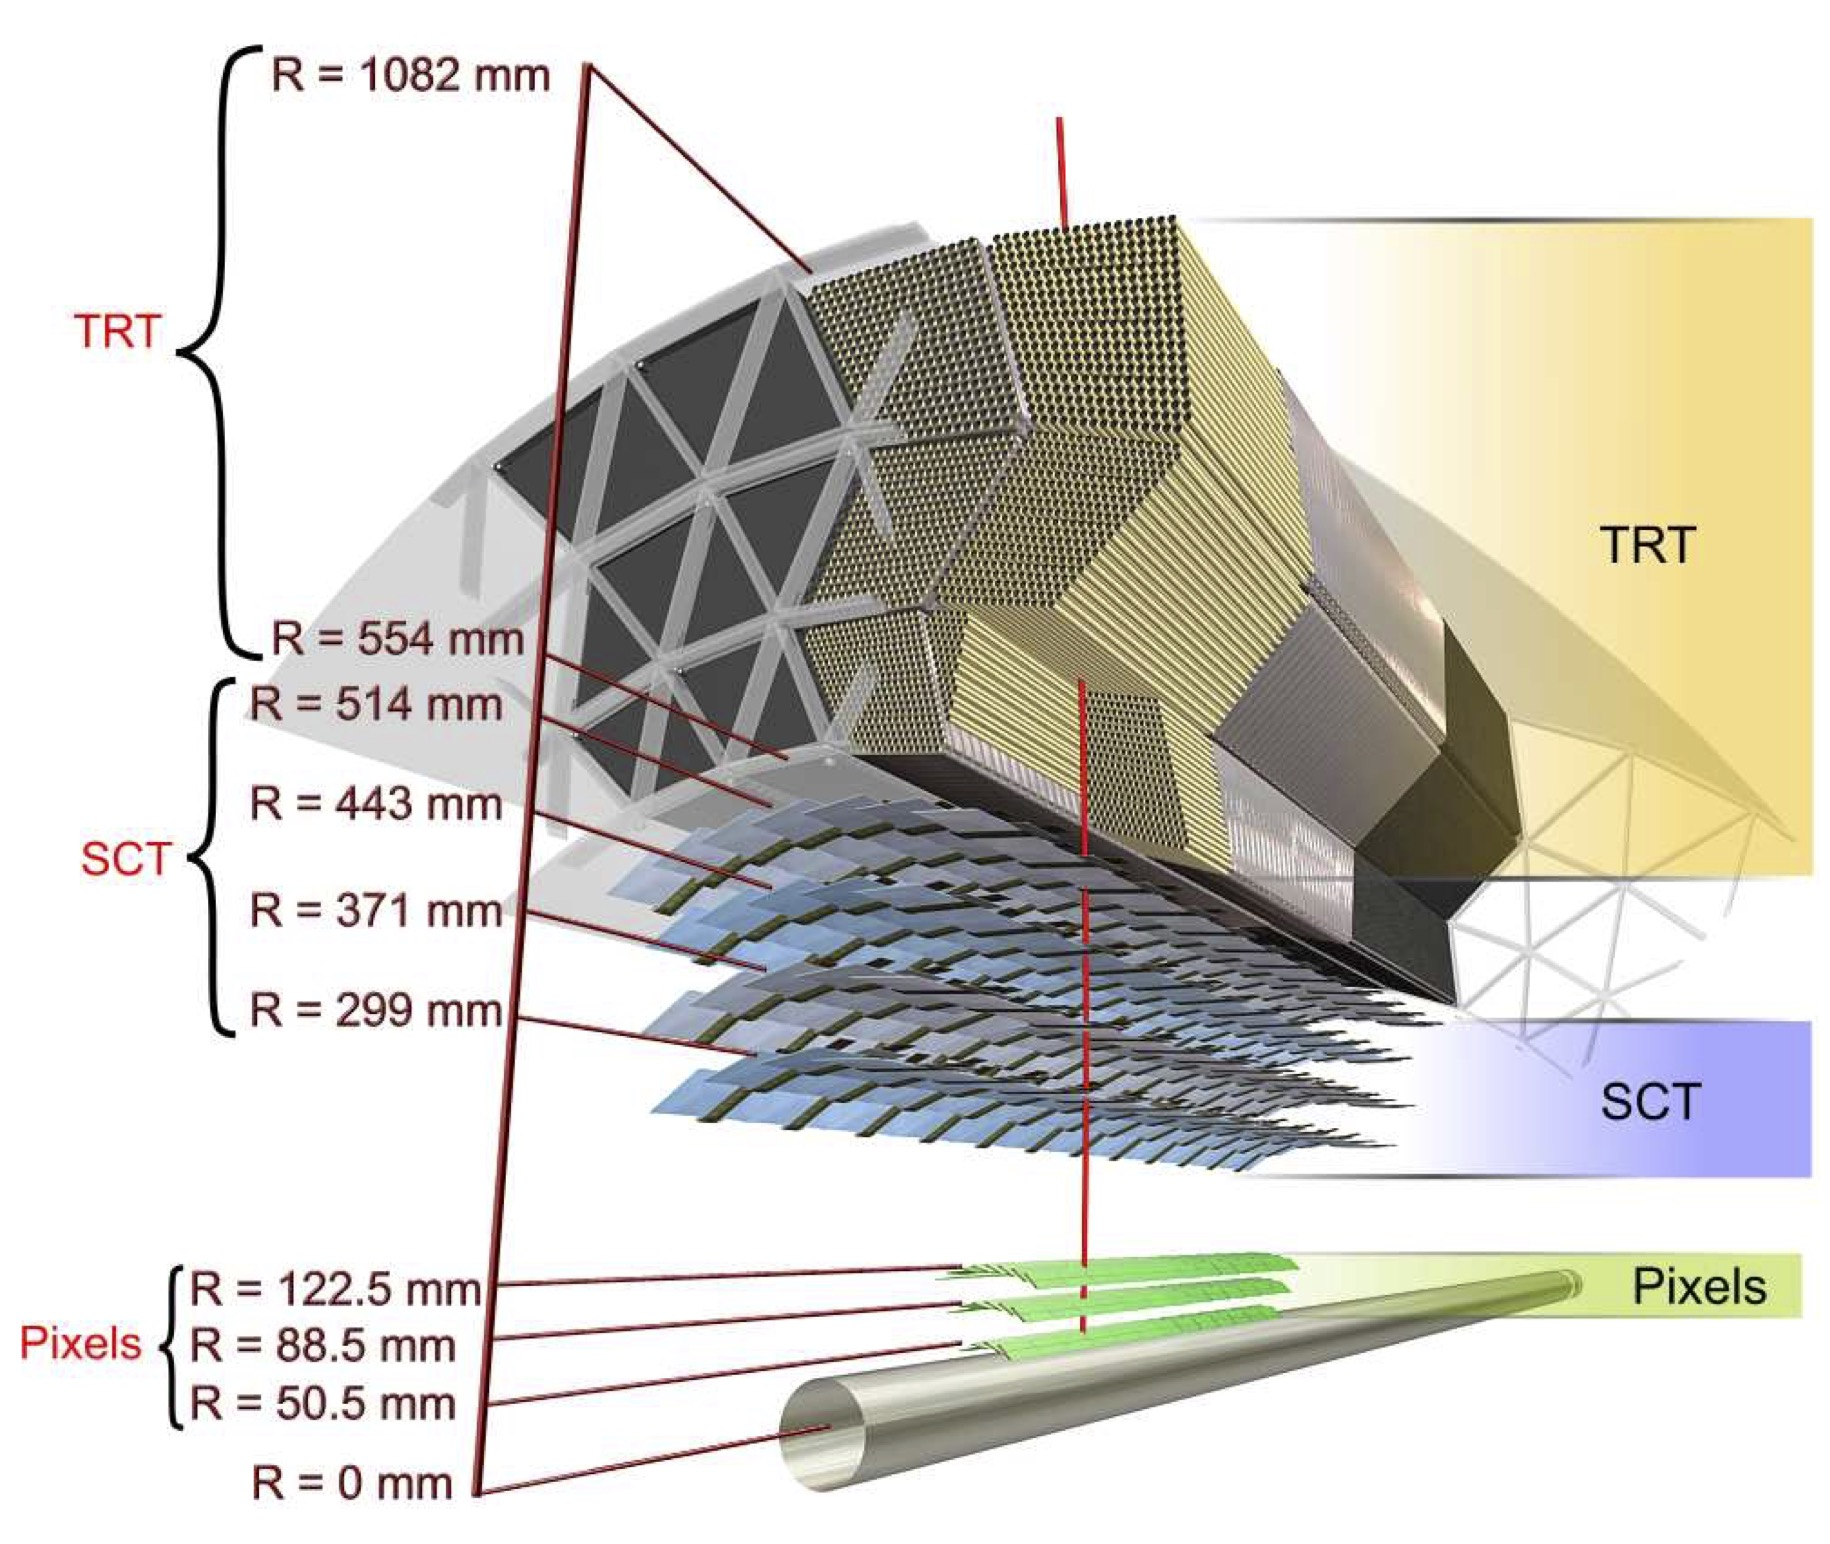
\includegraphics[width=9cm]{Chapters/CH2/figures/ID}
	\caption{Schematic view of the barrel of the ATLAS inner tracking system~\cite{ATLAS}.}
	\label{fig:ID}
\end{figure}
\\The ID is contained in a cylinder 7 m long and 1.15 m in radius, placed in a 2 T solenoid magnetic field and it is designed to trace charged particles with a minimum moment of 0.1 GeV/c to allow the measurement of the moment through the curvature radius and the reconstruction of the main interaction and decay vertices (both primary and secondary).\\
The innermost part of the ID, which has a radius of about 15 cm, consists of silicon pixels to maximize the precision in the reconstruction of the tracks and the resistance to radiation.
The pixel detector records on average three points for each track, which allows a reconstruction of the secondary decay vertices. This detector has a total of approximately 80 million sensitive elements.
\vspace{\baselineskip}
\\The intermediate part, which covers a radius ranging from 30 to 60 cm, uses a microstrip detector (Semi-Conductor Tracker), to provide good spatial resolution.
The detection technique of the SCT relies on the same principle as for the pixel detector, however long strips are used compared to the rectangular pixels due to 
the smaller particle density in the outer layers.
It is built around the Pixel detector and is designed to provide eight precision measurements per track, contributing to the measurements of momentum, impact parameter and 
vertex position. The total number of sensitive items is around 6 million.
\vspace{\baselineskip}
\\The outermost layer ranges from 60 to 95 cm in radius; it is a gas detector (Transition Radiation Tracker) consisting of a set of small diameter tubes, containing $\mathrm{Xe}$ ($\mathrm{70\%}$), 
$\mathrm{CO_2}$ ($\mathrm{27\%}$),  $\mathrm{O_2}$ ($\mathrm{3\%}$); it provides a good resolution of the curvature of the track and contributes strongly to its reconstruction.\\\
The tracker contributes to the identification of the electrons, being sensitive to the emission of transition radiation that the particles emit when passing between different materials. 

\subsection{Calorimetric System}
\label{sec:CAL}
Calorimeters must provide good containment for electromagnetic and hadronic showers, they must limit punch-through into the muon system, and finally they must detect the particles that do not lose energy by ionization and are therefore not seen by the internal detector.\\
It is important that calorimeters cover most possible portion of solid angle; in fact, if a particle pass through a region without instrumentation, it is not detected and its energy contributes to the \textit{Missing 
Transverse Energy} (MET), the precision of which is essential for identifying and studying weakly interacting particles such as neutrinos and possibly, new BSM particles. \\
In ATLAS there are two calorimeters: the Electromagnetic Calorimeter (ECAL)  and the Hadron Calorimeter (HCAL), as depicted in Figure~\ref{fig:cal} and they cover the range $\mathrm{|\eta<4.9|}$.  
\begin{figure}[h]
	\centering
	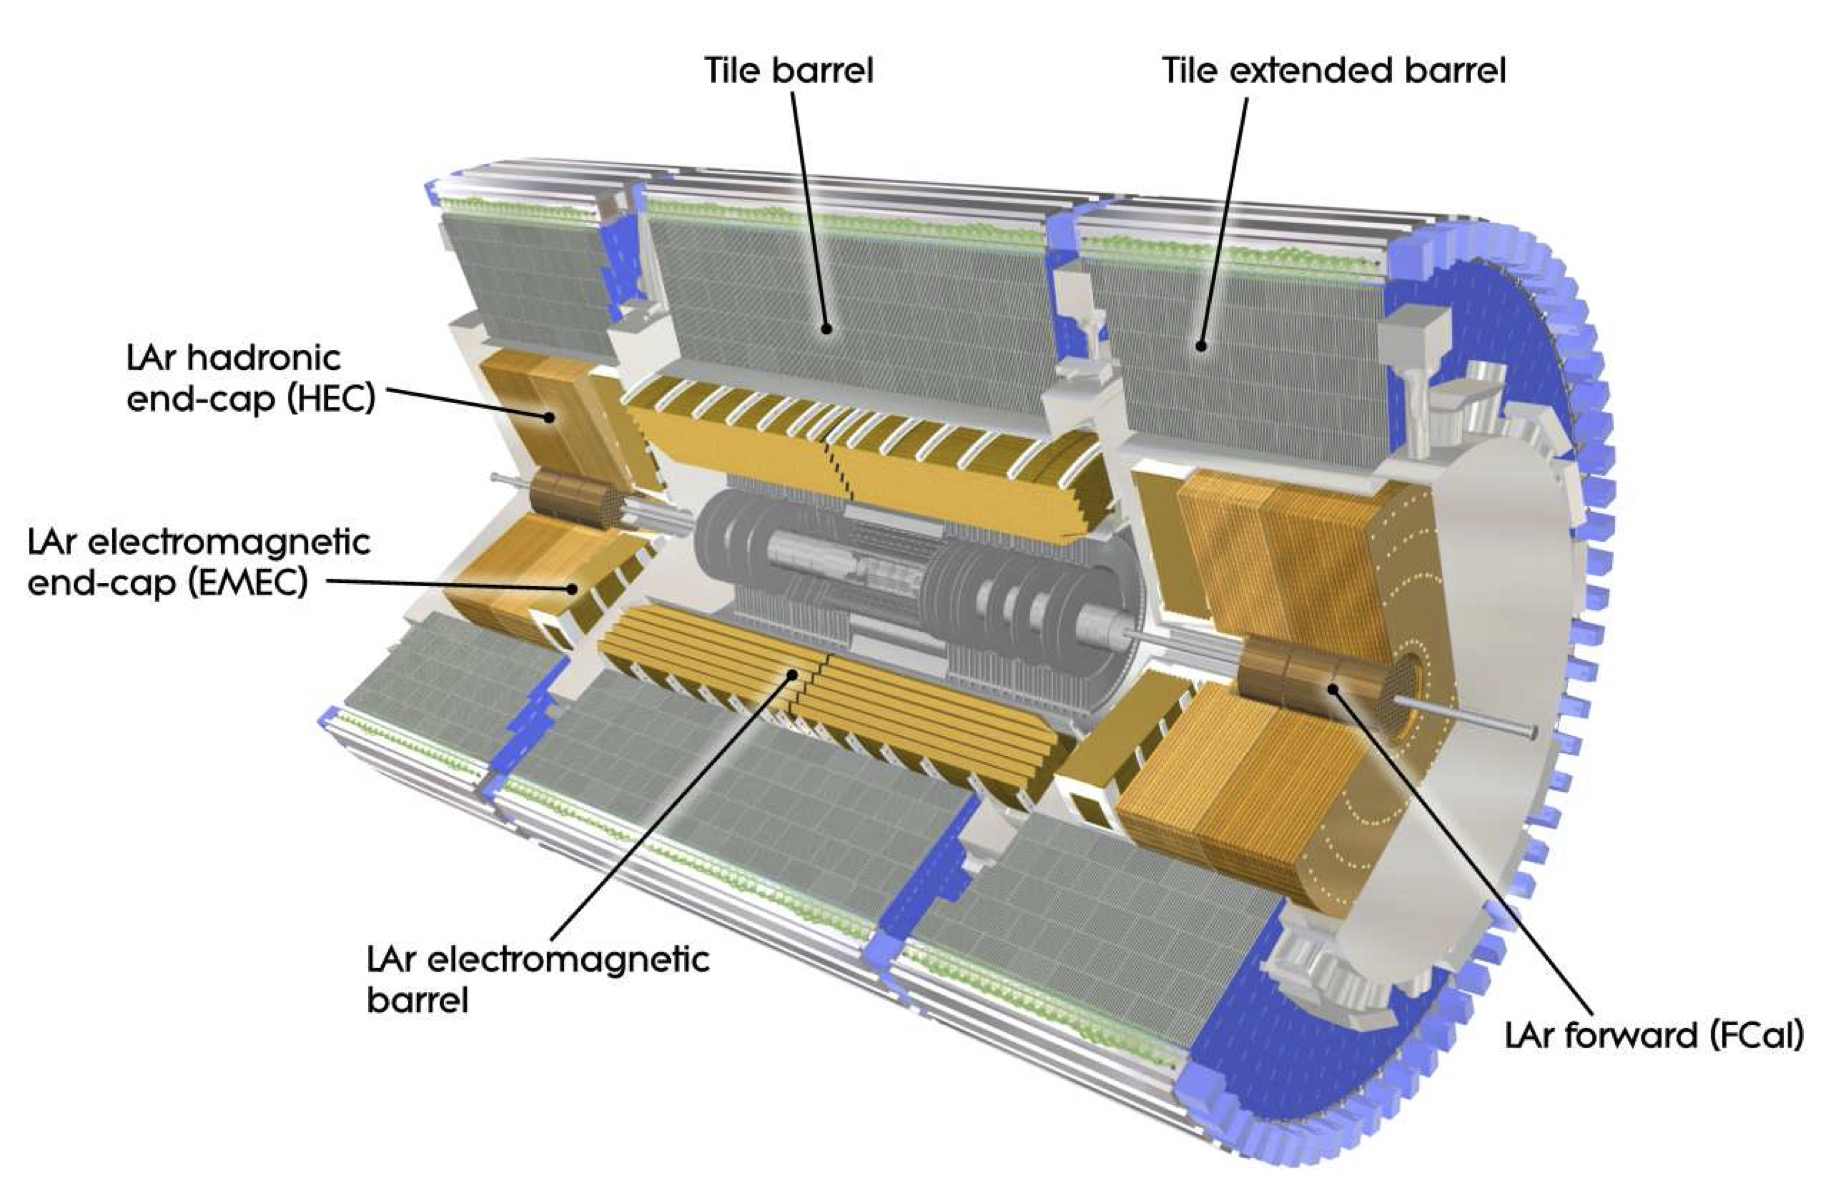
\includegraphics[width=10cm]{Chapters/CH2/figures/cal}
	\caption{Cut-away view of the ATLAS calorimeter system~\cite{ATLAS}.}
	\label{fig:cal}
\end{figure}
\newpage 
\noindent The ECAL is divided into a barrel part ($\mathrm{|\eta|<1.475}$) and two end-cap components ($\mathrm{1.375<|\eta|<3.2}$), each housed in their own cryostat.\\
It is a lead-LAr detector with accordion-shaped kapton electrodes and lead absorber plates over its full coverage. The accordion geometry provides complete $\phi$ symmetry without azimuthal cracks.
The lead thickness in the absorber plates has been optimised as a function of $\eta$ in terms of ECAL performance in energy resolution. 
\\A schematic representation of the ECAL in the barrel and its main construction parameters are shown in Figure~\ref{fig:ECAL}. 
\begin{figure}[h]
	\centering
	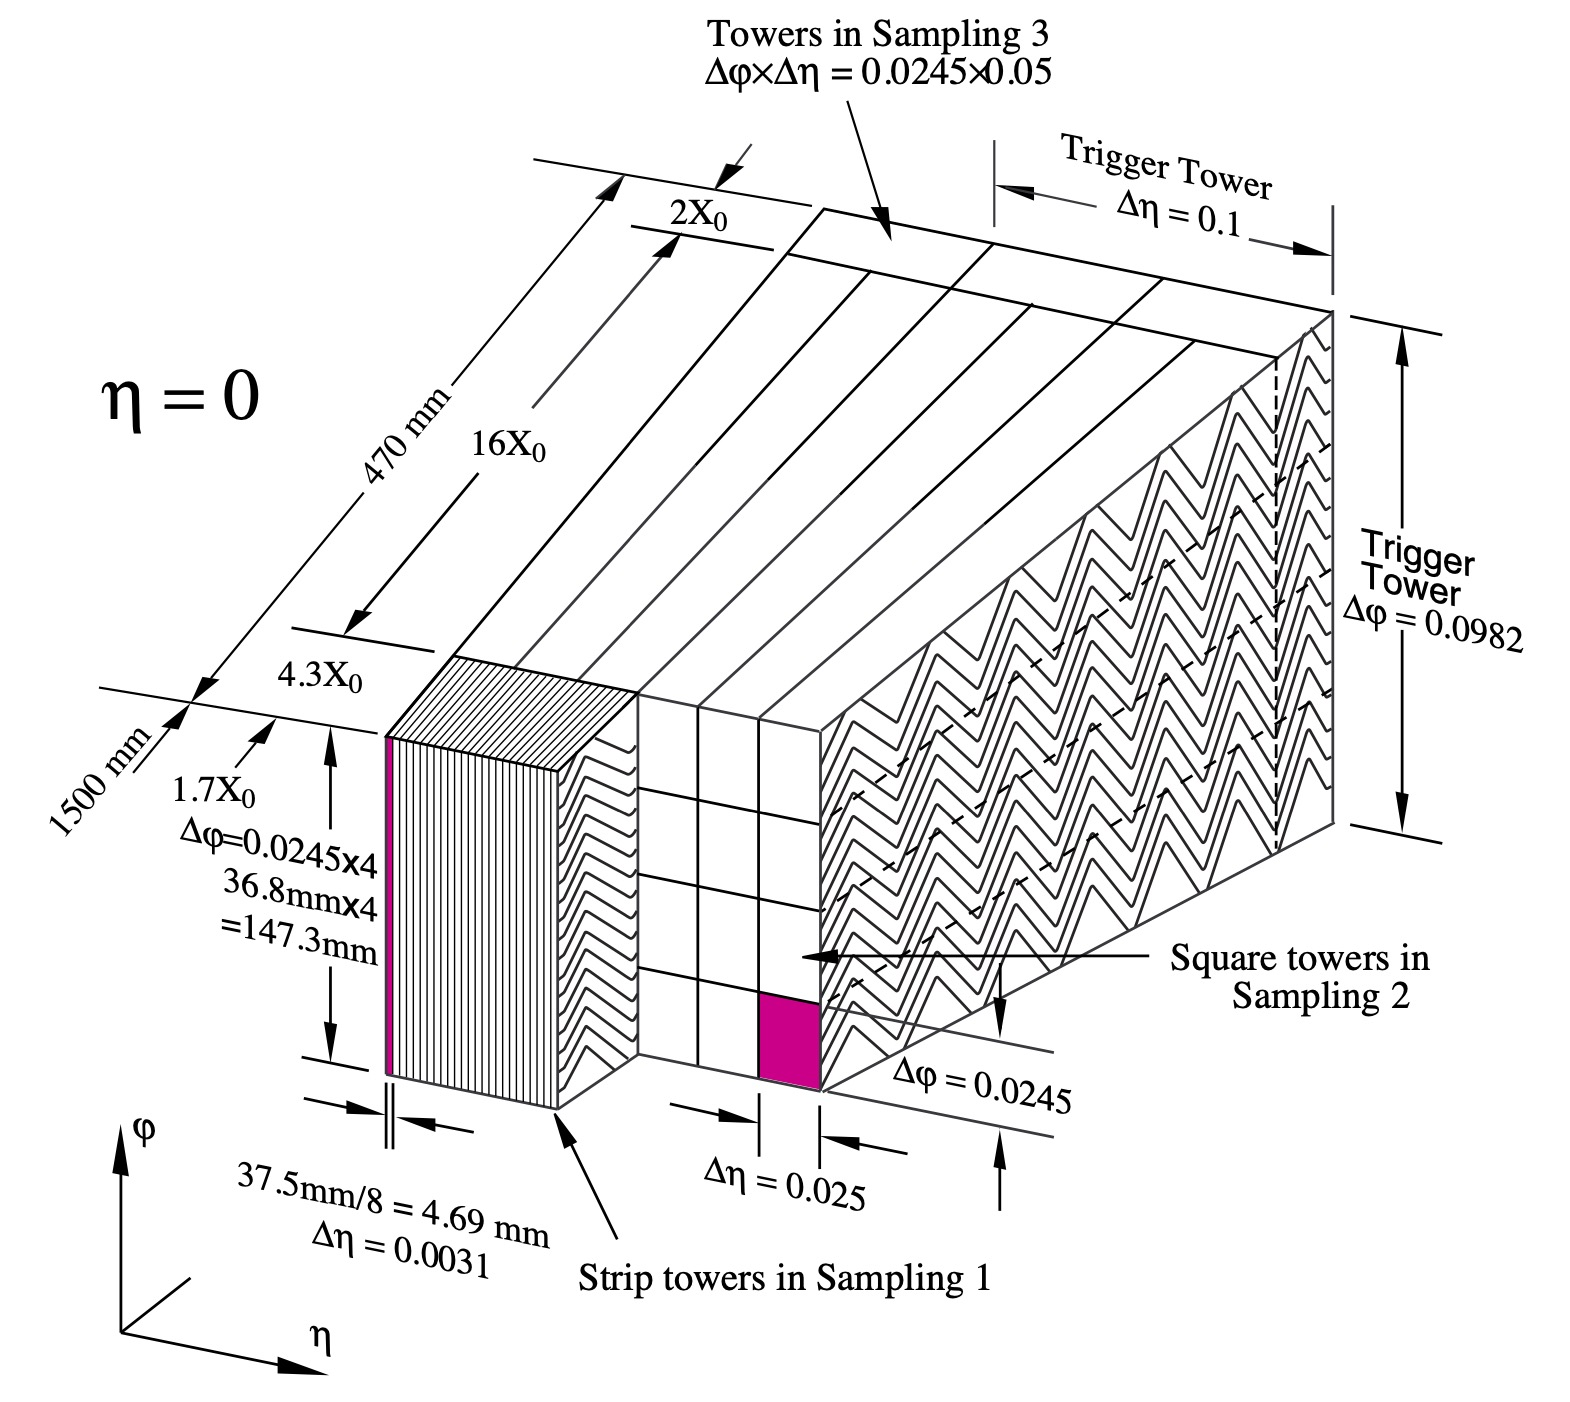
\includegraphics[width=7cm]{Chapters/CH2/figures/ECAL}
	\caption{Sketch of the accordion structure of the ECAL~\cite{cal}.}
	\label{fig:ECAL}
\end{figure}
\vspace{\baselineskip}
\\The outer calorimeter is the HCAL, which is divided in Tile Calorimeter (TileCal), the Hadronic End-cap Calorimeter (HEC) and the Forward Calorimeter (FCal). \\
LAr technology is also used for the hadronic calorimeters, matching the outer $|\eta|$ limits of end-cap electromagnetic calorimeters. 
The tile calorimeter barrel covers the region $\mathrm{|\eta|<1.0}$, and its two extended barrels the range $\mathrm{0.8<|\eta|<1.7}$ and it is a sampling calorimeter 
using steel as the absorber and scintillating tiles as the active material.\\
The HEC consists of two independent wheels per end-cap, located directly behind the end-cap electromagnetic calorimeter and the technology is similar to that of the 
electromagnetic one in the end-cap region, the active medium is LAr, but the absorption medium is made of copper rather than lead.
The FCal ($\mathrm{3.1<|\eta|<4.9}$) is integrated into the end-cap cryostats, as this provides clear benefits in terms of uniformity of the calorimetric coverage as well as reduced radiation background levels in 
the muon spectrometer. The FCal consists of three modules in each end-cap: the first, made of copper, is optimised for electromagnetic measurements, while the other two, made of tungsten, measure 
predominantly the energy of hadronic interactions.\\
An important quantity to mention is the energy resolution which is parameterized as:
\begin{equation}
\frac{\sigma_{E}}{E}=\frac{S}{\sqrt{E}} \oplus \frac{N}{E} \oplus C
\end{equation}
The first term represent the stochastic contribution related to the shower evolution, the second term
is related to the read-out electronics and the effect of the pile-up. The last term is a costant, due to systematic effects (e.g. mis-calibrations, dead detector material). 
The dominant source of uncertainty is linked, at low energy, with the high pile-up whereas, at high energy, C becomes the leading uncertainty. 

\FloatBarrier
\subsection{Muon Spectrometer}
\label{sec:MuonSpec}
The calorimeter is surrounded by the Muon Spectrometer (MS) depicted in Figure~\ref{fig:MS}, which is placed at the outermost part of the ATLAS detector.\\
The outer layers are reached by a few types of particles, mainly muons and neutrinos.\\
Those muons ionise  with the materials passed through since they are charged particles but the energy, that muons lose by the electromagnetic interaction
with other nuclei, is not such as to brake them until absorption. 
However the MS  identify them and measure their momentum.
\begin{figure}[h]
	\centering
	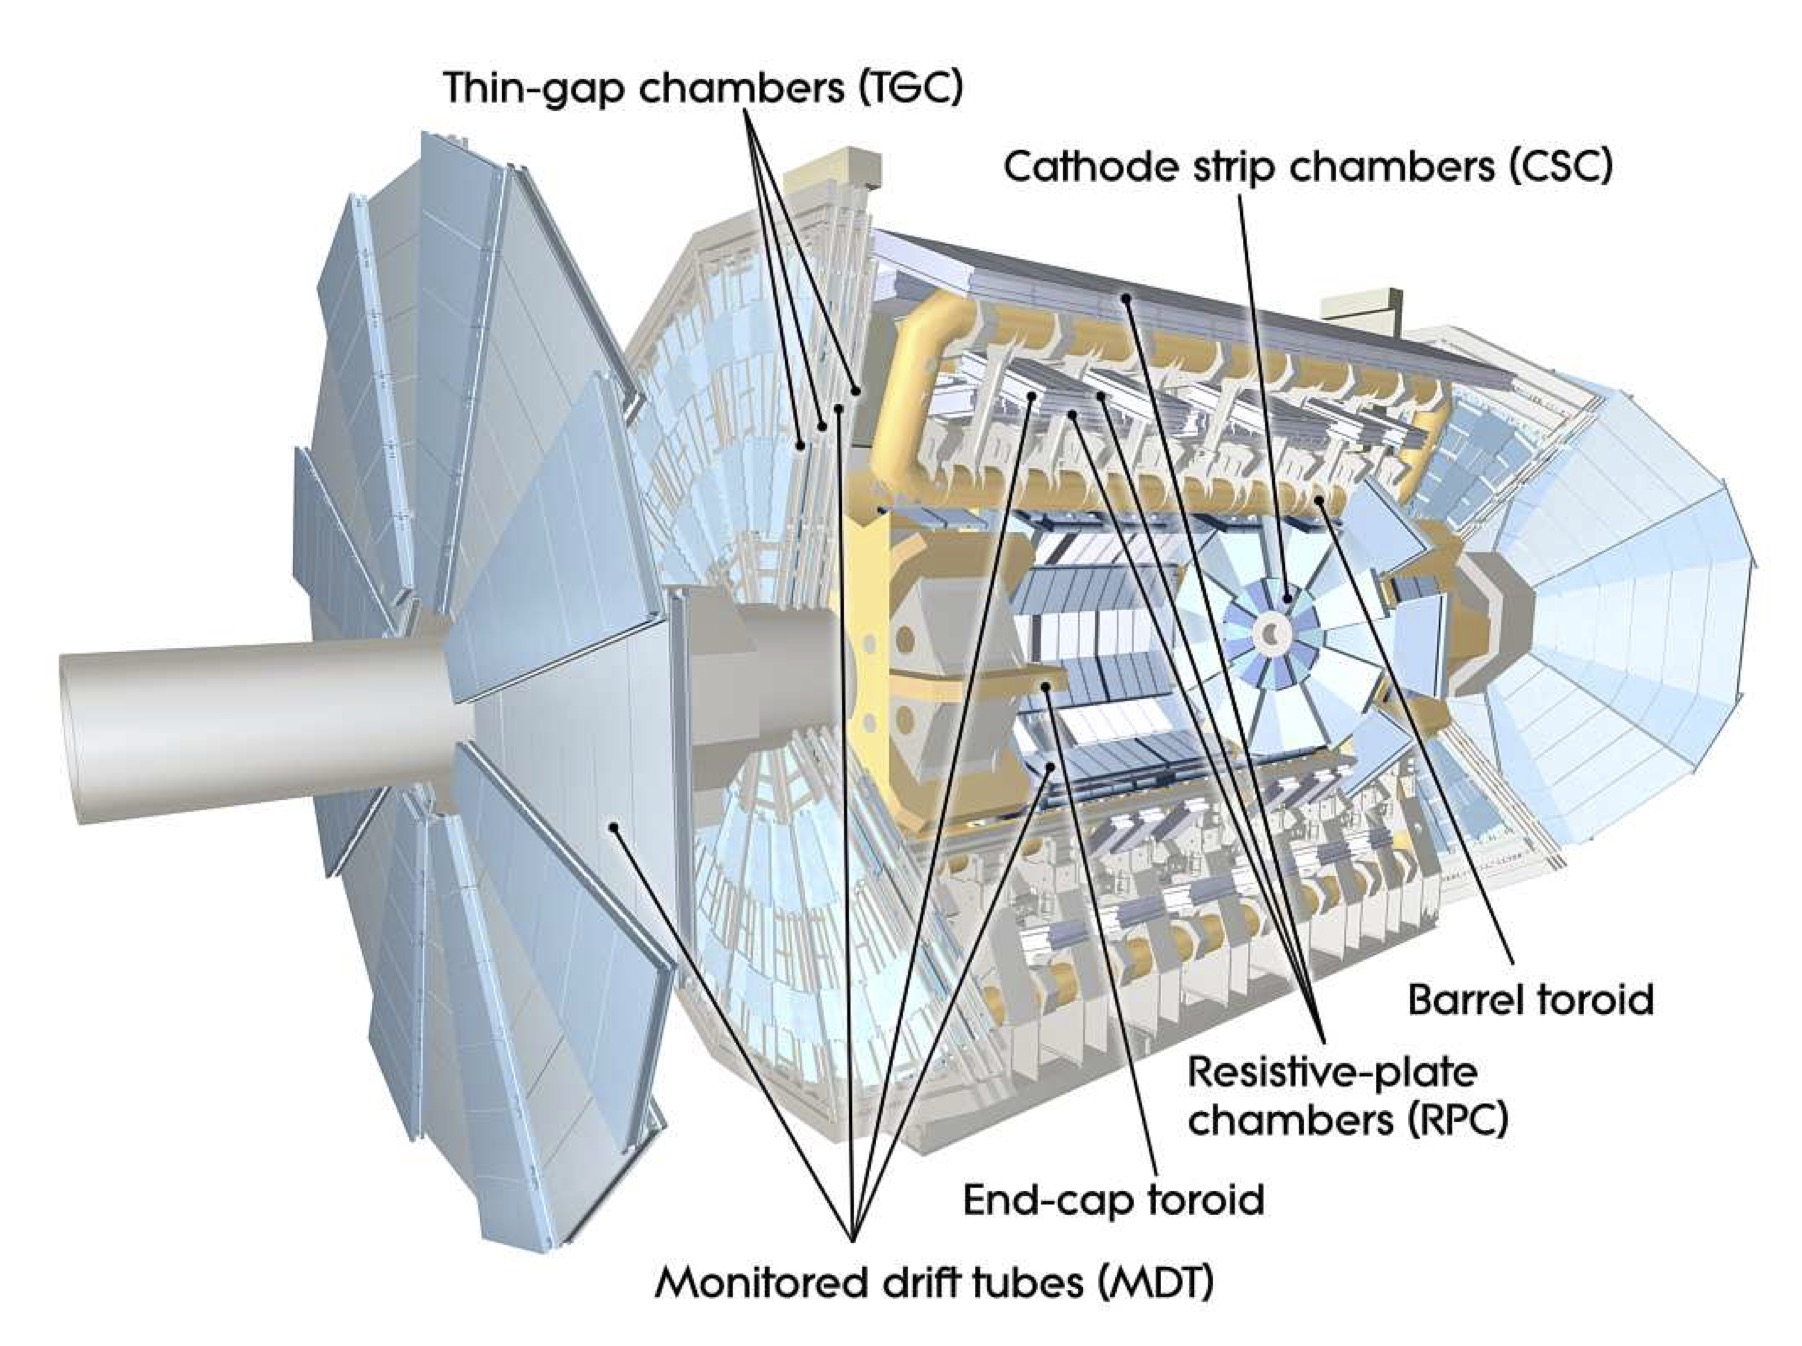
\includegraphics[width=10cm]{Chapters/CH2/figures/MS}
	\caption{Cut-away view of the ATLAS muon system~\cite{ATLAS}.}
	\label{fig:MS}
\end{figure}
\\A series of magnets arranged externally to the calorimeter creates a toroidal-shaped magnetic field
that modify the charged particles direction allowing the measurement of the momentum.
For muons with $\mathrm{p_T}$ > 30 GeV the measurement is much more precise than the measurement obtained by the internal detector. 
For lower $\mathrm{p_T}$, on the other hand, the measurement is less accurate, due to the 
energy loss in the previous layers of the detector and taken in to account to handle \textit{soft muons}, presented in Chapter~\ref{chapter:smt}.\\
For both the central part and the end-caps,  there are two types of detectors:
\begin{itemize}
	\item a trigger system based on cameras with fast response, such as the \textit{Resistive Plate Chamber} (RPC) and the \textit{Thin Gap Chamber} (TGC), 
	\item precision tracking chambers, such as the \textit{Monitored Drift Tube} (MDT) and the \textit{Cathode Strip Chamber} (CGS).
\end{itemize}
\vspace{\baselineskip}
In the central region ($\mathrm {|\eta | <1.05}$), the RPCs consist of two parallel planes filled with a mixture of gas that ionises when a muon passes.
The HV applied between the plates allows the development of avalanches, along the ionization track towards the anode, which constitutes a signal.\\
In the end-cap ($\mathrm {1.05<|\eta |<2.4}$), TGCs are used to complement the RPCs in the triggering system for their good time resolution and rate capability. 
\\The TGC is a multi-wire proportional chamber operated in a highly quenching gas mixture.
Both TGCs and RPCs can achieve a read-out time $\mathrm {<25}$ ns~\cite{MS}.
\vspace{\baselineskip}
\\MDTs are used for muons with $\mathrm {|\eta | <2} $ and they are a series of aluminium tubes, filled with a gas mixture of Argon and $\mathrm {CO_2}$.
A central wire serving as anode allows to collect the ions that are formed following the passage of the muon into the gas.
\\CSCs cover the area where $ \mathrm {2 <| \eta | <2.7} $ and are radially oriented proportional multi-wire chambers, i.e. metal chambers containing a system of parallel and perpendicular 
anodic wires with strips of opposite polarity.
\vspace{\baselineskip}
\\One important point to stress is that this detector measures the characteristics of any charged particle that passes through it and not just muons.
For this reason it is possible that other particles that are not muons, such as pions that manage to overcome the calorimeter and detected as muons.\\
An estimation of fake soft muons rate is discussed in the Section~\ref{sec:fakeSMT}.
What is presented in this paragraph about the MS is a general overview but much more will be presented in Chapter~\label{chapter:upgrade},going deeper on its functioning
and its upgrade for HL-LHC.

\FloatBarrier
\subsection{Trigger and Data Acquisition}
\label{sec:TrigSys}
Once fully operational, with the high frequency of collisions typical at LHC, an impressive amount of data is produced (40 MHz of p-p bunch collision frequency), 
which would be impossible to manage without the application of filters.
However, the \textit{Trigger and Data Acquisition system} (TDAQ) is able to recognize the interesting events for the study of ATLAS physics.\\
In Run2 the trigger system consists of two levels of event selection: the \textit{Level-1 trigger} (L1), an hardware trigger that reduces the rate to 100 kHz and a 
\textit{High-Level Trigger} (HLT), a software trigger, further reducing event rate to 1 kHz.\\
The Level-1 trigger is composed by three subsystem: 
the first is the L1 calorimeter trigger (L1Calo), which uses calorimeter information; 
the second is the L1 muon trigger (L1Muon), which primarily uses TGC and RPC information to make fast decisions on muon items; 
the third is the L1 topological trigger (L1Topo) that combines information from L1Calo and L1Muon and the Central Trigger Processor (CTP) makes the final decision.\\
At this point, L1 identifies the \textit{Region of Interest} (RoI) with an event rate reduced  below 100 kHz.
The RoI are then used by the HLT, which has access to the information of all the sub-detectors, targeting the average rate at 1 kHz.\\
Finally, the events are assembled into an event record passing to the offline storage facilities for a complete off-line reconstruction~\cite{TrigSys}.







% this file is called up by thesis.tex
% content in this file will be fed into the main document

% ----------------------- introduction file header -----------------------
\chapter{The Trigger system upgrade for High-Luminosity LHC}
\label{chapter:upgrade}
% ----------------------- paths to graphics ------------------------

% the code below specifies where the figures are stored
\graphicspath{Chapters/CH3/figures}

% ----------------------------------------------------------------------
% ----------------------- introduction content -------------------------
% ----------------------------------------------------------------------
Since the beginning, the LHC accelerator has faced operating periods and dedicated shut-downs to
upgrade the accelerator machine and the detectors. \\In Figure~\ref{fig:phase2} a summary of the LHC timeline for operation and upgrade is shown.
\begin{figure}[!h]
	\centering
	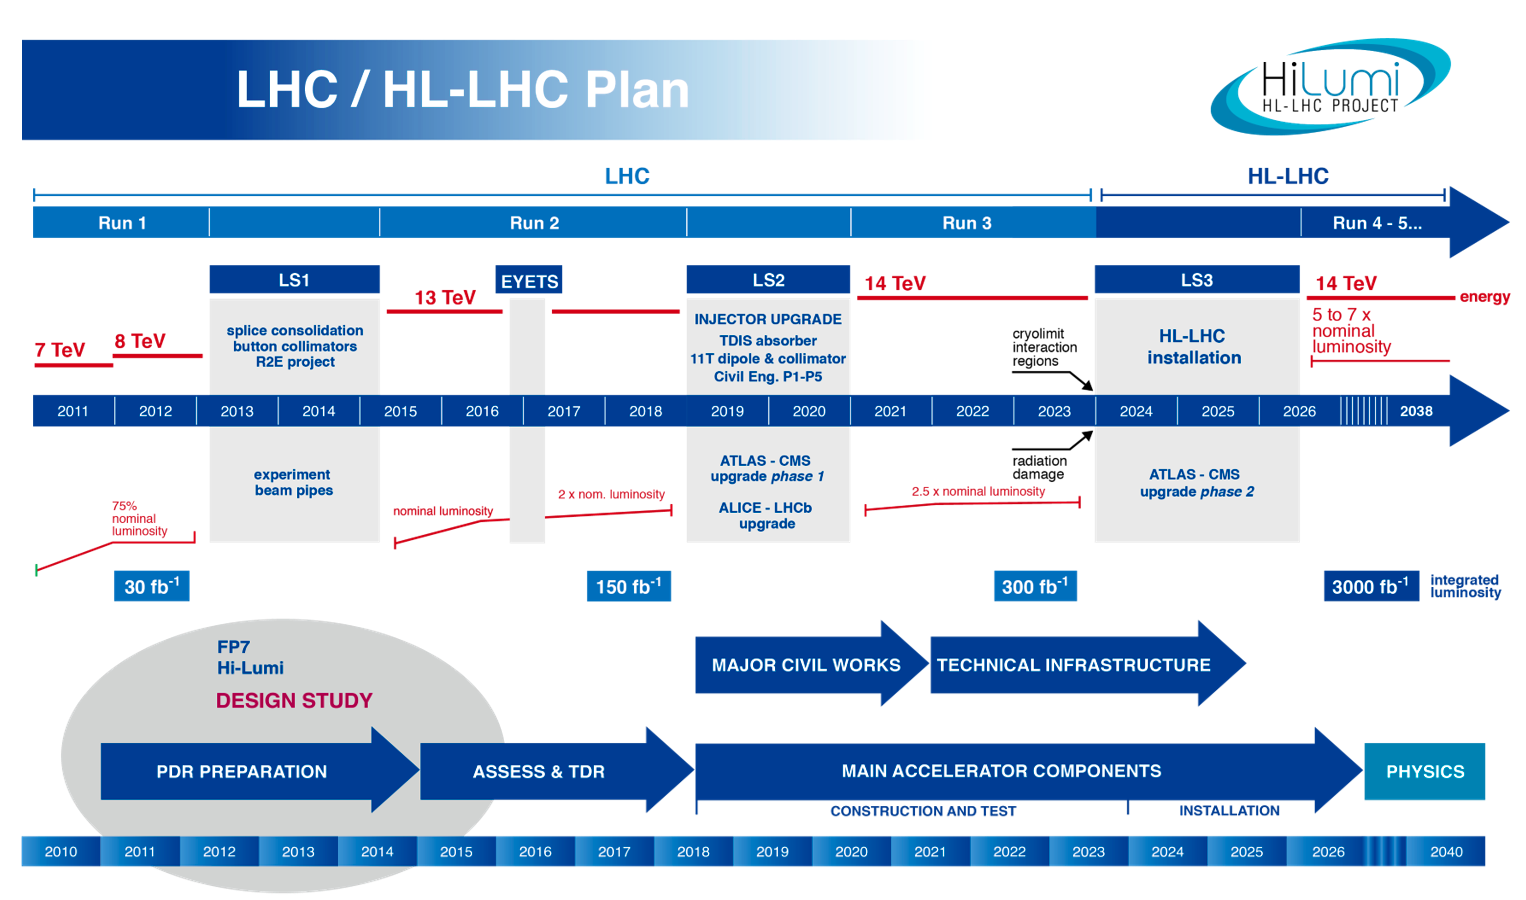
\includegraphics[width=0.9\textwidth]{Chapters/CH3/figures/phase2}
	\caption{Summary of the LHC timeline for operation and upgrade~\cite{phase2}.}
	\label{fig:phase2}
\end{figure}
\\At the end of 2018, the LHC was shut-down and for two years it will be upgraded to bring the center-of-mass energy to its design value of 14 TeV and collect 300 $\mathrm{fb^{-1}}$ of data, almost double the current available statistics of Run2.
After 4 years of duty cycle, the High-Luminosity period of LHC (HL-LHC) will start and aims to bring the integrated luminosity to 3000 $\mathrm{fb^{-1}}$, unlocking several studies, mostly related with rare phenomena, which are impossible to perform with the current datasets.\\
This chapter describes the Barrel Muon Trigger system (Section~\ref{barrel_muon_trig}), the BI upgrade for the HL-LHC (Section~\ref{BI_upg}), and the studies performed in the context of the RPC upgrade.
In particular, the goal of this work was the implementation of a new simulation to model the digitization of RPC hits in the BI region (Section~\ref{sec:hit_dig}) and, using this new model, trigger efficiency studies were performed in the BI and BM/BO regions (Section~\ref{sec:eff}).
In the end, summary and final considerations are also reported (Section~\ref{sec:concl_QT}).

\section{ATLAS Barrel Muon Trigger}
\label{barrel_muon_trig}
The muon detector chambers are arranged such that particles from the interaction point traverse three stations of chambers.\\
The system is subdivided azimuthally into 16 sectors numbered from 1 to 16.
The sector number increases in the direction of increasing $\mathrm{\phi}$ with the number 1 corresponding to coordinate $\mathrm{\phi=0}$. The odd sector (called “large sectors”)
are located between barrel coils, while, the even sectors (called “small sectors”) are covered by the coils.\\
The muon spectrometer consists of three large air-core superconducting toroidal magnets (two end-caps and one barrel) providing a field of approximately 0.5 T.\\
In the barrel, the chambers are arranged in three concentric cylinders around the beam axis called BI (Barrel Inner), BM (Barrel Middle), and BO (Barrel Outer). \\
The RPC planes are installed in the Middle
and Outer stations of the Muon Spectrometer and are mechanically associated with MDT precision chambers (except for some “special” chambers). \\
Schematic drawings of the present ATLAS MS~\cite{TDR}, are shown in Figures~\ref{fig:MS_rz} and~\ref{fig:MS_xy2}.
\begin{figure}[!h]
	\centering
	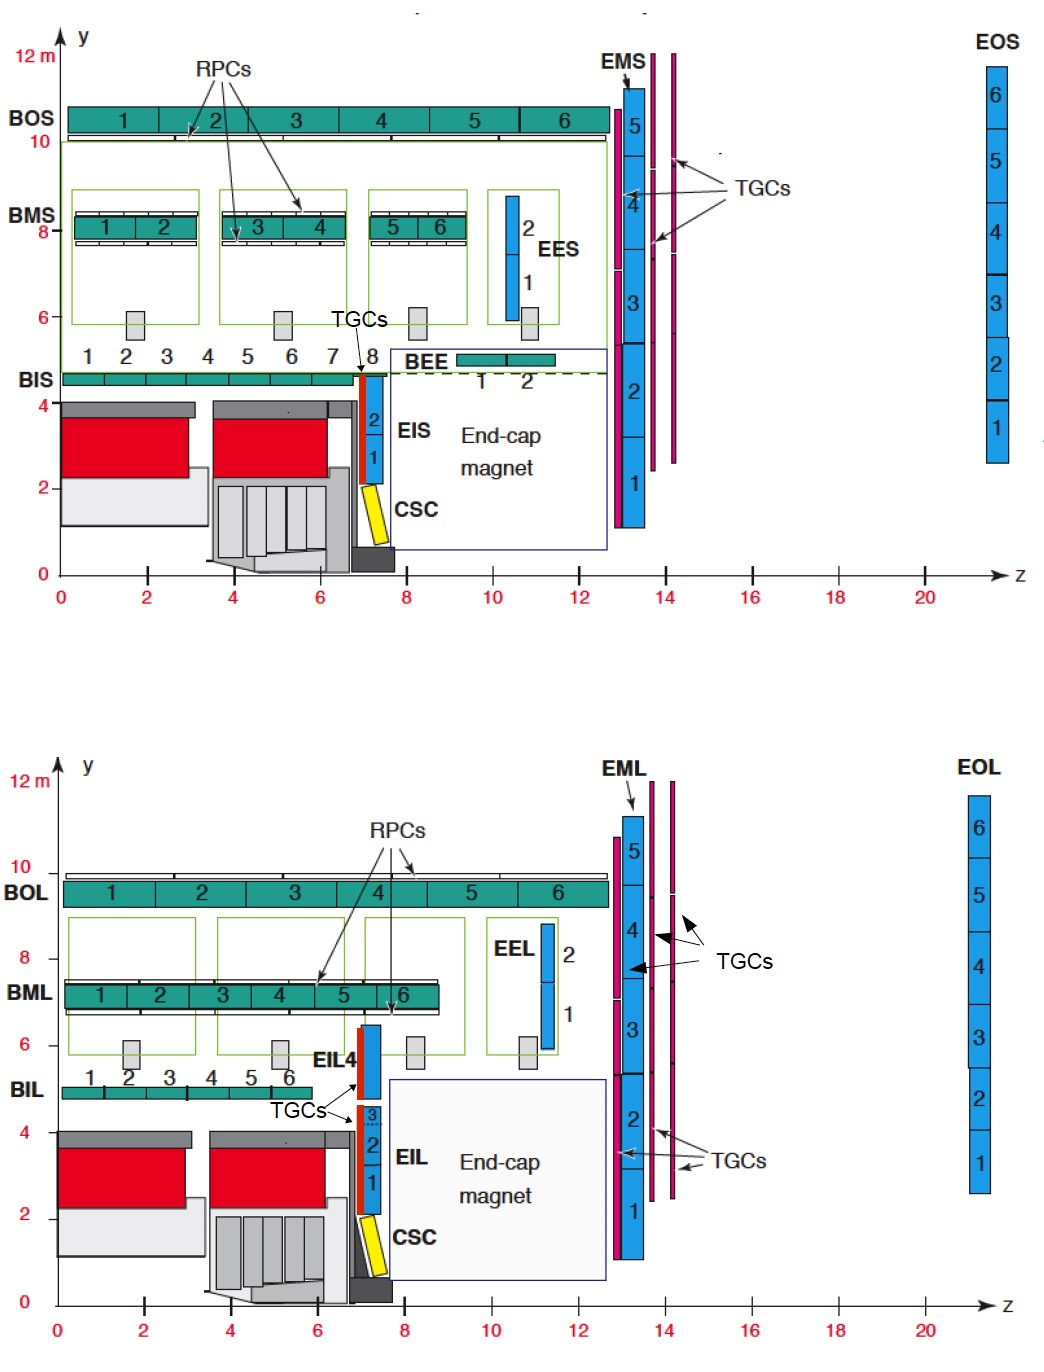
\includegraphics[width=0.9\textwidth]{Chapters/CH3/figures/MS_rz}
	\caption{Two R-Z views of the present (Run 1/2) ATLAS muon spectrometer layout. Top: One of the azimuthal sectors that contain the barrel toroid coils (small sector). Bottom: One of the sectors in-between the barrel toroid coils (large sector)~\cite{TDR}.}
	\label{fig:MS_rz}
\end{figure}
\begin{figure}[!h]
	\centering
	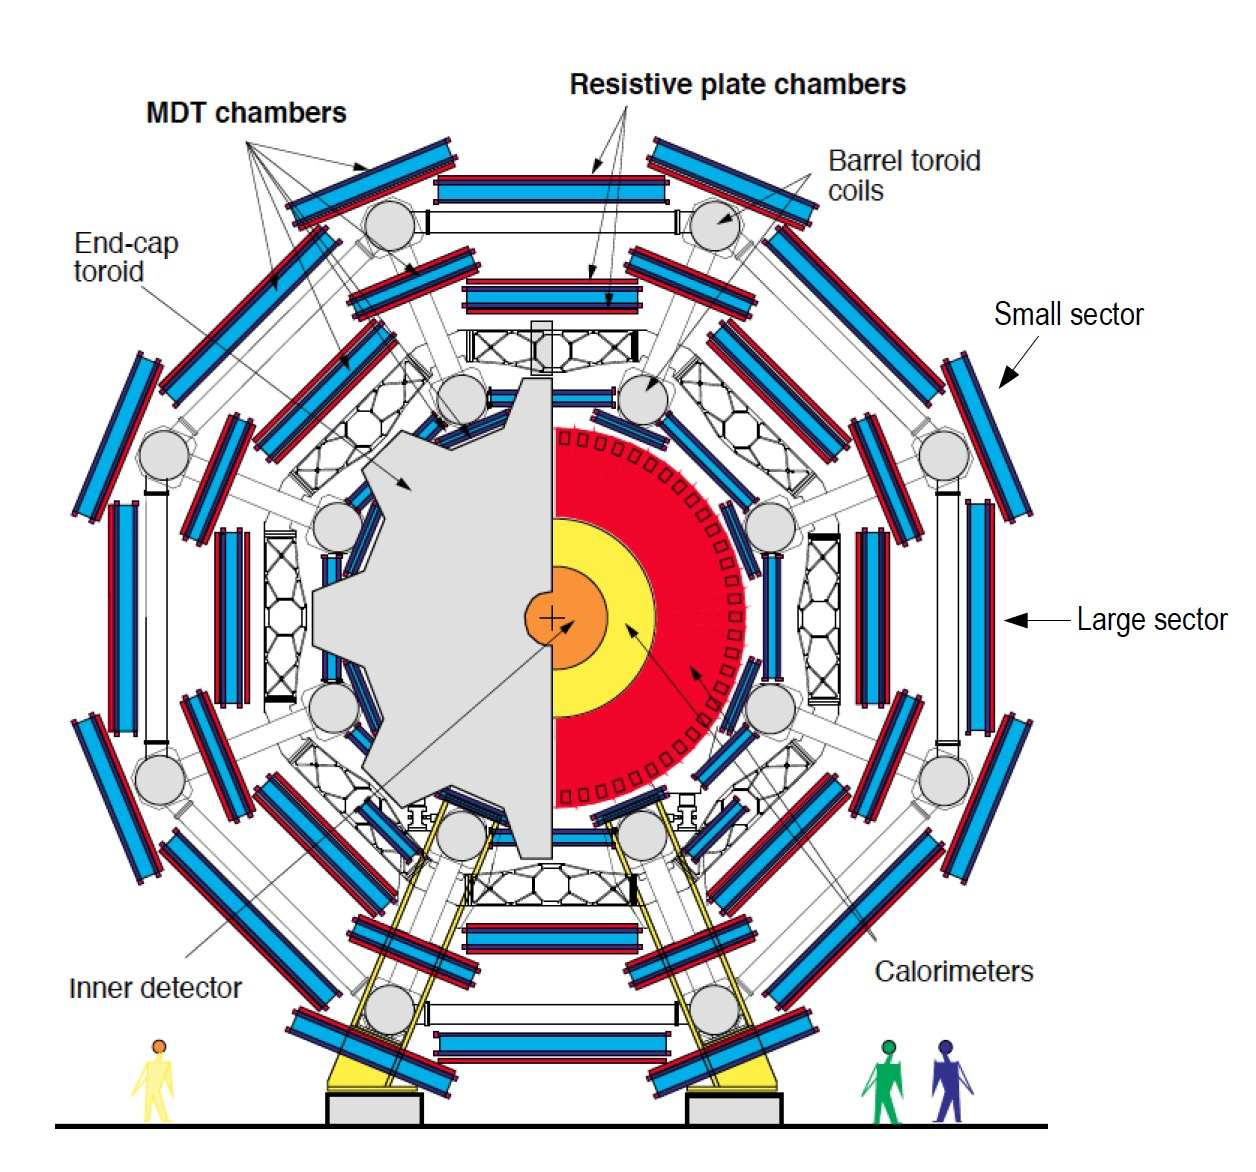
\includegraphics[width=0.9\textwidth]{Chapters/CH3/figures/MS_xy}
	\caption{View of the present (Run 1/2) ATLAS muon spectrometer barrel layout in the plane transverse to the beam axis (X-Y plane)~\cite{TDR}.}
	\label{fig:MS_xy2}
\end{figure}
The MS detector and electronics components have been designed for 10 years of operation
at a luminosity of $\mathrm{1\times 10^{34}cm^{-2} s^{-1}}$, corresponding to an integrated luminosity of 1000 \ifb. 
Conservative safety factors for radiation tolerance and rate capability were taken
into account in the original designs, and components have been tested up to and above
levels corresponding to the expected doses and rates predicted by simulations multiplied
by the safety factors. After the start of LHC operation, detector hit rates and radiation doses
could be measured directly, and the previous simulations have been found to agree with
the measurements to within a maximum deviation of about 50\%.
\\Based on this observation, the original safety factors were reduced [10], and as a consequence the original irradiation and high-rate tests have qualified the detectors for longer running and higher rates than originally anticipated.


\section {BI upgrade for Phase-II}
\label{BI_upg}
In the Phase-I upgrade, foreseen for LS2, the Small Wheels will be replaced by the New Small Wheels (NSW)~\cite{NSW} using small-strip TGC (sTGC) and Micro-Mesh Gaseous Structure
(MicroMeGaS or Micromegas, MM for short) chambers used for both triggering and precision tracking.\\
At the time of the Phase-II upgrade, there will thus be no CSC chambers
any more in the detector, nor will there be the Small Wheel MDT chambers, which are the ones closest to the beam line and exposed to the highest rates. Also in LS2, the BIS7 and
BIS8 MDT chambers will be replaced by integrated BIS78 stations of new RPC and small diameter MDT (sMDT) chambers to enhance the trigger coverage in this region~\cite{BIS78}.\\
Schematic drawings of the ATLAS MS with the new detectors that will be installed in the Phase-I and Phase-II upgrades are shown in Figure~\ref{fig:MS_rz_update}.\\
\begin{figure}
	\centering
	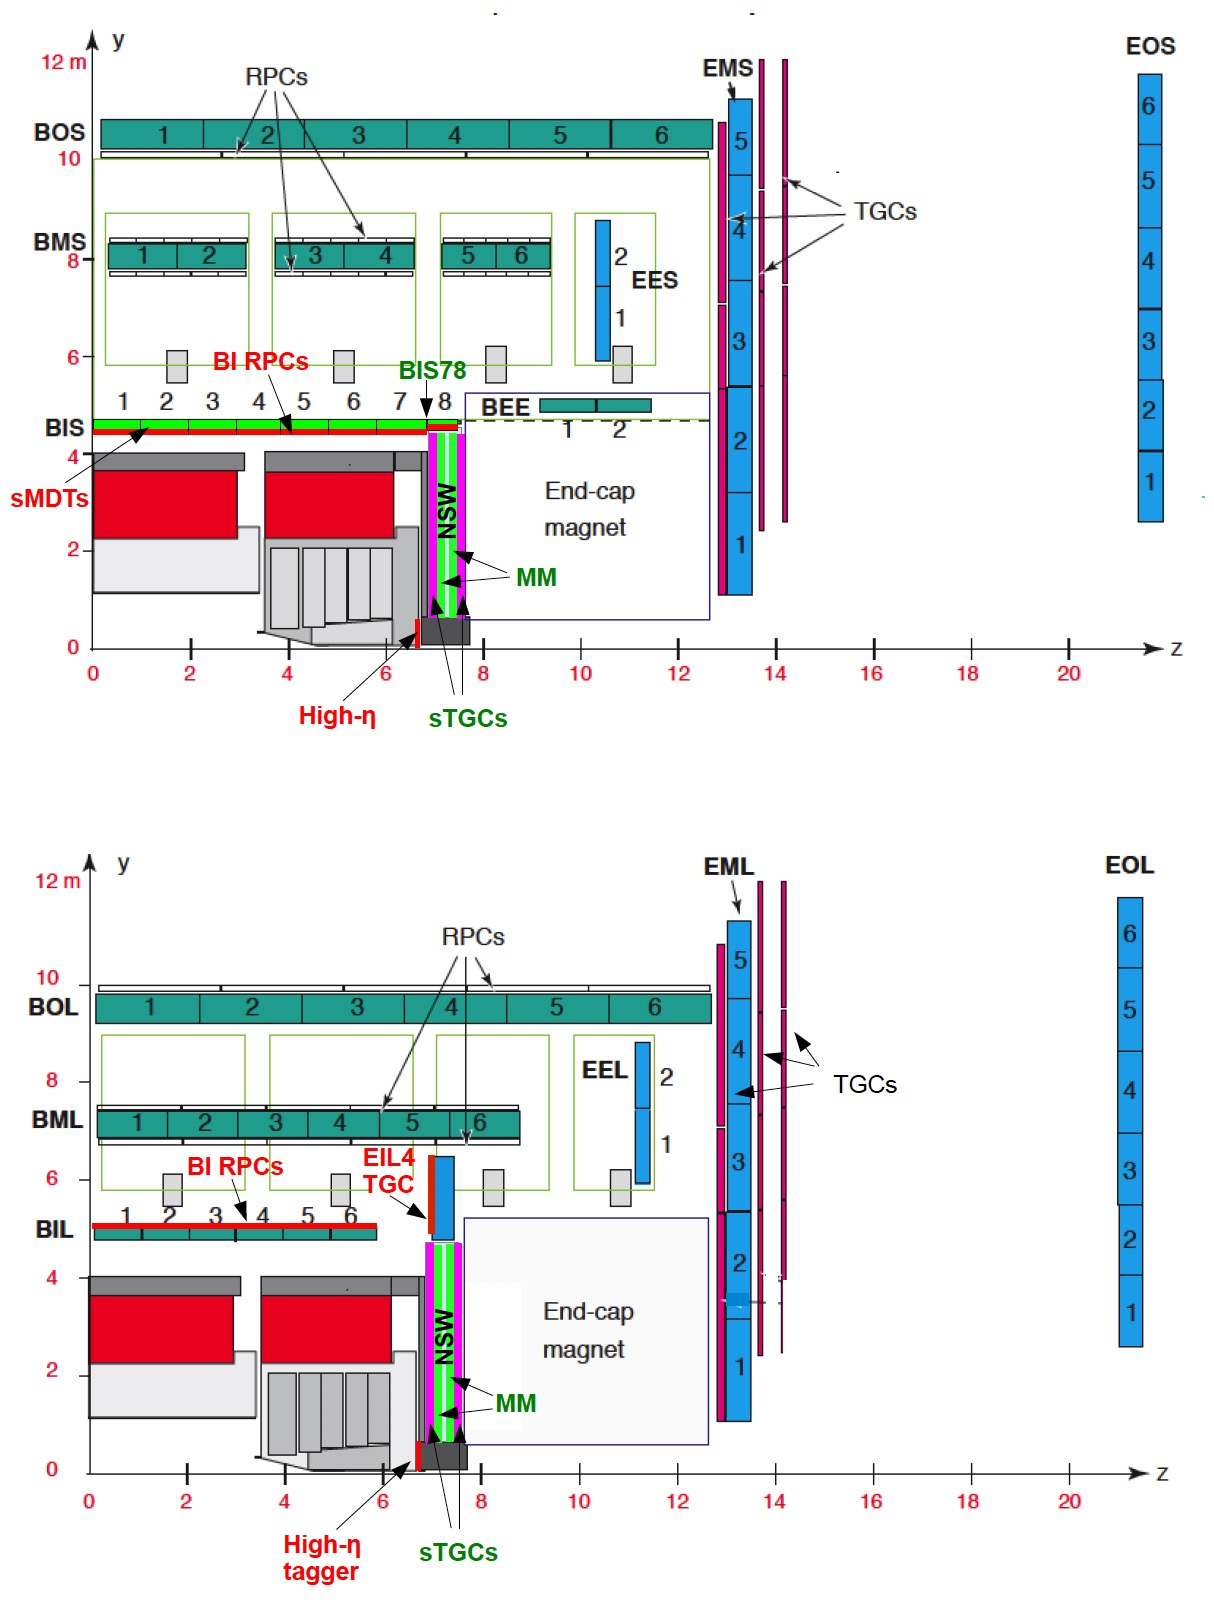
\includegraphics[width=0.9\textwidth]{Chapters/CH3/figures/MS_rz_update}
	\caption{Two R-Z views of the Phase-II ATLAS muon spectrometer layout showing a small sector (top) and a large sector (bottom). The drawings show the new detectors to be added in the Phase-II upgrade, including the addition of the high-$\mathrm{\eta}$ tagger (red text: BI RPC, sMDT, EIL4 TGC, high-$\mathrm{\eta}$ tagger), those to be installed during LS2 (green text: Micromegas and sTGC in the New Small Wheel and BIS78 RPC and sMDT), and those that will remain unchanged from the Run 1 layout (black text)~\cite{TDR}.}
	\label{fig:MS_rz_update}
\end{figure}

\noindent To maintain a high trigger efficiency, new RPC chambers with increased rate capability will be installed on the inner (BI) MDT chambers of the barrel. This addresses a fundamental issue
of the present (old) RPC chambers: to ensure their continued operation at the HL-LHC,
these chambers will have to be operated at reduced performance (i.e. efficiency), in order to
respect the original design limits on currents and integrated charge. This can be achieved
by reducing the gas gain through lowering the operating voltages. In the areas of high
backgrounds, the gas gain will have to be reduced to such low levels that hit inefficiencies
up to 35\% will be encountered. This would reduce the trigger efficiency in the barrel region
to an unacceptable level if no compensating measures were taken. In addition, due
to changes in regulations, the present gas mixture used in ATLAS RPCs may need to be
replaced by one with lower global-warming potential (GWP). Unless new gas mixtures are
found in time, this too will imply operation of old RPCs at a reduced efficiency. Despite
the lower single-hit efficiencies, a high trigger efficiency and purity can be maintained by
loosening the requirements on hit coincidences in the old chambers, if at the same time a
coincidence with the new BI RPC chambers is introduced. The installation of these chambers
will also close most of the acceptance holes of the present barrel muon trigger, which
amount to more than 20\% of the $\eta-\phi$ coverage for $!\eta!$ < 1.05 (see Section~\ref{sec:eff}).\\

\noindent Adding new RPC chambers in the barrel is challenging in terms of available space and
installation. In the small sectors, the BI RPC chambers can only be installed if the present
MDT chambers are replaced by new sMDT chambers with reduced overall thickness so that
the sMDT chambers and the new RPCs fit in the same envelope as the original MDT chambers.
In the large sectors there is sufficient space available to add the new RPC chambers
without replacing the MDTs, if on-detector services are re-arranged.\\
The retrofitting of selected RPC chambers in the BM and BO layer in the areas of high
rate at $|\eta|$ > 0.8, namely the BML7 and BOL6 chambers, is a small additional upgrade. The
MDT+RPC stations will be temporarily removed from the detector to replace the front-end
electronics and the readout panels, so that the chambers can be run at reduced HV without
efficiency loss. \\
In the Section~\ref{sec:BMBO_retrofit} it will be presented a study performed on the refurbish of
BM and BO chambers and the installation of BI chambers in the rail sectors 11 and 15.\\
The retrofitting can only be done outside the experimental cavern, on the
surface, since it requires the disassembly of the RPC chambers. The retrofitting of the BO
chambers does not fit into the LS3 schedule because it would interfere with the BI chamber
upgrade, and will likely be performed, at least partly, in winter shutdowns after LS3.\\


\noindent The main limitations of the RPC system for operation at the HL-LHC are related to the
chambers, owing to the more than a factor of seven higher luminosity than the chambers
were designed for. The RPC rate capability depends on the total charge delivered per count,
which, for the present RPCs, is 30 pC.\\
As a consequence, the single-gap efficiency will have to be reduced on average by 15\%, and by
35\% at large $\eta$. This efficiency loss will be compensated by installing a new layer of trigger chambers in the BI layer, increasing the overall barrel trigger redundancy.\\
To operate reliably at the HL-LHC, with high acceptance and efficiency and maintaining, the high trigger selectivity of the present system, several upgrades are required for the RPC system:
\begin{itemize}
	\item A new inner layer of BI RPC chambers will be added to the spectrometer. This will
recover most of the current geometrical acceptance holes. The redundancy of the
system will be greatly enhanced, so that full trigger efficiency can be maintained even
if the old RPCs have to be operated at reduced efficiency, either to limit the effects of
ageing or because the use of a different gas mixture is enforced. The BI RPCs will be
new-generation RPCs with 1 mm gas gaps and high-sensitivity front-end electronics.
	\item The trigger and readout electronics (Pad and splitter boxes) have to be replaced in order
to make the RPC system compliant with the Phase-II ATLAS trigger and readout
scheme. The entire electronics chain, except for the front-end boards, will be replaced.
The Pads will be replaced by the new data collector and transmitter (DCT) boards that
will send all data off the detector to the counting room USA15 where the trigger and
readout logic will be performed.
	\item In a worst-case scenario for the required reduction of efficiency of the old RPCs, a
reduction of the trigger efficiency may still occur even after the BI RPC installation,
in the region of $|\eta|$ > 0.8. This efficiency loss can be recovered by retrofitting a limited
number of BO chambers in that region. The retrofitting comprises replacing the
original front-end electronics by the new BI version, and replacing the readout strip
panels.
\end{itemize}
\newpage
\subsection{RPC upgrade}
The BI system is designed to increase the trigger acceptance and the trigger efficiency, by
loosening the requirements on the number of hits in the BM and BO chambers and, at the
same time, adding the requirement of a coincidence with the BI layer. Any coincidences of
hits in at least three chambers out of four (counting one BI, two BM, and one BO) will be
accepted. Two-chamber BI-BO coincidences will be used to cover the remaining acceptance
holes. Details of the Phase-II trigger algorithms and their performance are discussed in
Section~\ref{sec:trigScheme}. Figure~\ref{fig:tdr_eff} illustrates the recovery of acceptance and 
efficiency obtained with the Phase-II trigger including the BI RPCs in a worst-case scenario in 
which the single-hit efficiency of the old RPC is reduced by 15–35\% as a function of $|\eta|$, 
depending on the rate to which each chamber is exposed.
\begin{figure}[!h]
	\centering
	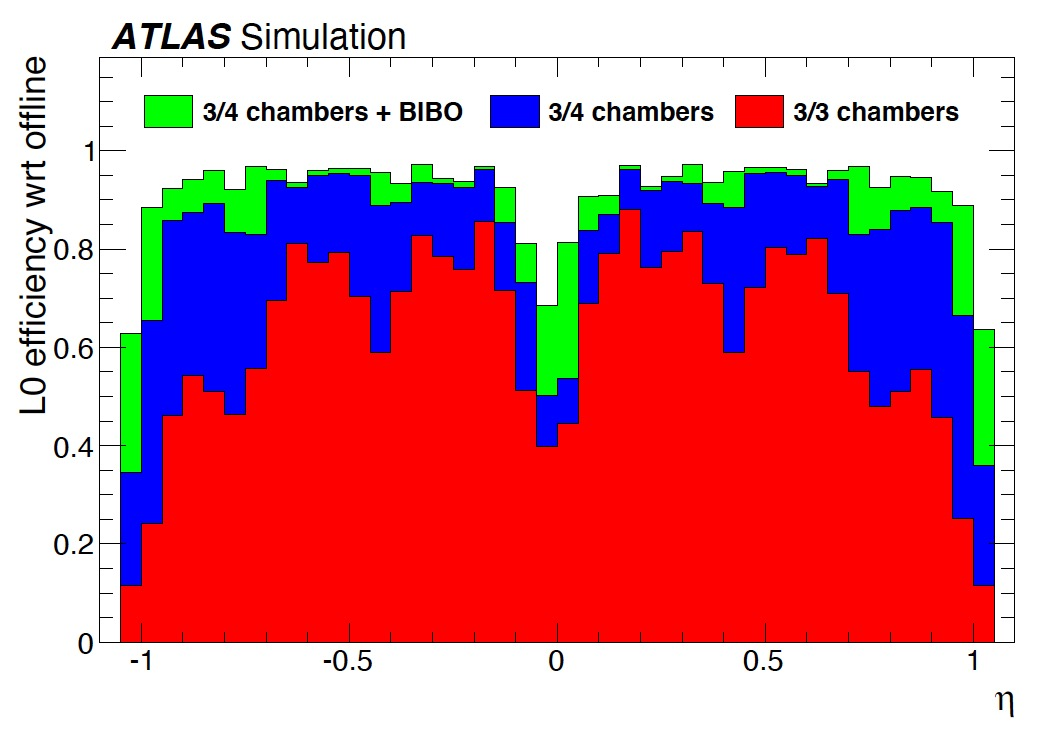
\includegraphics[width=0.9\textwidth]{Chapters/CH3/figures/tdr_eff}
	\caption{Efficiency times acceptance of the L0 barrel trigger for reconstructed muons with $p_{T} =
     25$ GeV as a function of $\eta$, assuming the worst-case scenario~\cite{TDR}.}
	\label{fig:tdr_eff}
\end{figure}
\\The new BI RPC chambers will have three sensitive gas gaps that are read out independently.
A majority logic requiring hits in at least two out of three planes provides high efficiency
while suppressing the rate of random coincidences due to uncorrelated hits from
photons and neutrons. This is necessary, for instance, to keep the rate of BI-BO coincidences
at an acceptable level.\\
A major re-design of the RPC technology started around the year 2010, mainly aiming at a
better rate capability and ageing behaviour. The new design is based on a reduced thickness
of the gas gaps (from 2 mm to 1 mm) and of the resistive electrodes (from 1.8 mm to
1 mm), and on the use of a new generation of low-noise high-sensitivity amplifiers. Using
these amplifiers, full efficiency can be achieved for a lower voltage across the gas gap, thus
transferring part of the amplification from the gas avalanche to the electronics. In this way,
the RPCs can be operated at a reduced charge per avalanche, reducing the detector current
and thus improving rate capability and ageing.\\
A detail view of the positions of the BI RPCs in ATLAS is shown in Figure~\ref{fig:xy_BIRPC}.
\begin{figure}[!h]
	\centering
	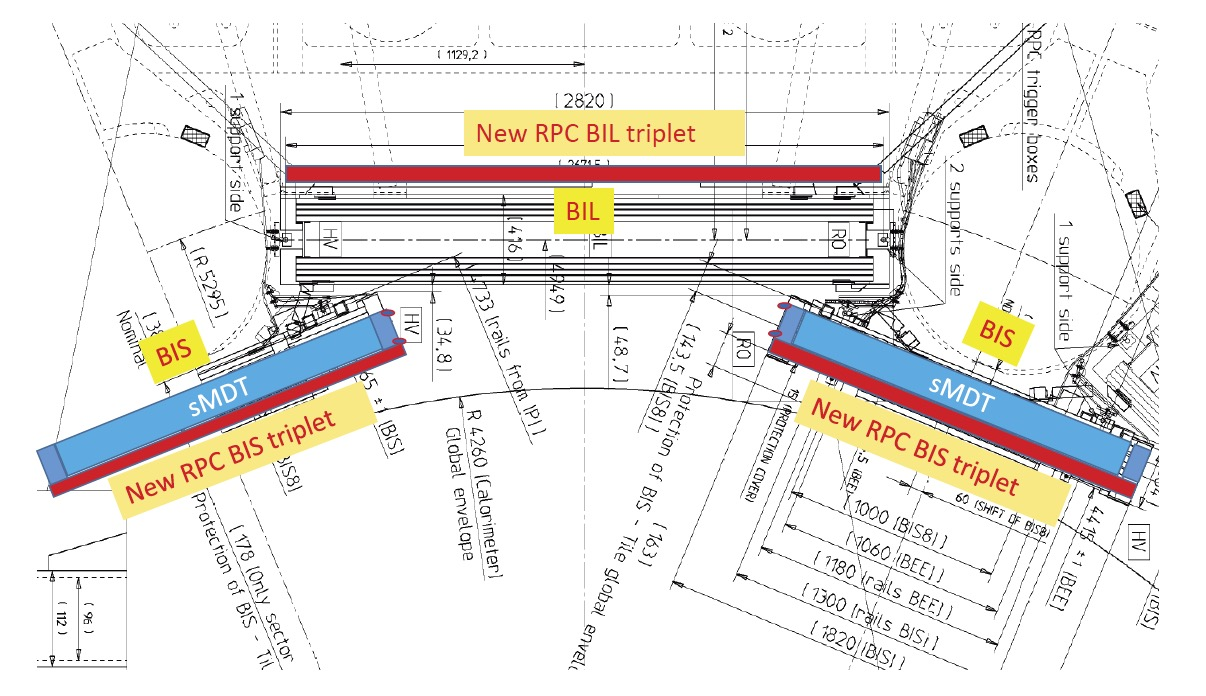
\includegraphics[width=0.9\textwidth]{Chapters/CH3/figures/xy_BIRPC}
	\caption{X-Y view of the inner barrel layer, indicating the positions of the BI RPCs (red) and BIS
sMDTs (blue) in the small and large sectors~\cite{TDR}.}
	\label{fig:xy_BIRPC}
\end{figure}
\\In the small sectors (BIS), due to the tight space limitations, the MDT chambers need to be 
replaced by new small-diameter MDT (sMDT) chambers with half the tube diameter (15 mm 
instead of 30 mm) in order to create space for the RPCs on the inside of the sMDT chambers. 
In  the large sectors (BIL), the new RPCs will be installed on the outside of the existing MDTs. The
layout of the new BI RPCs leaves the necessary holes and cut-outs for the existing MDT
alignment lines and for detector services. It comprises 272 triplet RPC chambers, for a total
area of about 470 $\mathrm{m^{2}}$. Acceptance studies based on a realistic description of the BI RPC geometry show a geometrical acceptance of the BI RPC chambers of 91\% for reconstructed muons with $|\eta|$ < 1.05, compared to 95\%  for the MDT chambers. This results in a barrel trigger acceptance of 96\%.\\
Each detector layer of the triplets is read out on both surfaces by orthogonal strip panels,
providing $\eta$ and $\phi$ measurements. The compact triplet structure and the use of highly
sensitive amplifiers require a complete isolation of individual layers from each other. The
choice of strip pitches, 24–26 mm depending on the chamber type, has been constrained
by the performance requirements, the strip impedance, and cost considerations. The total
number of readout channels is about 8700.

\subsection {Trigger scheme}
\label{sec:trigScheme}
All the hits from RPC detectors will be available to the barrel Sector Logic board that uses them to
generate barrel trigger candidates. The new BI RPCs increase the geometrical acceptance
of the present barrel muon trigger and its robustness against inefficiencies of the old BM
and BO RPCs caused by the reduced operating voltages necessary to ensure their longevity.\\
The RPC trigger will use nine measurement planes, provided by four layers of RPC chambers:
one BI triplet (RPC0), two BM doublets (RPC1 and RPC2), and one BO doublet (RPC3).
Figure~\ref{fig:trig_schemeXY} shows the positions of the BI, BM, and BO RPC chambers in a small 
barrel sector
together with the MDT chambers. The acceptance holes in the BM layer, caused by the
magnet coils and their supports, are also visible.
\begin{figure}[!h]
	\centering
	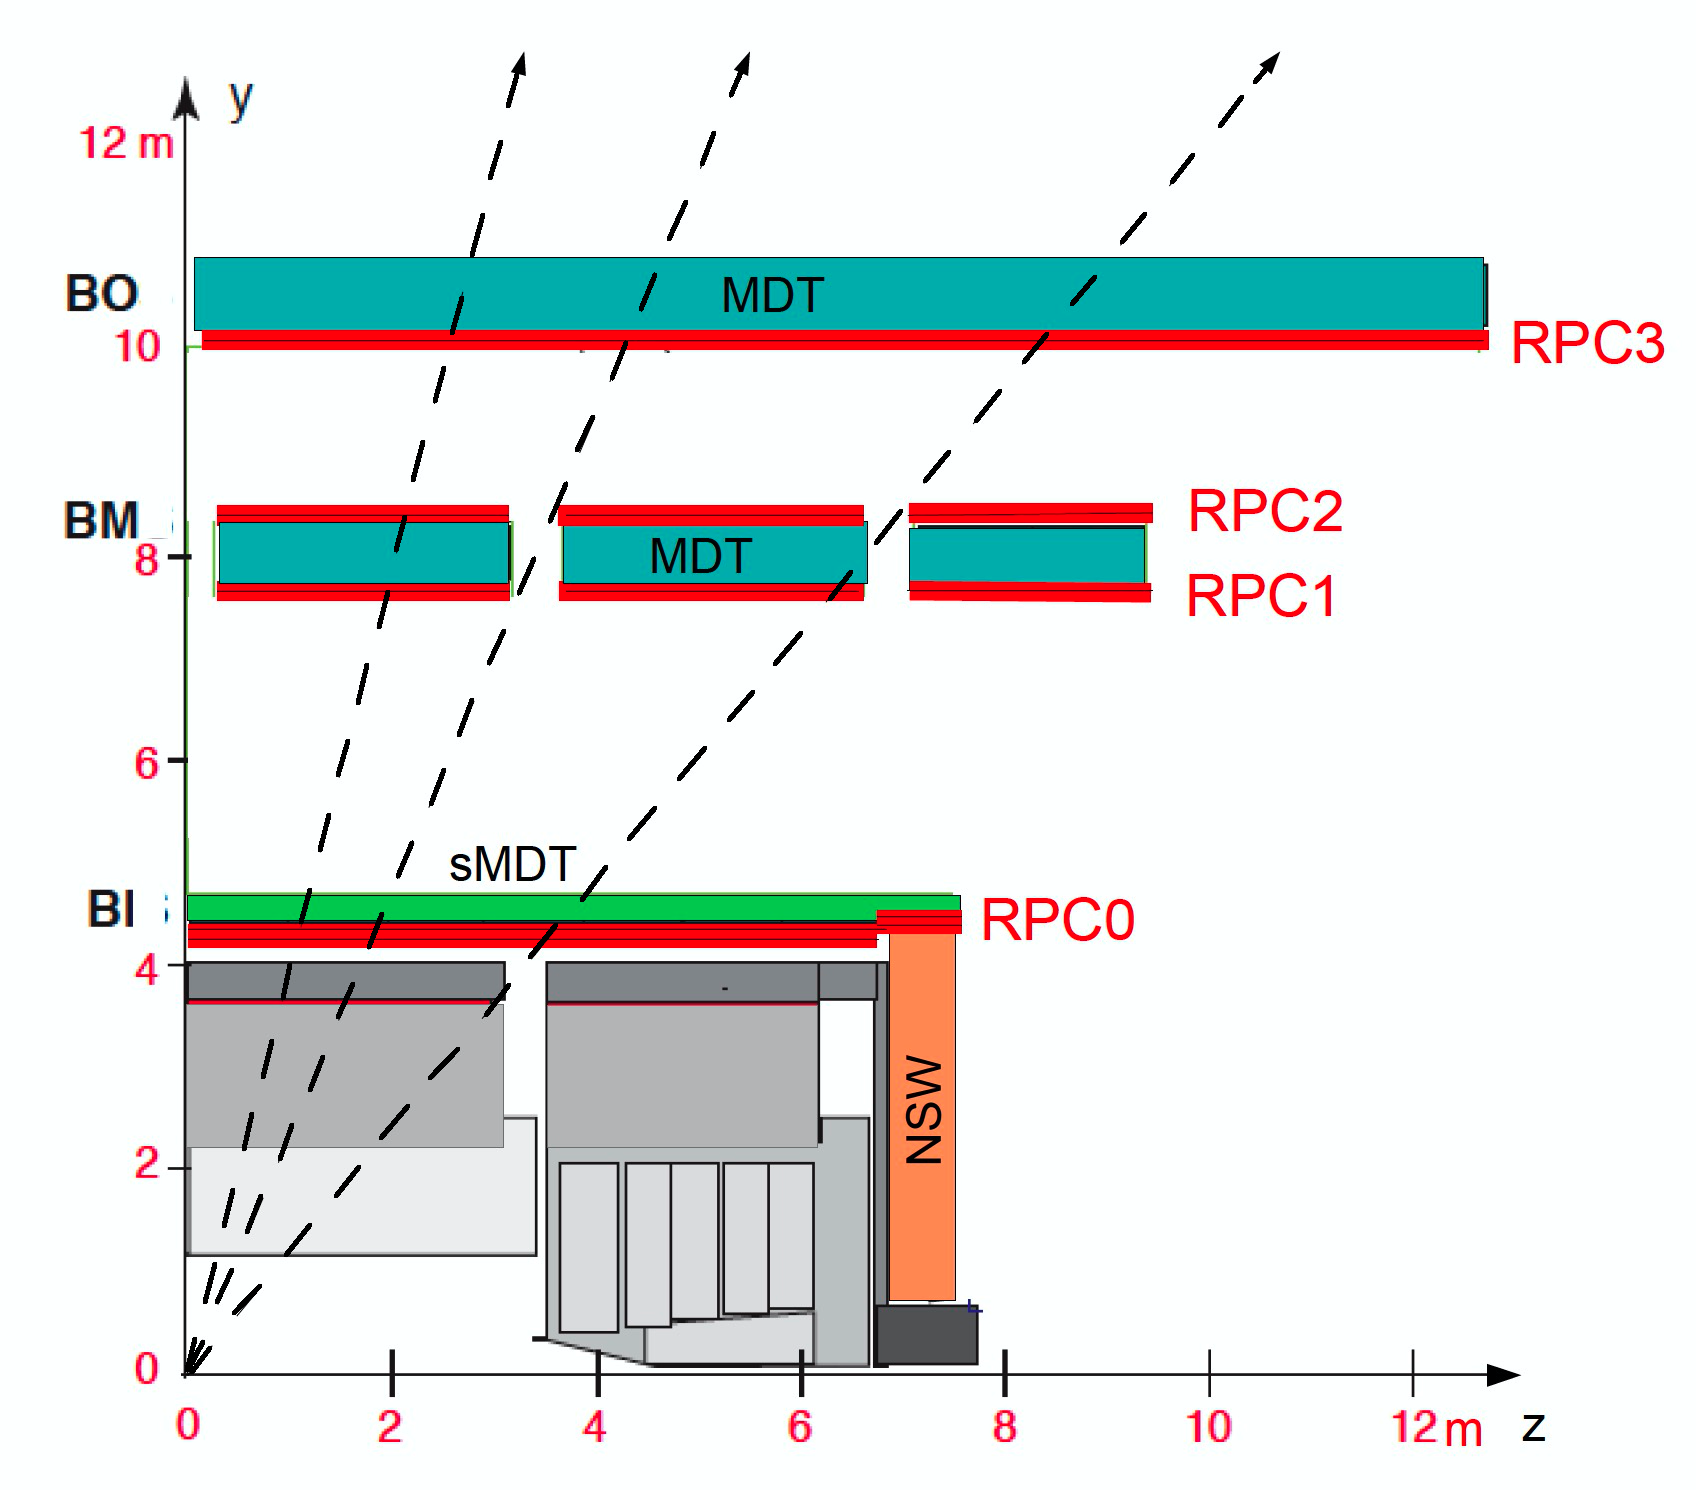
\includegraphics[width=0.75\textwidth]{Chapters/CH3/figures/trig_schemeXY_paint}
	\caption{Transverse section of a small sector in the barrel region, showing the four layers of RPC chambers (RPC0,1,2,3), as well as the MDT chambers in the barrel-inner (BI), barrel-middle (BM), and barrel-outer (BO) layers. The three dashed lines represent muon trajectories traversing four, two, and three RPC chambers~\cite{TDR}.}
	\label{fig:trig_schemeXY}
\end{figure}
\\To take advantage of the redundancy of detector planes, a trigger algorithm that does not
make use of a fixed pivot plane (as in present ATLAS muon trigger) has been developed.
This makes it possible to define different trigger coincidence logic schemes.\\ 
These schemes (summarised in Table~\ref{tab:trig_scheme} and illustrated in Figure~\ref{fig:trig_scheme}) are based on different requirements on the  four layers of RPC chambers:
\begin{itemize}
	\item 3/3 chambers. Hits in at least three out of four planes of the RPC1+RPC2 chambers
and in at least one out of two planes of RPC3. This is equivalent to the present high-pT
trigger.
	\item 3/4 chambers. The previous requirement in a logical OR with the requirement of
hits in at least two planes out of three in RPC0 and in at least three planes out of six
in RPC1+RPC2+RPC3. In this way, all combinations of three-chamber coincidences
(satisfying the above hit requirements) are accepted.
	\item 3/4 chambers + BI-BO. The previous requirement in a logical OR with the requirement
of at least two hits in RPC0 and at least one hit in RPC3. This enhances the
trigger coverage in the regions where no BM RPCs are installed due to the mechanical
support structure of the toroid coils. The BI-BO coincidence is expected to be
prone to accidental coincidences of uncorrelated background hits that are negligible
in three-chamber coincidences. In the baseline version of this trigger, BI-BO coincidences
are used in the whole barrel region, but can be limited to the BM acceptance
gaps, if the muon trigger rate in the barrel gets too high.
\end{itemize}
\begin{table}[h]
	\begin{center}
		\begin{tabular}{lp{0.75\textwidth}}
			\textbf{Trigger}  & \textbf{Requirement} \\
			\hline 
			3/3 chambers     & \scriptsize{\texttt{3[RPC1+RPC2] AND 1[RPC3]}} \\
			3/4 chambers     & \scriptsize{\texttt{(3[RPC1+RPC2] AND 1[RPC3]) OR (2[RPC0] AND 3[RPC1+RPC2+RPC3])}}\\
			3/4 ch.+BI\&BO    & \scriptsize{\texttt{(3[RPC1+RPC2] AND 1[RPC3]) OR (2[RPC0] AND 3[RPC1+RPC2+RPC3]) \hspace{2cm} OR (2[RPC0] AND 1[RPC3])}}\\
			\hline 
		\end{tabular} 
		\caption{The hit requirements used in different RPC triggers. The left column shows the short name used in the text. The right column gives the coincidence scheme used for the selection logic. The notation \texttt{N[RPCi+RPCj+...]} indicates a majority requirement of hits in at least N planes out of all the possible planes available in RPC chambers RPCi, RPCj, . . . with \textit{i, j,} . . . \textit{$\in$} $\{0, 1, 2, 3\}$.} 
		\label{tab:trig_scheme}
	\end{center} 
\end{table} 
\begin{figure}[!h]
	\centering
	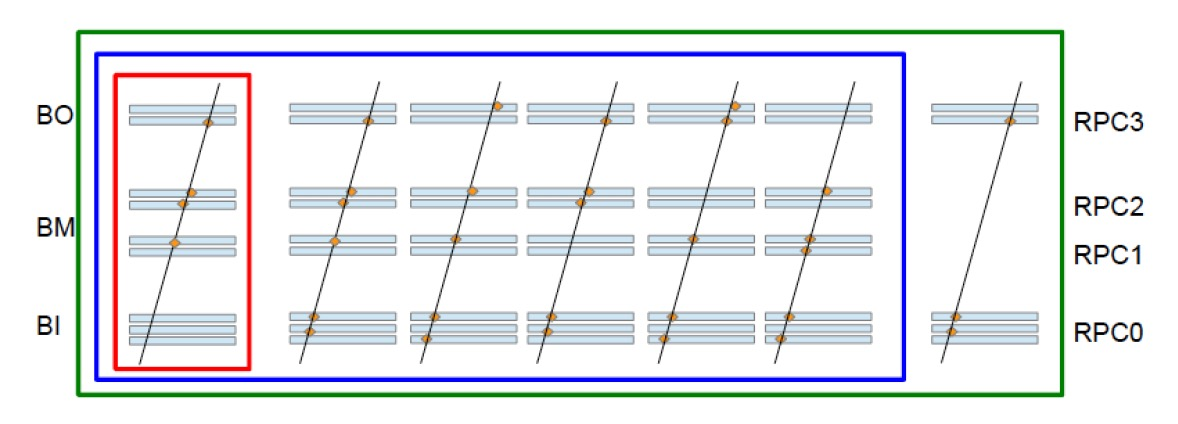
\includegraphics[width=0.8\textwidth]{Chapters/CH3/figures/trig_scheme}
	\caption{Graphic view of the coincidence scheme used for the selection logic. High-Pt (3/3 chambers) in red, 3/4 chambers in blue, 3/4 ch.+BI\&BO in green.}
	\label{fig:trig_scheme}
\end{figure}

\section{Hit digitization in the BI region}
\label{sec:hit_dig}
Since at the present time the new chambers in the BI region are not yet installed,
the simulation performed for this work takes into account the presence 
of hits in the BI RPC chambers exploiting the true hits, recorded 
by the MDT chambers in the BI region, and treating them as hits of the future RPC chambers.\\
In this work, it has been used the the common framework \texttt{muTrigNt\_write}~\cite{muTrigNt} that includes a realistic digitization.
This code reproduces the dimensions of the new BI RPC chambers and, 
given as input the true MDT hits, it checks if the hits are in the geometric 
acceptance.
The code also allows to generate strips, of an arbitrary pitch, in the two orthogonal directions ($\eta$ and $\phi$) and thus to digitize the true MDT hits, recording them as hits with the coordinates reported in the center of the strip.
In this way, it is possible to completely simulate the RPC chamber. \\
%This \texttt{muTrigNt\_write} is also able to simulate the trigger efficiencies, as described in Sec~\ref{sec:eff}. 
The studies presented in this chapter were performed using the official MC sample\\  {\scriptsize\texttt{mc15\_14TeV.422063.ParticleGun\_single\_mu\_Pt50.recon.ESD.e5392\_s2988\_s3000\_r8974}}~\cite{Muontwiki}, containing 50K events, produced with the ITk (Inner Tracker) simulation and with the layout of Run-I muons, that differs compared to the layout of Run-II muons because the feet and the elevator chambers are missing.
This MC sample considers muons reconstructed in $|\eta| < 1.05$ by the offline reconstruction, using a single-muon MC sample with fixed \mbox{$p_{T}=50$ \GeV}. \\
Given the framework described above, the goal of this work was to implement a simulation with a more realistic digitization that would produce:
\begin{itemize}
	\item cluster size, strip number and the associated coordinates of the strips (Section~\ref{sec:CSM});
	\item timing (Section~\ref{sec:timing});
	%\item the option of BI RPCs with two-sides $\eta-\eta$ readout  (Section~\ref{sec:etaeta});
%	\item BI and BMBO Efficiencies (Section~\ref{sec:eff});
\end{itemize}

\subsection{The cluster size model}
\label{sec:CSM}
A single discharge in the gas volume can induce a signal in more than
one RPC strip (i.e. it causes a so-called $cluster$), which is due to the charge sharing.
The number of the RPC strips fired in temporal coincidence is called $cluster$ $size$. 
The cluster size is a relevant parameter for the RPC detector and it must be strictly monitored to 
ensure a full trigger efficiency,
The cluster size is simulated using a Gaussian charge distribution, with fixed width and centered on the true MDT hit that is induced on the strips~\cite{MuonWeek22Oct}. 
This function is defined as:
\begin{equation}
G(z)=A(z)\cdot \frac{2}{\pi} \int{e^{-\frac{\mu-z}{\sigma\sqrt{2}}}}
\end{equation}
where the amplitude $A(z)$ is a random distribution having a decreasing exponential distribution  $f(A)=e^{-\frac{z}{\tau}}$, with the parameter $\tau$ = 0.8, fixed width $\sigma$ = 16 mm and $\mu$ is the $z$~-~coordinate of the hit.
When the charge integrated over a strip exceeds a certain threshold (0.2 in this simulation), the strip is switched on.\\
This is not a strictly physical model but a decreasing exponential is useful to produce the expected tail, in the absence of a more realistic model for amplitudes
based on experimental studies. A picture of the model used in this simulation is illustrated in Figure~\ref{fig:csm_pic}.
\begin{figure}[!h]
	\centering
	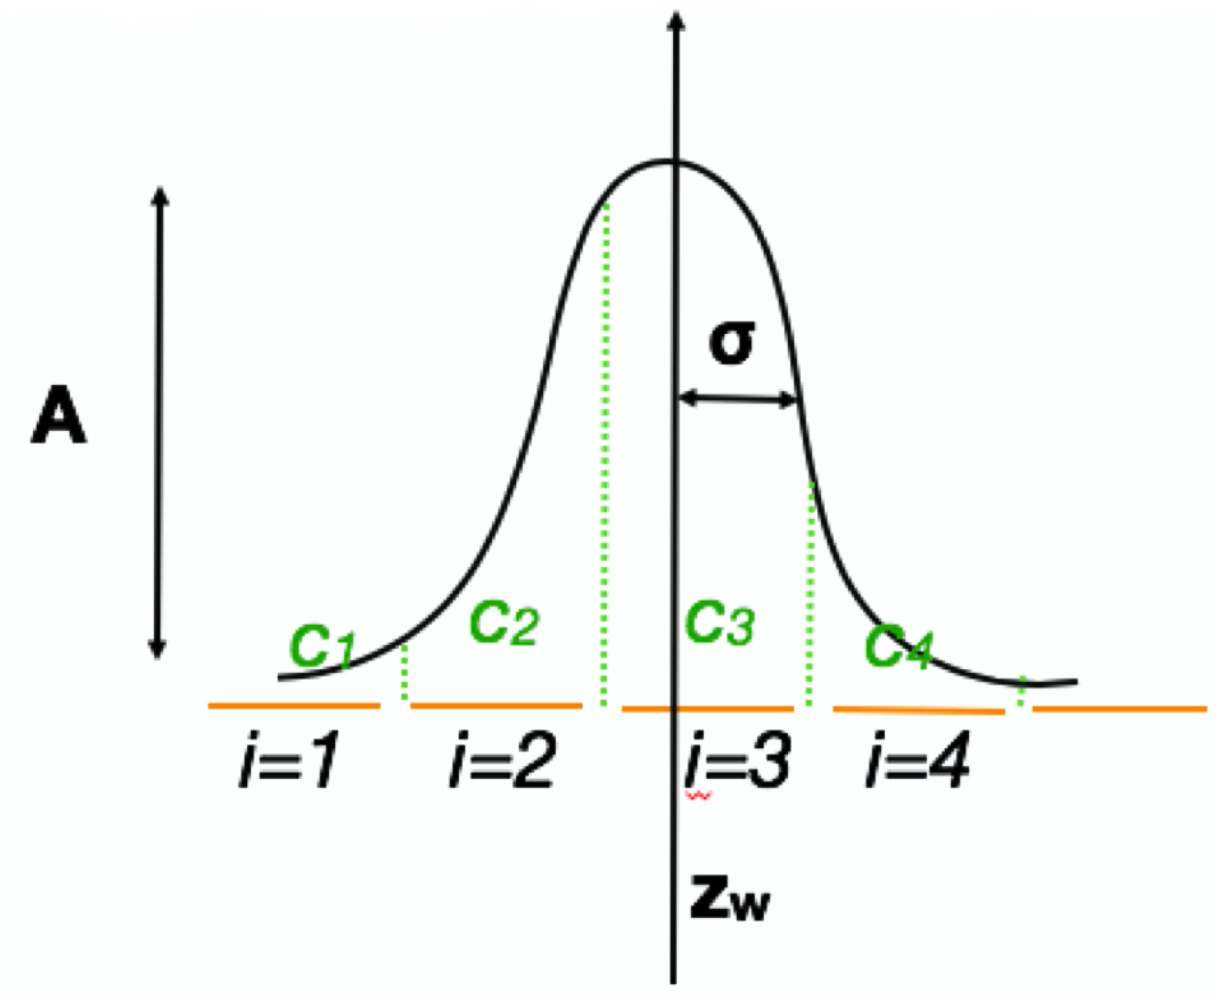
\includegraphics[width=0.53\textwidth]{Chapters/CH3/figures/csm_pic}
	\caption{Cluster size model used in the simulation. $C_i$ is the charge integrated over a strip $i$. 
		Some other parameters are the strip pitch $z_w$ ( 22 mm), random amplitude$A$ and width $\sigma$. When the charge integrated over a strip exceeds a certain threshold, the strip is switched on~\cite{MuonWeek22Oct}.}
	\label{fig:csm_pic}
\end{figure}
Cluster size is given by the number of strips fired at the same time. \\
It depends on the absolute value of charge integrated over a strip, but it also depends on the position of the true hit.
Originally, the RPC hit is fixed to be at the center of the strip and the true MDT hit belongs to one strip only but in this simulation, it would be possible to have many strips fired at the same time using the relation: $\mathrm{GlobPos_{i} = GlobPos_{i,true}\pm strip\_center_{i}}$. 
The resulting cluster size distribution is in line with the expectations in~\cite{TDR} and shown in Figure~\ref{fig:CS}.
\begin{figure}[!h]
	\centering
	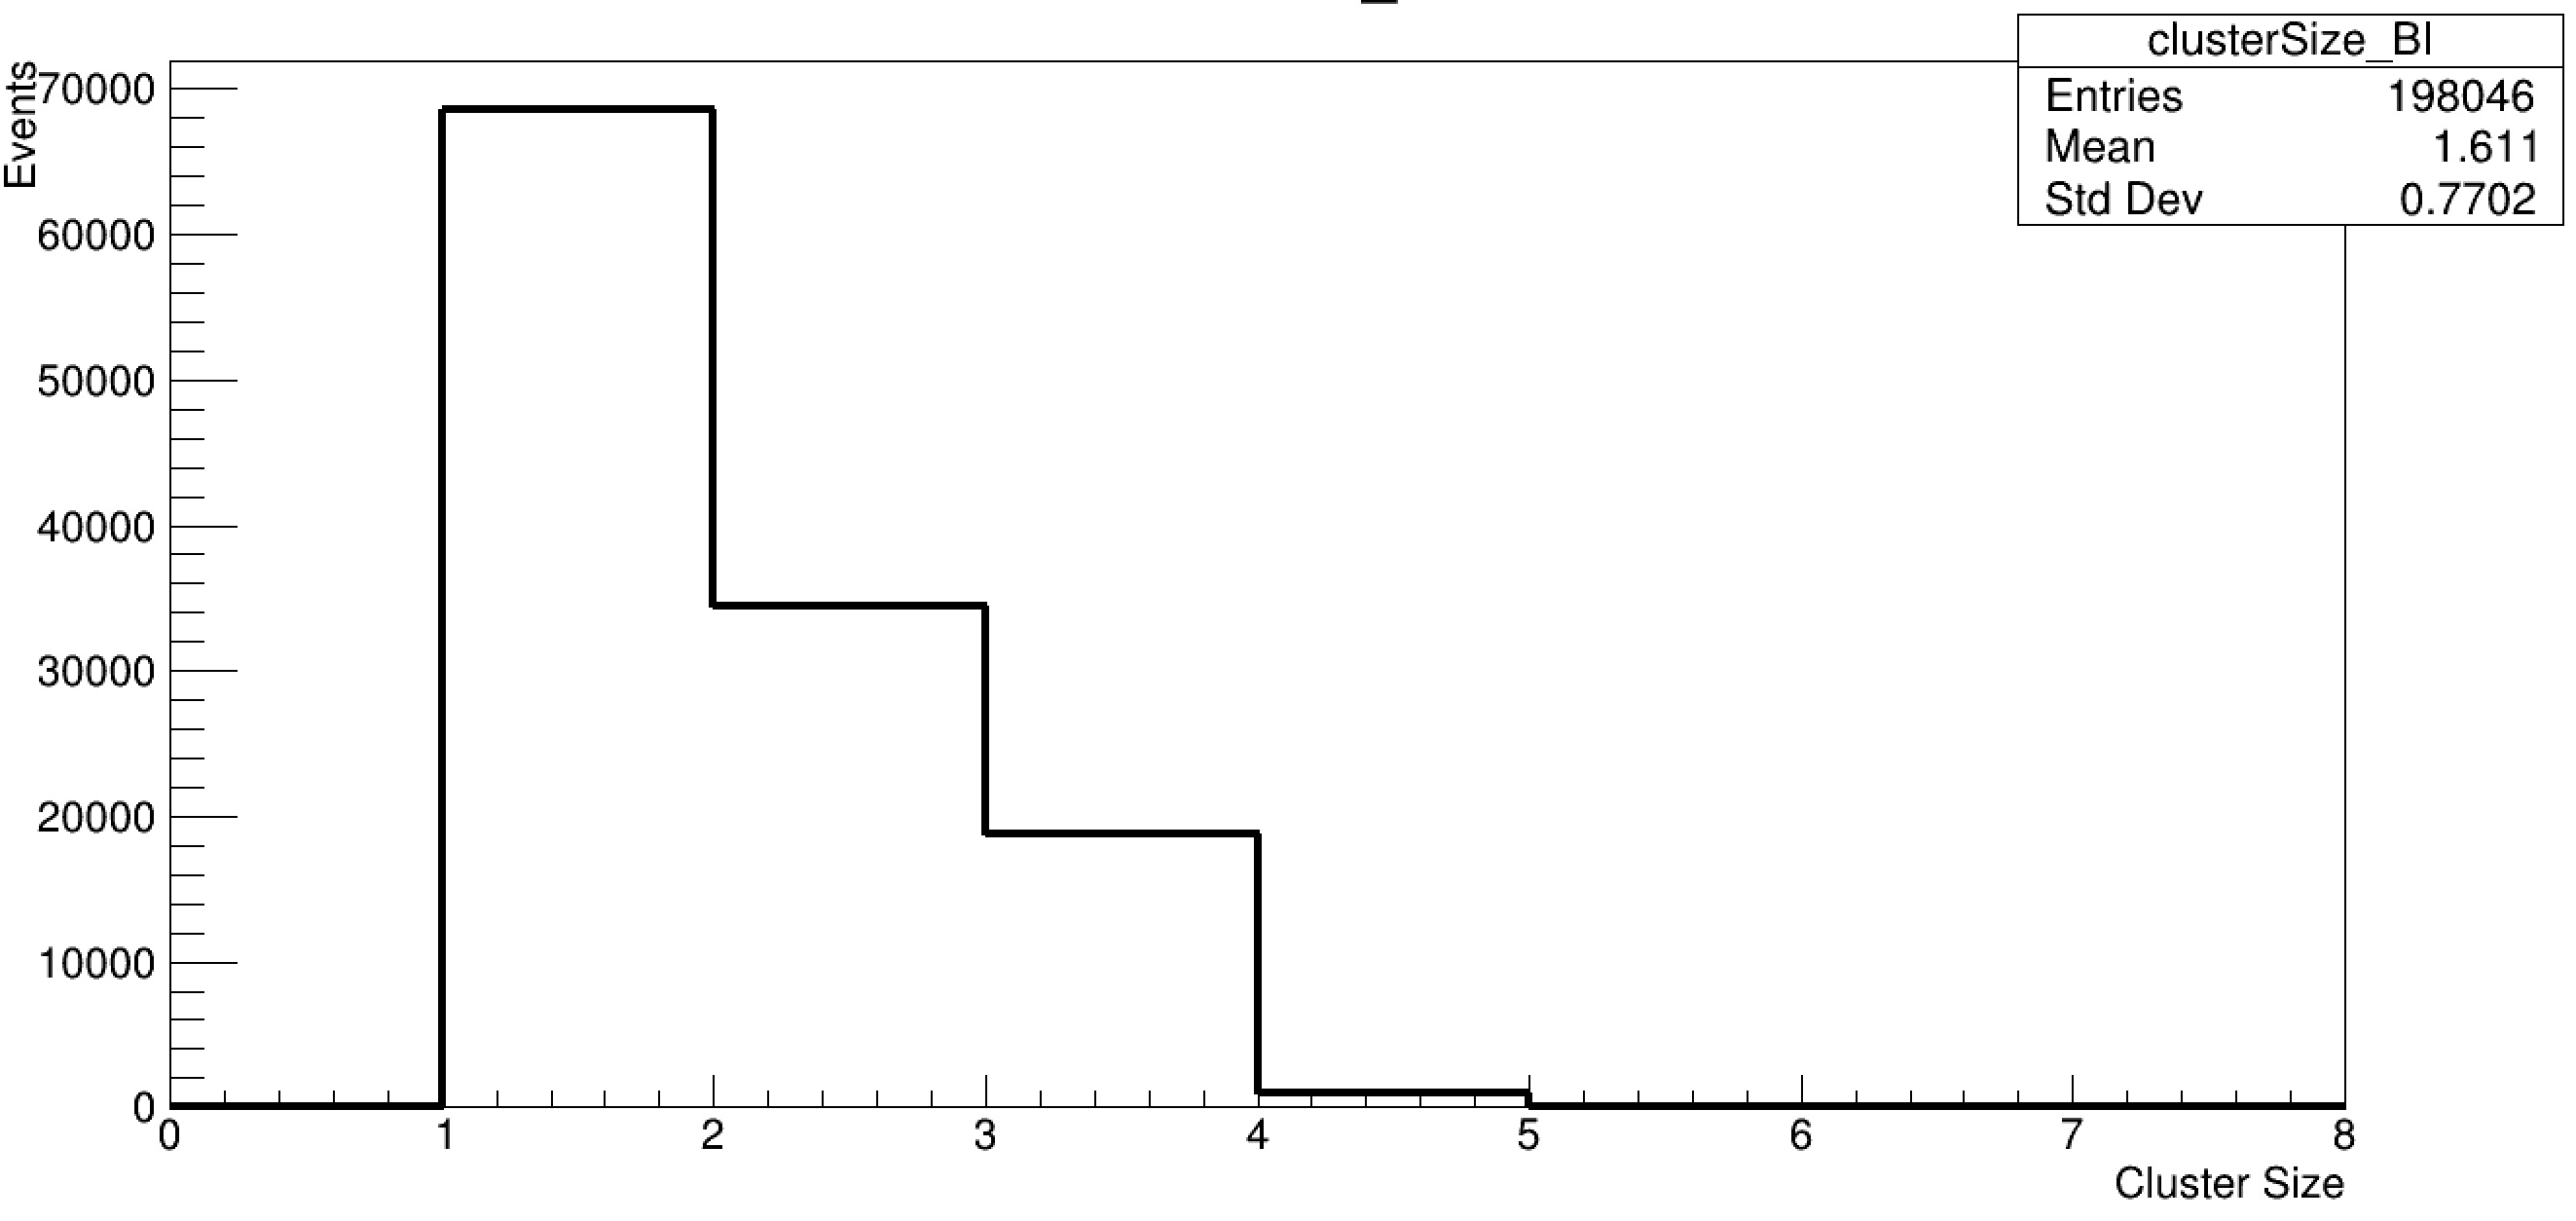
\includegraphics[width=0.7\textwidth]{Chapters/CH3/figures/CS}
	\caption{Cluster size distribution obtained with the model and parameters illustrated in this section. The average value is 1.6.}
	\label{fig:CS}
\end{figure}
\newpage\phantom{}
\noindent Considering the hit distribution in Figure~\ref{fig:strips_eta} for the $\eta$ layer and Figure~\ref{fig:strips_phi} for the $\phi$ layer, it is possible to see that:
\begin{itemize}
\item CS=0 is never possible by definition, one hit corresponds to at least one fired strip;
\item CS=1 the hit distribution is uniform, because the integrated charge is less than the fixed threshold;
\item CS=2 mostly when the truth hit is far from the strip center and at the strip~edge;
\item CS=3 mostly when the truth hit is far from the strip~edge and at the strip~center;
\item CS=4 mostly when the truth hit is far from the strip center and at the strip~edge.
\end{itemize}
\begin{figure}[!h]
	\centering	
	\subfigure[] {\label{fig:strips_eta}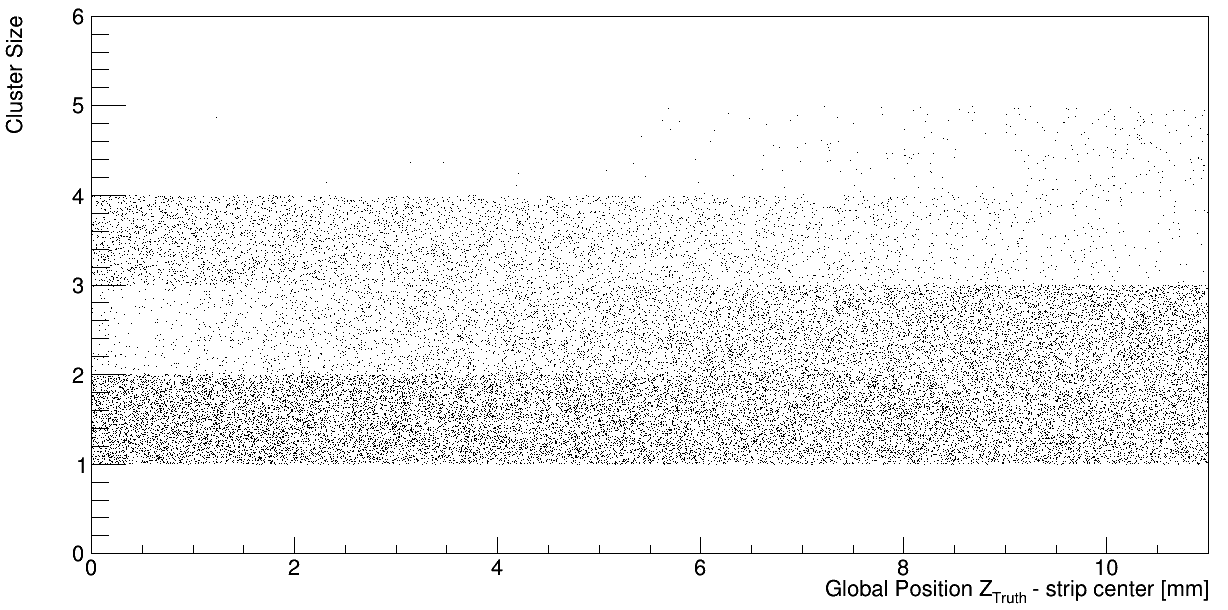
\includegraphics[width=0.83 \textwidth]{Chapters/CH3/figures/clusterSize_BI_stripCenterEta}} 
	\subfigure[] {\label{fig:strips_phi}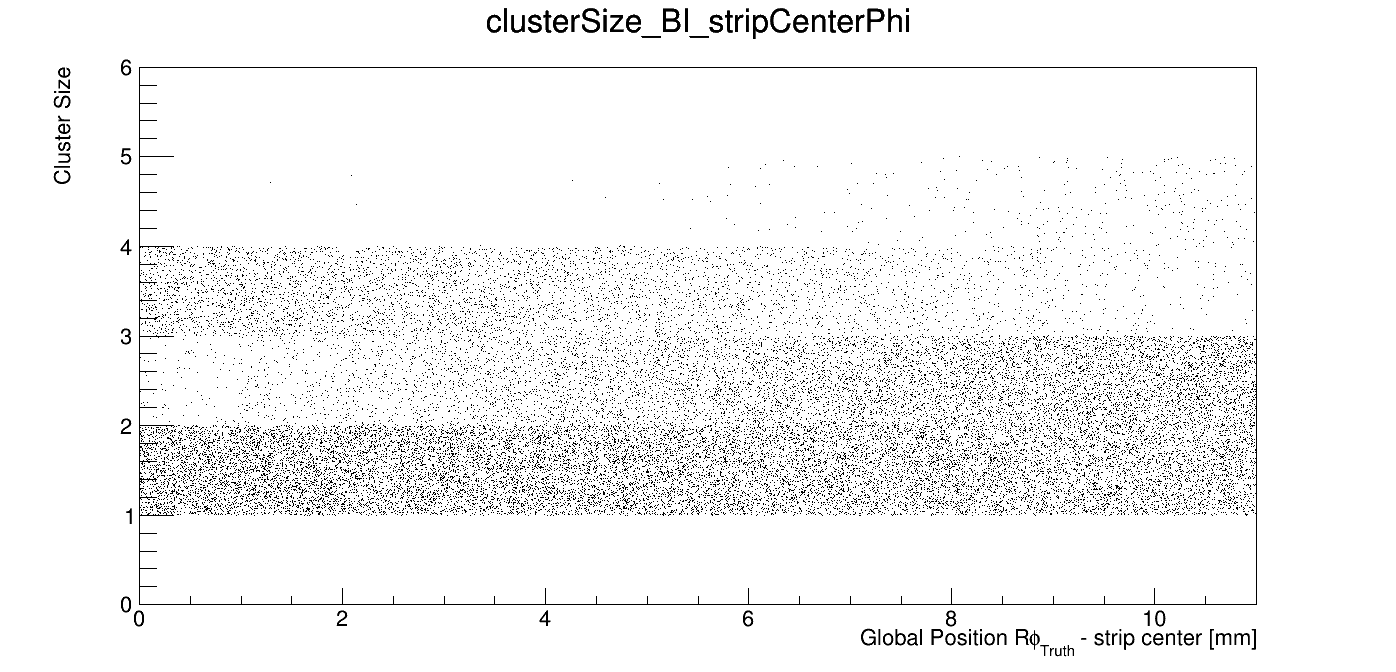
\includegraphics[width=0.83 \textwidth]{Chapters/CH3/figures/clusterSize_BI_stripCenterPhi}} 
	\caption{RPC hit distribution $\mathrm{GlobPos_{i}}$ for \subref{fig:strips_eta} strips along $\eta$ and \subref{fig:strips_phi} strips along $R\phi$.}
	\label{fig:strips}
\end{figure}	
Strips in $\eta$ and $\phi$ layers are orthogonal to each other and it is possible to see how 
they are arranged as a function of the Global Position in the BI region of the ATLAS detector.\\
In particular, in Figure ~\ref{fig:Nstrips_eta} strips oriented along $\eta$ are ordered in such a 
way that the strip number one is the inner strip, while Figure ~\ref{fig:Nstrips_phi} shows that 
strips oriented along $\phi$ are always oriented with increasing $\phi$. 
\begin{figure}[!h]
	\centering	
	\subfigure[] {\label{fig:Nstrips_eta}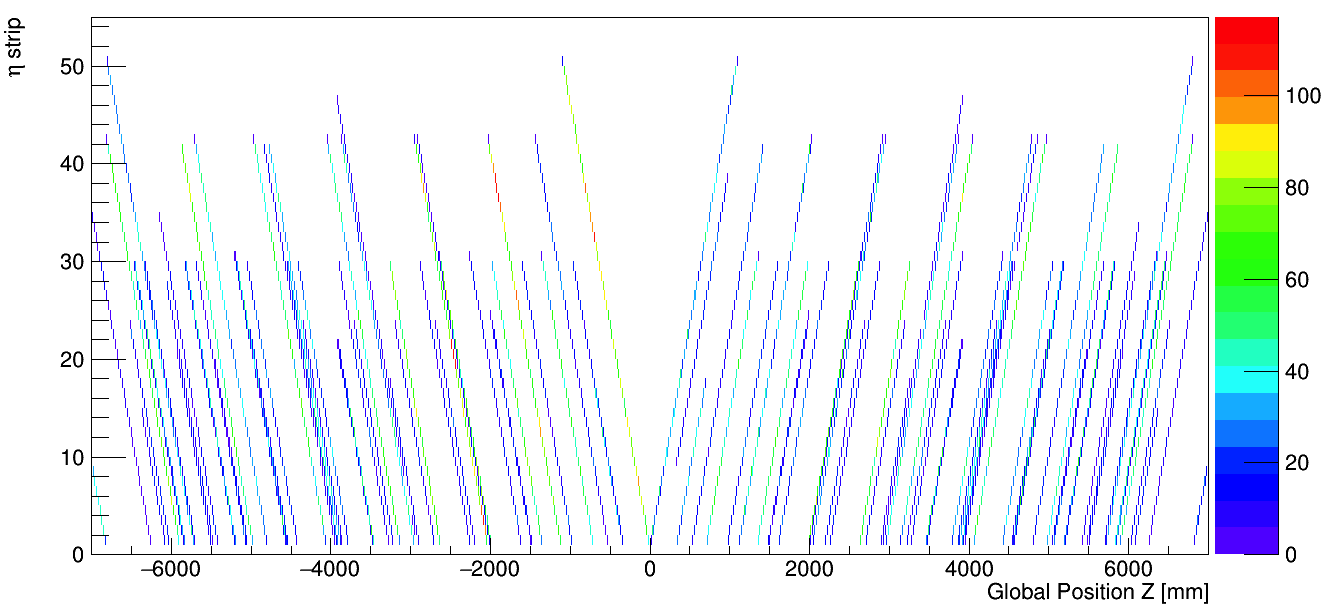
\includegraphics[width=1 \textwidth]{Chapters/CH3/figures/h_globalPos_StripEta}} 
	\subfigure[] {\label{fig:Nstrips_phi}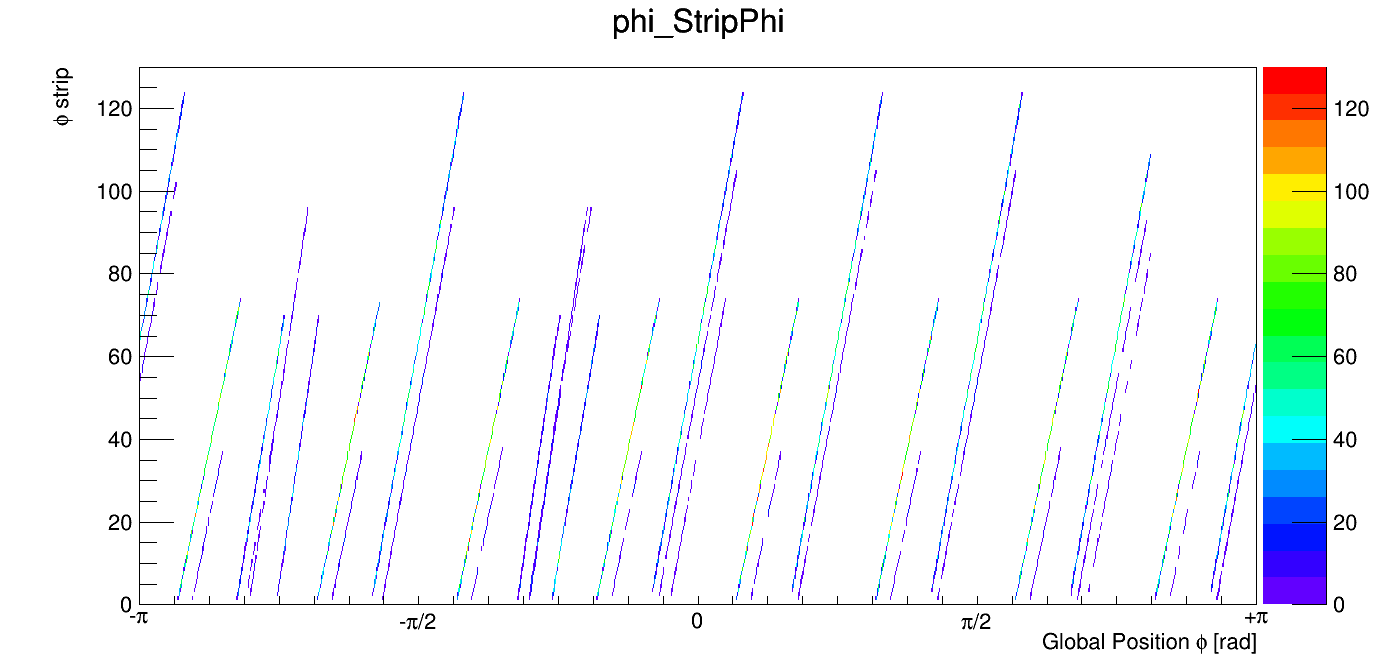
\includegraphics[width=1 \textwidth]{Chapters/CH3/figures/h_phi_StripPhi}} 
	\caption{Arrangement of strips in the \subref{fig:Nstrips_eta} $\eta$ layer and \subref{fig:Nstrips_phi} $\phi$ layer as a function of the Global Position in the BI region of the ATLAS detector.}
	\label{fig:Nstrips}
\end{figure}	
\newpage
\noindent \Cref{fig:param_BIL,fig:param_BIR} summarises the main chamber parameters of the expected layout 
for the Phase-II upgrade. Strip and front-end board 
entries are based on the assumptions of a 20 mm pitch and eight channels per board.\\
Figure~\ref{fig:strips_BI} shows the number of $\eta$ and $\phi$ strips switched on in the 
simulation. It is possible to verify that the simulation developed for this work follows the requirements of the Phase-II upgrade for BI RPCs to be realistic and reliable as much as possible.
\begin{table}[!h]
	\centering	
	\subfigure[] {\label{fig:param_BIL}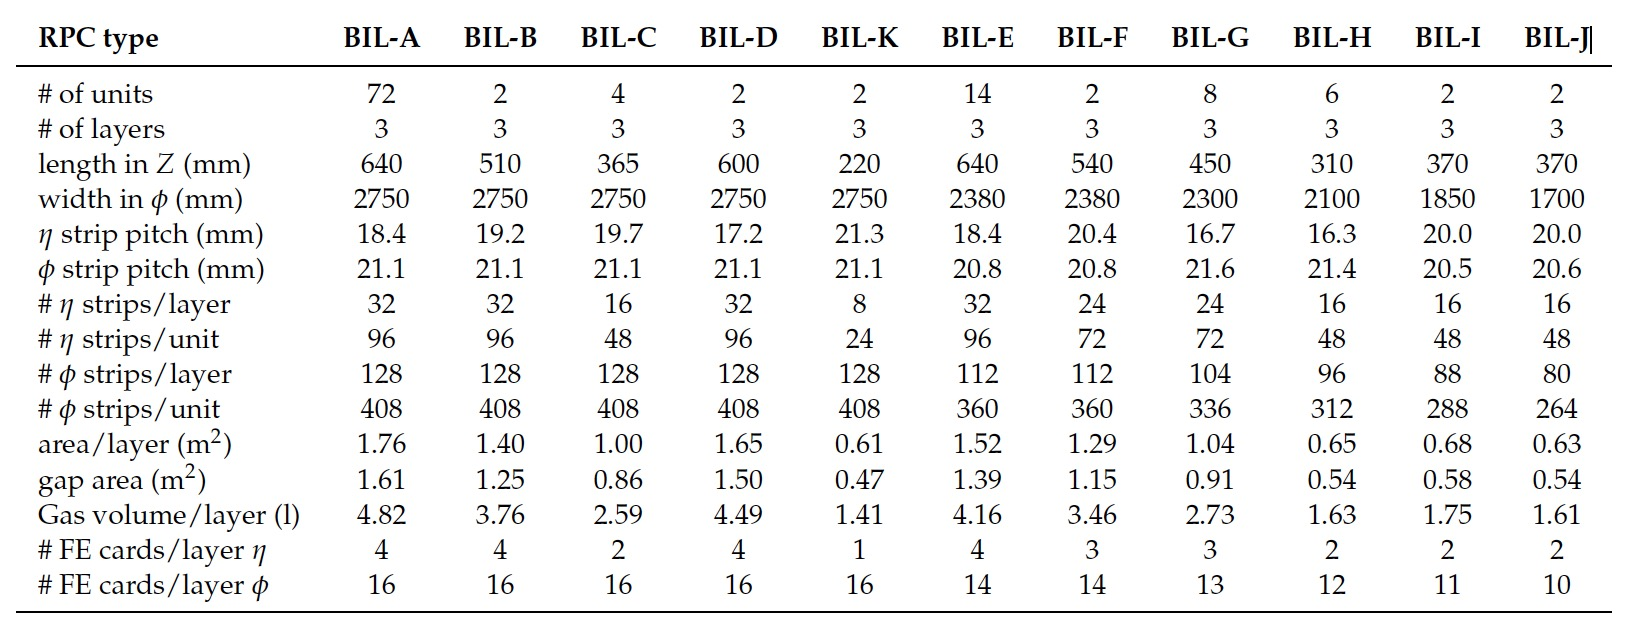
\includegraphics[width=1 \textwidth]{Chapters/CH3/figures/param_BIL}} 
	\subfigure[] {\label{fig:param_BIR}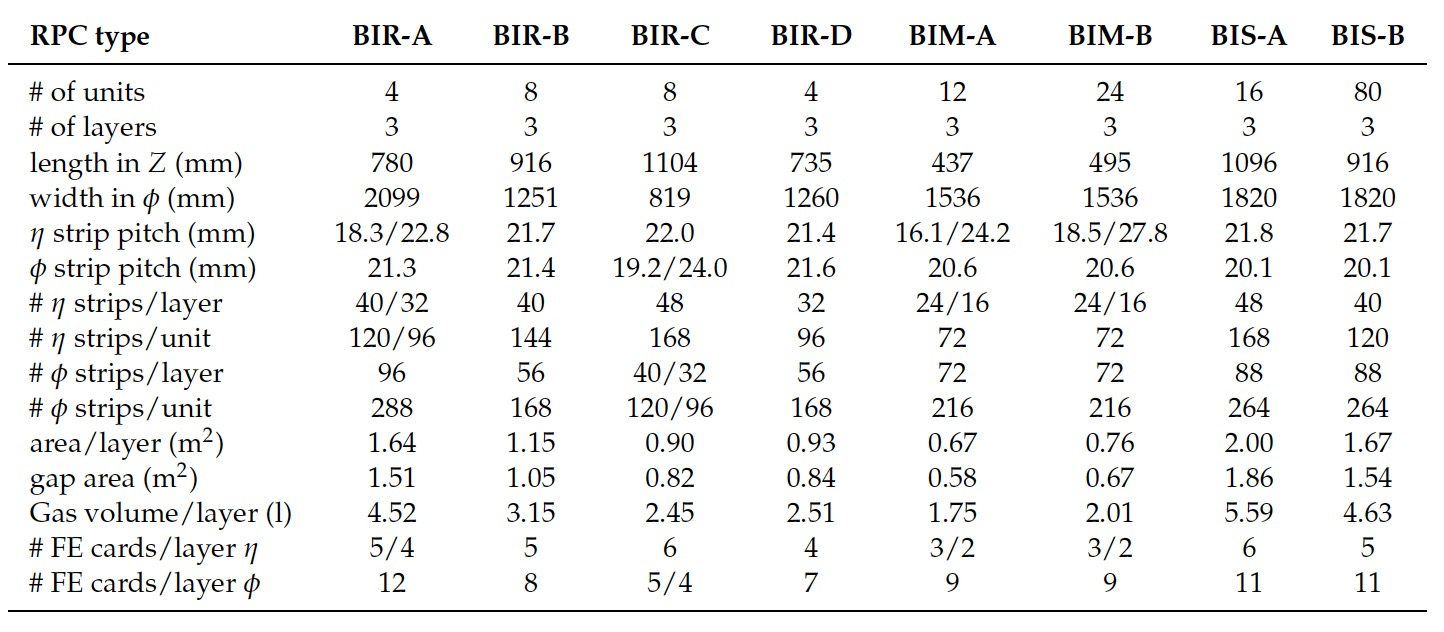
\includegraphics[width=1 \textwidth]{Chapters/CH3/figures/param_BIR}} 
	\caption{Main parameters of \subref{fig:param_BIL} the BIL RPC chambers and \subref{fig:param_BIR} the BIR/BIM/BIS RPC chambers~\cite{TDR}.}
	\label{fig:param}
\end{table}	
\begin{figure}[!h]
	\centering	
	\subfigure[] {\label{fig:CS_eta}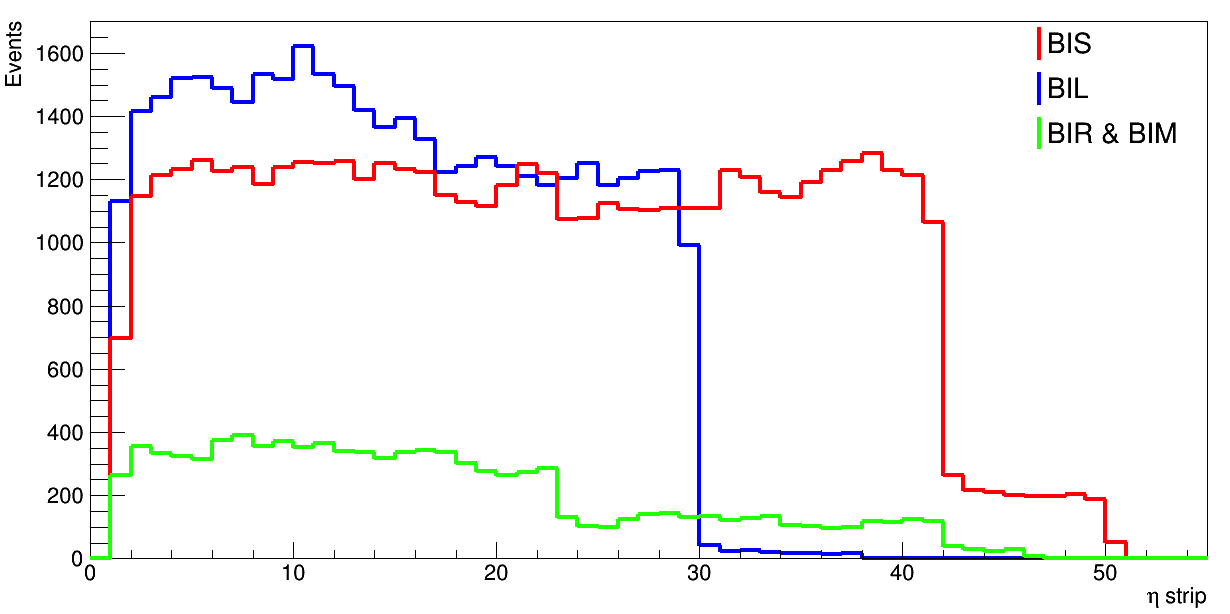
\includegraphics[width=0.95 \textwidth]{Chapters/CH3/figures/stripEta_BI}} 
	\subfigure[] {\label{fig:CS_phi}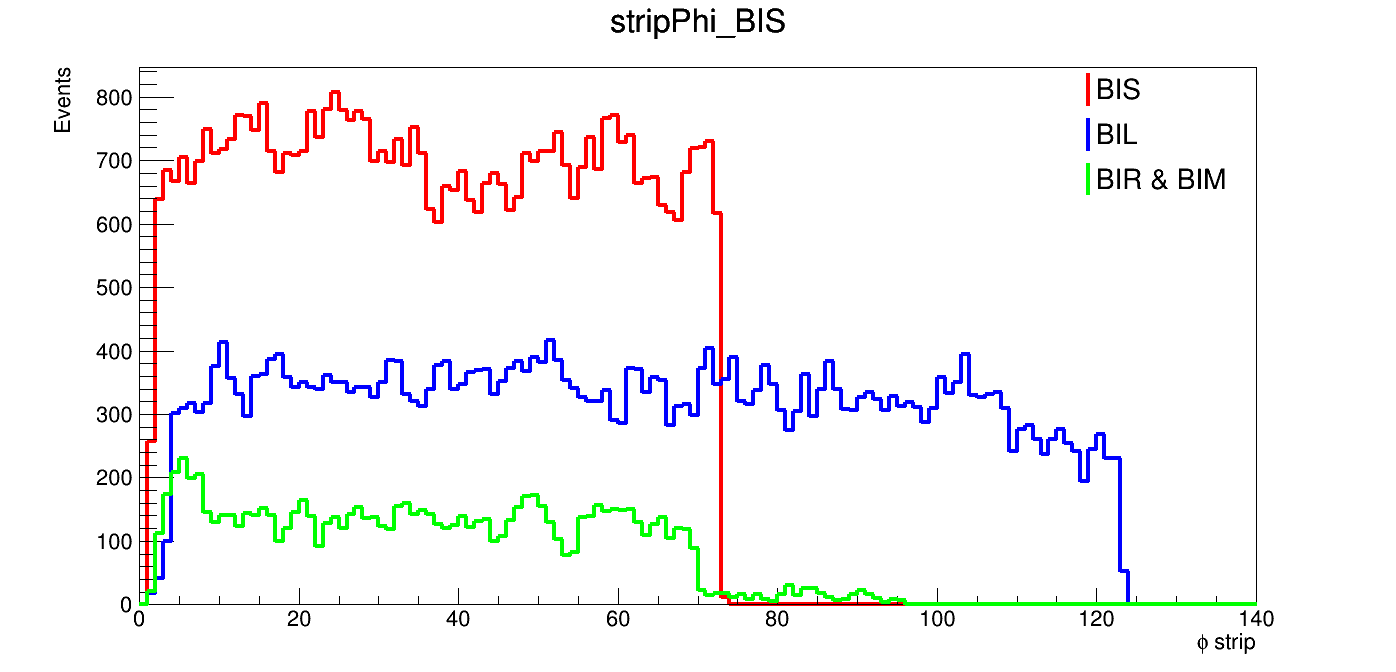
\includegraphics[width=0.95 \textwidth]{Chapters/CH3/figures/stripPhi_BI}} 
	\caption{Number of $\eta$ and $\phi$ strips switched on for different chambers:  BIS in red, BIL in blue, BIR \& BIM in green.}
	\label{fig:strips_BI}
\end{figure}	
\FloatBarrier

\subsection{Timing}
\label{sec:timing}
Another important variable is the time taken for the particle to pass through the detector. It is 
important because it is one of the discriminating variables in the algorithm's selection of hits. 
Only hits recorded in the bunch crossing event are considered and not all the hits previously recorded. 
Therefore, all hits outside 25~ns coincidence window around the bunch crossing of interest are 
excluded.\\
In order to simulate the new RPCs one has to take into account several effects and apply an 
appropriate correction and extract a digital readout.
\vspace{\baselineskip}\\
The final formula used to extract the digitized time in which the hit is recorded by the detector is:
\begin{equation}
t_{hit}= int\footnotemark\bigg\{\frac{t_{true}+t_{Gauss}+t_{FE}-t_{cal}}{\Delta t}\bigg\}\Delta t
\label{eq:timing}
\end{equation}
\begin{itemize}
	\item $t_{true}$ is the true hit recorded by the MDT;
	\item $\Delta t$ is the sampling rate (0.3 ns). The final $t_{hit}$ must be a multiple of the sampling rate to have a digitization;
	\item $t_{Gauss}$ is a Gaussian term that reproduces the fluctuations in the RPC signal 
	(smearing 0.4 ns);
	\item $t_{FE}$ is the propagation of the signal along the strip to the FE electronics 
	assuming  that the signal speed on the layer is 200 mm/ns;
	\item $t_{cal}$ is the calibration offset. The true hit timing is recorded referring to the time 
	of the collision on the MDT tubes. To report the timing centered around 0, it was necessary to 
	subtract the time of flight of the particle assuming time to be calibrated with 
	prompt muons crossing the center of the strip at t = 0.
\vspace{\baselineskip}\\	
Figure~\ref{fig:time_BI} shows the digitized time associated to the RPC hit calculated using the 
Equation~\ref{eq:timing}. The tail of the distribution is given by low $p_T$ muons  that produce 
secondary hits.
\end{itemize} 

\begin{figure}[!h]
	\centering
	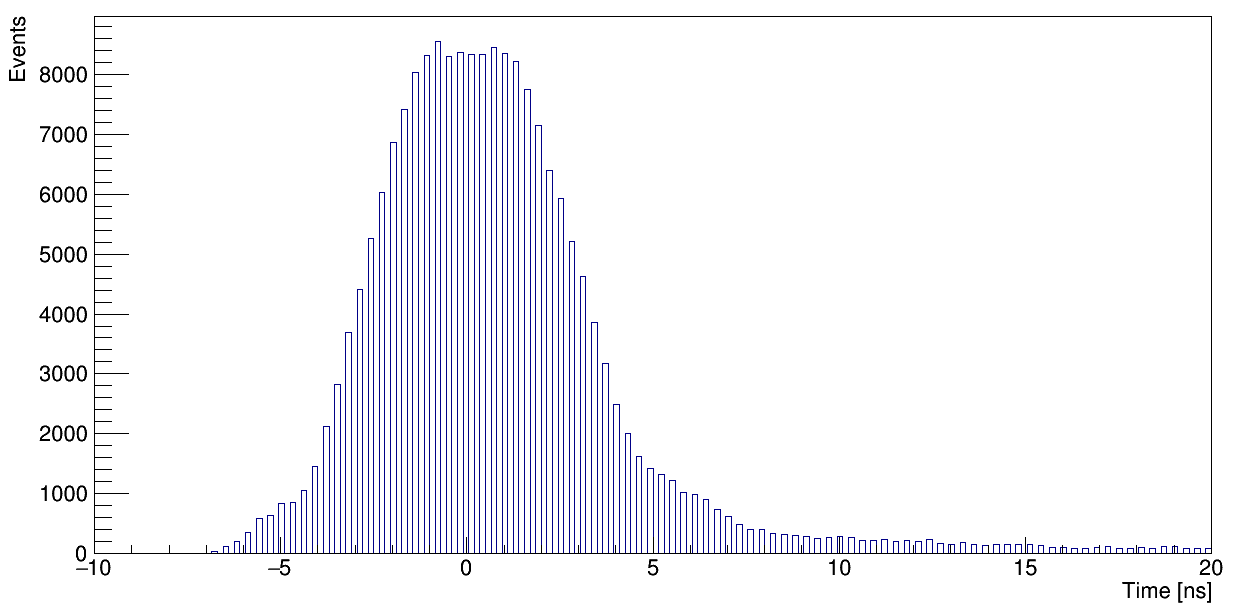
\includegraphics[width=0.9\textwidth]{Chapters/CH3/figures/time_BI}
	\caption{Digitized time associated to the RPC hit. The tail of the distribution is given by low 
		$p_T$ muons that produce secondary hits}
	\label{fig:time_BI}
\end{figure}

\footnotetext{The $int$ function takes the integer part of a real number.}

\section{L0 barrel trigger efficiency}
\label{sec:eff}
The performance of the barrel muon trigger was studied using single-muon MC samples with fixed \pT = 50 \GeV, for a fixed transverse momentum threshold: $p_{T} > 10$ GeV~\cite{Marcoccia:2693982} and with the hit digitization described in the previous sections.\\
To study the robustness of the trigger against possible efficiency reductions of the old RPCs in the BM and BO layers, the simulation was performed in the so-called "worst-case scenario" that introduces inefficiencies depending on the station type and sector and summarised as Table~\ref{tab:WCS}. It includes inefficiencies due to a reduction of the high voltage of the BM and BO RPCs such that the expected RPC current is always below the safe operation limit.
\begin{table}[htbp]
	\begin{center}
		\begin{tabular}{c|cccccccc}
			\multirow{2}{*}{\textbf{Station Name}} & \multicolumn{8}{c}{\textbf{StationEta}}\\
			\cline{2-9}
			& \textbf{1} & \textbf{2} & \textbf{3} & \textbf{4} & \textbf{5} & \textbf{6} & \textbf{7} & \textbf{8}\\
			\hline 
			BOL                 				   & 0.90  	    & 0.90		 & 0.82 	  & 0.82 	   & 0.76 		& 0.74 		 & -	      & -    \\
			BOS/BOG/BOF 						   & 0.89 		& 0.90 		 & 0.90 	  & 0.90	   & 0.89 		& 0.66 		 & 0.60       & 0.60 \\
			BML                					   & 0.88		& 0.88 		 & 0.88 	  & 0.83 	   & 0.56 		& 0.56		 & 0.60       & -    \\
			BMS              					   & 0.90  	    & 0.90		 & 0.90 	  & 0.87 	   & 0.81 	    & 0.81    	 & -          & -    \\
			\hline 
		\end{tabular} 
		\caption{Efficiency for each station and sector of the barrel muon trigger in the "worst-case scenario". This scenario includes inefficiencies due to a reduction of the HV of the BM and BO RPC~\cite{Marcoccia:2693982}.} 
		\label{tab:WCS}
	\end{center} 
\end{table} 
\noindent The trigger efficiency times acceptance for each trigger logic scheme is listed in Table~\ref{tab:eff_x_acc_wcs} and it is defined as the fraction of reconstructed muons that are accepted by the trigger, using the simulation that includes the RPC detector efficiency.
The trigger efficiency times acceptance is also presented in Figure~\ref{fig:h_eff}. 
Adding the new BI RPC layer greatly reduces the dependence of the trigger efficiency on the hit efficiency of the old RPCs.
\begin{table}[h]
		\small
\begin{tabular}{l|c|c|c}
	\hline
	\multirow{2}{*}{\textbf{BM and BO efficiency (\%)}} & \multicolumn{3}{c}{\textbf{Trigger efficiency x acceptance (\%)}}\\
	\cline{2-4}   
	& \textbf{3/3 chambers} & \textbf{3/4 chambers} & \textbf{3/4 chambers + BIBO}\\
	\hline 
	WCS 												& 58.78 				& 83.27 		& 91.89\\
	\hline 
\end{tabular} 
\caption{Efficiency times acceptance for the L0 barrel trigger for each trigger logic scheme, assuming the worst-case scenario with the hit digitization  .} 
\label{tab:eff_x_acc_wcs}
\end{table} 
\begin{figure}[!h]
	\centering
	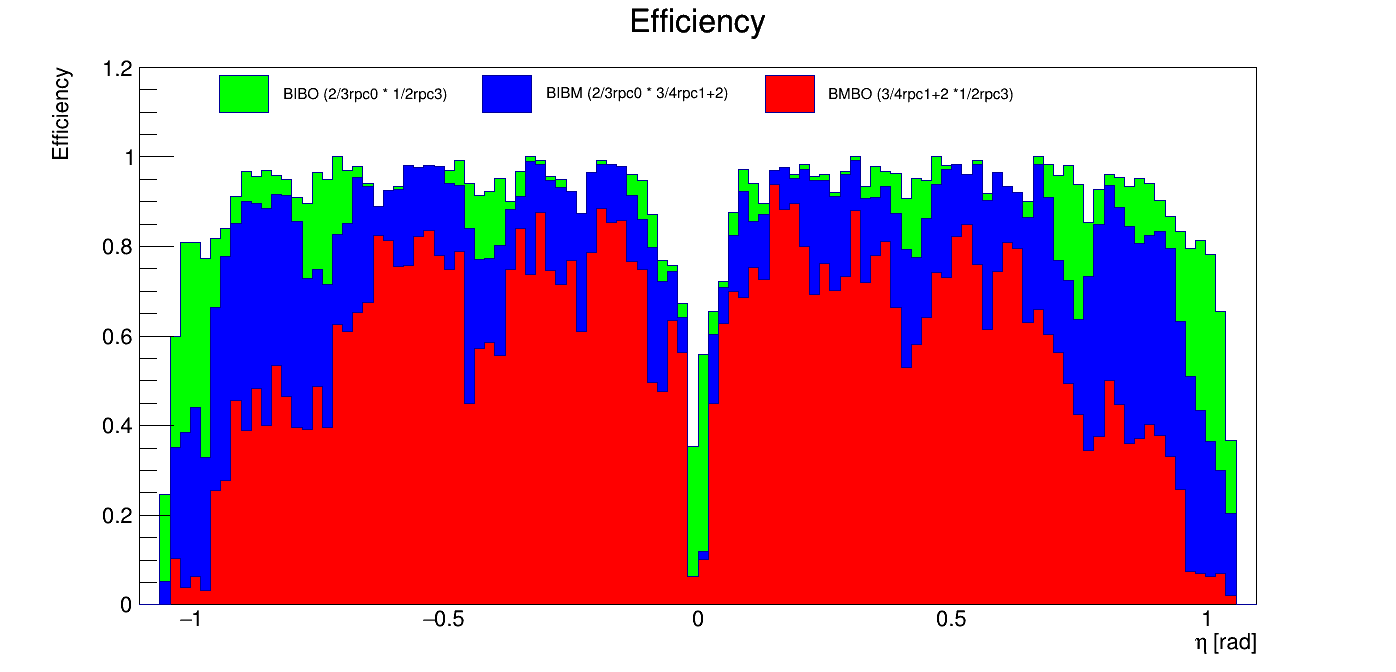
\includegraphics[width=1.1\textwidth]{Chapters/CH3/figures/h_eff}
	\caption{Efficiency times acceptance of the L0 barrel trigger for each trigger logic scheme, assuming the worst-case scenario with the hit digitization.}
	\label{fig:h_eff}
\end{figure}
\\Starting from the WCS scenario, other two studies have been performed on the L0 barrel trigger 
efficiency using simulations with RPC stations in various operational conditions: the first study is the  refurbish of BM and BO chambers (Section~\ref{sec:BMBO_retrofit}) and the second study is about the installation of BI chambers in the rail sectors 11 and 15 (Section~\ref{sec:BIRBIM_drop}).

\subsection{BM and BO retrofitting}
\label{sec:BMBO_retrofit}
In the Phase-II upgrade of the muon system, most of the readout electronics will
be replaced to make it faster and resistant to radiation.
An essential step is therefore to understand what would be the impact of the legacy BM/BO chambers with the new electronics.\\
In this first study, efficiencies of the "worst-case scenario" summarised in Table~\ref{tab:WCS}, are used, except for the following stations set to 100\% efficiency:
\renewcommand{\labelenumii}{\Lowercase{enumii}}
\begin{enumerate}
\item BML 7,
\item BOL 6,
\item BOS 6,
\item BOL 5.
\end{enumerate}
The products of muon trigger efficiency and acceptance for the BM and BO retrofitting are listed in Table~\ref{tab:allcasesBMBO}.\\
The trigger efficiency times acceptance is also presented in Figure~\ref{fig:allcasesBMBO} that compare the "worst-case scenario" with all the variants of the WCS, in which some stations are fixed to 100\% efficiency.\\
In the first analysed case, the most relevant effect on the trigger efficiency times acceptance is on the 3/4 chambers logic scheme, in particular for the Case 1b (BOL 6 100\%) the variation is +1.08\% compared to the "worst-case scenario".
\begin{table}[h]
	\begin{center}
		\small
		\begin{tabular}{l|c|c|c}
			\hline
			\multirow{2}{*}{\textbf{BM and BO efficiency (\%)}} & \multicolumn{3}{c}{\textbf{Trigger efficiency x acceptance (\%)}}\\
			\cline{2-4}   
			& \textbf{3/3 chambers} & \textbf{3/4 chambers} & \textbf{3/4 chambers + BIBO}\\
			\hline 
			WCS 												& 58.78 				& 83.27 		& 91.89\\
			Case 1a (BML 7 100\%) 								& +0.22                 & +0.26 		& +0.14\\
			Case 1b (BOL 6 100\%) 								& +0.13 				& +1.08 		& +0.53\\
			Case 1c (BOS 6 100\%) 								& +0.16 				& +0.51 		& +0.63\\
			Case 1d (BOL 5 100\%) 								& +0.23 				& +0.82 		& +0.41\\		
			\hline 
		\end{tabular} 
		\caption{Efficiency times acceptance for the L0 barrel trigger for different assumptions on the hit efficiency of the present RPC detectors. The “WCS” row corresponds to the scenario in which the efficiencies are listed in Table~\ref{tab:WCS}. The other rows correspond to the variants of the WCS, in which the efficiency of some stations are set to 100\%. The corresponding results of these variants, are expressed as variations to the WCS~\cite{Marcoccia:2693982}.} 
		\label{tab:allcasesBMBO}
	\end{center} 
\end{table} 

\begin{figure}[h]
	\centering
	\subfigure [3/3 chamber]{{\label{fig:allcasesBMBO_a}}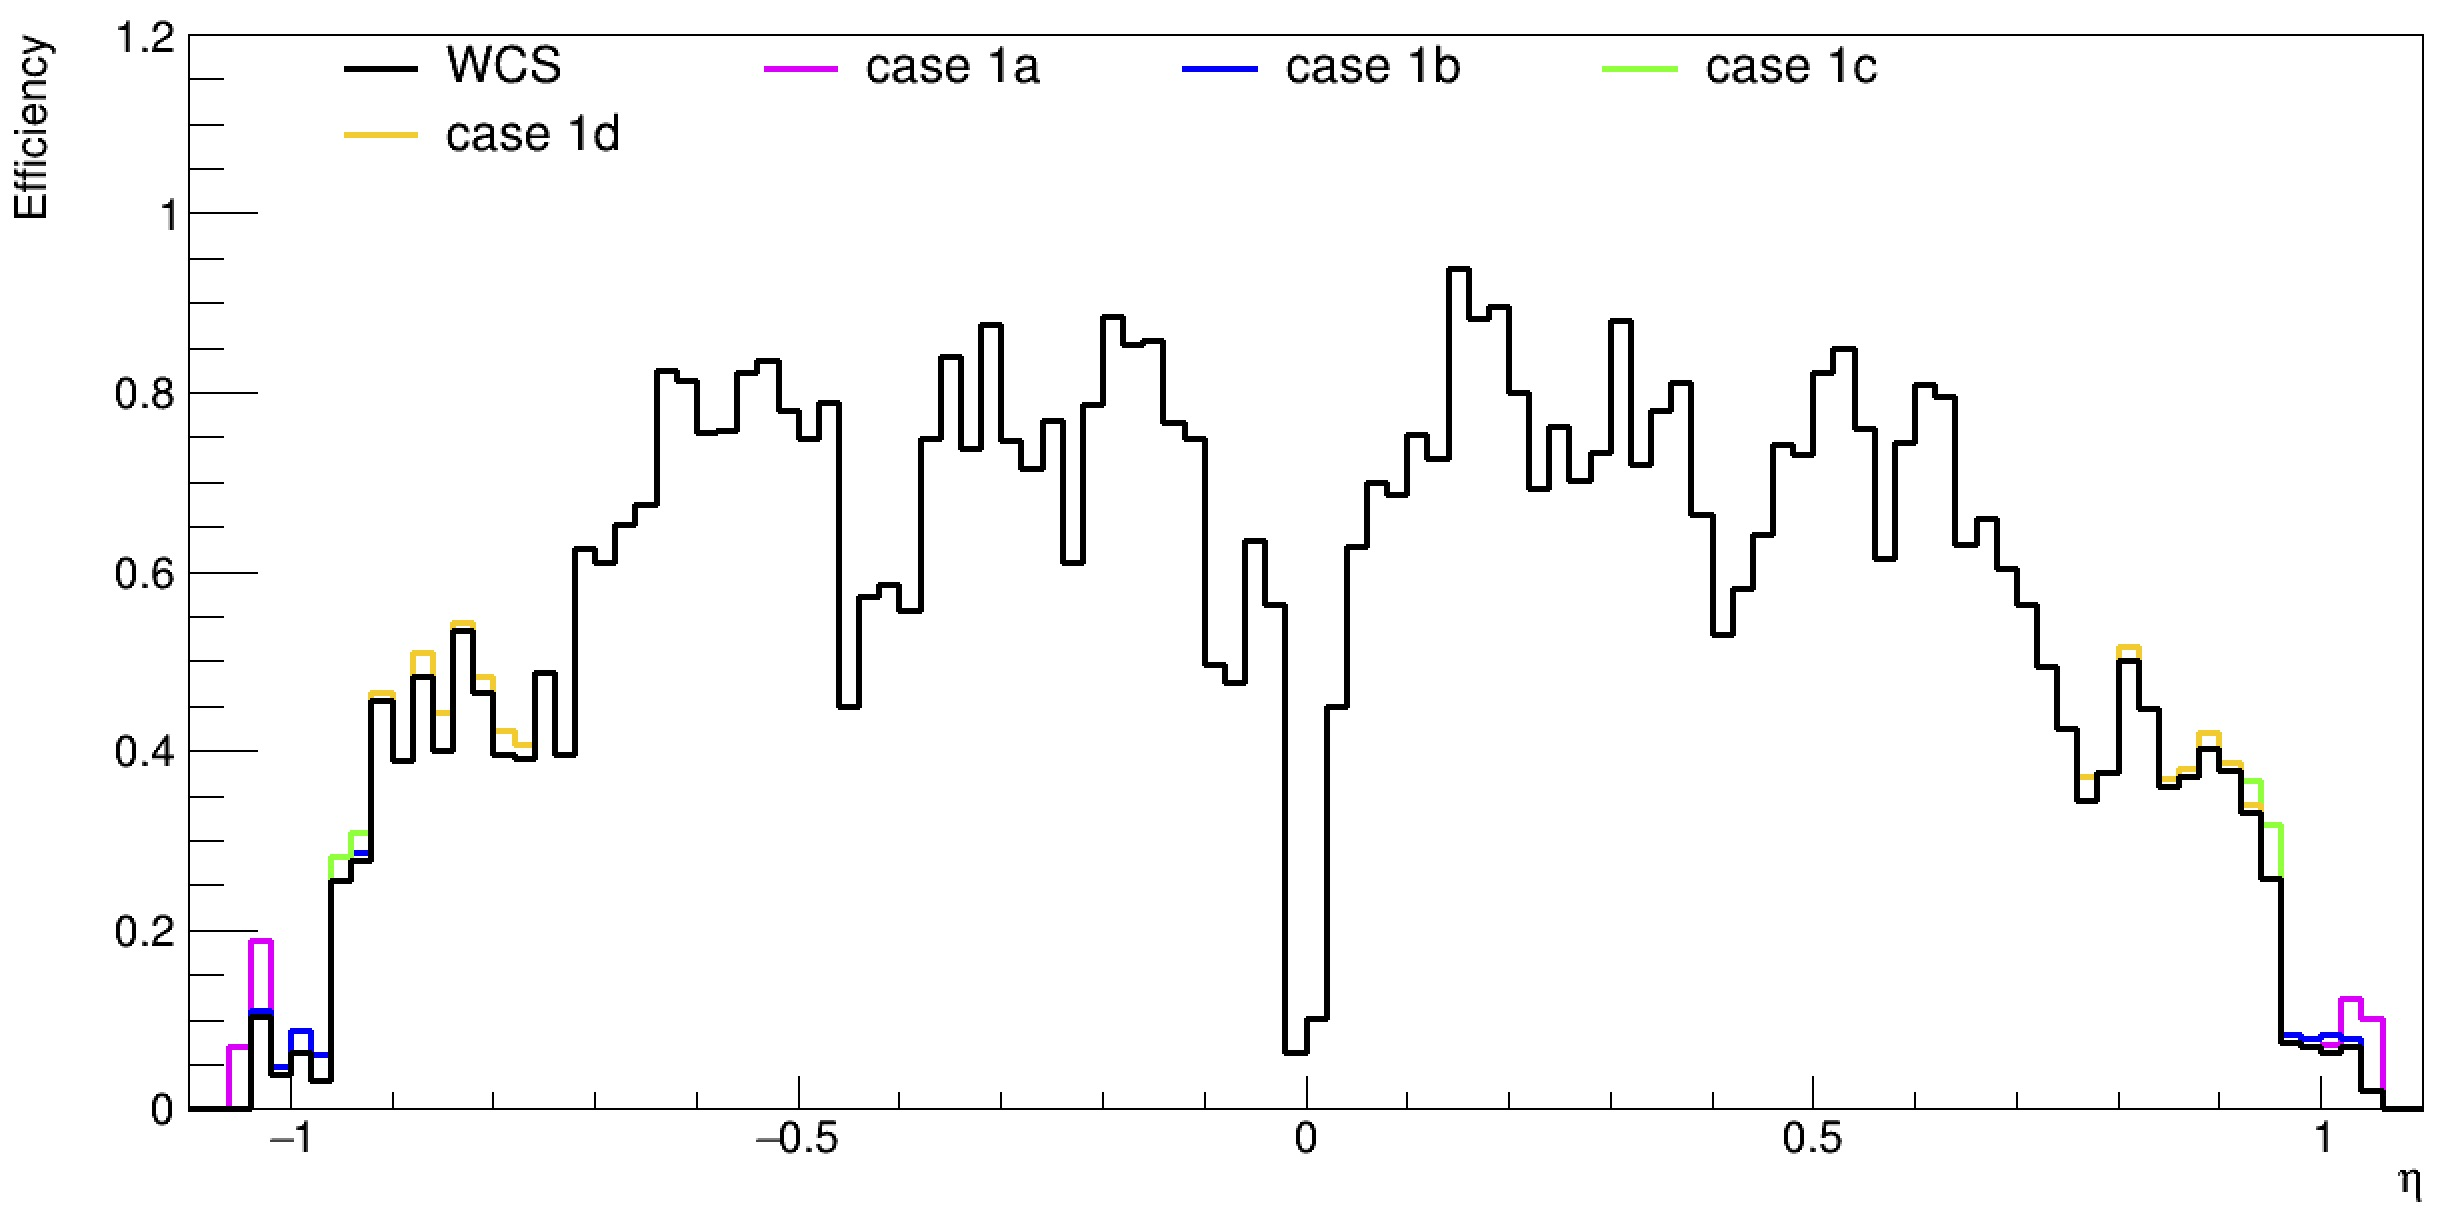
\includegraphics[width=0.95 \textwidth]{Chapters/CH3/figures/BMBO_firstCase}} 
\end{figure}	
\begin{figure}[h]
	\centering
	\subfigure [3/4 chambers]{{\label{fig:allcasesBMBO_b}}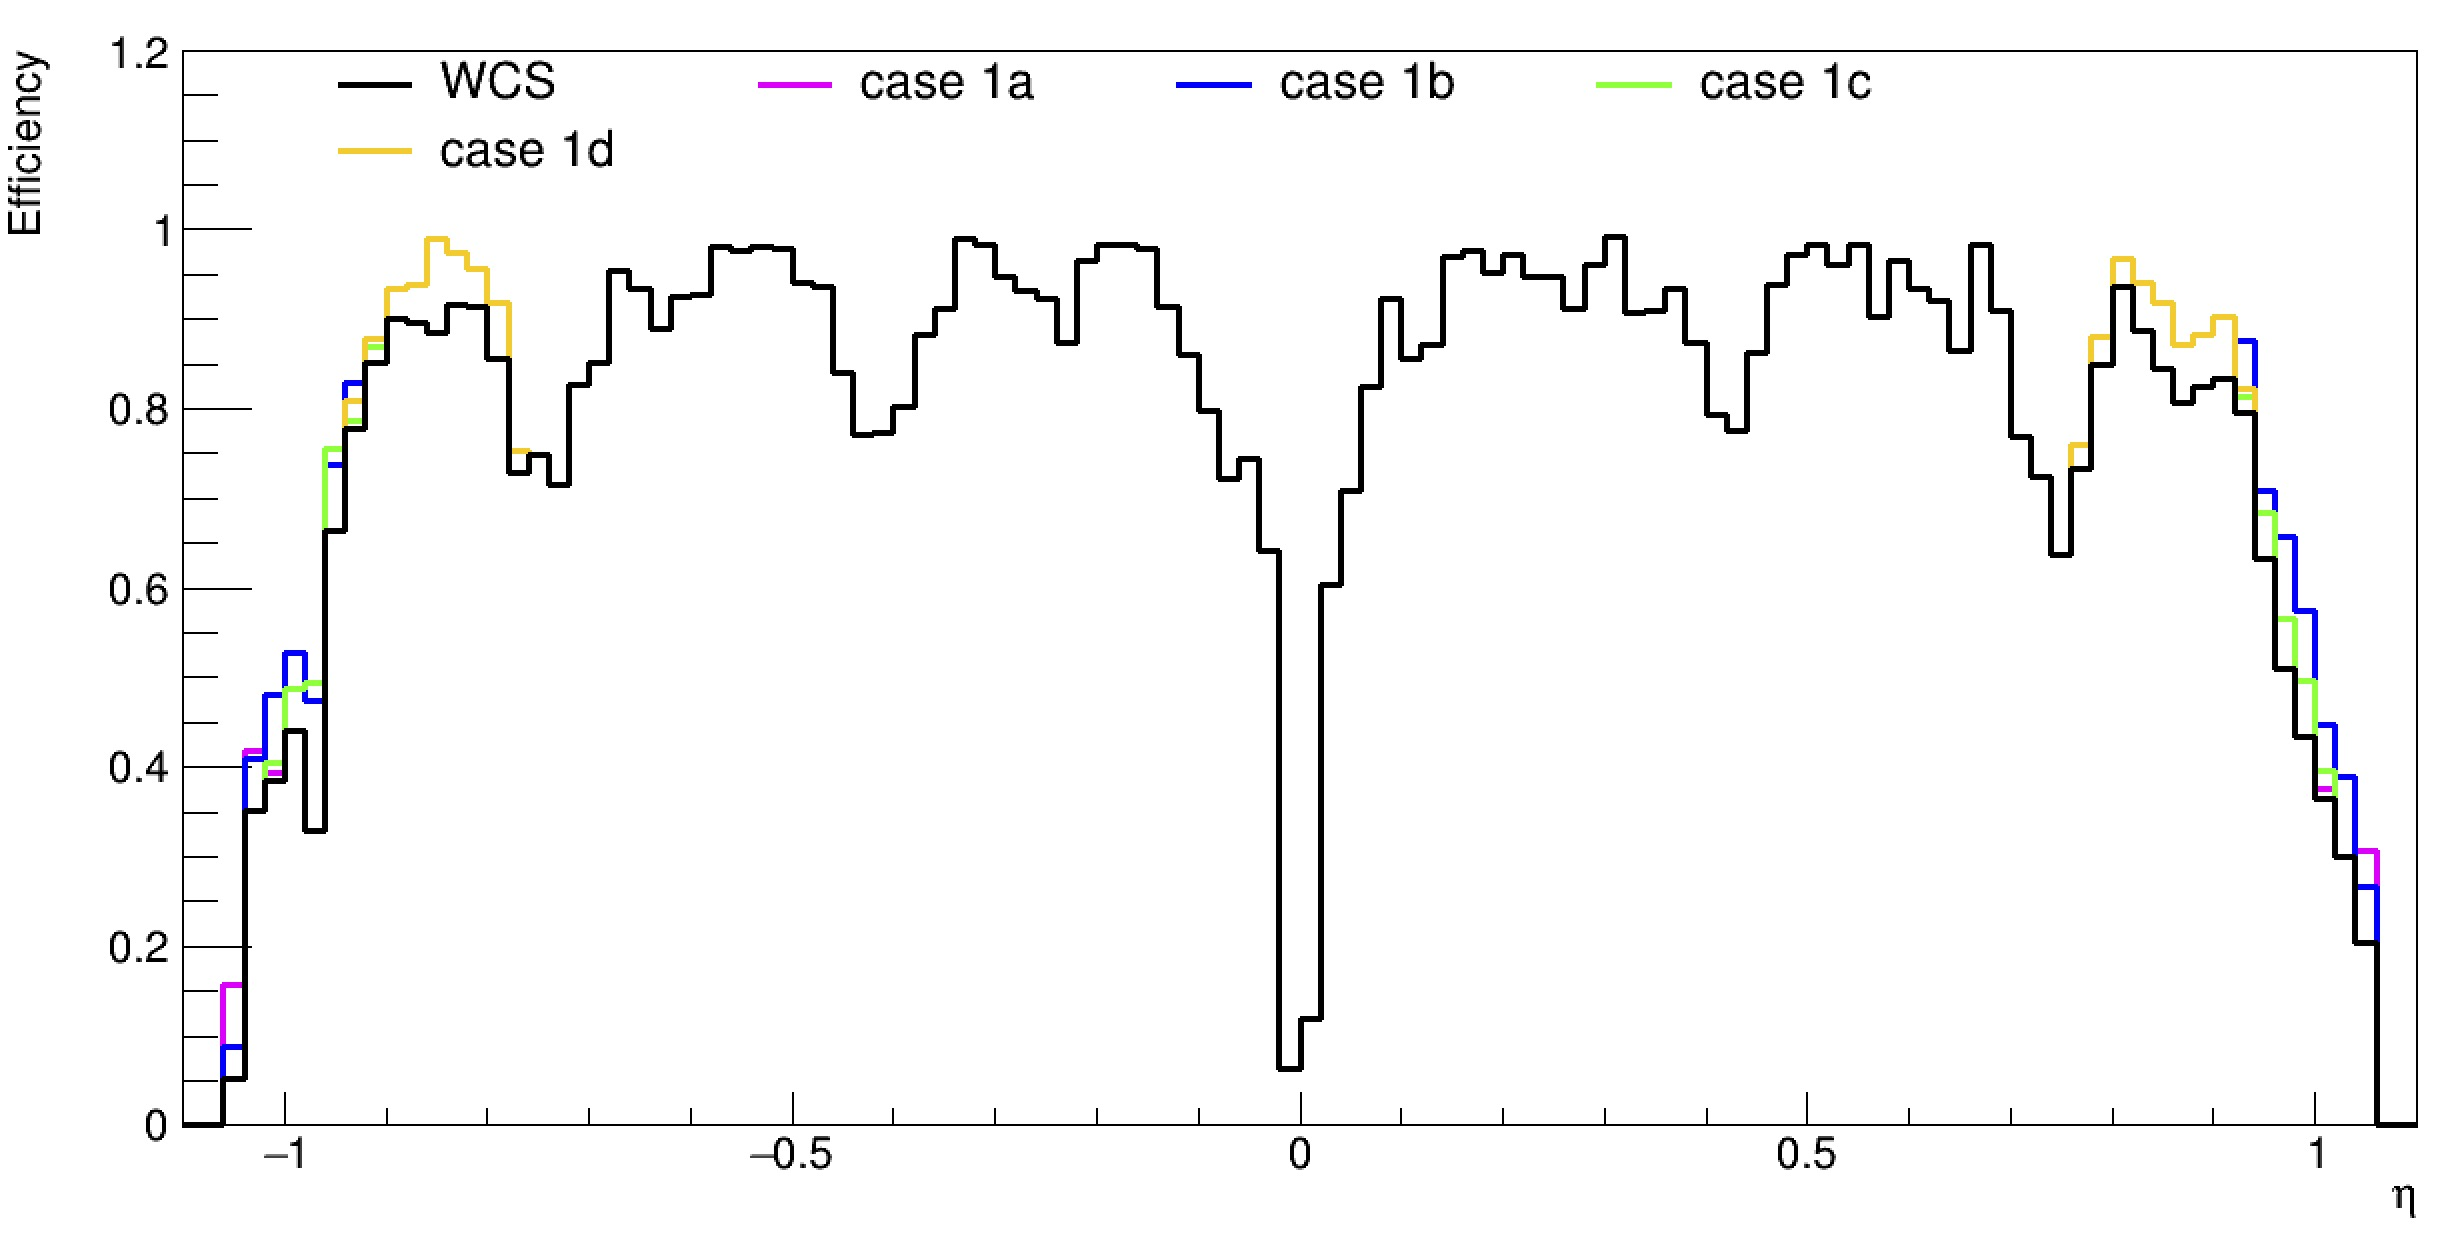
\includegraphics[width=0.95 \textwidth]{Chapters/CH3/figures/BIBM_firstCase}} 
	\subfigure [3/4 chambers + BIBO]{{\label{fig:allcasesBMBO_c}}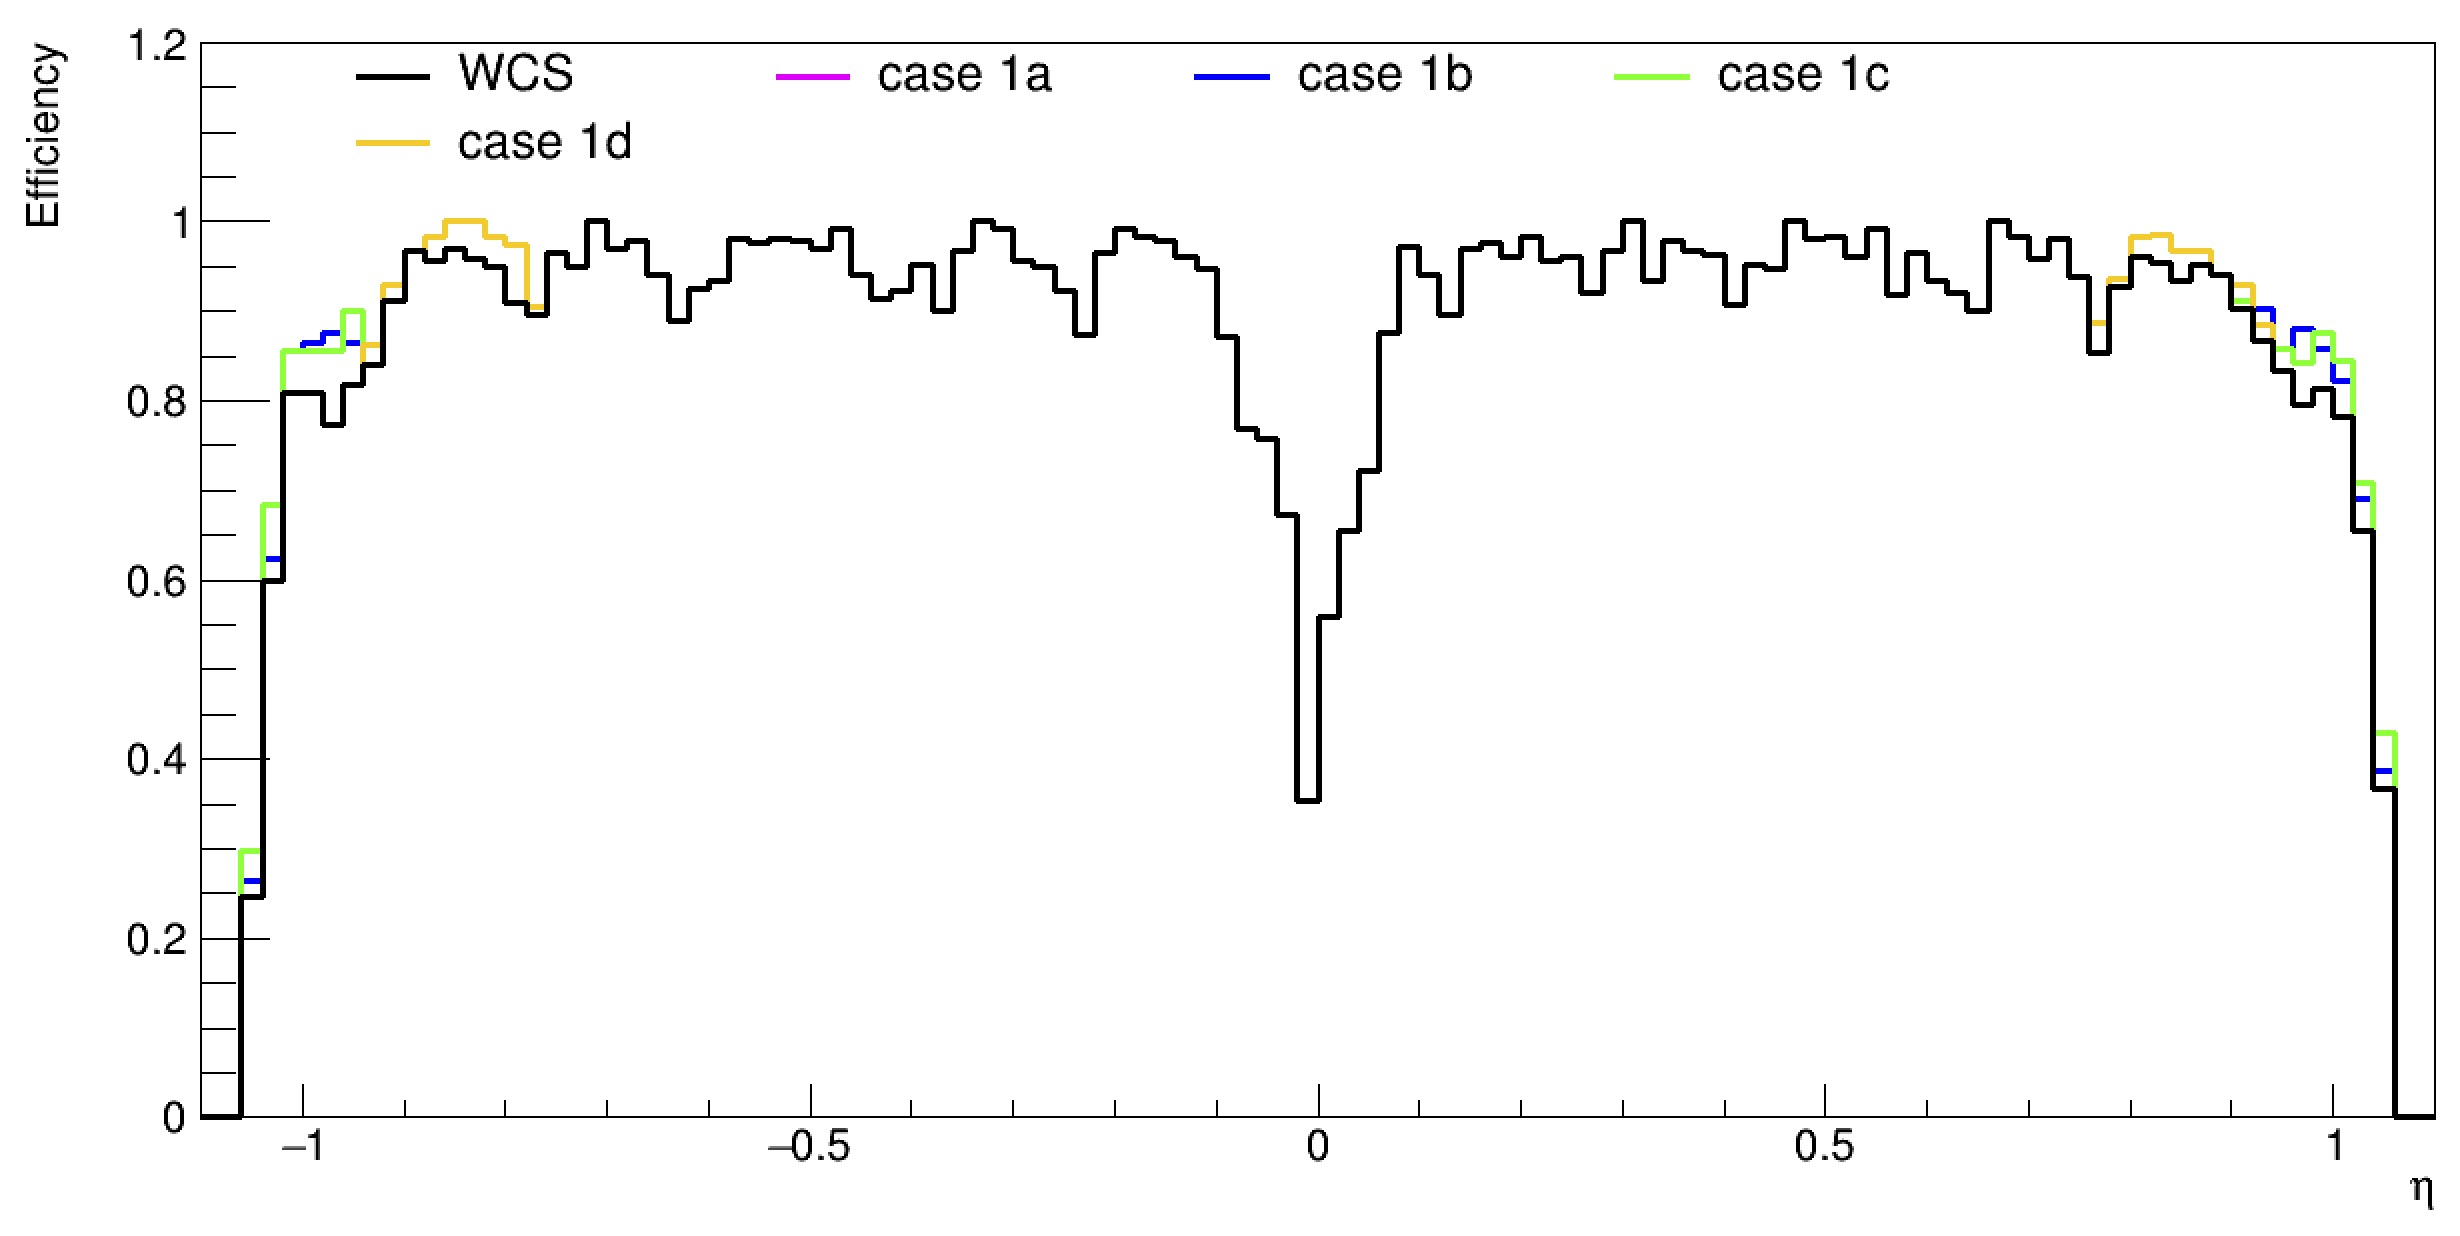
\includegraphics[width=0.95 \textwidth]{Chapters/CH3/figures/BIBO_firstCase}} 
	\caption{Efficiency times acceptance of the L0 barrel trigger compared to reconstructed muons with $p_{T} = 50$ GeV as a function of $\eta$ taking in to account all the variants of the WCS. The histograms show the efficiency of \subref{fig:allcasesBMBO_a} the existing 3/3 chambers trigger, of \subref{fig:allcasesBMBO_b}  the 3/4 chambers trigger including the BI layer, and \subref{fig:allcasesBMBO_c}  the additional gain from the BI-BO trigger. Efficiency times acceptance is defined as the fraction of reconstructed muons accepted by the trigger, using a simulation that includes the RPC detector efficiency~\cite{Marcoccia:2693982}.}
	\label{fig:allcasesBMBO}
\end{figure}

\FloatBarrier
\subsection{Dropping BIR and BIM chambers}
\label{sec:BIRBIM_drop}
Since the installation of the RPCs in the sectors 11 and 15  seems to be very hard, another special case was performed simulating a scenario in which BIM and BIR RPC are not installed in these sectors.\\
The products of muon trigger efficiency and acceptance for this second study are listed in Table~\ref{tab:allcasesBIRBIM}.\\
The results are also presented in Figure~\ref{fig:allcasesBIRBIM} that compares the "worst-case scenario" with this second case, in which BIM and BIR are turned off.
The efficiency distributions show that the absence of BIR and BIM has the most relevant effect on the 3/4 chambers + BIBO logic scheme with a corresponding variation of -3.11\%.

\begin{table}[h]
	\begin{center}
		\small
		\begin{tabular}{l|c|c|c}
			\hline
			\multirow{2}{*}{\textbf{BM and BO efficiency (\%)}} & \multicolumn{3}{c}{\textbf{Trigger efficiency x acceptance (\%)}}\\
			\cline{2-4}   
			& \textbf{3/3 chambers} & \textbf{3/4 chambers} & \textbf{3/4 chambers + BIBO}\\
			\hline 
			WCS 												& 58.78 				& 83.27 				& 91.89\\
			Case 2  (BIM BIR off)								& +0.03 			   	& -2.70 				& -3.11\\
			\hline 
		\end{tabular} 
		\caption{Efficiency times acceptance for the L0 barrel trigger for different assumptions on the hit efficiency of the present RPC detectors. The WCS row corresponds to the scenario in which the efficiencies are listed in Table~\ref{tab:WCS}. The row "Case 2" corresponds to the case in which the RPCs in the sectors 11-15 (BIM and BIR) are turned off. The corresponding results of the Case 2, are expressed as variations to the WCS~\cite{Marcoccia:2693982}.} 
		\label{tab:allcasesBIRBIM}
	\end{center} 
\end{table} 
%\subfloat [Case 1a: BML 7 100\%] {\includegraphics[width=.5 \textwidth]{figures/h_eff_1a}} 
%\subfloat [Case 1b: BOL 6 100\%] {\includegraphics[width=.5 \textwidth]{figures/h_eff_1b}} \\
%\subfloat [Case 1c: BOS 6 100\%] {\includegraphics[width=.5 \textwidth]{figures/h_eff_1c}} 
%\subfloat [Case 1d: BOL 5 100\%] {\includegraphics[width=.5 \textwidth]{figures/h_eff_1d}} \\
%\subfloat [Case  2: BIM BIR off]    {\includegraphics[width=.5 \textwidth]{figures/h_eff_2}}  

\begin{figure}[h]
	\centering
	\subfigure [3/3 chambers]{\label{fig:allcasesBIRBIM_a}\includegraphics[width=0.95 \textwidth]{Chapters/CH3/figures/BMBO_secondCase_phi}} 
\end{figure}	

\begin{figure}[h]
	\centering	
	\subfigure [3/4 chambers]{\label{fig:allcasesBIRBIM_b}\includegraphics[width=0.95 \textwidth]{Chapters/CH3/figures/BIBM_secondCase_phi}} 
	\subfigure [3/4 chambers + BIBO]{\label{fig:allcasesBIRBIM_c}\includegraphics[width=0.95 \textwidth]{Chapters/CH3/figures/BIBO_secondCase_phi}} 
	\caption{Efficiency times acceptance of the L0 barrel trigger compared to reconstructed muons with $p_{T} = 50$ GeV as a function of $\phi$. The histograms show the efficiency of \subref{fig:allcasesBIRBIM_a}  the existing 3/3 chambers trigger, of \subref{fig:allcasesBIRBIM_b} the 3/4 chambers trigger including the BI layer, and \subref{fig:allcasesBIRBIM_c} the additional gain from the BI-BO trigger. Efficiency times acceptance is defined as the fraction of reconstructed muons accepted by the trigger, using a simulation that includes the RPC detector efficiency~\cite{Marcoccia:2693982}.}
	\label{fig:allcasesBIRBIM}
\end{figure}	
\FloatBarrier

\section{Summary and considerations }
\label{sec:concl_QT}
The works described in this chapter aimed at a new simulation of the RPC in the BI region.
They involved the construction of a model:
\begin{itemize}
\item for the definition of the cluster size, which is important for creating a simulation as realistic as possible;
\item to define a variable that represents the time taken by the particle to pass through the detector, which is important because it is one of the discriminating variables in the algorithm's selection of hits.
\end{itemize}
The new developed model results in agreement with the required technical characteristics of the RPCs for Phase-II, described in the Technical Design Report~\cite {TDR}.\\
A more realistic simulation of the RPCs is now available for further studies.
\vspace{\baselineskip}
\\Using this model, L0 barrel trigger efficiency studies were performed in the following two scenarios:
\begin{enumerate}
\item the refurbish of BM and BO chambers, to understand what would be the impact of the legacy BM / BO chambers with the new electronics;
\item the drop of BIR and BIM chambers, given that the installation of the RPCs in the sectors 11 and 15 seems to be very hard.
\end{enumerate}
The first scenario gives an estimation of the improvements by replacing the electronics. Moreover, the most significant expected improvement is from BOL6.\\
The second scenario showed that there is a significant loss of efficiency if the collaboration decides to don't install the RPC in sectors 11 and 15.\\
These two studies will help plan the work for the Phase-II upgrade. 

% this file is called up by thesis.tex
% content in this file will be fed into the main document

% ----------------------- introduction file header -----------------------
\chapter{Data modeling and object reconstruction} 
\label{chapter:object_reco}
Monte Carlo event generators are the indispensable workhorses of particle physics, bridging the gap between theoretical ideas and first-principles calculations on the one hand, and the complex detector signatures on the other hand.
In fact, they are mainly used to predict event rates and topologies, simulate possible backgrounds, study detector requirements and study detector imperfections.\\
The same reconstruction algorithms are used to reconstruct data and all Monte Carlo samples.

% ----------------------- paths to graphics ------------------------

% the code below specifies where the figures are stored
\graphicspath{Chapters/CH4/figures}

% ----------------------------------------------------------------------
% ----------------------- introduction content -------------------------
% ----------------------------------------------------------------------
\section{Event simulation}
To understand what the final state of any given physics process looks like,
\textit{Monte Carlo simulation} (MC) is used to model both the initial and final state of the 
process of interest, as well as the propagation of particles through the detector. \\
A typical MC simulated $p-p$ collision can be schematized as in Figure~\ref{fig:MC}.
\begin{figure}[h]
	\centering
	\includegraphics[width=0.7\textwidth]{Chapters/CH4/figures/MC}
	\caption{Typical Monte Carlo simulated event with representation of several processes: underlying event, hard scattering, parton shower, hadronisation and decay.}
	\label{fig:MC}
\end{figure}
\\ The first step of an event simulation is represented by the extraction of initial-state partons and the evaluation of their momenta using the proton PDFs.
Fixed order matrix element (ME) are used to determine the cross section for the hard scatter 
integrated over the phase space of the final state particles and it also predicts their momenta.
The particles produced by the hard scatter then undergo a process of \textit{parton showering} 
(PS), where the quarks and gluons produce a “shower” of further coloured particles.
Gluons are emitted and particles are produced until the energy scale is below 1 GeV, at which point, the 
\textit{hadronisation} process starts and colorless hadrons are formed. These hadrons then decay 
into lighter particles.\\
As well as the original hard scatter, additional interactions between other partons within the
proton must be included in a process known as \textit{underlying event}.
\newpage
\noindent Finally, \textit{pile-up} collisions are also overlaid, which originate from collisions of other
protons in the beam.
For hadronisation, two main models exist: the string model~\cite{string} and the cluster 
model~\cite{cluster}.\\ In the \texttt{PYTHIA} event generator~\cite{pythia} the string model is used 
whereas the \texttt{HERWIG} event generator~\cite{herwig} uses the cluster model. The 
differences in behaviour of these models can be used to assess the uncertainty due to the 
model chosen.\\
The output of the MC event generation process is used as an input to a simulation of the
ATLAS detector. This simulation describes all of the detector material and geometry, as
well as any defects in the material or electrical problems. The simulation is built using the
\texttt{GEANT4}~\cite{geant} simulation software.
The output of the detector simulation is reconstructed in the exact same way as data to allow the 
two to be compared directly.
The simulation of the passage of particles through the detector is very computationally expensive.
This is mainly due to simulation of the calorimeters, because it is extremely time-consuming
to simulate the particle showers. To speed this up, an approximate simulation, 
\texttt{ATLASFAST-II} (AFII)~\cite{afii}, is often used. This approximate model simulates the 
particle showers in the calorimeters using parametrised functions applied to particle energy, 
rather than carrying out the full shower simulation.

\newpage
\section{Object reconstruction}
This section describes the main reconstruction and identification criteria applied for each physics
objects considered in this analysis (electrons, muons, jets, $b$-tagged jets and missing transverse momentum). 
A summary of the object selections is reported in~\Cref{tab:objects} and acronyms are defined in the following sections. 

\begin{table}[!h]
	\scriptsize
	\centering
	\begin{tabular}{cccccl}
		\toprule
		& $p_{T}$ & $|\eta|$ & ID & Isolation & Additional cuts \\
		\midrule
		Electrons & $>$ \SI{15}{\GeV} & $<$ 2.47 & \texttt{MediumLH} & \texttt{PLVTight}  & $|d_0^\mathrm{BL}~\mathrm{significance} | < 5$ \\
		& & & & & $|\Delta z_0^\mathrm{BL} \sin\theta| < \SI{0.5}{mm}$ \\
		\midrule
		Muons & $>$ \SI{15}{\GeV} & $<$ 2.5 & \texttt{Medium} & \texttt{PLVTight}  & $|d_0^\mathrm{BL}~\mathrm{significance} | < 5$ \\
		& & & & & $|\Delta z_0^\mathrm{BL} \sin\theta| < \SI{0.5}{mm}$ \\
		\midrule
		Soft Muons & $>$ \SI{4}{\GeV} & $<$ 2.5 & \texttt{Tight} & -- & $|d_0| < \SI{3}{\milli\metre}$ \\
		& & & & & $|z_0 \sin\theta| < \SI{3}{\milli\metre}$ \\
		& & & & & $\Delta R(\mu,\mathrm{jet}) < 0.4$ \\
		\midrule
		Jets & $>$ \SI{25}{\GeV} & $<$ 2.5 & PFlow & --  & JVT \\
		\midrule
		$b$-jets & $>$ \SI{25}{\GeV} & $<$ 2.5 & \texttt{DL1r @\SI{77}{\%}} & --  & --\\
		\bottomrule
	\end{tabular}
	\caption{\normalsize{Overview of the requirements applied for selecting objects.}}
	\label{tab:objects}
\end{table}


% -------------------------------------------------------------------------------
\FloatBarrier
\subsection{Electrons}
\label{sec:object:el}
Electron candidates are reconstructed from energy clusters in the
electromagnetic (EM) calorimeter that match a reconstructed track in
the inner detector (ID)~\cite{ATL-PHYS-PUB-2015-041,ATL-PHYS-PUB-2016-015,ATLAS-CONF-2016-024,PERF-2017-01}.
The clusters are required to be within the range $|\eta| < 2.47$,
excluding the transition region between the barrel and endcap calorimeters at 
$1.37 < |\eta| < 1.52$. 
Electron candidates must also satisfy a
transverse energy requirement of $E_{T} >\SI{15}{\GeV}$. \\
Further requirements on the electromagnetic shower shape, calorimeter
energy to tracker momentum ratio, and other discriminating variables
are combined into a likelihood-based object quality cut (LH), optimised for
strong background rejection. All electron candidates in this analysis
must pass the \texttt{MediumLH} selection.\\
Electron tracks are also required to be consistent with the primary vertex of the 
collision, applying the requirements: 
$|d_0^\mathrm{BL}~\mathrm{significance} | < 5$ and 
$|\Delta z_0^\mathrm{BL} \sin\theta| < \SI{0.5}{mm}$. \\
Electrons are further required to be isolated, to reject
candidates coming from sources other than prompt $W$ or
$Z$ boson decays (hadrons faking an electron signature,
heavy-flavour decays or photon conversions). \\
The isolation working point used in this analysis is \texttt{PLVTight}. 
Correction factors are applied to simulated performance functions to take into account the small differences in
reconstruction, identification and isolation efficiencies between data and MC simulation.

% -------------------------------------------------------------------------------
\FloatBarrier
\subsection{Muons}
\label{sec:object:mu}
Muon candidates are reconstructed by combining a reconstructed track
from the ID with one from the muon spectrometer
(MS)~\cite{PERF-2015-10}, and are required to have $p_{T}>\SI{15}{\GeV}$
and $|\eta|<2.5$. \\
The different combinations of input information (from ID and MS) leads to four different
types of reconstructed muons:
\begin{itemize}
\item \textbf{Combined muons (CB)}: a combined track is formed reconstructing independently tracks in the ID and MS;
\item \textbf{Segment-tagged muons (ST)}: a track in the ID is classified as a muon if, once
extrapolated to the MS, it is associated with at least one local track segment
in the MDT or CSC chambers;
\item \textbf{Calorimeter-tagged muons (CT)}: classification for ID tracks that are matched to an 
energy deposit in the calorimeter and it is compatible to a minimum ionising particle;
\item \textbf{Extrapolated muons (ME)}: the reconstructed trajectory of ME muons uses only the
MS track and some loose requirement that its origin is the interaction point;
\end{itemize}
Muons from $Z$ or $W$ boson decays are labelled $prompt$ muons whereas those
coming from pion or kaon decays are $non-prompt$ muons. \\
This analysis needs the suppression of the contribution from non-prompt muons, therefore 
requirements are placed on muon candidates. \\
In CB tracks, the variables commonly used in muon identification are:
\begin{itemize}
	\item $\bm{q/p}$ \textbf{significance}: defined as the absolute value of the difference between the
ratio of the charge and momentum of the muons measured in the ID and MS
divided by the sum in quadrature of the corresponding uncertainties;
	\item $\bm{\rho'}$: defined as the absolute value of the difference between the transverse momentum
measurements in the ID and the MS divided by the $p_T$ of the combined
track;
	\item $\bm{\chi^2}$: normalised $\chi^2$ of the combined track fit.
\end{itemize}
To reject misidentified muon candidates, primarily originating from pion and kaon decays, several 
quality requirements can be imposed on the muon candidate.\\
There are four muon identification working points:
\begin{itemize}
	\item \textbf{Tight Muons}: selected to maximise the purity of muons
at the cost of some efficiency. Only CB muons with hits in at least two stations
of the MS and satisfying the Medium selection criteria are considered.
The reconstruction efficiency for Tight muons in the range $20 < p_T < 100$ GeV is 91.8\%.
	\item \textbf{Medium Muons}: this is the default working point used by the ATLAS collaboration.
Only CB and ME tracks are used. The CB tracks are required to have 3 hits in at
least two MDT layers. The reconstruction efficiency for this working point in
the range $20 < p_T < 100$ GeV is 96.1\%.
	\item \textbf{Loose Muons}: all CB and ME muons that satisfy the Medium requirement are also
included in the Loose selection. It is optimised to maximise the reconstruction efficiency, while 
still retaining only good quality muon tracks. The reconstruction efficiency for
Loose muons in the range $20 < p_T < 100$ GeV is 98.1\%.
	\item \textbf{High-$\bm{p_T}$ Muons}: the selection is optimised for analyses searching for
high-mass resonances using muons. CB muons are required to pass the Medium selection
and have at least three hits in three MS stations. This selection maximises the momentum
resolution for muons with pT > 100 GeV
\end{itemize}
The muon candidates in this analysis must pass the \texttt{Medium}
identification definition, already described above. Muon tracks are also required to be consistent with the primary vertex
applying the requirements: 
$|d_0^\mathrm{BL}~\mathrm{significance} | < 3$ and 
$|\Delta z_0^\mathrm{BL} \sin\theta| < \SI{0.5}{mm}$. \\
Muons are further required to be isolated and the isolation working point used in this analysis is \texttt{PLVTight}.\\
Like for electrons, correction factors are applied to simulated performance functions
to account for residual small differences between data and simulation. 

\FloatBarrier
\subsection{Jets}
\label{sec:object:jet}
Jets are reconstructed 
using the particle flow algorithm~\cite{PERF-2015-09}. \\
All jets considered in this analysis should have a transverse
momentum $p_{T} > 25$ GeV and a pseudo-rapidity of
$|\eta|\!<\!2.5$.
To suppress jets from in-time pileup, the \texttt{Jet Vertex Tagger} (JVT)
discriminant, which is based on a two-dimensional likelihood
method, is used~\cite{ATLAS-CONF-2014-018}. A JVT value of at least
0.59 is required for jets with $p_{T}< 60$ GeV
and $|\eta|\!<\!2.4$, corresponding to an efficiency of 92\%.

\subsection{Soft Muon Tagging}
\label{sec:object:soft_muons}
\label{sec:object:smt}
The Soft Muon Tagging (SMT) is a tagging technique for heavy-flavour jets.\\
It exploits the $b \rightarrow \mu + X$,
$b \rightarrow c \rightarrow \mu + X$ and $c \rightarrow \mu + X$ decay chains (with a total BR~$\approx$~20\%), by identifying muons reconstructed inside jets. Those muons are referred to as soft muons.
Different requirements are applied to select and distinguish muons 
from leptonic decays of the Z and W bosons 
(referred to as`prompt' or `isolated' muons in the following) 
and muons from semi-leptonic heavy-hadron decays 
(called `soft' or `SMT' muons in the following). \\
Reconstructed muons with $p_{T} > 4 $ GeV not passing 
the prompt muon selection can instead be selected as soft muons.\\
Soft muons are required to pass the \texttt{Tight} quality requirements~\cite{muon2015}
because this working point has a better rejection of muons coming from pions/kaons with respect to \texttt{Medium} quality requirements.
Soft muons are also required to be closer than 0.25 in $\Delta R$ within a selected jet.\\
The closest jet to a soft muon is defined as the `SMT' jet. 
This value has been optimized looking at the kinematic distributions of $\Delta R(\mu^{soft}, \mathrm{SMT\, jet})$, maximizing $S/\sqrt{S+B}$.\\
%In case more than one muon passing these criteria is found for a given jet,
%the soft muon with the lower $p_{T}$ is chosen. 
Very loose requirements are applied on the impact parameters to remove
pathological cases: 
$|d_0| < 3$ mm and $|z_0 \sin\theta| < 3$  mm.\\
More details on the soft muon tagging are in Ref.~\cite{SMT-INT-13TeV}.

\subsection{Recurrent Deep-Learning DL1r}
In this analysis the \texttt{DL1r} algorithm is used~\cite{ATL-PHYS-PUB-2017-013,Aad:2019aic}.
It is based on a deep feed-forward neural network (NN) trained using Keras~\cite{keras} with the Theano~\cite{theano} backend and the Adam optimiser~\cite{adam}. The DL1 NN has a multidimensional output corresponding to the probabilities for a jet to be a b-jet, a c-jet or a light-flavour jet. The topology of the output consists of a mixture of fully connected hidden and Maxout layers~\cite{goodfellow2013maxout}. The input variables to DL1 consist of those used for the previous official algorithm MV2, with the addition of the \textsc{JetFitter} c-tagging variables described in Ref.~\cite{Aad:2019aic}.
\subsubsection {\textit{b}-tagged jets}
\label{sec:object:bjet}
Jets originating from bottom quarks (called $b$-tagged jets) are
identified by reconstructing secondary vertices from the tracks
associated to the jets and by combining their spatial parameters with
life-time related information.
In the current analysis the \texttt{DL1r} algorithm with the \SI{77}{\%} of b-quark-tag efficiency operation point is used.\\
Finally, all $b$-tagged jets considered in this analysis should have a transverse
momentum\\ $\pT >\SI{25}{\GeV}$ and a pseudo-rapidity of
$|\eta|\!<\!2.5$.  
\subsubsection {\textit{c}-tagged jets}
\label{sec:object:cjet}
The \texttt{DL1r} algorithm also allows to construct DL1r$_{c}$ discriminant that is used for charm-tagging.\\
They are reconstructed jets satisfying $\pT > \SI{25}{\GeV}$ and $|\eta| < 2.5$ requirements,
and failing the $b$-tagging requirement.
This search uses the cut operation point giving the $c$-efficiency of 20\% studied and being calibrated
in the $tc$+MET SUSY analysis~\cite{ANA-SUSY-2019-23}.\\
More details of charm-tagging are given in~\Cref{appendix:DL1rc}.

\subsection{Missing transverse momentum}
\label{sec:object:met}
The missing transverse momentum, $E^{miss}_{T}$, is a measure of the transverse momentum
imbalance, usually due to escaping neutrinos. 
It is calculated as the magnitude of the negative vector sum of the momenta 
in the transverse plane of all selected calibrated physics objects in the event~\cite{MTM1,MTM2}. \\
To account for the soft hadronic activity, a soft term is added, built from
tracks that are associated to the hard-scatter vertex but are not
associated to any of the reconstructed objects. The soft term is
included in order to account for low-momentum particles that are not
identified among the final state objects~\cite{PERF-2011-07,PERF-2014-04,ATL-PHYS-PUB-2015-027}.\\
It also includes an extra term to account for energy losses due to the detector inefficiencies 
and resolution leading to the mis-measurement of the true transverse energy of the final 
interacting objects.

\subsection{Overlap removal}
\label{sec:object:over_rem}
In order to avoid double counting of single final state objects, like e.g. an 
isolated electron being reconstructed both as an electron and as a jet with the 
requirements above, a procedure is followed to remove overlaps between final state objects. 
This is the sequence of operation that are performed to solve these ambiguities, as 
implemented by the harmonized option~\cite{Adams:1743654} in the \texttt{AssociationUtils}~\cite{AssociationUtils} package:
\begin{itemize}
	\item Electron candidates which share a track with a muon candidate are removed.
	\item If the distance in $\Delta R$ between a jet and an electron candidate 
	is $\Delta R < 0.2$, then the jet is dropped. If multiple jets are found with this requirement, 
	only the closest one is dropped.
	\item If the distance in $\Delta R$ between a jet and a baseline
	electron is $0.4 < \Delta R < 0.2$, 
	then the electron is dropped.
	\item If the distance in $\Delta R$ between a jet and a muon
	candidate is $\Delta R < 0.4$, then: if 
	the jet has more than 2 associated tracks then the muon is dropped, otherwise the jet is removed.
\end{itemize}
No overlap removal is performed on muons used for the Soft Muon Tagging.


\label{soft_mu}


\clearpage


% this file is called up by thesis.tex
% content in this file will be fed into the main document

% ----------------------- introduction file header -----------------------
%\chapter{Search for the FCNC decay \pmb{$t\rightarrow c + Z$}}
\chapter{Search for the FCNC decay of top-quark in c-quark and Z boson}
\label{chapter:analysis}
This chapter presents a search for the Flavor-Changing-Neutral-Current decay of top-quark 
in c-quark and Z boson, denoted FCNC \textit{tZc}. The study uses a data sample of proton-proton collisions at 
$\sqrt{s}$= 13 TeV recorded in full Run2 (since 2015 to 2018) by the ATLAS experiment, and targets final states with three
leptons (either electrons or muons).
I took in charge most of the analysis, from the event selection up to the final results.
In particular, an important fraction of my work was dedicated to the event selection using the SMT technique and
the design and optimization of the multivariate analysis.
% ----------------------- paths to graphics ------------------------

% the code below specifies where the figures are stored
\graphicspath{Chapters/CH5/figures}

% ----------------------------------------------------------------------
% ----------------------- introduction content -------------------------
% ----------------------------------------------------------------------

\section{Physics motivation}
The heaviest particle in the Standard Model (SM), the top quark, decays almost exclusively to a $W$-boson and a bottom quark~\cite{pdg2}. In proton-proton ($pp$) collisions, top quarks are produced dominantly in pairs, via the strong interaction, but also singly, via the electroweak interaction. \\%involving a $Wtb$ vertex. %Therefore single-top quark production provides a powerful probe of the electroweak couplings of the top quark. 
Within the SM, flavour changing neutral currents (FCNC) processes are forbidden at tree level due to the Glashow-Iliopoulos-Maiani mechanism \cite{gim} and the approximate diagonality of the Cabibbo-Kobayashi-Maskawa matrix~\cite{pdg2} causes the suppression of such processes at higher orders. Nonetheless, there are several scenarios beyond the Standard Model (BSM) that can significantly enhance the FCNC processes in the top quark sector, opening a door for its detection at the Large Hadron Collider (LHC)~\cite{aguilar,barger,h2dm_limit,mssm_limit,RPV_limit, extra_limit}. \\
The analysis presented in the following searches for FCNC \textit{tZc} processes. A comparison between SM and BSM models predictions for the branching ratios of top quark decays to an up or a charm quark and a $Z$ boson is shown in Table \ref{tab:intro-fcnc-br-th}.\\

\begin{table}[h]
	\caption{The theoretical values for the branching ratios of FCNC top decays
		predicted by the SM, the quark singlet model (QS)~\cite{aguilar},
		the minimal supersymmetric standard model (MSSM)~\cite{mssm_limit}, SUSY with R parity violation
		(RPV SUSY)~\cite{RPV_limit} and warped extra dimensions (RS) (without prediction to up quark interactions) ~\cite{extra_limit} models.}
	\label{tab:intro-fcnc-br-th}
	\centering
	\begin{tabular}{l c c c c c}
		\toprule
		\textbf{Process} & SM & QS & MSSM & RPV SUSY & RS \\
		\midrule
		$t\to Zu$ & $10^{-17}$ & $\leq$ $10^{-4}$
		& $\leq$ $10^{-7}$
		& $\leq$ $10^{-6}$ & --\\
		$t\to Zc$ & $10^{-14}$ & $\leq$ $10^{-4}$
		& $\leq$ $10^{-7}$
		& $\leq$ $10^{-6}$ & $\leq$ $10^{-5}$\\
		\bottomrule
	\end{tabular}
\end{table}

\noindent The search for FCNC \textit{tZc} processes can be performed by analysing the top quark decays in $\mathrm{t\bar{t}}$ events as well as the production of single-top quarks (see Figure \ref{fig:signal}). In the former channel, one of the top quarks decays through FCNC and the other through the dominant mode ($t\to Wb$). The latter channel is characterised by a final state composed of a single top quark and a $Z$ boson. The main difference between the final state of decay and production modes is the presence of one additional jet. \\
The analysis presented in the following targets both production and decay mode. This search is done using $pp$ collision data collected by the ATLAS detector at a centre-of-mass energy of 13 TeV and corresponding to an integrated luminosity of 139 $\mathrm{fb^{-1}}$. The analysis targets both events with the production of a $Z$ boson and a single-top quark decaying to a $W$ boson and a b-quark and events with the production of top quark pairs, where one top quark decays to a $Z$ boson and a light quark (up or charm) and the other top quark decays to a $W$ boson and a b-quark. For both modes, the $Z$ boson decays into two charged leptons (electrons or muons including those coming from leptonic $\tau$-lepton decays) and the $W$ boson from the top quark decays leptonically too. \\

\begin{figure}[htb]
	\centering
	\subfigure[\textit{tZc} production via FCNC ($s$-channel)]{\includegraphics[width=0.50\textwidth]{Chapters/CH5/figures/Production_1.pdf}\label{subfig:signal1}}\qquad
	\subfigure[\textit{tZc} production via FCNC ($s$-channel)]{\includegraphics[width=0.40\textwidth]{Chapters/CH5/figures/Production_2.pdf} \label{subfig:signal2} }
	\subfigure[ $\mathrm{t\bar{t}}$ production with \textit{tZc} decay]{\includegraphics[width=0.54\textwidth]{Chapters/CH5/figures/TtbarProduction.pdf} \label{subfig:signal3}}
	\caption{Examples of lowest order Feynman diagrams for \textit{tZc} production via FCNC in \subref{subfig:signal1} the $s$-channel and \subref{subfig:signal2} the $t$-channel. Example of the lowest order Feynman diagrams for \subref{subfig:signal3} $\mathrm{t\bar{t}}$ production, with one top-quark decaying through the SM and the other via \textit{tZc}. The vertex labelled as \textit{tZq} corresponds to the coupling responsible for the FCNC interaction.}
	\label{fig:signal}
\end{figure} 

\noindent In a model independent way, the anomalous couplings can be described by the so called effective field theory (EFT).
This theory considers an extension of the SM Lagrangian $\mathcal{L}_{SM}$ by operators in higher-dimensions of the mass suppressed by the scale of new physics $\Lambda$ as shown in \cref{eq:lagrangian}.
Dimension-5 operators are not considered in this analysis due to the introduction of lepton-flavour violating processes. 
Therefore, the anomalous couplings can be approximated with dimension-6 operators $O_{i}^{(6)}$ whose strength  is given by the Wilson coefficients $C_{i}^{(6)}$.\\

\begin{equation}
\mathcal{L} = \mathcal{L}_{SM} + \frac{1}{\Lambda^2}\sum_{i} C_{i}^{(6)} O_{i}^{(6)}  
\label{eq:lagrangian}
\end{equation}

\noindent Experimental limits on the branching ratio of FCNC \textit{tZc} decays were previously established by experiments at the Large Electron-Positron Collider (LEP)~\cite{ALEPH,DELPHI,OPAL,L3}, the Hadron-Electron Ring Accelerator (HERA)~\cite{ZEUS}, the Tevatron\ \cite{CDF,DZero} and the Large Hadron Collider (LHC)~\cite{TOPQ-2017-06,Chatrchyan:2013nwa,CMS-TOP-12-039}. The ATLAS and the CMS collaborations obtained limits at the \SI{95}{\percent} confidence level (CL) for these processes using data collected at $\sqrt{s}$=\SI{13}{\TeV} and $\sqrt{s}$=\SI{8}{\TeV}, focusing on FCNC top-quark decays~\cite{TOPQ-2017-06,Chatrchyan:2013nwa}, or both production and decay modes combined~\cite{CMS-TOP-12-039}. 
A summary of the ATLAS and CMS results on the limits on FCNC couplings is shown in \cref{fig:intro:limits}. The actual observed limits on the FCNC \textit{tZc} couplings from ATLAS is $BR(t\to cZ) < \SI{2.4e-4}{}$~\cite{TOPQ-2017-06}.\\
Recent studies were done on the interference effects on the \textit{tZc} and $t\gamma q$ anomalous couplings, concluding that these effects are smaller than the variations of the systematics uncertainties considered~\cite{Interference}. Therefore, both decay and production modes are taken into account in this analysis to improve the results on the limits for \textit{tZc} anomalous couplings.

\begin{figure}[htb]
	\centering
	\includegraphics[scale=0.15]{Chapters/CH5/figures/fcnc_summarybsm}
	\caption{Summary of the current 95\% confidence level observed limits on the branching ratios of the top quark decays via flavour changing neutral currents to a quark and a neutral boson $t\rightarrow Xq$ ($X = g, Z, \gamma,$ or $H$; $q = u$ or $c$) by the ATLAS and CMS Collaborations compared to several new physics models. The ATLAS limits on $t \rightarrow q$ are valid for the case of a purely left-handed coupling. Status of figure: September 2019 (Top2019)}
	\label{fig:intro:limits}
\end{figure}

\clearpage
\section{Analysis strategy}

\clearpage
\section{Data and Monte Carlo samples}

\clearpage
\section{Event selections and reconstruction}
\begin{equation}
\chi^2=\frac{  (m^{reco}_{j_{SMT}l_{a}l_{b}} -m_{t_{FCNC}})^2 }{\sigma^2_{t_{FCNC}}}   +\frac{  (m^{reco}_{j_{bjet}l_{c}\nu} -m_{t_{SM}})^2 }{\sigma^2_{t_{SM}}}+\frac{  (m^{reco}_{l_{c}\nu} -m_{W})^2 }{\sigma^2_{W}}
\end{equation}
\clearpage
\subsection {Top quarks reconstruction}
\clearpage
\subsection {Signal Region definition}


\clearpage
\section{Background estimation}
\clearpage
\subsection {Control Regions definitions}
\clearpage
\subsection {Fake composition}



\clearpage
\section{Separation of signal from background events}
\clearpage
\subsection {GBDT discriminant definition}
\clearpage
\subsection {Input variables}
\clearpage
\subsection {GBDT training and evaluation}
\clearpage
\subsection {GBDT performance and over-training checks }


\clearpage
\section{Systematic uncertainties}
\clearpage
\subsection {Sources of systematic uncertainties}
\clearpage
\subsection {Acceptance and shape uncertainties}

\clearpage
\section {Additional Signal Regions and alternative c-tagger}
\clearpage
%\subsection {SR1 selections}
%\clearpage
%\subsection {SR2 selections}
%\clearpage
%\subsubsection {DL1r(c) selection}



% this file is called up by thesis.tex
% content in this file will be fed into the main document

% ----------------------- introduction file header -----------------------
%\chapter{Search for FCNC $t\rightarrow Zc$ using a charm-tagger}
%\chapter{Search for FCNC $t\rightarrow Zc$}
\chapter{Search for FCNC \texorpdfstring{\MakeLowercase t}{t}$\rightarrow$ Z\texorpdfstring{\MakeLowercase c}{c}}
\label{chapter:charm_tag}
This chapter presents an important fraction of my work. It is dedicated to the search for FCNC $t\rightarrow Zc$ using the SMT technique, the charm-tagger \DLrc and the comparison between these two techniques.
The design and optimization of the multivariate analysis is part of my work as well, and it is presented in this chapter.

% ----------------------- paths to graphics ------------------------

\graphicspath{Chapters/CH6/figures}

\section{Event selection and reconstruction}
\label{sec:selection}
This section describes the event selection for the search for FCNC \tZc decay.
One of the \Pqt-quarks decays following the SM into a \PW boson and a
\Pqb-quark (called in the following \textit{SM top}), while the other
\Pqt-quark (called in the following \textit{FCNC top}) decays into a \PZ
boson and a \Pqc-quark that subsequentially decays semi-leptonically.
This semi-leptonic decay is tagged using the Soft Muon Tagging (SMT) technique. \\
Only the trileptonic channel is considered, i.e. the \PZ boson from the
FCNC top decays leptonically and the \PW boson from the SM top
decays leptonically.
Therefore the final state is characterised by the presence of three leptons, an
SMT-jet, a \Pqb-tagged jet and missing transverse momentum from the
escaping neutrino. \\
The final states where either the \PZ or the \PW bosons decay
hadronically are not considered because of the higher backgrounds.\\
The pre-selection criteria, common to all the Signal Regions used in this work, are the following:
\begin{itemize}
	\item    Exactly three isolated leptons (electrons or muons) are required. 
				These leptons must satisfy the requirements described in
				\Cref{sec:object:el,sec:object:mu}. 
				At least one lepton must have $\pt > \SI{27}{\GeV}$ to be above the trigger threshold.
				The other two leptons must have $\pt > \SI{15}{\GeV}$. 
				Events with a fourth lepton with $\pt > \SI{15}{\GeV}$ are vetoed. 
	\item   There should be at least one opposite-sign same-flavour lepton pair
				(OSSF) with an invariant mass in the range 
				$|\mll - \SI{91.2}{\GeV}| < \SI{15}{\GeV}$. 
				These two leptons are considered to be the ones coming from the \PZ boson.\\ 	
				If more than one lepton pair satisfies these selections, the pair
				with the invariant mass closest to the mass of the \PZ boson is
				considered to be from the \PZ decay. 
\end{itemize}	

\subsection {Top quarks reconstruction}
\label{sec:sel:topmassrec}
The next step is the reconstruction of the two top quarks.
The signal event has at least two jets with one of them being \Pqb-tagged, two top quark (FCNC and SM tops) candidates are reconstructed under the FCNC \ttbar decay signal hypothesis.
The kinematics of the top-quark candidates can be reconstructed from
the corresponding decay particles.\\
The reconstructed \PZ boson is assumed to come from the FCNC top decay ($t\to cZ$),
while the \Pqb-tagged jet from SM top decay ($t\to bW$).\\
In order to reconstruct both top quarks, we need to associate a reconstructed jet to the \Pqc-quark from the FCNC top decay, and to reconstruct
the \PW boson from the SM top decay. This can be done by assuming that the lepton not used to reconstruct the \PZ boson is the one coming from the \PW boson decay,
the missing transverse momentum is the transverse momentum of the neutrino from \PW boson decay and determining the longitudinal component of the neutrino momentum ($p^{\nu}_z$)
using the minimisation of the following expression for each jet combination:

\begin{equation}
\chi^2_{\ttbar}  =  \frac{\left(m^{\mathrm{reco}}_{j_a\ell\ell}-m_{t_{\mathrm{FCNC}}}\right)^2}{\sigma_{t_{\mathrm{FCNC}}}^2}+
\frac{\left(m^{\mathrm{reco}}_{j_b\ell_W\nu}-m_{t_{\mathrm{SM}}}\right)^2}{\sigma_{t_{\mathrm{SM}}}^2}
+ \frac{\left(m^{\mathrm{reco}}_{\ell_W\nu}-m_W\right)^2}{\sigma_W^2},
\label{eq:chi2tt}
\end{equation}
where $m^{\mathrm{reco}}_{j_a\ell\ell}$, 
$m^{\mathrm{reco}}_{j_b\ell_W\nu}$, and $m^{\mathrm{reco}}_{\ell_W\nu}$ are 
the reconstructed masses of the $cZ$, $bW$, and $\ell_W\nu$ systems, respectively.
For each jet combination, where any jet can be assigned to $j_a$, while $j_b$ must correspond to a \Pqb-tagged jet, the $\chi^2_{\ttbar}$ minimisation gives the most probable value for $p^{\nu}_z$. From all combinations, the one with the minimum $\chi^2$ is chosen.
%This procedure assigns the SMT-jet to the \Pqc-quark from FCNC top decay or to the \Pqb-quark 
%from SM top decay (depending on the number of \Pqb-tagged jet) and determines the $p^{\nu}_z$ value, completing all ingredients to reconstruct four-momenta of the 
%top-quark candidates.
Since a semi-leptonic decay can be originated from a C-hadron decay but also from a B-hadrons decay (see \Cref{sec:smt_compositions}), the SMT-jet can be associated to the FCNC top decay or to the SM top decay, depending on the minimum $\chi^2$. When the \DLrc charm tagger is used (see \Cref{sec:other_selection}), the c-tagged jet is assigned to $j_a$.
\\ In~\Cref{eq:chi2tt}, the central value for the masses and the widths of the top quarks and \PW boson are taken from reconstructed simulated FCNC \ttbar decay signal events. This is done by matching the true \Pqc- and \Pqb-quarks in the simulated events to the reconstructed ones, setting the longitudinal momentum of the neutrino to the $p_z$ of the true simulated neutrino and then performing Bukin fits\footnote{These fits use a piecewise function with  a Gaussian function in the centre and two 		
	asymmetric tails. Five parameters determine the overall normalization, the peak position, the width of the core, the asymmetry, the size of the lower tail, and the size of the higher tail. Of these parameters, only the peak position and the width enter the $\chi^2$.}~\cite{Bukin} 
to the masses of the reconstructed top quarks and \PW boson (more details are in Appendix~\ref{appendix:mass_resolution}). 
The extracted values are: 
\begin{itemize}
	\item $m_{t_{\mathrm{FCNC}}}=171.2$~\GeV,  $\sigma_{t_{\mathrm{FCNC}}}=11.4$~\GeV;
	\item $m_{t_{\mathrm{SM}}}=168.0$~\GeV,  $\sigma_{t_{\mathrm{SM}}}=23.9$~\GeV;
	\item $m_W=82.6$~\GeV,  $\sigma_W=16.6$~\GeV.
\end{itemize}	
The SM top quark candidate is reconstructed under the FCNC single-top quark production hypothesis in the events having one or two jets with exactly one being $b$-tagged, which is assumed to come from the top-quark decay ($t\to bW$). 
The most probable value for the longitudinal component of the neutrino momentum for the FCNC single-top quark production is determined using the minimisation of the following expression:
\begin{equation}
\chi^2_{\tZ}  = 
\frac{\left(m^{\mathrm{reco}}_{b\ell_W\nu}-m_{t_{\mathrm{SM}}}\right)^2}{\sigma_{t_{\mathrm{SM}}}^2}
+ \frac{\left(m^{\mathrm{reco}}_{\ell_W\nu}-m_W\right)^2}{\sigma_W^2},
\label{eq:chi2tZ}
\end{equation}
where $m^{\mathrm{reco}}_{j_b\ell_W\nu}$ and $m^{\mathrm{reco}}_{\ell_W\nu}$ are 
the reconstructed masses of the $bW$ and $\ell_W\nu$ systems, respectively.
In~\Cref{eq:chi2tZ}, the central value for the masses and the widths
of the top quark and $W$ boson are the same as in~\Cref{eq:chi2tt}, therefore, in the events with two jets,
the four-momentum of SM top-quark candidate reconstructed under the FCNC single-top quark
production signal hypothesis is the same as the one reconstructed under the FCNC \ttbar decay signal hypothesis. 
Moreover, the first term (the FCNC top) in~\Cref{eq:chi2tt} is a constant term in the minimisation of $\chi^{2}$, therefore it does not affect the extraction of the longitudinal component of the neutrino momentum.


\subsection{Main sources of background}
\label{sec:background}
A variety of background sources are considered.
These include SM processes with three leptons in the final state as the FCNC \ttbar (Zc)
process (such as VV or the associated production of \ttbar with
a \PZ boson), as well as events in which at least one of the leptons
in the final state is \textit{fake} (either a jet misidentified as a
lepton or a non-prompt lepton).
The estimation of the various sources of background relies on MC
simulations while for the
\ttbar fake-lepton background the shapes are taken from MC events but the
normalisation is extracted from data. \\
The \ttZ process enters the event selection because of the presence in the
final state of a SM top quark and of a \PZ boson. The only difference
w.r.t the signal topology, for the semi-leptonic \ttbar decay, is the
presence of additional jets in the event. \\
The diboson background (mainly \PW\PZ and \PZ\PZ) enters the selection because of the presence
of three leptons and of additional jets emitted, that can come from heavy
quarks. 
The diboson background is split into \VVHF (heavy flavour) and \VVLF (light flavour) based on the type of jets associated:
if one of the associated jets originated from a \Pqb-quark or a \Pqc-quark then it is considered as \VVHF, otherwise it is considered as \VVLF. % chktex 13
The jet type is determined in simulations using the \texttt{jet\_truthflav} variable.
This variable, provided by the flavour tagging group, defines a cone of $\Delta R < 0.3$ associated with each jet.
If a \Pqb-hadron with \pT > \SI{5}{\GeV} is found within this cone the jet is identified as a \bjet.
If no \Pqb-hadrons are found, the algorithm searches for \Pqc-hadrons, then \Pgt leptons.
If none of these identifiers are found the jet is labelled as a light jet.\\
In the following sections, some other backgrounds are grouped as follows:
\begin{itemize}
	\item \ttZ+\tWZ;
	\item \ttW+\ttH;
	\item \ttbar+$\mathrm{Wt}$, backgrounds with fake leptons;
	\item \textit{Other fakes} which contains backgrounds with fake leptons as well (\Zjets, \VV~(2l), \ttZ~(2l)) but categorized in a different group as explained in \Cref{sec:stat:strategy};
	\item \textit{Other} which contains minor backgrounds (\ttt, \VVV,  \ttWW etc.).
\end {itemize}

\section {Signal Region with SMT requirement}
\label{sec:sel:sr3}
The Signal region considered in this chapter is called SR3\tZc and it has the following requirements in addition to the cuts described previously:
\begin{itemize}
	\item At least two jets satisfying the requirements described in \Cref{sec:object:jet}. 
	\item Zero, one or two \Pqb-jets satisfying the requirements in \Cref{sec:object:bjet}. 
	\item The selected soft muon must be opposite-sign with the lepton coming from \PW boson also satisfying the requirements described in \Cref{sec:object:soft_muons} .
	\item At least one SMT jet described in \Cref{sec:object:smt}. For each event that contains at least one 
	soft muon, the SMT-jet must be assigned to the FCNC top or the SM top, depending on the $\chi^2$ 
	in~\Cref{eq:chi2tt}.	 
	\item No requirements on the masses of both the FCNC and the SM top-quark candidates are applied. 
\end{itemize}
These selections are summarized in Table~\ref{tab:sel:sr3_smt}.\\
The event yields for each \Pqb-jet multiplicity and the total event yields are shown in Table~\ref{tab:yields:sr3}. 
Even though the selection with exactly one \Pqb-jet is the purest, events containing zero and two \Pqb-jets are also considered in order to have the largest possible signal acceptance and then work on the separation of signal from background, as described in \Cref{sec:separation}.\\
~\Cref{fig:sr3_kin_lep,fig:sr3_kin_jet} show the distributions of some kinematic variables for events selected in the SR3 region for the \tZc coupling extraction selection (SR3\tZc). 
As it can be noticed, the main background sources are \ttZ and \VVHF. In the next section these
two backgrounds will be investigated more in detail exploiting the information carried by the soft muon
decay chain.

\begin{table}[!h]
	\centering
	\small
	\begin{tabular}{c}
		\toprule
		SR3\tZc using SMT\\
		\midrule
		Exactly 3 leptons with $|\eta| < 2.5$ and $\pT(\ell_1)> \SI{27}{\GeV}$, $\pT(\ell_2)> \SI{15}{\GeV}$, $\pT(\ell_3)> \SI{15}{\GeV}$\\
		$\ge$ 1 \OSSF pair, with $|\mll - \SI{91.2}{\GeV}| < \SI{15}{\GeV}$\\
		$\ge$ 2 jets with $|\eta| < $ 2.5\\
		$\le$ 2 \Pqb-jets\\
		OS($\mu^{soft}$,$\ell_W$)\\
		$\ge$ 1 SMT jet \\
		\bottomrule
	\end{tabular}
	\caption{Overview of the requirements applied to select events in the Signal Region with SMT.}
	\label{tab:sel:sr3_smt}
\end{table} 

\begin{table}[!h]
	\centering
	\footnotesize
	\begin{tabular}{|l|c|c|c|c|}
    \hline
    \multirow{2}{*}{\textbf{Sample}}      & \multicolumn{3}{|c|}{\textbf{Number of $b$-jets}} & \multirow{2}{*}{\textbf{Total yield}}\\
    \cline{2-4}
    & \textbf{=0}     & \textbf{=1}     & \textbf{=2}    &\\                    
    \hline   
    ZZ+LF &                 15.40 $\pm$ 0.24  & 0.41 $\pm$ 0.04   & 0.00 $\pm$ 0.00   &  15.81 $\pm$ 0.25  \\
    ZZ+HF &                 4.64  $\pm$ 0.12  & 5.15 $\pm$ 0.13   & 0.83 $\pm$ 0.03   &  10.63 $\pm$ 0.18  \\
    WZ+LF &                 20.13 $\pm$ 0.36  & 0.45 $\pm$ 0.06   & 0.01 $\pm$ 0.01   &  20.59 $\pm$ 0.37  \\
    WZ+HF &                 40.24 $\pm$ 0.51  & 21.92$\pm$ 0.38   & 3.10 $\pm$ 0.12   &  65.27 $\pm$ 0.65  \\
    VV (2l) &               0.05 $\pm$ 0.08   & 0.09 $\pm$ 0.04   & 0.00 $\pm$ 0.00   &  0.15 $\pm$ 0.09   \\
    WtZ &                   1.87 $\pm$ 0.19   & 7.80 $\pm$ 0.40   & 3.59 $\pm$ 0.26   &  13.26 $\pm$ 0.51  \\
    $t\bar{t}W$ &           0.23 $\pm$ 0.04   & 1.28 $\pm$ 0.10   & 1.04 $\pm$ 0.09   &  2.55 $\pm$ 0.14   \\
    $t\bar{t}Z$ (2l) &      0.00 $\pm$ 0.00   & 0.02 $\pm$ 0.02   & 0.00 $\pm$ 0.00   &  0.02 $\pm$ 0.02   \\
    $t\bar{t}Z$ &           7.69 $\pm$ 0.20  & 37.81 $\pm$ 0.45  & 38.35 $\pm$ 0.46   &  83.85 $\pm$ 0.67  \\
    Wt &                    0 $\pm$ 0.00      & 0.27 $\pm$ 0.19   & 0.00 $\pm$ 0.00   &  0.27 $\pm$ 0.19   \\
    tZ &                    8 $\pm$ 0.15      & 14.85 $\pm$ 0.30  & 5.60 $\pm$ 0.16   &  23.63 $\pm$ 0.37  \\
    $t\bar{t}$ &            0.91 $\pm$ 0.19   & 3.97 $\pm$ 0.39   & 1.29 $\pm$ 0.22   &  6.17 $\pm$ 0.48   \\
    Z+jets &                2.85 $\pm$ 0.80   & 1.07 $\pm$ 0.65   & 0.20 $\pm$ 0.20   &  4.12 $\pm$ 1.05   \\
    4 tops &                0.01 $\pm$ 0.00   & 0.05 $\pm$ 0.01   & 0.15 $\pm$ 0.01   &  0.20 $\pm$ 0.01   \\
    3 tops &                0.00 $\pm$ 0.00   & 0.01 $\pm$ 0.00   & 0.02 $\pm$ 0.00   &  0.03 $\pm$ 0.00   \\
    VVV &                   37 $\pm$ 0.02     & 0.11 $\pm$ 0.01   & 0.01 $\pm$ 0.00   &  0.49 $\pm$ 0.03   \\
    VH &                    5 $\pm$ 0.64      & 0.80 $\pm$ 0.57   & 0.00 $\pm$ 0.00   &  1.76 $\pm$ 0.86   \\
    $t\bar{t}H$ &           0.24 $\pm$ 0.02   & 1.37 $\pm$ 0.04   & 1.51 $\pm$ 0.04   &  3.12 $\pm$ 0.05   \\
    $t\bar{t}WW$ &          0.01 $\pm$ 0.01   & 0.09 $\pm$ 0.03   & 0.13 $\pm$ 0.03   &  0.23 $\pm$ 0.05   \\
    \hline                                                                            
    Total bkg. &            98.79 $\pm$ 1.29  & 97.53 $\pm$ 1.25  & 55.82 $\pm$ 0.64  &  252.14 $\pm$ 1.91  \\
    \hline                                                                            
    FCNC $t\bar{t}$(cZ) &        3.44 $\pm$ 0.02   & 10.65 $\pm$ 0.04  & 1.40 $\pm$ 0.02   &  15.49 $\pm$ 0.05  \\
    FCNC (c)tZ &            0.31 $\pm$ 0.02   & 1.34 $\pm$ 0.03   & 0.10 $\pm$ 0.01   &  1.74 $\pm$ 0.04  \\
    \hline                                                                                     
%		$S/\sqrt{B}$ (ctZ) &   0.38 $\pm$ 0.01           & 1.21 $\pm$ 0.02      & 0.20 $\pm$ 0.00  & 1.09 $\pm$ 0.01 \\
%		\hline		                                                                        
\end{tabular}

	\caption{Event yields for each \Pqb-jet multiplicity and total event yields for the SR3\tZc selection.}
	\label{tab:yields:sr3}
\end{table}    

\begin{figure}[!htbp]
	\centering
	\begin{tabular}{cc}
		\includegraphics[width=.45\textwidth]{Chapters/CH6/figures/SR3_UsingSMT/lep1_eta} &
		\includegraphics[width=.45\textwidth]{Chapters/CH6/figures/SR3_UsingSMT/lep1_pt} \\
		\includegraphics[width=.45\textwidth]{Chapters/CH6/figures/SR3_UsingSMT/lep2_eta} &
		\includegraphics[width=.45\textwidth]{Chapters/CH6/figures/SR3_UsingSMT/lep2_pt} \\
		\includegraphics[width=.45\textwidth]{Chapters/CH6/figures/SR3_UsingSMT/lep3_eta} &
		\includegraphics[width=.45\textwidth]{Chapters/CH6/figures/SR3_UsingSMT/lep3_pt} \\
	\end{tabular}
	\caption{Pre-fit distributions of kinematic variables of leptons for events selected in the SR3\tZc region.  Number of signal events are normalised to the current observed branching ratio limits and scaled by factor 5. 
		\ErrStatOnly
		\Blinded
	}%
	\label{fig:sr3_kin_lep}
\end{figure}

\begin{figure}[htbp]
	\centering
	\begin{tabular}{cc}
		\includegraphics[width=.45\textwidth]{Chapters/CH6/figures/SR3_UsingSMT/nJets} &
	    \includegraphics[width=.45\textwidth]{Chapters/CH6/figures/SR3_UsingSMT/nbJets}\\
		\includegraphics[width=.45\textwidth]{Chapters/CH6/figures/SR3_UsingSMT/q_pt} &
		\includegraphics[width=.45\textwidth]{Chapters/CH6/figures/SR3_UsingSMT/b_pt} \\
		\includegraphics[width=.45\textwidth]{Chapters/CH6/figures/SR3_UsingSMT/softmu_dRmin} &
		\includegraphics[width=.45\textwidth]{Chapters/CH6/figures/SR3_UsingSMT/SMTjet_Pt} \\
	\end{tabular}
	\caption{Pre-fit distributions of kinematic variables of jets for events selected in the SR3\tZc region. Number of signal events are normalised to the current observed branching ratio limits and scaled by factor 5. 
		\ErrStatOnly
		\Blinded
	}%
	\label{fig:sr3_kin_jet}
\end{figure}
\newpage
\subsection {Reconstruction of the soft muon decay chain}
\label{sec:smt_compositions}
In \ttbar events, a soft muon in jets can be originated by various sources. In MC simulation, truth information can be used to determine the origin of the soft muon and the truth flavour of the SMT-jet that contains the soft muon. Therefore it is possible to reconstruct the chain of ancestors which in the end produces the soft muon. 
Four categories of events can be identified:
\begin{itemize}
	\item muons originating from the decay chain of a b-quark produced by a $t\rightarrow bW$ decay if the hadron and the b-quark are spatially matched within $\Delta$ R <0.4. Events with muons from $b\rightarrow \mu$, $b\rightarrow c\rightarrow \mu$ and $b\rightarrow \tau \rightarrow \mu$, are included in this category;
	\item muons originating from the decay chain of a c-quark produced by a $t\rightarrow Zc$ decay if the hadron and the c-quark are spatially matched within $\Delta$ R <0.4. Events with muons from c$\rightarrow \mu$ and $c\rightarrow \tau \rightarrow \mu$, are included in this category;
	\item muons which are either produced by light hadrons coming from a top-quark decay\\ ($t\rightarrow Wb$ or $t\rightarrow Zc$) or muons coming from the decay in flight of light hadrons, mostly pions and kaons. These muons can be also categorised as 'fake-SMT';
	\item muons that are effectively prompt leptons from a \PW or \PZ boson decay, failing the prompt lepton selection cuts, being close to a jet and therefore entering the soft muon selection criteria, referred to as prompt$\rightarrow \mu$.
\end{itemize}
According to the categories described above, Table~\ref{tab:sig_comp} shows the composition for the FCNC $t\bar{t}$(cZ) signal. Soft muons mostly come from B-hadrons ($\sim$ 60\%)  and C-hadrons ($\sim$ 40\%) decays.\\
Table~\ref{tab:ttZ_comp} and Table~\ref{tab:VV_comp} show the composition for the main backgrounds, \ttZ and \VVHF respectively. 
For \ttZ the main contributions come from B-hadrons ($\sim$ 80\%) as expected by the \ttZ topology.
For \VVHF the main contributions come from C-hadrons ($\sim$ 60\%), mostly  \WZ~\texttt{+$c\bar{c}$}.

\begin{table}[!h]
	\centering        
	\footnotesize  
	\begin{tabular}{|l|c|}          
	\hline          
	\multicolumn{2}{|l|}{\textbf{FCNC $t\bar{t}$(cZ)}}    \\        
	\hline          
	\multicolumn{2}{|l|}{\textbf{Total number of events = 15.49}}    \\
	\hline
	\textbf{Chain}        									 & \textbf{Fractions $[\%]$} \\                          
	\hline          
	b$\rightarrow \mu$                 					&   15.60  \\          
	b$\rightarrow$c$\rightarrow \mu$     	&    10.16   \\          
	b$\rightarrow \tau \rightarrow \mu$  	&    0.80 \\          
	c$\rightarrow \mu$                 				 &    57.46\\          
	c$\rightarrow \tau \rightarrow \mu$  	&     0.70 \\          
	light$\rightarrow \mu$              			&    10.80  \\          
	prompt$\rightarrow \mu$                	 	&   4.48 \\            
	\hline    
\end{tabular}    

	\caption{Reconstructed chain of ancestors that produces the soft muon for the FCNC $t\bar{t}$(cZ) signal.} %The soft muon is mostly coming from B-hadrons ($\sim$ 60\%)  and C-hadrons ($\sim$ 40\%). }
	\label{tab:sig_comp}
\end{table}    
\begin{table}[!h]
	\centering     
	\footnotesize     
	\begin{tabular}{|l|c|}          
	\hline          
	\multicolumn{2}{|l|}{\textbf{$t\bar t$Z}}    \\        
	\hline          
	\multicolumn{2}{|l|}{\textbf{Total number of events = 83.85}}    \\
	\hline
	\textbf{Chain}        									 & \textbf{Fractions $[\%]$} \\                          
	\hline          
	b$\rightarrow \mu$                 					&   42.24  \\          
	b$\rightarrow$c$\rightarrow \mu$     	&    31.82    \\          
	b$\rightarrow \tau \rightarrow \mu$  	&    3.01 \\          
	c$\rightarrow \mu$                 				 &    12.95\\          
	c$\rightarrow \tau \rightarrow \mu$  	&     0.14\\          
	light$\rightarrow \mu$              			&    7.32 \\          
	prompt$\rightarrow \mu$                	 	&   2.52\\            
	\hline    
\end{tabular}    

	\caption{Reconstructed chain of ancestors that produces the soft muon for the \ttZ background.}
	\label{tab:ttZ_comp}
\end{table}    
\begin{table}[!h]
	\centering    
	\footnotesize      
	\begin{tabular}{|l|c|}          
	\hline          
	\multicolumn{2}{|l|}{\textbf{\VVHF}}    \\        
	\hline          
	\multicolumn{2}{|l|}{\textbf{Total number of events = 75.90}}    \\
	\hline
	\textbf{Chain}        									 & \textbf{Fractions $[\%]$} \\                          
	\hline          
	b$\rightarrow \mu$                 					&   6.60  \\          
	b$\rightarrow$c$\rightarrow \mu$     	&    9.23    \\          
	b$\rightarrow \tau \rightarrow \mu$  	&    0.80 \\          
	c$\rightarrow \mu$                 				 &    57.46\\          
	c$\rightarrow \tau \rightarrow \mu$  	&     0.60\\          
	light$\rightarrow \mu$              			&    10.83 \\          
	prompt$\rightarrow \mu$                	 	&  4.48\\            
	\hline    
\end{tabular}    

	\caption{Reconstructed chain of ancestors that produces the soft muon for the \VVHF background.}
	\label{tab:VV_comp}
\end{table}    

%\clearpage
%\subsection {Fake composition}
%The origin of the three leptons from \ttbar events was studied, to
%understand where the fake leptons come from and eventually define an
%uncertainty to take into account the different sources in the signal
%and control regions. The origin of the three leptons from \ttbar
%events is shown in \cref{fig:bkg:fakes:ttbar:comp}. As it can be
%seen, apart from the leptons for which the mother is the top quark
%(\SI{66}{\%} of the leptons in each event), the fake leptons come from
%either photon conversions (around \SI{5}{\%}, depending on the region)
%or from \Pqb-hadrons (around \SI{25}{\%}, depending on the region). \\
%Some differences can be noticed for the photon conversion and
%\Pqb-hadron fractions in the signal regions with respect to the \ttbar
%control region where the \ttbar background is controlled. To take into
%account this differences, a systematic uncertainties is added. 
%
%\begin{figure}[htbp]
%	\centering
%	\includegraphics[width=1.\textwidth]{Chapters/CH6/figures/ttbar_leptons_origin}
%	\caption{Origin of the three leptons from \ttbar events in the
%		SR1\tZu, SR2\tZu and \ttbar CR. 
%	}%
%	\label{fig:bkg:fakes:ttbar:comp}
%\end{figure}
%
%\clearpage
%\FloatBarrier


\section{Separation of signal from background events}
\label{sec:separation}
Given the selection requirements in Table~\ref{tab:sel:sr3_smt}, a multivariate analysis (MVA) technique is used to have a better separation of the signal from the background and to increase the value of \ssplusb.\\ 
The Gradient Boosted Decision Trees (GBDT) method with TMVA software package~\cite{BDTG,TMVA} is exploited in this study. 
The output of this algorithm (called GBDT score) is correlated with \ssplusb and it is in the range between -1 and 1.
The most signal-like events have scores near 1 while the most background-like events have scores near -1. The GBDTs are trained separately in each signal regions as described below.
The SR3\tZc is defined targeting the FCNC \tZc coupling in \ttbar decay events
using the soft muon tagging, therefore the MVA discriminant, \Dthree, is built using a GBDT trained with FCNC \tZc \ttbar decay events against all backgrounds.

\subsection {Input variables}
\label{sec:input_var}
A set of variables as the GBDT input is used to train and test the GBDT method on the events in SR3\tZc. Those variables are listed in \Cref{tab:D3input}, ordered by the separation value, defined by, as in~\cite{TMVA}:
\begin{equation*}
\langle s^{2}\rangle = \frac{1}{2}\int \frac{[p_{s}(y)-p_{b}(y)]^{2}}{p_{s}(y)+p_{b}(y)}dy
\end{equation*}
where $p_{s}(y)$ and $p_{b}(y)$ are the signal and background PDFs of the classifier $y$. 
The separation is 0 (1) for identical (non-overlapping) signal and background shapes.\\
The set of input variables presented in this section has been constructed and optimized based on separation values, correlations and impact on the BDT performance. The details of the optimization procedure are documented in Appendix~\ref{app:BDT}.  
The distributions of input variables in the Signal Region are presented in~\Cref{fig:separation:SR3}.

\begin{table}[!htbp]
	\small
	\centering
	\begin{tabular}{ccc}
		\toprule
		Variable & $\langle s^{2}\rangle$  & Definition \\
		\midrule
		$m_{b\ell\nu}$  &  0.1717  &  SM top-quark candidate mass  \\
		$N\,b\,jets$  &  0.08218  &  Number of b-jets tagged with DL1r  \\
		$m_{q\ell\ell}$  &  0.07019  &  FCNC top-quark candidate mass  \\
		$\frac{\mu^{soft} ID p_{T}}{SMT\,jet\,Sum p_{T} Trk}$  &  0.03357  &  Ratio between the soft muon ID pT and pT sum of tracks  \\
		$\Delta R(\ell,Z)$  &  0.03141  &  $\Delta R$ between $W$ boson lepton and $Z$ boson candidates  \\
		$\Delta R(t_{\text{SM}},t_{\text{FCNC}})$  &  0.02508  &  $\Delta R$ between SM and FCNC top-quark candidates  \\
		$\Delta R(\mu^{soft},Z)$  &  0.006596  &  $\Delta R$ between soft muon and $Z$ boson candidates  \\
		\bottomrule
	\end{tabular}
	\caption{
	Set of variables used in the training of the GBDT in SR3\tZc to build the \Dthree discriminant. Variables are ordered by the separation $\langle s^{2}\rangle$ value. }
	\label{tab:D3input}
\end{table}

\begin{figure}[!htbp]
	\centering
	\begin{tabular}{cc}
		\includegraphics[width=.45\textwidth]{Chapters/CH6/figures/SR3_UsingSMT/tFCNC} &
		\includegraphics[width=.45\textwidth]{Chapters/CH6/figures/SR3_UsingSMT/tSM} \\
		\includegraphics[width=.45\textwidth]{Chapters/CH6/figures/SR3_UsingSMT/ttbar_dR} &
		\includegraphics[width=.45\textwidth]{Chapters/CH6/figures/SR3_UsingSMT/softmu_pt_id_SumPtTrkPt500} \\
		\includegraphics[width=.45\textwidth]{Chapters/CH6/figures/SR3_UsingSMT/ttbar_dR} &
		\includegraphics[width=.45\textwidth]{Chapters/CH6/figures/SR3_UsingSMT/softmuZ_dR} \\
	\end{tabular}
	\caption{Pre-fit distributions of the input variables used in the training of the GBDT in SR3\tZc to build the \Dthree discriminant. Number of signal events are normalised to the current observed branching ratio limits and scaled by factor 5.  
		\ErrStatOnly
		\Blinded
	}%
	\label{fig:separation:SR3}
\end{figure}

\clearpage

\subsection {GBDT training and evaluation}
In order to train the GBDT algorithm and have a reliable model with a good performance, it is better to use as much statistics as possible from the available signal and background MC samples.
On the other hand, to check the performance and validate the model, 
the trained GBDT model must be applied on a test sample (events that are not used in the training phase) that has sufficiently large statistics. 
Therefore, a \textit{k-Fold Cross-Validation} method is exploited, where k=5, so that the \SI{80}{\%} of available MC statistics is used for the training while 
\SI{20}{\%} for the testing, as described below.
All samples, including MC systematics samples and data (currently only in CRs), are divided into five approximately equal size groups using pseudo-random numbers. %\footnote{A pseudo-random number is generated for each event using the \texttt{C++ srand} generator with the sum of the dataset \texttt{RunNumber}, \texttt{DSID} and \texttt{EventNumber} as seed.}
%, which ensures that the same event in nominal samples %and systematics samples%\footnote{For example, the sample with varied jet energy resolution.} 
%is assigned in the same group.  
All events in each group have assigned the same integer pseudo-random number from 1 to 5 so that
five equivalent GBDT models are trained using four groups of nominal MC samples to test the stability of the training. 
Each training uses different combination of four groups out of five. 
The remaining one group is used as a test sample.
Each of five GBDTs is evaluated on events with the assigned pseudo-random number
that is not assigned to the training events of that GBDT. \\
\Cref{tab:BDTparam} shows the values for configuration options of the BDT method.
They are chosen to counteract overtraining and have an optimal performance.
\begin{table}[!htbp]
	\small
	\centering 
	\begin{tabular}{cc}
		\toprule
		Option & Value for \Dthree \\
		\hline
		NTrees & 800 \\ 
		MinNodeSize & 2\% \\
		BoostType & Grad \\
		Shrinkage & 0.05 \\
		UseBaggedBoost  & True \\
		BaggedSampleFraction & 0.6\\
		nCuts  & 200 \\
		MaxDepth &  2\\
		NegWeightTreatment & IgnoreNegWeightsInTraining\\
		\bottomrule
	\end{tabular}
	\caption{
	Used values for configuration options of the TMVA method BDT~\cite{TMVA}. 
}%
\label{tab:BDTparam}
\end{table}

\subsection {GBDT performance and overtraining checks }
An important step to validate the GBDT training is the \textit{overtraining} check, needed to 
verify if there is disagreement between the output from the training sample and the test sample and therefore to 
verify its stability. In fact, overtraining  leads  to  a  seeming  increase  in  the  classification 
performance  over  the objectively  achievable  one,  if  measured  on  the  training  sample, 
 and  to  an  effective performance decrease when measured with an independent test sample.
A convenient way to detect overtraining and to measure its impact is therefore to compare the
performance results between training and test samples. \Cref{fig:separation:SR3:ROC}
present the Receiver Operating  Characteristic (ROC) curves for each GBDT output score in
the signal region, while \Cref{fig:separation:SR3:GBDTsig,fig:separation:SR3:GBDTbkg} show
the GBDT output score distributions for signal and background samples, comparing results
between training and test samples.
No significant overtraining is detected. The five GBDT output scores used to
built discriminant variables are compared in~\Cref{fig:separation:GBDT}. 
The results of the five GBDTs are in agreement within the statistical uncertainties indicating the 
good stability of the trained GBDTs.
 %The GBDTs suffer from low background MC statistics, however results seem to be fairly stable within the statistical uncertainties. 
\\Input variables importance for each GBDT are presented in~\Cref{tab:D3importance}. The importance is evaluated as the total separation gain that this variable had in the decision trees (weighted by the number of events). It is normalized to all variables together, which have an importance of 1.
For most of the variables, the spread of importance values across the five GBDTs is below 3\%, indicating again a good stability of the trained GBDTs.
%\enlargethispage{5cm}
\begin{table}[!htbp]
	\small
	\centering
	\begin{tabular}{cccccc}
		\toprule
		Variable & GBDT \#1 & GBDT \#2 & GBDT \#3 & GBDT \#4 & GBDT \#5 \\
		\midrule
		$m_{q\ell\ell}$  &  0.1807  &  0.1758  &  0.1795  &  0.1799  &  0.1767  \\ 
		$\Delta R(\mu^{soft},Z)$  &  0.1613  &  0.1597  &  0.1603  &  0.1555  &  0.1616  \\ 
		$\Delta R(t_{\text{SM}},t_{\text{FCNC}})$  &  0.161  &  0.1635  &  0.1598  &  0.1634  &  0.1635  \\ 
		$m_{b\ell\nu}$  &  0.1536  &  0.1566  &  0.1565  &  0.1642  &  0.1478  \\ 
		$\Delta R(\ell,Z)$  &  0.1359  &  0.1433  &  0.1399  &  0.1378  &  0.1446  \\ 
		$\frac{\mu^{soft} ID p_{T}}{SMT\,jet\,Sum p_{T} Trk}$  &  0.1216  &  0.1179  &  0.122  &  0.1203  &  0.1216  \\ 
		$N\,b\,jets$  &  0.08582  &  0.08308  &  0.08205  &  0.07875  &  0.08431  \\ 
		\bottomrule
	\end{tabular}
	\caption{
	Input variables importance in each GBDT used to build the \Dthree discriminant.
}%
\label{tab:D3importance}
\end{table}

\begin{figure}[htbp]
	\centering
	\begin{tabular}{ccc}
		\includegraphics[width=.3\textwidth]{Chapters/CH6/figures/SR3_UsingSMT/BDT/ROC_Fold1} &
		\includegraphics[width=.3\textwidth]{Chapters/CH6/figures/SR3_UsingSMT/BDT/ROC_Fold2} &
		\includegraphics[width=.3\textwidth]{Chapters/CH6/figures/SR3_UsingSMT/BDT/ROC_Fold3} \\ 
		\multicolumn{3}{c}{
			\includegraphics[width=.3\textwidth]{Chapters/CH6/figures/SR3_UsingSMT/BDT/ROC_Fold4}
			\includegraphics[width=.3\textwidth]{Chapters/CH6/figures/SR3_UsingSMT/BDT/ROC_Fold5}} \\
	\end{tabular}
	\caption{ The ROC curves for each of five GBDTs trained in SR3\tZc to build the \Dthree discriminant. 
		Comparing results between training and test samples.
	}%
	\label{fig:separation:SR3:ROC}
\end{figure}

\begin{figure}[htbp]
	\centering
	\begin{tabular}{ccc}
		\includegraphics[width=.29\textwidth]{Chapters/CH6/figures/SR3_UsingSMT/BDT/GBDT_signal_Fold1} &
		\includegraphics[width=.29\textwidth]{Chapters/CH6/figures/SR3_UsingSMT/BDT/GBDT_signal_Fold2} &
		\includegraphics[width=.29\textwidth]{Chapters/CH6/figures/SR3_UsingSMT/BDT/GBDT_signal_Fold3} \\ 
		\multicolumn{3}{c}{
			\includegraphics[width=.29\textwidth]{Chapters/CH6/figures/SR3_UsingSMT/BDT/GBDT_signal_Fold4}
			\includegraphics[width=.29\textwidth]{Chapters/CH6/figures/SR3_UsingSMT/BDT/GBDT_signal_Fold5}} \\
	\end{tabular}
	\caption{ The FCNC \tZc \ttbar decay signal GBDT output score distributions for each of the five GBDTs trained in SR3\tZc to build the \Dthree discriminant. 
		Comparing results between training and test samples.
	}%
	\label{fig:separation:SR3:GBDTsig}
\end{figure}

\begin{figure}[!htbp]
	\centering
	\begin{tabular}{ccc}
		\includegraphics[width=.29\textwidth]{Chapters/CH6/figures/SR3_UsingSMT/BDT/GBDT_background_Fold1} &
		\includegraphics[width=.29\textwidth]{Chapters/CH6/figures/SR3_UsingSMT/BDT/GBDT_background_Fold2} &
		\includegraphics[width=.29\textwidth]{Chapters/CH6/figures/SR3_UsingSMT/BDT/GBDT_background_Fold3} \\ 
		\multicolumn{3}{c}{
		\includegraphics[width=.29\textwidth]{Chapters/CH6/figures/SR3_UsingSMT/BDT/GBDT_background_Fold4}
		\includegraphics[width=.29\textwidth]{Chapters/CH6/figures/SR3_UsingSMT/BDT/GBDT_background_Fold5}} \\
	\end{tabular}
	\caption{ The background GBDT output score distributions for each of the five GBDTs trained in SR3\tZc to build the \Dthree discriminant. 
		Comparing results between training and test samples.
	}%
	\label{fig:separation:SR3:GBDTbkg}
\end{figure}

\begin{figure}[!htbp]
	\centering
		\subfigure[]{\includegraphics[width=.45\textwidth]{Chapters/CH6/figures/SR3_UsingSMT/BDT/GBDT_signal}\label{subfig:separation:GBDTsig}}\qquad
		\subfigure[]{\includegraphics[width=.45\textwidth]{Chapters/CH6/figures/SR3_UsingSMT/BDT/GBDT_background}\label{subfig:separation:GBDTbkg}}
	\caption{ The GBDT output score distributions for \subref{subfig:separation:GBDTsig} signal events and \subref{subfig:separation:GBDTbkg} background events, in the test samples.
		The five trained GBDTs are compared in the signal region. 
	}%
	\label{fig:separation:GBDT}
\end{figure}

\clearpage
\section {The alternative selection using the \Pqc-tagger $\mathrm{DL1r_{c}}$}
\label{sec:other_selection}
The \Pqc-tagger $\mathrm{DL1r_{c}}$ (see \Cref{sec:object:cjet}) has been investigated for SR3\tZc as an alternative to SMT, already discussed in \Cref{sec:sel:sr3}.
The requirements for this selection are the following:
\begin{itemize}
	\item At least two jets satisfying the requirements described in \Cref{sec:object:jet}. 
	\item Exactly one \Pqb-jet satisfying the requirements in \Cref{sec:object:bjet}. 
	\item At least one \Pqc-jets satisfying the requirements described in \Cref{sec:object:cjet}.
	%\item The \Pqc-jet is associated to \mtopfcnc in the $\chi^2$ calculation in \Cref{eq:chi2tt}.  
	\item No requirements on the masses of both the FCNC and the SM top-quark candidates are applied. 
\end{itemize}
This selection is summarized in Table~\ref{tab:sel:sr3_dl1rc} together with the selection using SMT for comparison. Kinematic distributions are presented in \Cref{app:SRs:SR3}.     
\begin{table}[!h]
	\centering
	\small
	\begin{tabular}{ P{5.75cm} | P{5cm} }
		\toprule
		\multicolumn{2}{c}{Common selections} \\
		\midrule
		\multicolumn{2}{c}{Exactly 3 leptons with $|\eta| < 2.5$ and $\pT(\ell_1)> \SI{27}{\GeV}$, $\pT(\ell_2)> \SI{15}{\GeV}$, $\pT(\ell_3)> \SI{15}{\GeV}$} \\
		\multicolumn{2}{c}{$\ge$ 1 \OSSF pair, with $|\mll - \SI{91.2}{\GeV}| < \SI{15}{\GeV}$} \\
		\multicolumn{2}{c}{$\ge$ 2 jets with $|\eta| < $ 2.5} \\
		\midrule
		\midrule
		SR3\tZc using SMT 			  &  SR3\tZc using \DLrc \\
		\midrule
		$\le$ 2 \Pqb-tagged jets 	& =1  \Pqb-jet             \\
		OS($\mu^{soft}$,$\ell_W$) & --								\\
		$\ge$ 1 SMT jet  				 & --							   \\
		--  									 & $\ge$ 1 \Pqc-tagged jet \\
		\bottomrule
	\end{tabular}
	\caption{Overview of the requirements applied to select events in the Signal Region with \DLrc}
	\label{tab:sel:sr3_dl1rc}
\end{table}    
\\The event yields for this selection are shown in Table~\ref{tab:yields:sr3_dl1rc}.
\begin{table}[!h]
	\centering
	\small
		\begin{tabular}{|l|l|}
	\hline
	\textbf{Sample}                  			 & \textbf{Total yield}     \\
	\hline
	ZZ+LF                 & 0.71 $\pm$ 0.07          \\   
	ZZ+HF                 & 5.31 $\pm$ 0.13         \\   
	WZ+LF                  & 2.18 $\pm$ 0.12         \\   
	WZ+HF                  & 25.02 $\pm$ 0.39         \\   
	VV (2l)                 					  & 0.05 $\pm$ 0.04                             \\   
	WtZ                       					  & 12.39 $\pm$ 0.49                                \\   
	$t\bar{t}W$             					  & 2.04 $\pm$ 0.12                             \\   
	$t\bar{t}Z$ (2l)       					      & 0.02 $\pm$ 0.02                             \\   
	$t\bar{t}Z$           &69.49 $\pm$ 0.61   \\   
	Wt                      					  & 0.00 $\pm$ 0.00                           \\   
	tZ                      					  & 13.82 $\pm$ 0.28                            \\     
	$t\bar{t}$             						  & 3.66 $\pm$ 0.37                            \\   
	Z+jets                 						  & 1.32 $\pm$ 0.58                            \\   
	4 tops                 						  & 0.09 $\pm$ 0.01                           \\   
	3 tops                 						  & 0.02 $\pm$ 0.00                           \\   
	VVV                     					  & 0.22 $\pm$ 0.02                           \\   
	VH                      					  & 0.00 $\pm$ 0.00                           \\   
	$t\bar{t}H$             					  & 2.63 $\pm$ 0.05                           \\   
	$t\bar{t}WW$          					      & 0.16 $\pm$ 0.04                           \\   
	\hline                                                                    
	Total bkg.              					  &  139.13 $\pm$ 1.17                          \\       
	\hline                                                                     
	FCNC $t\bar{t}$(cZ)   					      &  21.94 $\pm$ 0.39                \\
	FCNC (c)tZ              				      &  1.21 $\pm$ 0.03                          \\
	%		\hline                                                                    
	%		$S/\sqrt{B}$ (ctZ)      					  &  1.96 $\pm$ 0.02                      \\
	\hline
\end{tabular}
	\caption{Total event yields for the SR3\tZc selection using the \Pqc-tagger \DLrc.}
\label{tab:yields:sr3_dl1rc}
\end{table}  
\newline \noindent Comparing the two event yields in Table~\ref{tab:yields:sr3} with Table~\ref{tab:yields:sr3_dl1rc} it is possible to see that using \DLrc the number of signal events is significantly larger than using SMT since the semi-leptonic decay of heavy hadrons is limited by the branching ratio (20\%). 
To increase the signal acceptance in the SMT selection, not only events containing exactly one \Pqb-jet, but also events containing zero or two \Pqb-jets have been considered.
However, taking into account the SMT selection with only one b-jet, it is also possible to see that SMT has a better discrimination of backgrounds manly due to a better light-jet rejection.\\
To choose the best c-tagger for this analysis, one can compare the values of \ssplusb for each bin of the GBDT discriminant, as it can be seen in Table~\ref{tab:yields:sr3_smt_bdt} for the SMT selection, in Table~\ref{tab:yields:sr3_dl1rc_bdt} for \DLrc selection, and Figure~\ref{fig:yields:sr3_bdt}. A new GBDT training has been performed for the \DLrc selection. The GBDT output for SMT was already presented in \Cref{sec:separation}, while for \DLrc it will be presented in \Cref{sec:separation_all} together with the discriminants for all the other Signal Regions defined.
For the \DLrc selection, in the last three bins of the GBDT discriminant, there are
12.3 events of signal and 9.3 events of background 
which corresponds to more signal events and 10\% background events of the whole SR3\tZc with SMT.\\
The GBDT output for SMT was already presented in \Cref{sec:separation}, while for \DLrc it will be presented in \Cref{sec:separation_all} together with the discriminants for all the other Signal Regions defined.

\FloatBarrier
\begin{figure}[!htbp]
	\centering
	\subfigure[SMT selection]{
		\includegraphics[width=.45\textwidth]{Chapters/CH6/figures/GBDT_smt}
		\label{fig:yields:sr3_smt_bdt}} \qquad
	\subfigure[\DLrc selection]{
		\includegraphics[width=.45\textwidth]{Chapters/CH6/figures/GBDT_dl1rc}
		\label{fig:yields:sr3_dl1rc_bdt}} \\
	\caption{Values of \ssplusb for each bin of the GBDT 
		discriminant~\subref{fig:yields:sr3_smt_bdt} for the SMT selection 
		and~\subref{fig:yields:sr3_dl1rc_bdt} for the \DLrc selection. 	}%
	\label{fig:yields:sr3_bdt}
\end{figure}
\FloatBarrier
\begin{table}[!h]
	\centering
	\small
\begin{tabular}{|l|c|c|c|c|c|} 
	\hline 
	Sample 			       & Bin 6            & Bin 7            & Bin 8             & Bin 9           & Bin 10          \\ 
	\hline                 
	Others & 0.46 $\pm$ 0.42 & 0.91 $\pm$ 0.63 & 0.04 $\pm$ 0.05 & 0.02 $\pm$ 0.05 & 0.00 $\pm$ 0.05 \\ 
	$Z$ + jets & 0.18 $\pm$ 0.17 & 0.00 $\pm$ 0.17 & 0.26 $\pm$ 0.23 & 0.40 $\pm$ 0.28 & 0.21 $\pm$ 0.36 \\ 
	$t\bar{t}+tW$ & 1.07 $\pm$ 0.28 & 0.61 $\pm$ 0.24 & 0.43 $\pm$ 0.23 & 0.59 $\pm$ 0.22 & 0.16 $\pm$ 0.21 \\ 
	$tZq$ & 2.80 $\pm$ 0.13 & 2.08 $\pm$ 0.12 & 2.10 $\pm$ 0.11 & 1.48 $\pm$ 0.10 & 1.03 $\pm$ 0.08 \\ 
	$VV$ + HF & 6.11 $\pm$ 0.19 & 4.65 $\pm$ 0.20 & 2.85 $\pm$ 0.14 & 1.70 $\pm$ 0.11 & 0.82 $\pm$ 0.09 \\ 
	$VV$ + LF & 2.67 $\pm$ 0.13 & 1.56 $\pm$ 0.10 & 0.62 $\pm$ 0.07 & 0.15 $\pm$ 0.04 & 0.06 $\pm$ 0.01 \\ 
	$t\bar{t}H+t\bar{t}W$ & 0.55 $\pm$ 0.05 & 0.40 $\pm$ 0.04 & 0.25 $\pm$ 0.04 & 0.15 $\pm$ 0.03 & 0.06 $\pm$ 0.02 \\ 
	$t\bar{t}Z+tWZ$ & 7.83 $\pm$ 0.23 & 6.43 $\pm$ 0.21 & 4.65 $\pm$ 0.18 & 3.12 $\pm$ 0.15 & 1.62 $\pm$ 0.12 \\ 
	\hline 
	Total bkg & 21.67 $\pm$ 0.63 & 16.65 $\pm$ 0.77 & 11.21 $\pm$ 0.43 & 7.60 $\pm$ 0.42 & 3.97 $\pm$ 0.45 \\ 
	\hline 
	Signal & 1.69 $\pm$ 0.03 & 2.02 $\pm$ 0.03 & 2.31 $\pm$ 0.03 & 2.66 $\pm$ 0.03 & 2.93 $\pm$ 0.03 \\ 
	\hline 
	$S/B$ & 0.08 & 0.12 & 0.21 & 0.35 & 0.74 \\ 
	$S/\sqrt{S+B}$ & 0.35 & 0.47 & 0.63 & 0.83 & 1.12 \\ 
	\hline 
\end{tabular} 
	\caption{Values of \ssplusb for the last five bins of the GBDT discriminant for the SMT selection.}%
\label{tab:yields:sr3_smt_bdt}
\end{table}

\begin{table}[!h]
	\centering
	\small
	\begin{tabular}{|l|c|c|c|c|c|} 
		\hline 
		Sample 			       & Bin 6            & Bin 7           & Bin 8           & Bin 9           & Bin 10          \\ 
		\hline                 
		Others 			       & 0.03  $\pm$ 0.03 & 0.01 $\pm$ 0.03 & 0.02 $\pm$ 0.03 & 0.00 $\pm$ 0.03 & 0.00 $\pm$ 0.03 \\
		$Z$ + jets             & 0.36  $\pm$ 0.29 & 0.06 $\pm$ 0.07 & 0.00 $\pm$ 0.07 & 0.21 $\pm$ 0.24 & 0.00 $\pm$ 0.07 \\
		$t\bar{t}+tW$          & 0.64  $\pm$ 0.15 & 0.17 $\pm$ 0.08 & 0.16 $\pm$ 0.08 & 0.14 $\pm$ 0.07 & 0.17 $\pm$ 0.09 \\
		$tZq$ 			       & 1.80  $\pm$ 0.10 & 1.37 $\pm$ 0.08 & 0.76 $\pm$ 0.06 & 0.46 $\pm$ 0.04 & 0.27 $\pm$ 0.03 \\
		$VV$ + HF              & 2.51  $\pm$ 0.13 & 1.86 $\pm$ 0.12 & 0.97 $\pm$ 0.07 & 0.53 $\pm$ 0.06 & 0.19 $\pm$ 0.03 \\
		$VV$ + LF              & 0.25  $\pm$ 0.04 & 0.24 $\pm$ 0.05 & 0.08 $\pm$ 0.02 & 0.06 $\pm$ 0.03 & 0.00 $\pm$ 0.00 \\
		$t\bar{t}H+t\bar{t}W$  & 0.36  $\pm$ 0.04 & 0.37 $\pm$ 0.04 & 0.30 $\pm$ 0.03 & 0.17 $\pm$ 0.03 & 0.10 $\pm$ 0.02 \\
		$t\bar{t}Z+tWZ$        & 6.77  $\pm$ 0.22 & 4.53 $\pm$ 0.18 & 2.60 $\pm$ 0.14 & 1.38 $\pm$ 0.09 & 0.66 $\pm$ 0.07 \\
		\hline                                                                                                           
		Total bkg              & 12.74 $\pm$ 0.43 & 8.60 $\pm$ 0.26 & 4.88 $\pm$ 0.20 & 2.97 $\pm$ 0.28 & 1.40 $\pm$ 0.14 \\
		\hline                                                                                                           
		Signal                 & 2.23  $\pm$ 0.12 & 2.98 $\pm$ 0.14 & 3.69 $\pm$ 0.16 & 4.07 $\pm$ 0.16 & 4.54 $\pm$ 0.17 \\
		\hline                 
		$S/B$                  & 0.17             & 0.35            & 0.76            & 1.37            & 3.24            \\
		$S/\sqrt{S+B}$         & 0.58             & 0.88            & 1.26            & 1.53            & 1.86       \\
		\hline
	\end{tabular} 
	\caption{Values of \ssplusb for the last five bins of the GBDT discriminant for the \DLrc selection.}%
	\label{tab:yields:sr3_dl1rc_bdt}
\end{table}




% this file is called up by thesis.tex
% content in this file will be fed into the main document

% ----------------------- introduction file header -----------------------
%\chapter{Search for the FCNC decay \pmb{$t\rightarrow c + Z$}}
%\chapter{Search for FCNC $t\rightarrow Zc$ without a charm-tagger}
%\label{chapter:regions}

% the code below specifies where the figures are stored
\graphicspath{Chapters/CH7/figures}

% ----------------------------------------------------------------------
% ----------------------- introduction content -------------------------
% ----------------------------------------------------------------------
%This chapter presents the Signal Regions dedicated to the search for FCNC \tZc in \ttbar decays and single-top production without a charm tagger.
%Background sources are also described, as well as the definitions of several Control Regions.

\section{Additional Signal Regions}
\label{sec:selection_all}
The previous sections described the event selection targeting the FCNC \ttbar decay process using a charm-tagger. Without the use of a charm-tagger, two addition selections can be investigated: FCNC \ttbar decays and FCNC single top production.\\
%This two Signal Regions allow the extraction of the FCNC \tzq (q=u,c) limit since they don't use an explicit \Pqc-tagging algorithm. However, performing a likelihood fit using 
The pre-selection criteria, common to all the Signal Regions used in this work have already been discussed in \Cref{sec:selection}.
In this section, the topology of the final states of the signal in the Signal Regions are described. 
For SR3\tZc, the selection using \DLrc and presented in \Cref{sec:other_selection}, is using henceforth.
%The SR3\tZc selection using the \Pqc-tagger \DLrc is already presented in \Cref{sec:other_selection}.
There are two more channels that remain to present.
\vspace{\baselineskip}
\\The first selection is \FCNCtZc in \ttbar decays, where one of the \Pqt-quarks decays following the SM into a \PW boson and a
\Pqb-quark (called in the following \textit{SM top}), while the other
\Pqt-quark (called in the following \textit{FCNC top}) decays into a \PZ
boson and a \Pqc-quark. Only the
trileptonic channel is considered, i.e. when the \PZ boson from the
FCNC top decays leptonically and the \PW boson from the SM top
decays leptonically. Therefore the final state is characterised by
the presence of three leptons, a \Pqc-jet, a \Pqb-tagged jet and missing
transverse momentum from the escaping neutrino.  
The final state of this channel was already presented in \Cref{sec:selection}  with the exception that no SMT or \Pqc-tagged jet is required.
\vspace{\baselineskip}
\\The second selection is \FCNCtZc in single-top production, where the
production of a single top-quark proceeds through an FCNC
interaction. The \Pqt-quark is produced in association with a \PZ
boson. Also in this case, only the trileptonic channel is
considered. Therefore the final state is characterised by
the presence of three leptons, a \Pqb-tagged jet and missing
transverse momentum from the escaping neutrino. 

\subsection{SR1\tZc selections}
\label{sec:sel:sr1}
The SR1\tZc has the following additional requirements:
\begin{itemize}
	\item At least two jets satisfying the requirements described in 
	\Cref{sec:object:jet}. 
	\item Exactly one \Pqb-jet satisfying the requirements
	described in \Cref{sec:object:bjet}. 
	\item The mass of the FCNC top-quark candidate,
	\mtopfcnc, must be within $2\sigma^{FCNC}$ from \mtopvalue, while no
	requirement on the mass of the SM top-quark candidate, \mtopsm, is applied.
	\item A veto is applied on the events where there is a \Pqc-tagged jet, described in~\Cref{sec:object:cjet}.
\end{itemize}
Kinematic plots are presented in Appendix~\ref{app:SRs:SR1}.

% -------------------------------------------------------------------------------
\subsection{SR2\tZc selections}
\label{sec:sel:sr2}

The SR2\tZc has the following additional requirements:
\begin{itemize}
	\item Exactly one or two jets satisfying the requirements described in 
	\Cref{sec:object:jet}. 
	\item Exactly one \Pqb-jet satisfying the requirements
	described in \Cref{sec:object:bjet}. 
	\item The lepton not used to reconstruct the \PZ boson is assumed to be
	the one coming from the \PW boson.
	The transverse mass is calculated using the momentum of the lepton associated with the $W$ boson, $\MET$ and azimuthal angle,$\phi$, between them: 
	$\mT(\ell_{\PW},\Pgn) = \sqrt{2\pT^{\ell}\MET \left(1-\cos\Delta\phi\right)}$.
	Events are required to have $\mT(\ell_{\PW},\Pgn) > \SI{40}{\GeV}$.
	\item For events with exactly one jet, no
	requirement is applied on the masses of the FCNC and SM top-quark
	candidates. For events with exactly two jets, the mass of the FCNC
	top-quark candidate, \mtopfcnc, must be outside $2\sigma^{FCNC}$
	from \mtopvalue, while the mass of the SM top-quark candidate,
	\mtopsm, must be within $2\sigma^{SM}$ from \mtopvalue. The
	requirement on \mtopfcnc makes this region orthogonal to SR1.
	\item A veto is applied on the events where there is a \Pqc-tagged jet, described in~\Cref{sec:object:cjet}.
\end{itemize}
Kinematic plots are presented in Appendix~\ref{app:SRs:SR2}.

\subsection{Orthogonality between Signal Regions}
The SRs are orthogonal between each other. The orthogonality is assured by
selecting events with different jet multiplicities, by selecting or vetoing the presence of c-tagged jet and selecting different mass windows using the reference value for the top mass of \mtopvalue. The mass windows applied are much larger than the difference between \mtopvalue and the mass values extracted in Appendix \ref{appendix:mass_resolution} and used in the $\chi^{2}$ calculation (see \Cref{eq:chi2tt,eq:chi2tZ}). Therefore, changing the mass value would not have a significant effect on the number of events in the SRs. Moreover, it is better to keep the mass window larger as possible to have a high signal sensitivity.\\
This can be verified in Table~\ref{tab:sel:srs} where an overview of the requirements applied to select 
events in the Signal Regions is presented.

\clearpage
\global\pdfpageattr\expandafter{\the\pdfpageattr/Rotate 90}
\begin{sidewaystable}[!htbp]
	\centering
	\begin{tabular}{c|c|c|c}
		\toprule
		\multicolumn{4}{c}{Common selections} \\
		\midrule
		\multicolumn{4}{c}{Exactly 3 leptons with $|\eta| < 2.5$ and $\pT(\ell_1)> \SI{27}{\GeV}$, $\pT(\ell_2)> \SI{15}{\GeV}$, $\pT(\ell_3)> \SI{15}{\GeV}$} \\
		\multicolumn{4}{c}{$\ge$ 1 \OSSF pair, with $|\mll - \SI{91.2}{\GeV}| < \SI{15}{\GeV}$} \\
		% \multicolumn{4}{c}{$\mT(\ell_{\PW},\Pgn) > \SI{40}{\GeV}$} \\
		% \multicolumn{4}{c}{$\pT(\text{jet})> \SI{35}{\GeV}$} &  \\
		\midrule
		\midrule
		SR1\tZc & \multicolumn{2}{c|}{SR2\tZc} & SR3\tZc \\
		\midrule 
		$\ge$ 2 jets with $|\eta| < $ 2.5  & = 1 jet with $|\eta| < $ 2.5  & = 2 jets with $|\eta| < $ 2.5  & $\ge$ 2 jets with $|\eta| < $ 2.5 \\
		= 1 \Pqb-jet  & = 1 \Pqb-jet & = 1 \Pqb-jet & = 1 \Pqb-jet \\
		-- & $\mT$($\ell_{\PW},\Pgn$)$ > \SI{40}{\GeV}$ & $\mT$($\ell_{\PW},\Pgn$)$ > \SI{40}{\GeV}$ & -- \\
		% --  & -- & -- & OS($\mu^{soft}$,$\ell_W$) & OS($\mu^{soft}$,$\ell_W$) \\
		% = 0 SMT anti-\Pqb-tagged jet  & -- & = 0 SMT anti-\Pqb-tagged jet & $\ge$ 1 SMT anti-\Pqb-tagged jet & $\ge$ 1 SMT \Pqb-tagged jet\\
		= 0 \Pqc-tagged jet  & -- & = 0 \Pqc-tagged jet & $\ge$ 1 \Pqc-tagged jet \\
		$|\mtopfcnc - \mtopvalue| < 2\sigma^{FCNC}$ & -- & $|\mtopfcnc - \mtopvalue| > 2\sigma^{FCNC}$ & -- \\
		-- & -- & $|\mtopsm - \mtopvalue| < 2\sigma^{SM}$ & -- \\
		\bottomrule
	\end{tabular}
	\caption{
	Overview of the requirements applied to select events in the Signal Regions.
}%
\label{tab:sel:srs}
\end{sidewaystable}
\clearpage
\FloatBarrier
\global\pdfpageattr\expandafter{\the\pdfpageattr/Rotate 0}


\subsection{Event yields in the Signal Regions}
Event yields in the SRs for the \tZc coupling extraction are reported in Table~\ref{tab:sel:yields:tzc}.\\
The SR1 and SR2 have been presented before (in \Cref{sec:sel:sr1} and \Cref{sec:sel:sr2} respectively),
while for SR3, as demonstrated in \Cref{sec:other_selection}, the selection using the charm-tagger \DLrc
w.r.t. SMT, provided the best \ssplusb ratio for this analysis and then it is exploited in the following.\\
As it can be noticed, the main background sources are:
\begin{itemize}
	\item for SR1\tZc, \ttZ and \VVHF;
	\item for SR2\tZc, \VVHF and Standard Model \tZq ;
	\item for SR3\tZc, \ttZ and \VVHF .
\end{itemize}

\begin{table}[!htbp]
	\centering
	\small
	% NB: add to main document: 
% \usepackage{siunitx} 
% \sisetup{separate-uncertainty,table-format=6.3(6)}  % hint: modify table-format to best fit your tables
\begin{tabular}{|p{0.18\textwidth}|>{\centering}p{0.21\textwidth}|>{\centering}p{0.2\textwidth}|>{\centering\arraybackslash}p{0.2\textwidth}|}
\toprule  
 & {SR1tZc} & {SR2tZc} & {SR3tZc}\\
\midrule 
 \ttZ   & 137.9 $\pm$ 0.9 & 24.11 $\pm$ 0.31 & 69.5 $\pm$ 0.6 \\ 
\tWZ   & 30.6 $\pm$ 0.8 & 9.4 $\pm$ 0.4 & 12.4 $\pm$ 0.5 \\ 
\ttW   & 5.78 $\pm$ 0.22 & 3.33 $\pm$ 0.15 & 2.04 $\pm$ 0.12 \\ 
\ttH   & 6.10 $\pm$ 0.08 & 0.881 $\pm$ 0.023 & 2.63 $\pm$ 0.05 \\ 
\VVLF   & 28.2 $\pm$ 0.5 & 34.8 $\pm$ 1.5 & 2.89 $\pm$ 0.14 \\ 
\VVHF   & 142.7 $\pm$ 1.0 & 155.9 $\pm$ 2.2 & 30.3 $\pm$ 0.4 \\ 
\tZq   & 46.5 $\pm$ 0.6 & 110.0 $\pm$ 0.7 & 13.82 $\pm$ 0.28 \\ 
\ttbar   & 20.0 $\pm$ 0.9 & 31.5 $\pm$ 1.1 & 3.7 $\pm$ 0.4 \\ 
\Wt   & 0.7 $\pm$ 0.4 & 0.8 $\pm$ 0.4 & <\:0.001 \\ 
\Zjets   & 9.9 $\pm$ 1.6 & 11.8 $\pm$ 1.9 & 1.3 $\pm$ 0.6 \\ 
\VH   & 1.2 $\pm$ 1.2 & 3.2 $\pm$ 1.2 & <\:0.001 \\ 
\ttWW   & 0.39 $\pm$ 0.06 & 0.027 $\pm$ 0.016 & 0.16 $\pm$ 0.04 \\ 
\VVV   & 0.704 $\pm$ 0.032 & 0.590 $\pm$ 0.034 & 0.220 $\pm$ 0.016 \\ 
4 tops   & 0.151 $\pm$ 0.011 & 0.0030 $\pm$ 0.0012 & 0.092 $\pm$ 0.010 \\ 
3 tops   & 0.0220 $\pm$ 0.0029 & 0.0011 $\pm$ 0.0010 & 0.0155 $\pm$ 0.0025 \\ 
\ttZ (2l)   & 0.046 $\pm$ 0.034 & 0.009 $\pm$ 0.029 & 0.02 $\pm$ 0.05 \\ 
\VV (2l)   & 0.49 $\pm$ 0.12 & 0.30 $\pm$ 0.11 & 0.05 $\pm$ 0.07 \\ 
FCNC (c)tZ   & 3.24 $\pm$ 0.06 & 11.81 $\pm$ 0.10 & 1.205 $\pm$ 0.033 \\ 
FCNC \ttbar(cZ)   & 57.3 $\pm$ 0.6 & 17.67 $\pm$ 0.33 & 21.9 $\pm$ 0.4 \\ 
\midrule 
Total background  & 431.4 $\pm$ 2.7 & 387 $\pm$ 4 & 139.1 $\pm$ 1.2 \\ 
\bottomrule 
\end{tabular} 

	\caption{Event yields in the SRs for the \tZc coupling extraction. \TabErrStatOnly} 
	\label{tab:sel:yields:tzc}
\end{table} 
\noindent As expected, SR1 has the greater fraction of FCNC \ttbar(cZ) events because it is designed to target the decay signal topology, while SR2 has the greater fraction of FCNC (c)tZ events because it is designed to target the FCNC single top production.\\
The signal yield in SR3 is affected by the \DLrc  \Pqc-efficiency (20\%), as discussed in~\Cref{sec:object:cjet} but it also has the best background rejection. However, SR1 cannot distinguish between $\mathrm{\Pqt\rightarrow\PZ\Pqu}$ and $\mathrm{\Pqt\rightarrow\PZ\Pqc}$ as no c-tagger is not used in this region and the choice of the jet coming from the FCNC top decay is led by the $\chi^2$ minimization.

\clearpage
\section{Background estimation}
\label{sec:background_all}
A variety of background sources are considered and already discussed in \Cref{sec:background}.\\
In order to improve the modelling of the main background processes, Control Regions (CRs) are used in the fit to extract the normalisation of some relevant background sources.\\
Several CRs are defined:
\begin{itemize}
	\item \ttbar CR is designed to control the minor \ttbar
	background. As previously mentioned, this background enters the
	selection because of the presence of a mis-reconstructed lepton,
	i.e. a fake lepton. Since this background is small, the decision was
	taken to evaluate it using MC simulations. Nevertheless, the normalisation is
	taken from data because these events are considered fakes for this analysis.. 
	\item \ttZ CR is designed to control the \ttZ
	background. It is constructed by requiring the presence of more jets
	with respect to the jet multiplicity required in the SRs.
	\item Side-band CRs are designed to contain a mixture
	of the main background sources (\ttZ and diboson). They are
	constructed reversing the SR cuts on the top masses.
\end{itemize}

\subsection {Control Regions definition}
\label{sec:bkg:sel}
In the following, the event selection in the CRs is described.\\
\Cref{tab:bkg:crs} summarises the selection cuts in the various CRs.
\paragraph{\ttbar CR selections}
The \ttbar CR is defined by requiring that there is at least one pair
of opposite-sign but different-flavour leptons in the
event. No cut on the invariant mass of the opposite-sign
leptons is applied. Concerning the jet multiplicity, there should be
at least one jet in the event, of which exactly one should be
\Pqb-tagged. Kinematic plots are presented in Appendix~\ref{app:CRs:tt}.

\paragraph{\ttZ CR selections}
\label{sec:bkg:ttz}
The \ttZ CR is defined by requiring the presence of at least four jets
of which exactly two \Pqb-tagged. Also the cut on the transverse
mass of the \PW boson is softened to \SI{30}{\GeV}. To be orthogonal 
with SR3\tZc, also a veto on the presence of a \Pqc-jet is required. 
Kinematic plots are presented in Appendix~\ref{app:CRs:ttZ}.

\paragraph{Side-band CR1 selections}
\label{sec:bkg:sbcr1tzu}
The mass side-band CR1 is defined by requiring the presence of at least two jets
and of exactly one \Pqb-tagged jet.
The mass of the FCNC top-quark candidate, \mtopfcnc,
must be outside $2\sigma^{FCNC}$ from \mtopvalue, the mass of the
SM top-quark candidate, \mtopsm, must be also outside $2\sigma^{SM}$
from \mtopvalue.  In addition, a veto on the presence of a \Pqc-jet is required. 
Kinematic plots are presented in Appendix~\ref{app:CRs:SB1}.

\paragraph{Side-band CR2 selections}
\label{sec:bkg:sbcr2}
The mass side-band CR2 is defined by requiring the presence of exactly one or two jets
and of exactly one \Pqb-tagged jet.  
Events are required to have $\mT(\ell_{\PW},\Pgn) > \SI{40}{\GeV}$.\\
The mass of the SM top-quark candidate, \mtopsm, must be also outside $2\sigma^{SM}$
from \mtopvalue. Kinematic plots are presented in Appendix~\ref{app:CRs:SB2}.

\clearpage
\global\pdfpageattr\expandafter{\the\pdfpageattr/Rotate 90}
\begin{sidewaystable}[!htbp]
	\centering
	\footnotesize
	\begin{tabular}{c|c|c|c}
		\toprule
		\multicolumn{4}{c}{Common selections} \\
		\midrule
		\multicolumn{4}{c}{Exactly 3 leptons with $|\eta| < 2.5$ and $\pT(\ell_1)> \SI{27}{\GeV}$, $\pT(\ell_2)> \SI{15}{\GeV}$, $\pT(\ell_3)> \SI{15}{\GeV}$} \\
		\midrule
		\ttbar CR & \ttZ CR & Side-band CR1 & Side-band CR2 \\
		\midrule
		$\ge$ 1 \OS pair, no \OSSF  & $\ge$ 1 \OSSF pair & $\ge$ 1 \OSSF pair & $\ge$ 1 \OSSF pair \\
		& with $|\mll - \SI{91.2}{\GeV}| < \SI{15}{\GeV}$ & with $|\mll - \SI{91.2}{\GeV}| < \SI{15}{\GeV}$ & with $|\mll - \SI{91.2}{\GeV}| < \SI{15}{\GeV}$ \\
		-- & $\mT(\ell_{\PW},\Pgn) > \SI{30}{\GeV}$ & $\mT(\ell_{\PW},\Pgn) > \SI{40}{\GeV}$ & $\mT(\ell_{\PW},\Pgn) > \SI{40}{\GeV}$ \\
		$\ge$ 1 jet with $|\eta| < $ 2.5  & $\ge$ 4 jet with $|\eta| < $ 2.5 & $\ge$ 2 jet with $|\eta| < $ 2.5  & = 1 jet with $|\eta| < $ 2.5 \\
		= 1 \Pqb-jet  & = 2 \Pqb-jet  &  = 1 \Pqb-jet & = 1 \Pqb-jet \\
		-- & -- & = 0 \Pqc-jet & --\\ 
		-- & -- &  $|\mtopfcnc - \mtopvalue| > 2\sigma^{FCNC}$ & -- \\
		-- & -- & $|\mtopsm - \mtopvalue| > 2\sigma^{SM}$ & $|\mtopsm - \mtopvalue| > 2\sigma^{SM}$ \\
		\bottomrule
	\end{tabular}
	\caption{
		Overview of the requirements applied to select events in the control regions.
	}%
	\label{tab:bkg:crs}
\end{sidewaystable} 
\clearpage
\FloatBarrier
\global\pdfpageattr\expandafter{\the\pdfpageattr/Rotate 0}

\clearpage


\subsection{Event yields in the Control Regions}
Event yields in the CRs are shown in \Cref{tab:bkg:yields:tzc}. 
As it can be noticed, the signal contribution in the various CRs is small.
Every Control Region is enriched of the correspondent background. 
\begin{table}[htbp]
	\footnotesize
	\centering
	% NB: add to main document: 
% \usepackage{siunitx} 
% \sisetup{separate-uncertainty,table-format=6.3(6)}  % hint: modify table-format to best fit your tables
\begin{tabular}{|p{0.16\textwidth}|>{\centering}p{0.16\textwidth}|>{\centering}p{0.16\textwidth}|>{\centering}p{0.16\textwidth}|>{\centering\arraybackslash}p{0.16\textwidth}|}
\toprule  
 & {Side-band CR1} & {Side-band CR2} & {\ttZ CR} & {\ttbar CR}\\
\midrule 
 \ttZ+\tWZ   & 88 $\pm$ 12 & 9.1 $\pm$ 2.1 & 164 $\pm$ 22 & 14.8 $\pm$ 1.9 \\ 
\ttW   & 4.3 $\pm$ 0.7 & 2.5 $\pm$ 0.5 & 2.3 $\pm$ 0.5 & 27 $\pm$ 4 \\ 
\ttH   & 2.3 $\pm$ 0.4 & 0.36 $\pm$ 0.07 & 5.4 $\pm$ 0.9 & 13.8 $\pm$ 2.1 \\ 
\VVLF   & 25 $\pm$ 15 & 18 $\pm$ 7 & 0.20 $\pm$ 0.22 & 0.40 $\pm$ 0.21 \\ 
\VVHF   & 130 $\pm$ 80 & 69 $\pm$ 28 & 13 $\pm$ 11 & 2.3 $\pm$ 1.4 \\ 
\tZq   & 20 $\pm$ 4 & 9.9 $\pm$ 1.7 & 14.6 $\pm$ 2.9 & 0.90 $\pm$ 0.15 \\ 
\ttbar+Wt   & 10 $\pm$ 4 & 9.1 $\pm$ 2.7 & 3.0 $\pm$ 1.2 & 102 $\pm$ 24 \\ 
Other fakes   & 3 $\pm$ 5 & 10 $\pm$ 11 & 0.00 $\pm$ 0.06 & 0.12 $\pm$ 0.14 \\ 
Other   & 2.2 $\pm$ 1.6 & 0.8 $\pm$ 2.6 & 1.1 $\pm$ 0.5 & 2.9 $\pm$ 1.5 \\ 
\midrule 
Total background  & 280 $\pm$ 80 & 130 $\pm$ 32 & 203 $\pm$ 27 & 164 $\pm$ 25 \\ 
\midrule 
Data   & 331 & 169 & 197 & 156 \\ 
\midrule 
Data / Bkg.   & 1.18 $\pm$ 0.35 & 1.30 $\pm$ 0.34 & 0.97 $\pm$ 0.14 & 0.95 $\pm$ 0.16 \\ 
\bottomrule 
\end{tabular} 

	\caption{Event yields in the CRs for the \tZc coupling extraction. \TabErrStatSys} 
	\label{tab:bkg:yields:tzc}
\end{table} 


\section{Separation of signal from background events using \DLrc}
\label{sec:separation_all}
Three different GBDTs are trained separately in each signal region.
In this section only the GBDT for SR3\tZc will be presented because directly related to the work of this thesis.\\
The SR3\tZc is defined targeting the FCNC \tZc coupling in \ttbar decay events using the charm tagger \DLrc, therefore the MVA discriminant for this coupling, \Dthree, is built using the GBDT trained with the FCNC \tZc \ttbar decay events against backgrounds.\\
The procedure is not different from that described in \Cref{sec:separation} and only the final results will be presented.
The final set of variables used to train and test the GBDT method on the events in
SR3\tZc is in \Cref{tab:D3input_dl1rc}, ordered by the separation value.\\
The five GBDT output scores used to built discriminant variables are compared in~\Cref{fig:separation:GBDT_dl1rc}.\\
\begin{table}[!htbp]
	\small
	\centering
	\begin{tabular}{ccc}
		\toprule
		Variable & $\langle s^{2}\rangle$  & Definition \\
		\midrule
		$m_{b\ell\nu}$  &  0.1329  &  SM top-quark candidate mass  \\
		$\pT^{q}$  &  0.07402  &  $u$/$c$-quark candidate transverse momentum  \\
		$N_{jets}$  &  0.0575  &  Jet multiplicity  \\
		$m_{q\ell\ell}$  &  0.04343  &  FCNC top-quark candidate mass  \\
		$\Delta R(t_{\text{SM}},t_{\text{FCNC}})$  &  0.03822  &  $\Delta R$ between SM and FCNC top-quark candidates  \\
		$\Delta R(c,Z)$  &  0.0359  &  $\Delta R$ between $c$-quark and $Z$ boson candidates  \\
		$\Delta R(\ell,Z)$  &  0.02417  &  $\Delta R$ between $W$ boson lepton and $Z$ boson candidates  \\
		\bottomrule
	\end{tabular}
	\caption{ Variables used in the training of the GBDT in SR3\tZc to built the \Dthree discriminant used in \tZc coupling search. Variables are ordered by the separation 	$\langle s^{2}\rangle$ value, already defined in \Cref{sec:input_var}. }%
\label{tab:D3input_dl1rc}
\end{table}

\begin{figure}[!htbp]
	\centering
	\subfigure[]{\includegraphics[width=.4\textwidth]{Chapters/CH7/figures/cveto_bdt/GBDT_signal}\label{subfig:separation:GBDTsig_dl1rc}}\qquad
	\subfigure[]{\includegraphics[width=.4\textwidth]{Chapters/CH7/figures/cveto_bdt/GBDT_background}\label{subfig:separation:GBDTbkg_dl1rc}}
	\caption{ The GBDT output score distributions for \subref{subfig:separation:GBDTsig_dl1rc} signal events and \subref{subfig:separation:GBDTbkg_dl1rc} background events, in the test samples. The five trained GBDTs are compared in each signal region.}
	\label{fig:separation:GBDT_dl1rc}
\end{figure}


%
%\begin{table}[htbp]
%	\caption{
%		Summary of the GBDT discriminant variables with their training regions, signal samples and search coupling.
%	}%
%	\label{tab:discriminants}
%	\centering
%	\begin{tabular}{cccc}
%		\toprule
%		GBDT discriminant & Training Region & Training signal & Search coupling \\
%		\hline
%		\Done   & SR1 \tZu & FCNC \tZu and \tZc in \ttbar decays & \tZu, \tZc \\
%		\DtwoU & SR2 \tZu & FCNC \tZu in \tZ production & \tZu \\
%		\DtwoC & SR2 \tZu & FCNC \tZc in \ttbar decays and \tZ production & \tZc \\
%		\Done & SR3 \tZc & FCNC \tZc in \ttbar decays & \tZc \\
%		\bottomrule
%	\end{tabular}
%\end{table}


%\clearpage
%\subsection {Fake composition}
%The origin of the three leptons from \ttbar events was studied, to
%understand where the fake leptons come from and eventually define an
%uncertainty to take into account the different sources in the signal
%and control regions. The origin of the three leptons from \ttbar
%events is shown in \cref{fig:bkg:fakes:ttbar:comp}. As it can be
%seen, apart from the leptons for which the mother is the top quark
%(\SI{66}{\%} of the leptons in each event), the fake leptons come from
%either photon conversions (around \SI{5}{\%}, depending on the region)
%or from \Pqb-hadrons (around \SI{25}{\%}, depending on the region). \\
%Some differences can be noticed for the photon conversion and
%\Pqb-hadron fractions in the signal regions with respect to the \ttbar
%control region where the \ttbar background is controlled. To take into
%account this differences, a systematic uncertainties is added. 
%
%\begin{figure}[htbp]
%	\centering
%	\includegraphics[width=1.\textwidth]{Chapters/CH5/figures/ttbar_leptons_origin}
%	\caption{Origin of the three leptons from \ttbar events in the
%		SR1\tZu, SR2\tZu and \ttbar CR. 
%	}%
%	\label{fig:bkg:fakes:ttbar:comp}
%\end{figure}
%
%\clearpage
%\FloatBarrier



% this file is called up by thesis.tex
% content in this file will be fed into the main document

% ----------------------- introduction file header -----------------------
\chapter{Statistical analysis for \tZc coupling}
\label{chapter:Statistical_analysis}

% ----------------------- paths to graphics ------------------------

% the code below specifies where the figures are stored
\graphicspath{Chapters/CH8/figures/}

% ----------------------------------------------------------------------
% ----------------------- introduction content -------------------------
% ----------------------------------------------------------------------
In this section the statistical analysis is presented.
In \Cref{sec:systematic} a discussion on the systematic uncertainties included in this study is reported.
In \Cref{sec:stat:strategy} the fit strategy for both the \tZc couplings is presented.
In \Cref{sec:stat:summary} a summary of how the fits are performed is reported.  
In \Cref{sec:stat:tzc} the results of the fit for the \tZc coupling extraction is described. 

%%-------------------------  SYSTEMATICS %%
\FloatBarrier
%
\section{Systematic uncertainties}
\label{sec:systematic}
Many sources of systematic uncertainties are considered in the search
for FCNC $tZc$ interaction and all of them will be reported in this section. 
Similarly, it will be reported also a set of systematic uncertainties that cause variations on the signal acceptance, the background rates, and the shape of the distributions that are fed to the fit.
The systematic uncertainties are evaluated following the common prescriptions and the standard
ATLAS procedures.

\subsection {Sources of systematic uncertainties}
\label{sec:systematic:sources}
Systematics uncertainties are considered for the normalisation of the individual backgrounds from various sources.\\

% ===========================================
\subsubsection{Object energy scale/resolution and efficiencies} 
% ===========================================
Systematic uncertainties due to residual differences between data and
Monte Carlo simulations, for jet, electron and muon reconstruction
after calibration, as well as uncertainties on the calibration scale
factors are propagated to the event yields and observables.

\begin{itemize}
	\item \textbf{Lepton reconstruction} \\ 
	The mis-modelling of muon (electron) trigger, reconstruction and
	identification efficiencies in simulation is corrected by introducing
	scale factors derived from measured efficiencies in data. The decays
	of $Z \to \mu^+ \mu^-$ ($Z \to e^+ e^-$) are used to obtain scale
	factors as functions of the lepton kinematics. The uncertainties are
	evaluated by varying the lepton and signal selections and from the
	uncertainties in the backgrounds evaluations. \\
	For the SMT muons it was proved that the scale factors obtained for
	isolated muons are valid also for muons inside jets~\ref{SMT-INT-13TeV}. 
	\item \textbf{Lepton momentum scale and resolution} \\ 
	The $Z \to ll$ processes are used to measure the lepton momentum scale
	and resolution. Calibration factors and associated uncertainties are
	derived to match the simulation to observed distributions in collision
	data. The effect of momentum scale uncertainties is evaluated by
	repeating the event selection after varying the lepton momentum up by
	$1\sigma$ and down by $1\sigma$. For the momentum resolution
	uncertainties, the event selection is repeated by smearing the lepton
	momentum~\cite{PERF-2013-05}.
	\item \textbf{Jet energy scale} \\ 
	The JES was derived using information from test-beam data, LHC
	collision data and simulation. The JES calibration consists of several
	steps that account for detector problems, jet reconstruction
	algorithms, jet fragmentation models, dense data-taking environment
	from high pile-up conditions and response difference between data and
	MC simulation. 
	The fractional uncertainty decreases with the $\Pt$ of the
	reconstructed jet and is rather stable in $\eta$. The JES uncertainty
	has various components according to the factors it accounts for and
	the different steps used to compute it. The jet calibration procedure
	is described in Ref.~\cite{PERF-2016-04}.
	The sources of the JES uncertainties with different effective number
	of parameters are: BJES response, detector, mixed, modelling,
	statistical, eta intercalibration, flavour composition, pile-up and
	relative non-closure. 
	\item \textbf{Jet energy resolution} \\ 
	The impact of the uncertainty on the jet energy resolution is
	evaluated by smearing the jet energy in the MC samples. 
	\item \textbf{Jet vertex tagger} \\ 
	The uncertainty for the JVT requirement is also applied. 	
	\item \textbf{Missing transverse momentum} \\ 
	Uncertainties of the soft-track component are derived from the level
	of agreement between data and MC simulation of the $\Pt$ balance
	between the hard and soft $\Etmiss$ components. Three different
	uncertainties are considered: an offset along the $\Pt$ (hard) axis,
	as well as the smearing resolution along and perpendicular to the
	$\Pt$ (hard) axis.
	\item \textbf{$b$-tagging efficiency} \\ 
	The $b$-tagging efficiencies and mis-tag rate for the taggers have
	been measured in data using the same methods as described
	in~\cite{ATLAS-CONF-2014-046,ATLAS-CONF-2014-004}. The number of NP
	used for the $b$-tagging data/MC scale factors is evaluated
	separately for $b$, $c$ and light-flavour quark jets in the MC
	samples.	
\end{itemize}

% ===========================================
\subsubsection{Monte Carlo modelling} 
% ===========================================
Systematic effects from MC modelling are estimated by comparing
different generators and varying parameters for the event generation.

\begin{itemize}	
	\item \textbf{Signal} \\ 
	Scale uncertainties are included for the signal, following the
	latest prescriptions. In particular, the $\mu_r$ and $\mu_f$
	variations are included and the envelope of the variations is added 
	(called \textit{Signal $\mu_r$ and $\mu_f$}). \\
%	An additional uncertainty, comparing the left- and right-handed
%	coupling samples, is included (called \textit{Signal RH couplings}). \\
	\item \textbf{\ttbar} \\
	The effect of changing the parton shower for \ttbar events is
	included and the difference between \PythiaEight and \HERWIG7
	prediction is added as \ttbar parton showering uncertainty (called
	\textit{\ttbar PS}). \\
	Scale, radiation and tune systematics are also included, following the
	latest prescriptions. In particular, the $\mu_r$ and $\mu_f$
	variations are included and the envelope of the variations is added 
	(called \textit{\ttbar $\mu_r$ and $\mu_f$}). The A14 tune
	variations are added (called \textit{\ttbar A14 tune (ISR)}). Finally the FSR is varied (called \textit{\ttbar FSR}). \\  
	The systematic uncertainties related to the parton distribution
	functions are taken into account for the \ttbar background (called
	\textit{\ttbar PDF}). \\
	Additionally, the uncertainty associated to the \hdamp\ parameter is evaluated (NP called \textit{\ttbar hdamp})
	using the alternative sample with the \hdamp\ value increased to $3.0~\mtop$.\\
	Last but not least, an uncertainty is added to take into account the differences in the
	photon conversion and \Pqb-hadron fractions in the signal regions with
	respect to the \ttbar control region where the \ttbar background is
	controlled. 
	This uncertainty is obtained by taking the maximum
	difference in the fraction between the regions (\SI{13}{\%} for
	\Pqb-hadron and \SI{50}{\%} for photon conversions) and it's applied
	to the relevant fraction. 
	The two uncertainties are called
	\textit{\ttbar non-prompt lep. (photon conv.)} and 
	\textit{\ttbar non-prompt lep. (b-decay)}. \\
	\item \textbf{\ttZ} \\
	The effect of changing the MC generator for $t\bar{t}Z$ events was
	investigated and the difference between \aMCatNLO and \Sherpa
	prediction is included as $t\bar{t}Z$ generator systematic
	uncertainty (called \textit{\ttZ Generator}). \\
	A scale uncertainty systematic is also included, following the
	latest prescriptions. In particular, the $\mu_r$ and $\mu_f$
	variations are included and the envelope of the variations is added 
	(called \textit{\ttZ $\mu_r$} and \textit{$\mu_f$}).
	Additionally, the effects of QCD radiation for this
	sample are also taken into account through samples for different A14
	tune variations (called \textit{\ttZ QCD}).\\
	\item \textbf{\tWZ} \\
	The effect of changing the diagram removal used for \tWZ events was
	investigated and the difference between the two diagram removals
	prediction is included as \tWZ generator systematic uncertainty
	(called \textit{\tWZ DR}).\\
	\item \textbf{\tZq} \\
	Also for SM \tZq background, the differences by using different A14
	tune variations are accounted and considered in the fit (called
	\textit{$tZ$ QCD}).\\
	\item \textbf{Diboson} \\
	The effect of changing the MC generator for diboson events was also
	investigated and the difference between \Sherpa and \PowhegBox
	prediction is included as diboson generator uncertainty. This
	uncertainty is split into two components: light- and heavy-flavour
	(called \textit{\VVLF Generator} and \textit{\VVHF Generator}) using truth information. \\
	An uncertainty depending on the jet multiplicity is also included for
	the diboson samples with the separation by light- and heavy-flavour as
	well. Therefore, an uncertainty of \SI{25}{\%} 
	(called \textit{\VVLF N Jet} and similarly for \VVHF) is added in quadrature
	per jet in each jet multiplicity resulting into 
	5 NP (= 1, = 2, = 3, = 4, $\geq$ 5 jets). This uncertainty is also known as \textit{Berends scaling} \\ 
	\item \textbf{MC statistics} \\ 
	The uncertainty due to the limited size of the MC samples is also included.
\end{itemize}

% ===========================================
\subsubsection{Background rate uncertainty} 
% ===========================================
The uncertainties used on the background rate uncertainties are summarised in
\cref{tab:syst-crosssections}.
\begin{itemize}
	\item \textbf{\ttbar} \\
	For the $t\bar{t}$ process, an uncertainty of \SI{5.5}{\%} on the normalisation is applied. Since this is one of the main backgrounds of this analysis, a normalisation factor for this background is added to the fit as a free-floating parameter.
	\item \textbf{\ttV} \\
	For $t\bar{t}Z$ and $t\bar{t}W$ backgrounds, the uncertainty on the normalisation is taken from~\cite{ATL-COM-PHYS-2018-140}, where a \SI{12}{\%} theory uncertainty is quoted.
	\item \textbf{\tWZ} \\
	For the $tWZ$ background, an uncertainty of \SI{30}{\%} is applied on the normalisation.
	\item \textbf{\tZq} \\
	For the $tZq$ process, an uncertainty of \SI{14}{\%} on the normalisation is applied in agreement with the recent results from the $tZq$ observation.
	\item \textbf{Diboson} \\
	For diboson background, the normalization uncertainty is taken from ATLAS results~\cite{STDM-2018-03}. The uncertainties applied are \SI{20}{\%} for the light diboson component and \SI{30}{\%} for the heavy diboson component. On top of that, modelling uncertainties are also used in the fit.
	\item \textbf{\Zjets} \\
	Concerning the \Zjets processes, an uncertainty on the normalisation is applied with a value of \SI{100}{\%} allowing the constraint of this value by the fit.
	\item \textbf{\ttH} \\
	Normalisation uncertainty of \SI{15}{\%} is applied on the \ttH background. 
	\item \textbf{Other background processes} 
	A conservative overall normalization uncertainty of \SI{50}{\%} is applied
	on the remaining minor backgrounds (\ttt,\tttt,\VVV,\VH and \ttWW). 
	These background components are typically well below of \SI{1}{\%} in the SRs.
\end{itemize}

\begin{table}[t]
	\small
	\centering
	\begin{tabular}{l c }
		\toprule
		\textbf{Process} & Uncertainty \\
		\midrule
		\ttbar & \SI{5.5}{\%} \\
		\ttV    & \SI{12}{\%} \\
		\tWZ & \SI{30}{\%} \\
		\tZq & \SI{14}{\%} \\
		\VVLF & \SI{20}{\%} \\
		\VVHF & \SI{30}{\%} \\
		\Zjets & \SI{100}{\%} \\
		 \ttH    & \SI{15}{\%} \\
		Other (\ttt,\tttt,\VVV,\VH and \ttWW) & \SI{50}{\%} \\		
		\bottomrule
	\end{tabular}
	\caption{Uncertainties on the normalisation of all background processes.}
	\label{tab:syst-crosssections}
\end{table}

% ===========================================
\subsubsection{Luminosity and Pile-up reweighting} 
% ===========================================
The uncertainty in the combined 2015-2018 integrated luminosity is
\SI{1.7}{\%}. It is derived, following a methodology similar to that
detailed in Ref.~\cite{DAPR-2013-01}, from the calibration of the
luminosity scale using $x-y$ beam-separation scans.\\
The uncertainty of the pile-up reweighting in simulated samples is included.

\subsection {Acceptance and shape uncertainties}
\label{sec:systematic:treatment}

The systematic uncertainties discussed above cause variations on the signal
acceptance, the background rates, and the shape of the distributions
that are fed to the fit.
We denote the relative variation of the acceptance of process $j$
due to a systematic source $i$ $\alpha_{ij+}$ and $\alpha_{ij-}$ for a
positive or negative variation of the systematic uncertainty.		\\
The only systematic uncertainty that has acceptance uncertainty
without a shape is luminosity.\\
The MC statistics is related to the statistical uncertainty in each
bin of the of the distributions that are used in the fit,
so it can change the shape of the distributions. 
For all other systematics listed, rate and shape differences are taken
into account. 
\subsubsection{Symmetrization of shape uncertainties} 
For the shape uncertainties included in the fit, the templates are symmetrised by
taking half the difference between the up and down variation around
the nominal template. For the bins where both the initial up and down
variations are on the same side from the nominal, the largest
variation is symmetrically assigned for the final templates.\\
Concerning all systematic uncertainties containing up and down
systematic variations, these are symmetrised by 
($\alpha_{ij-}$ + $\alpha_{ij+}$)/2 = $\alpha_{ij-}$ = $\alpha_{ij+}$. 
For the systematic uncertainties with one sided systematics, these
are symmetrised by defining $\alpha_{ij-}$ = $\alpha_{ij+}$.

\subsubsection{Smoothing and Pruning} 
Some fluctuations in individual bins can be caused
by the low statistics shape systematic uncertainties. A smoothing of
systematic shape uncertainties is performed using the default
smoothing algorithm available through the \texttt{TRExFitter} package
to average adjacent bins to remove statistical fluctuations. \\
Different levels of pruning are applied for shape
and normalisation. A value of \prunenorm and \pruneshape were used for
normalisation and shape, respectively. 


\section {Strategy}
\label{sec:stat:strategy}

In order to extract the \tZc couplings, a binned maximum
likelihood fit is performed using the MC templates for both signal and
background predictions.\\
The software framework used for performing the fit is \texttt{TRExFitter}~\cite{TRexfitter}.
This combines the functionalities of
\texttt{RooFit}~\cite{Verkerke:2003ir} and
\texttt{RooStats}~\cite{Moneta:2010pm} and is designed to build
probability density functions that are automatically fit to data and
interpreted with statistical tests.\\
The likelihood function comprises histogram bins from both SRs and
CRs.

\paragraph{Regions} The regions included in the fit, as well as the
distributions that are fitted together, are summarised in \Cref{tab:fitregions}.
The definitions of the various regions are shown in
\Cref{tab:sel:srs} for the SRs and in \Cref{tab:bkg:crs} for the CRs. 
Some regions are used to control the overall normalisation of various
backgrounds.

\begin{table}[htbp]
	\small
	\centering
	\begin{tabular}{ccc}
		\toprule
		\multicolumn{3}{c}{\tZc coupling extraction} \\
		\midrule
		Region & Distribution & Additional info \\
		\midrule
		SR1 \tZc & \Done & \\
		SR2 \tZc & \DtwoC & \\
		SR3 \tZc & \Dthree & \\
		Side-band CR1 \tZc & \Done & \\
		Side-band CR2 & \DtwoC & \\
		\ttZ CR & Leading lepton \pt & \\
		\ttbar CR & Leading lepton \pt & \\
		\bottomrule
	\end{tabular}
	\caption{
	Overview of the regions included in the fits.}%
\label{tab:fitregions}
\end{table}

\paragraph{Inputs} The inputs to the fit consist of binned
distributions, including the signal and all background channels.
Additionally, for each MC sample, separate templates that take into
account the systematic variations discussed in \Cref{sec:systematic}
are created and included in the fit. 

\paragraph{POI} The global likelihood function describing the
agreement between data and prediction as a function of the parameter
of interest (POI) and the set of nuisance parameters describing the
effect of the corresponding systematic uncertainty sources is
constructed and fitted. The POI is the signal strength parameter, $\mu$,
a multiplicative factor for the number of signal events normalised to a reference branching ratio
$\BR_{\text{ref}}(t\rightarrow cZ)=0.024\%$.
The relationship between $\mu$ and the corresponding $\BR(t\rightarrow cZ)$ is
\begin{equation}
\mu=\frac{\BR(t\rightarrow cZ)(1-\BR(t\rightarrow cZ))}{\BR_{\text{ref}}(t\rightarrow cZ)(1-\BR_{\text{ref}}(t\rightarrow cZ))}
\end{equation}
%is defined as the ratio between the measured cross-section and the
%theoretical prediction. \LDnote{}{How is the POI defined?}

\paragraph{Systematic uncertainty NPs} The impact of the systematic
uncertainties on the extracted $\mu$ is estimated as follows. \\
A nuisance parameter (NP) is associated to each systematic uncertainty.
These NPs have a central value and an associated uncertainty pre-fit.
The fit is able to change the central value of the NPs (called \textit{pull})
and the uncertainty on the NP can change (this is called \textit{constraint}
if the uncertainty becomes smaller), to better describe the data.
%The change in each NP central value and its uncertainty are shown as a dot (central
%value) and a black line (uncertainty).
%If no pull and no constraint are present, the black dot is at 0 and
%the black line at $\pm 1$.
%This part of the figure helps in understanding what the fit learns
%about the systematic uncertainties from data.\\
To understand the impact of the NPs on the extracted $\mu$, the
following procedure is used:
several fits are performed, each fit separately for each NP,
changing the central value of each NP up and down by the pre-fit
(post-fit) $\pm 1 \sigma$ uncertainties,
fixing it to that value and performing the fit to $\mu$.
The difference between this $\mu$ and the one extracted from the
standard fit, $\Delta\mu$, is the pre-fit (post-fit) impact on $\mu$.
The values of $\Delta\mu$ are shown in the so called ranking plot that 
helps to understand the size of the effect that
the uncertainty has on the signal strength. \\
To prevent statistical fluctuations increasing the systematic uncertainties
and wasted computation time on fitting insignificant NPs,
systematic uncertainties are pruned from the fit. 
A value of \prunenorm and \pruneshape are used for normalisation and shape, respectively. 

\paragraph{Statistical uncertainty NPs} The same procedure is applied
to the so called $\gamma$ parameters, which represent the background
statistical uncertainty in each bin of the input distributions.
There is therefore one gamma parameter per bin of each input distribution. 

\paragraph{Background treatment in the fit} The \ttZ and \tWZ backgrounds are merged in one template as well as
\ttbar and \Wt. Two templates are included in the fit for diboson process that correspond to the heavy and light components (\VVHF and \VVLF).
Separate templates are used for the remaining background sources.
The normalisation of \ttbar+\Wt background is free floating in the fit meaning that an unconstrained NP is associated to the corresponding template, namely $\mu_{\ttbar+\Wt}$.
All other backgrounds have pre-fit normalizations with uncertainties (see \Cref{sec:systematic:sources}).

\section{Summary of fits}
\label{sec:stat:summary}
For the extraction of the \tZc coupling, the following fits
are presented:
\begin{description}
	\item[B-only fit in CRs] in this fit only CRs are used. Real data are
	used. The signal templates are not included in the fit. 
	\item[S+B fit in SR+CRs with realistic Asimov] in this fit both SRs and CRs are used. Real
	data is used in the CRs. In the SRs an Asimov dataset is constructed
	using post-fit background normalisations from the B-only fit in CRs.  
\end{description}
These are summarised in the following table:

\begin{table}[htbp]
	\small
	\centering
	\begin{tabular}{cccccc}
		\toprule
		Setup & Fit & SRs & CRs & Template & Reference \\
		\midrule
		1 & B-only in CRs & -- & real data & B  & Appendix \ref{app:stat:tzc:bonly:cr} \\
		\midrule
		2 & S+B in SRs+CRs & realistic Asimov & real data & S+B  & \Cref{sec:stat:tzc:splusb:crsr} \\
		& with realistic Asimov & from Setup 1 & & & \\
		\bottomrule
	\end{tabular}
\end{table}

%% ----------------------------------------------------------------------------

\section{Signal + Background fit in SRs+CRs with realistic Asimov}
\label{sec:stat:tzc:splusb:crsr}
To extract the expected sensitivity, an SRs+CRs S+B fit is performed. 
Real data in used in CRs while in SRs an Asimov dataset is used,
constructed using the background normalisations found in Appendix \ref{app:stat:tzc:bonly:cr}.\\
A summary of plots and tables shown in this section are the following:
\begin{itemize}
\item The value of the post-fit normalisation parameters of the free floating background is shown in \Cref{fig:stat:tzc:splusb:crsr:norm}.
\item The list of the systematic shapes that are dropped from the fit for each sample and for each region is shown in \cref{fig:stat:tzc:splusb:crsr:pruning}.
\item The pull distributions of the all nuisance parameters can be seen in \Cref{fig:stat:tzc:splusb:crsr:np:instr,fig:stat:tzc:splusb:crsr:np:model} and \Cref{fig:stat:tzc:splusb:crsr:gamma}. 
\item The correlation matrix of the nuisance parameters is shown in \Cref{fig:stat:tzc:splusb:crsr:corrmatrix}. 
\item The ranking of the nuisance parameters is shown in \Cref{fig:stat:tzc:splusb:crsr:ranking}. 
%Red and blue plots for the top five ranked NPs are shown in a
%dedicated appendix (\Cref{sec:app:fit:redblue:tzc:splusb:crsr}).
\item Event yields pre- and post-fit are shown in \Cref{tab:stat:tzc:splusb:crsr:yields:prefit,tab:stat:tzc:splusb:crsr:yields:postfit}. 
\item Pre-fit and post-fit distributions of the fitted distributions in the various regions are shown in \Cref{fig:stat:tzc:splusb:crsr:srplots:1,fig:stat:tzc:splusb:crsr:srplots:2,fig:stat:tzc:splusb:crsr:crplots:1,fig:stat:tzc:splusb:crsr:crplots:2}.
\end{itemize}
As expected, the behaviour of the fit with the realistic Asimov dataset
is almost identical to the results of the B-only fit in the CRs
(\Cref{app:stat:tzc:bonly:cr}). 
Normalisation factors (\cref{fig:stat:tzc:splusb:crsr:norm}) and NP
pulls and constrains 
(\Cref{fig:stat:tzc:splusb:crsr:np:instr,fig:stat:tzc:splusb:crsr:np:model}) 
are very similar. \\
%The most pulled NPs (e.g. \ttbar FSR, \VVHF 
%normalisation, and \VVHF Berends scaling for events with 1 jet) are
%not among the highest ranked NPs
%(\Cref{fig:stat:tzc:splusb:crsr:ranking}). 
%Slightly pulled NPs (e.g. Other fakes norm. and \ttZ norm.) have a small impact on the signal strength, around 2\%.\\
None of the systematic uncertainties has a post-fit impact on the signal strength parameter greater than 3\% as can be seen in \Cref{fig:stat:tzc:splusb:crsr:ranking}.\\
Concerning the correlations between NPs
(\Cref{fig:stat:tzc:splusb:crsr:corrmatrix}), some strong correlations
between diboson related NPs are present, as expected. This is also
true for the \ttbar normalisation and some \ttbar modeling NPs. 

\begin{figure}[htbp]
	\centering
	\includegraphics[width=.6\textwidth]{Chapters/CH8/figures/SPLUSB_CRSR_UsingDL1rcFullSys/NormFactors}
	\caption{Normalisation factors for the S+B \tZc fit in SRs+CRs with realistic Asimov.}%
	\label{fig:stat:tzc:splusb:crsr:norm}
\end{figure}

\begin{figure}[htbp]
	\centering
	\includegraphics[width=.85\textwidth]{Chapters/CH8/figures/SPLUSB_CRSR_UsingDL1rcFullSys/Pruning}
	\caption{Pruning of the nuisance parameters for the S+B \tZc fit in SRs+CRs with realistic Asimov.}%
	\label{fig:stat:tzc:splusb:crsr:pruning}
\end{figure}

\begin{figure}[htbp]
	\centering
	\includegraphics[width=.8\textwidth]{Chapters/CH8/figures/SPLUSB_CRSR_UsingDL1rcFullSys/NuisPar_Instrumental}
	\caption{Pulls and constraints of the instrumental nuisance parameters for the S+B \tZc fit in SRs+CRs with realistic Asimov.}%
	\label{fig:stat:tzc:splusb:crsr:np:instr}
\end{figure}

\begin{figure}[htbp]
	\centering
	\includegraphics[width=.85\textwidth]{Chapters/CH8/figures/SPLUSB_CRSR_UsingDL1rcFullSys/NuisPar_Theoretical_&_Modelling}
	\caption{Pulls and constraints of the theoretical and modeling nuisance parameters for the S+B \tZc fit in SRs+CRs with realistic Asimov.}%
	\label{fig:stat:tzc:splusb:crsr:np:model}
\end{figure}

\begin{figure}[htbp]
	\centering
	\includegraphics[width=.85\textwidth]{Chapters/CH8/figures/SPLUSB_CRSR_UsingDL1rcFullSys/Gammas}
	\caption{Gamma parameters for the S+B \tZc fit in SRs+CRs with realistic Asimov.}%
	\label{fig:stat:tzc:splusb:crsr:gamma}
\end{figure}

\begin{figure}[htbp]
	\centering
	\includegraphics[width=.95\textwidth]{Chapters/CH8/figures/SPLUSB_CRSR_UsingDL1rcFullSys/CorrMatrix}
	\caption{Correlation matrix of the nuisance paramenters for the S+B \tZc fit in SRs+CRs with realistic Asimov.}%
	\label{fig:stat:tzc:splusb:crsr:corrmatrix}
\end{figure}

\begin{figure}[htbp]
	\centering
	\includegraphics[width=.9\textwidth]{Chapters/CH8/figures/SPLUSB_CRSR_UsingDL1rcFullSys/Ranking}
	\caption{Ranking of the nuisance parameters for the S+B \tZc fit in SRs+CRs with realistic Asimov.}%
	\label{fig:stat:tzc:splusb:crsr:ranking}
\end{figure}

\FloatBarrier
\clearpage
%\global\pdfpageattr\expandafter{\the\pdfpageattr/Rotate 90}
\begin{table}[]
	\centering
	\tiny
	% NB: add to main document: 
% \usepackage{siunitx} 
% \sisetup{separate-uncertainty,table-format=6.3(6)}  % hint: modify table-format to best fit your tables
\begin{tabular}{|l|S|S|S|S|S|S|S|}
\toprule  
 & {SR1} & {SR2} & {SR3} & {Side-band CR1} & {Side-band CR2} & {\ttZ CR} & {\ttbar CR}\\
\midrule 
  \ttZ+\tWZ   & 168 \pm 22 & 33 \pm 7 & 82 \pm 11 & 88 \pm 12 & 9.1 \pm 2.1 & 164 \pm 22 & 14.8 \pm 1.9 \\ 
  \ttW   & 5.8 \pm 1.0 & 3.3 \pm 0.6 & 2.04 \pm 0.35 & 4.3 \pm 0.7 & 2.5 \pm 0.5 & 2.3 \pm 0.5 & 27 \pm 4 \\ 
  \ttH   & 6.1 \pm 1.0 & 0.88 \pm 0.18 & 2.6 \pm 0.4 & 2.3 \pm 0.4 & 0.36 \pm 0.07 & 5.4 \pm 0.9 & 13.8 \pm 2.1 \\ 
  \VVLF   & 28 \pm 17 & 35 \pm 13 & 2.9 \pm 2.0 & 25 \pm 15 & 18 \pm 7 & 0.20 \pm 0.22 & 0.40 \pm 0.21 \\ 
  \VVHF   & 140 \pm 100 & 160 \pm 70 & 30 \pm 22 & 130 \pm 80 & 69 \pm 28 & 13 \pm 11 & 2.3 \pm 1.4 \\ 
  \tZq   & 47 \pm 7 & 110 \pm 18 & 13.8 \pm 2.3 & 20 \pm 4 & 9.9 \pm 1.7 & 14.6 \pm 2.9 & 0.90 \pm 0.15 \\ 
  \ttbar+Wt   & 21 \pm 4 & 32 \pm 11 & 3.7 \pm 1.0 & 10 \pm 4 & 9.1 \pm 2.7 & 3.0 \pm 1.2 & 102 \pm 24 \\ 
  Other fakes   & 10 \pm 11 & 12 \pm 12 & 1.4 \pm 1.6 & 3 \pm 5 & 10 \pm 11 & 0.00 \pm 0.06 & 0.12 \pm 0.14 \\ 
  Other   & 2.5 \pm 1.5 & 3.8 \pm 2.8 & 0.48 \pm 0.25 & 2.2 \pm 1.6 & 0.8 \pm 2.6 & 1.1 \pm 0.5 & 2.9 \pm 1.5 \\ 
  FCNC (c)tZ   & 3.24 \pm 0.26 & 11.8 \pm 0.6 & 1.21 \pm 0.09 & 1.06 \pm 0.12 & 0.83 \pm 0.09 & 0.24 \pm 0.04 & 0.083 \pm 0.012 \\ 
  FCNC \ttbar(cZ)   & 57 \pm 5 & 17.7 \pm 1.9 & 21.9 \pm 1.6 & 4.2 \pm 0.6 & 1.9 \pm 0.4 & 3.7 \pm 0.5 & 0.37 \pm 0.07 \\ 
\midrule 
  Total background  & 430 \pm 110 & 390 \pm 80 & 139 \pm 25 & 280 \pm 80 & 130 \pm 32 & 203 \pm 27 & 164 \pm 25 \\ 
\midrule 
  Data   & 488 & 452 & 150 & 331 & 169 & 197 & 156 \\ 
\midrule 
  Data / Bkg.   & 1.13 \pm 0.28 & 1.17 \pm 0.24 & 1.08 \pm 0.21 & 1.18 \pm 0.35 & 1.30 \pm 0.34 & 0.97 \pm 0.14 & 0.95 \pm 0.16 \\ 
\bottomrule 
\end{tabular} 

	\caption{Pre-fit event yields in the S+B \tZc fit in SRs+CRs with realistic Asimov. \TabErrStatSys} 
	\label{tab:stat:tzc:splusb:crsr:yields:prefit}
\end{table} 

\begin{table}[]
	\centering
	\tiny
	% NB: add to main document: 
% \usepackage{siunitx} 
% \sisetup{separate-uncertainty,table-format=6.3(6)}  % hint: modify table-format to best fit your tables
\begin{tabular}{|p{0.10\textwidth}|>{\centering}p{0.08\textwidth}|>{\centering}p{0.08\textwidth}|>{\centering}p{0.08\textwidth}|>{\centering}p{0.09\textwidth}|>{\centering}p{0.09\textwidth}|>{\centering}p{0.09\textwidth}|>{\centering\arraybackslash}p{0.09\textwidth}|}
\toprule  
 & {SR1tZc} & {SR2tZc} & {SR3tZc} & {Side-band CR1tZc} & {Side-band CR2} & {\ttZ CR} & {\ttbar CR}\\
\midrule 
 \ttZ+\tWZ   & 163 $\pm$ 14 & 34 $\pm$ 6 & 79 $\pm$ 7 & 85 $\pm$ 9 & 9.3 $\pm$ 1.9 & 157 $\pm$ 13 & 14.4 $\pm$ 1.3 \\ 
\ttW   & 5.7 $\pm$ 0.9 & 3.4 $\pm$ 0.6 & 2.01 $\pm$ 0.32 & 4.2 $\pm$ 0.7 & 2.5 $\pm$ 0.5 & 2.2 $\pm$ 0.4 & 26 $\pm$ 4 \\ 
\ttH   & 6.1 $\pm$ 0.9 & 0.90 $\pm$ 0.17 & 2.6 $\pm$ 0.4 & 2.3 $\pm$ 0.4 & 0.37 $\pm$ 0.07 & 5.3 $\pm$ 0.8 & 13.8 $\pm$ 2.1 \\ 
\VVLF   & 32 $\pm$ 18 & 39 $\pm$ 14 & 3.3 $\pm$ 2.1 & 29 $\pm$ 16 & 21 $\pm$ 8 & 0.24 $\pm$ 0.23 & 0.40 $\pm$ 0.18 \\ 
\VVHF   & 198 $\pm$ 32 & 212 $\pm$ 29 & 43 $\pm$ 7 & 172 $\pm$ 25 & 94 $\pm$ 16 & 18 $\pm$ 6 & 3.3 $\pm$ 0.5 \\ 
\tZq   & 46 $\pm$ 7 & 112 $\pm$ 16 & 13.9 $\pm$ 2.1 & 19.6 $\pm$ 3.3 & 10.1 $\pm$ 1.6 & 14.4 $\pm$ 2.5 & 0.91 $\pm$ 0.12 \\ 
\ttbar+Wt   & 18 $\pm$ 4 & 30 $\pm$ 7 & 3.2 $\pm$ 0.7 & 9.5 $\pm$ 2.8 & 8.6 $\pm$ 1.7 & 2.5 $\pm$ 0.8 & 95 $\pm$ 13 \\ 
Other fakes   & 15 $\pm$ 11 & 17 $\pm$ 13 & 2.1 $\pm$ 1.7 & 5 $\pm$ 5 & 18 $\pm$ 15 & 0.005 $\pm$ 0.009 & 0.18 $\pm$ 0.13 \\ 
Other   & 2.2 $\pm$ 1.2 & 3.7 $\pm$ 2.5 & 0.44 $\pm$ 0.23 & 1.8 $\pm$ 1.2 & 0.2 $\pm$ 0.8 & 1.0 $\pm$ 0.5 & 2.7 $\pm$ 1.4 \\ 
FCNC (c)tZ   & 0.0 $\pm$ 0.6 & 0.0 $\pm$ 2.1 & 0.00 $\pm$ 0.21 & 0.00 $\pm$ 0.18 & 0.00 $\pm$ 0.15 & 0.00 $\pm$ 0.04 & 0.000 $\pm$ 0.014 \\ 
FCNC \ttbar(cZ)   & 0 $\pm$ 10 & 0.1 $\pm$ 3.1 & 0 $\pm$ 4 & 0.0 $\pm$ 0.7 & 0.01 $\pm$ 0.33 & 0.0 $\pm$ 0.6 & 0.00 $\pm$ 0.06 \\ 
\midrule 
Total background  & 487 $\pm$ 21 & 452 $\pm$ 20 & 150 $\pm$ 7 & 328 $\pm$ 17 & 165 $\pm$ 13 & 201 $\pm$ 12 & 157 $\pm$ 12 \\ 
\midrule 
Data   & 488 & 452 & 150 & 331 & 169 & 197 & 156 \\ 
\midrule 
Data / Bkg.   & 1.00 $\pm$ 0.04 & 1.00 $\pm$ 0.04 & 1.00 $\pm$ 0.05 & 1.01 $\pm$ 0.05 & 1.02 $\pm$ 0.08 & 0.98 $\pm$ 0.06 & 0.99 $\pm$ 0.08 \\ 
\bottomrule 
\end{tabular} 

	\caption{Post-fit event yields in the S+B \tZc fit in SRs+CRs with realistic Asimov. \TabErrStatSys} 
	\label{tab:stat:tzc:splusb:crsr:yields:postfit}
\end{table} 
\clearpage
\FloatBarrier
%\global\pdfpageattr\expandafter{\the\pdfpageattr/Rotate 0}

\clearpage
\begin{figure}[htbp]
	\centering
	\begin{tabular}{cc}
		\includegraphics[width=.45\textwidth]{Chapters/CH8/figures/SPLUSB_CRSR_UsingDL1rcFullSys/Plots/SR1} &
		\includegraphics[width=.45\textwidth]{Chapters/CH8/figures/SPLUSB_CRSR_UsingDL1rcFullSys/Plots/SR1_postFit} \\
		\includegraphics[width=.45\textwidth]{Chapters/CH8/figures/SPLUSB_CRSR_UsingDL1rcFullSys/Plots/SR2} &
		\includegraphics[width=.45\textwidth]{Chapters/CH8/figures/SPLUSB_CRSR_UsingDL1rcFullSys/Plots/SR2_postFit} \\
	\end{tabular}
	\caption{Pre-fit (left) and post-fit (right) BDTG output distributions in SR1 and SR2 for the S+B \tZc fit in SRs+CRs with realistic Asimov.
		\ErrStatSys
	}%
	\label{fig:stat:tzc:splusb:crsr:srplots:1}
\end{figure}

\begin{figure}[htbp]
	\centering
	\begin{tabular}{cc}
		\includegraphics[width=.45\textwidth]{Chapters/CH8/figures/SPLUSB_CRSR_UsingDL1rcFullSys/Plots/SR3} &
		\includegraphics[width=.45\textwidth]{Chapters/CH8/figures/SPLUSB_CRSR_UsingDL1rcFullSys/Plots/SR3_postFit} \\
	\end{tabular}
	\caption{Pre-fit (left) and post-fit (right) leading lepton \pt distributions in SR3 for the S+B \tZc fit in SRs+CRs with realistic Asimov.
		\ErrStatSys
	}%
	\label{fig:stat:tzc:splusb:crsr:srplots:2}
\end{figure}

\begin{figure}[htbp]
	\centering
	\begin{tabular}{cc}
		\includegraphics[width=.45\textwidth]{Chapters/CH8/figures/SPLUSB_CRSR_UsingDL1rcFullSys/Plots/SBCR1} &
		\includegraphics[width=.45\textwidth]{Chapters/CH8/figures/SPLUSB_CRSR_UsingDL1rcFullSys/Plots/SBCR1_postFit} \\
		\includegraphics[width=.45\textwidth]{Chapters/CH8/figures/SPLUSB_CRSR_UsingDL1rcFullSys/Plots/SBCR2} &
		\includegraphics[width=.45\textwidth]{Chapters/CH8/figures/SPLUSB_CRSR_UsingDL1rcFullSys/Plots/SBCR2_postFit} \\
	\end{tabular}
	\caption{Pre-fit (left) and post-fit (right) BDTG output distributions in the side-band CRs for the S+B \tZc fit in SRs+CRs with realistic Asimov.
		\ErrStatSys
	}%
	\label{fig:stat:tzc:splusb:crsr:crplots:1}
\end{figure}

\begin{figure}[htbp]
	\centering
	\begin{tabular}{cc}
		\includegraphics[width=.45\textwidth]{Chapters/CH8/figures/SPLUSB_CRSR_UsingDL1rcFullSys/Plots/TTCR} &
		\includegraphics[width=.45\textwidth]{Chapters/CH8/figures/SPLUSB_CRSR_UsingDL1rcFullSys/Plots/TTCR_postFit} \\
		\includegraphics[width=.45\textwidth]{Chapters/CH8/figures/SPLUSB_CRSR_UsingDL1rcFullSys/Plots/TTZCR} &
		\includegraphics[width=.45\textwidth]{Chapters/CH8/figures/SPLUSB_CRSR_UsingDL1rcFullSys/Plots/TTZCR_postFit} \\
	\end{tabular}
	\caption{Pre-fit (left) and post-fit (right) leading lepton \pt distributions in the \ttbar and \ttZ CRs for the S+B \tZc fit in SRs+CRs with realistic Asimov.
		\ErrStatSys
	}%
	\label{fig:stat:tzc:splusb:crsr:crplots:2}
\end{figure}

\clearpage
\section{Results}
\label{sec:stat:tzc}
From the fits described in this chapter, in particular the
signal+background fits in SRs+CRs with the realistic Asimov datasets in \Cref{sec:stat:tzc:splusb:crsr},
expected limits on the branching ratios of
$\Pqt\rightarrow\PZ\Pqc$ are extracted. \\
In Table \ref{tab:limits:comparison} is possible to estimate the impact of the \Pqc-tagging using \DLrc or SMT (presented in \Cref{app:stat_smt:tzc:splusb:crsr}) on the analysis comparing the results without using none of these techniques (called 'Baseline').\\
The improvement obtained using SMT is around 2\%, while using \DLrc is around 10\%.
\begin{table}[htbp]
	\centering
	\begin{tabular}{c|c|c}
		\toprule
		\multicolumn{3}{c}{Expected limits on BR $\Pqt\rightarrow\PZ\Pqc$ }\\
		\toprule
		 \textbf{Baseline [$ \times 10^{-5}$]}          & \textbf{Using SMT [$ \times 10^{-5}$]}			& \textbf{Using \DLrc} \\
		 \midrule
		 $10.67 $ 	& $ 10.4 $   & $  9.55 $\\
		\bottomrule
	\end{tabular}
	\caption{ Expected limits on the branching ratios of $\Pqt\rightarrow\PZ\Pqc$. 
					Results using \DLrc, SMT and none of them are reported to estimate the impact of these techniques on the analysis.  }%
	\label{tab:limits:comparison}
\end{table}
\\The expected limits, together
with statistical only limits and the expected limits from the previous ATLAS
analysis~\cite{TOPQ-2017-06}, are reported in
\Cref{tab:results:limits}.\\
The overall impact of systematics on the expected limit is 22\%.\\
The limit from the previous analysis is improved by a factor of 3.3 for the \tZc coupling.
\begin{table}[htbp]
	\centering
	\begin{tabular}{lccc}
		\toprule
		\textbf{Limits} & \textbf{$-1\sigma$} & \textbf{Expected} & \textbf{$+1\sigma$} \\
		\midrule
		BR $\Pqt\rightarrow\PZ\Pqc$ \cite{TOPQ-2017-06} & \SI{2.2e-4}{} & \SI{3.2e-4}{} & \SI{4.6e-4}{} \\
		BR $\Pqt\rightarrow\PZ\Pqc$  (stat. only)                 & \SI{5.3e-5}{} & \SI{7.4e-5}{} & \SI{10.5e-5}{} \\
		BR $\Pqt\rightarrow\PZ\Pqc$                                    & \SI{6.9e-5}{} & \SI{9.6e-5}{} & \SI{13.8e-5}{} \\		
		\bottomrule
	\end{tabular}
	\caption{
	Expected limits on the branching ratios of $\Pqt\rightarrow\PZ\Pqc$.
	Expected limit from \cite{TOPQ-2017-06} is also included for reference.
}%
\label{tab:results:limits}
\end{table}
%WITH CALIBRATION
%root -l -q -b macros/getBR.C\(0.00024,0.299678\) 7.1910630e-05
%root -l -q -b macros/getBR.C\(0.00024,0.415899\) 9.9801765e-05
%root -l -q -b macros/getBR.C\(0.00024,0.603668\) 0.00014486654
% 6% improvement using dl1r wrt baseline


%\addtocontents{toc}{\protect\vskip30pt}

% this file is called up by thesis.tex
% content in this file will be fed into the main document

% ----------------------- introduction file header -----------------------
\chapter{Conclusions}
\label{chapter:Conclusions}


% ----------------------- paths to graphics ------------------------

% the code below specifies where the figures are stored
\graphicspath{CH9/figures/}

% ----------------------------------------------------------------------
% ----------------------- introduction content -------------------------
% ----------------------------------------------------------------------



\cleardoublepage
\phantomsection
\small
\begin{appendices}
\bookmarksetupnext{level=-1}
  % this file is called up by thesis.tex
% content in this file will be fed into the main document

% ----------------------- name of chapter  -------------------------
%\newgeometry{top=-0.6cm}
\chapter{Monte Carlo samples}
\label{appendix:app_mc}

% ----------------------- paths to graphics ------------------------

% change according to folder and file names
\ifpdf
\graphicspath{Appendices/AP1/figures/PNG/}
\else
\graphicspath{Appendices/AP1/figures/}
\fi

% ----------------------- contents from here ------------------------


This appendix summarises the MC datasets used in this analysis.\\
\Cref{tab:mc_sig_nom} shows the nominal signal samples produced in fast simulation, for mc16a, mc16d and mc16e.\\
\Cref{tab:mc_bkg_nom} shows the nominal background samples produced in full simulation, for mc16a, mc16d and mc16e.\\
\Cref{tab:mc_bkg_sys} shows the samples used for systematic uncertainty evaluation, which are produced in fast simulation, for mc16a, mc16d and mc16e.\\
MC samples are normalised using the cross-sections and k-factors from the XSection-MC16-13TeV.data\footnote{https://gitlab.cern.ch/adurglis/tqZAnalysis/-/blob/master/share/XSection-MC16-13TeV.data} file taken from the TopDataPreparation\footnote{/cvmfs/atlas.cern.ch/repo/sw/database/GroupData/dev/AnalysisTop/TopDataPreparation/} on 22.06.2020.\\
In this file, the \tZq SM cross-section is increased by 15\% according to the theoretical calculations update~\cite{TOPQ-2018-01}.

\begin{table}[htbp]
	\caption{
		Overview of the signal simulated samples (Fast Simulation).
	}%
	\label{tab:mc_sig_nom}
	\notsotiny
	\centering
%	\begin{adjustbox}{angle=90}
	\begin{adjustwidth}{-0.6cm}{}
	\begin{tabular}{l}
		\toprule
		\textbf{Signal samples} \\
		\hline
		mc16\_13TeV.412143.aMcAtNloPythia8EvtGen\_TopFCNC\_ctZLH\_tt\_3l.deriv.DAOD\_TOPQ1.e7718\_a875\_r9364/r10201/r10724\_p3956 \\
%		mc16\_13TeV.412142.aMcAtNloPythia8EvtGen\_TopFCNC\_utZLH\_tt\_3l.deriv.DAOD\_TOPQ1.e7718\_a875\_r9364/r10201/r10724\_p3956 \\
		mc16\_13TeV.412141.aMcAtNloPythia8EvtGen\_TopFCNC\_ctZLH\_tZ\_3l.deriv.DAOD\_TOPQ1.e7718\_a875\_r9364/r10201/r10724\_p3956 \\
%		mc16\_13TeV.412140.aMcAtNloPythia8EvtGen\_TopFCNC\_utZLH\_tZ\_3l.deriv.DAOD\_TOPQ1.e7718\_a875\_r9364/r10201/r10724\_p3956 \\
		mc16\_13TeV.412146.aMcAtNloPythia8EvtGen\_TopFCNC\_ctZLH\_tt\_3l\_SMTFilter.deriv.DAOD\_TOPQ1.e7718\_a875\_r9364/r10201/r10724\_p3956 \\
		\bottomrule
		\end{tabular}
	 \end{adjustwidth}
%	\end{adjustbox}
\end{table}
%\restoregeometry
	
	\begin{table}[htbp]
	\caption {Overview of the signal simulated samples (Fast Simulation)}
	\label{tab:mc_bkg_nom}
		\notsotiny
		\centering
%		\begin{adjustbox}{angle=90}
	\begin{adjustwidth}{-0.6cm}{}
			\begin{tabular}{l}
			\toprule	
			$\mathbf{t\bar{t}V}$ \\
			\hline
			mc16\_13TeV.410155.aMcAtNloPythia8EvtGen\_MEN30NLO\_A14N23LO\_ttW.deriv.DAOD\_TOPQ1.e5070\_s3126\_r9364/r10201/r10724\_p4166 \\
			mc16\_13TeV.410218.aMcAtNloPythia8EvtGen\_MEN30NLO\_A14N23LO\_ttee.deriv.DAOD\_TOPQ1.e5070\_s3126\_r9364/r10201/r10724\_p4166 \\
			mc16\_13TeV.410219.aMcAtNloPythia8EvtGen\_MEN30NLO\_A14N23LO\_ttmumu.deriv.DAOD\_TOPQ1.e5070\_s3126\_r9364/r10201/r10724\_p4166 \\
			mc16\_13TeV.410220.aMcAtNloPythia8EvtGen\_MEN30NLO\_A14N23LO\_tttautau.deriv.DAOD\_TOPQ1.e5070\_s3126\_r9364/r10201/r10724\_p4166 \\
			mc16\_13TeV.410156.aMcAtNloPythia8EvtGen\_MEN30NLO\_A14N23LO\_ttZnunu.deriv.DAOD\_TOPQ1.e5070\_s3126\_r9364/r10201/r10724\_p4166 \\
			mc16\_13TeV.410157.aMcAtNloPythia8EvtGen\_MEN30NLO\_A14N23LO\_ttZqq.deriv.DAOD\_TOPQ1.e5070\_s3126\_r9364/r10201/r10724\_p4166 \\
			\hline
			\textbf{Diboson} \\
			\hline
			mc16\_13TeV.345705.Sherpa\_222\_NNPDF30NNLO\_ggllll\_0M4l130.deriv.DAOD\_TOPQ1.e6213\_s3126\_r9364/r10201/r10724\_p4164 \\
			mc16\_13TeV.345706.Sherpa\_222\_NNPDF30NNLO\_ggllll\_130M4l.deriv.DAOD\_TOPQ1.e6213\_s3126\_r9364/r10201/r10724\_p4164 \\
			mc16\_13TeV.364283.Sherpa\_222\_NNPDF30NNLO\_lllljj\_EW6.deriv.DAOD\_TOPQ1.e6055\_s3126\_r9364/r10201/r10724\_p4029 \\
			mc16\_13TeV.364284.Sherpa\_222\_NNPDF30NNLO\_lllvjj\_EW6.deriv.DAOD\_TOPQ1.e6055\_s3126\_r9364/r10201/r10724\_p4164 \\
			mc16\_13TeV.364250.Sherpa\_222\_NNPDF30NNLO\_llll.deriv.DAOD\_TOPQ1.e5894\_s3126\_r9364/r10201/r10724\_p4164 \\
			mc16\_13TeV.364253.Sherpa\_222\_NNPDF30NNLO\_lllv.deriv.DAOD\_TOPQ1.e5916\_s3126\_r9364/r10201/r10724\_p4164 \\
			mc16\_13TeV.364254.Sherpa\_222\_NNPDF30NNLO\_llvv.deriv.DAOD\_TOPQ1.e5916\_s3126\_r9364/r10201/r10724\_p4029 \\
			mc16\_13TeV.345723.Sherpa\_222\_NNPDF30NNLO\_ggllvvZZ.deriv.DAOD\_TOPQ1.e6213\_s3126\_r9364/r10201/r10724\_p4029 \\
			mc16\_13TeV.363356.Sherpa\_221\_NNPDF30NNLO\_ZqqZll.deriv.DAOD\_TOPQ1.e5525\_s3126\_r9364/r10201/r10724\_p4029 \\
			mc16\_13TeV.363358.Sherpa\_221\_NNPDF30NNLO\_WqqZll.deriv.DAOD\_TOPQ1.e5525\_s3126\_r9364/r10201/r10724\_p4164 \\
			\hline
			$\mathbf{tqZ}$ \textbf{SM} \\
			\hline
			mc16\_13TeV.412063.aMcAtNloPythia8EvtGen\_tllq\_NNPDF30\_nf4\_A14.deriv.DAOD\_TOPQ1.e7054\_s3126\_r9364/r10201/r10724\_p4062 \\
			\hline
			\textbf{tWZ} \\
			\hline
			mc16\_13TeV.410408.aMcAtNloPythia8EvtGen\_tWZ\_Ztoll\_minDR1.deriv.DAOD\_TOPQ1.e6423\_s3126\_r9364/r10201/r10724\_p4174 \\
			\hline
%			\bottomrule
%		\end{tabular}
%	\end{adjustbox}
%\label{subtab:mc_bkg_nom2}
%		\bigskip
%		\caption {Overview of the signal simulated samples (Fast Simulation)}
%		\begin{adjustbox}{angle=90}
%			\begin{tabular}{l}
%			\toprule	
			$\mathbf{t\bar{t}H}$ \\
			\hline
			mc16\_13TeV.346345.PhPy8EG\_A14NNPDF23\_NNPDF30ME\_ttH125\_dilep.deriv.DAOD\_TOPQ1.e7148\_s3126\_r9364/r10201/r10724\_p4031 \\
			mc16\_13TeV.346344.PhPy8EG\_A14NNPDF23\_NNPDF30ME\_ttH125\_semilep.deriv.DAOD\_TOPQ1.e7148\_s3126\_r9364/r10201/r10724\_p4031 \\
			mc16\_13TeV.346343.PhPy8EG\_A14NNPDF23\_NNPDF30ME\_ttH125\_allhad.deriv.DAOD\_TOPQ1.e7148\_s3126\_r9364/r10201/r10724\_p4031 \\	
			\hline
			$\mathbf{t\bar{t}}$ \\
			\hline
			mc16\_13TeV.410472.PhPy8EG\_A14\_ttbar\_hdamp258p75\_dil.deriv.DAOD\_TOPQ1.e6348\_s3126\_r9364/r10201/r10724\_p4166 \\
			\hline
			\textbf{tW} \\
			\hline
			mc16\_13TeV.410648.PowhegPythia8EvtGen\_A14\_Wt\_DR\_dilepton\_top.deriv.DAOD\_TOPQ1.e6615\_s3126\_r9364/r10201/r10724\_p4031 \\
			mc16\_13TeV.410649.PowhegPythia8EvtGen\_A14\_Wt\_DR\_dilepton\_antitop.deriv.DAOD\_TOPQ1.e6615\_s3126\_r9364/r10201/r10724\_p4031 \\
			\hline
			\textbf{$Z$+jets} \\
			\hline
			mc16\_13TeV.361106.PowhegPythia8EvtGen\_AZNLOCTEQ6L1\_Zee.deriv.DAOD\_TOPQ1.e3601\_s3126\_r9364/r10201/r10724\_p4029 \\
			mc16\_13TeV.361107.PowhegPythia8EvtGen\_AZNLOCTEQ6L1\_Zmumu.deriv.DAOD\_TOPQ1.e3601\_s3126\_r9364/r10201/r10724\_p4029 \\
			mc16\_13TeV.361108.PowhegPythia8EvtGen\_AZNLOCTEQ6L1\_Ztautau.deriv.DAOD\_TOPQ1.e3601\_s3126\_r9364/r10201/r10724\_p4029 \\
			\hline
			\textbf{Four tops} \\
			\hline
			mc16\_13TeV.412043.aMcAtNloPythia8EvtGen\_A14NNPDF31\_SM4topsNLO.deriv.DAOD\_TOPQ1.e7101\_a875\_r9364/r10201/r10724\_p4031 \\
			\hline
			\textbf{Three tops} \\
			\hline
			mc16\_13TeV.304014.MadGraphPythia8EvtGen\_A14NNPDF23\_3top\_SM.deriv.DAOD\_TOPQ1.e4324\_s3126\_r9364/r10201/r10724\_p4166 \\
			\hline
			\textbf{\VH} \\
			\hline
			mc16\_13TeV.342284.Pythia8EvtGen\_A14NNPDF23LO\_WH125\_inc.deriv.DAOD\_TOPQ1.e4246\_s3126\_r9364/r10201/r10724\_p4164 \\
			mc16\_13TeV.342285.Pythia8EvtGen\_A14NNPDF23LO\_ZH125\_inc.deriv.DAOD\_TOPQ1.e4246\_s3126\_r9364/r10201/r10724\_p4172 \\
			\hline
			$\mathbf{t\bar{t}}$\textbf{WW} \\
			\hline
			mc16\_13TeV.410081.MadGraphPythia8EvtGen\_A14NNPDF23\_ttbarWW.deriv.DAOD\_TOPQ1.e4111\_s3126\_r9364/r10201/r10724\_p4166 \\
			\hline
			\textbf{Triboson} \\
			\hline
			mc16\_13TeV.364242.Sherpa\_222\_NNPDF30NNLO\_WWW\_3l3v\_EW6.deriv.DAOD\_TOPQ1.e5887\_s3126\_r9364/r10201/r10724\_p4164 \\
			mc16\_13TeV.364243.Sherpa\_222\_NNPDF30NNLO\_WWZ\_4l2v\_EW6.deriv.DAOD\_TOPQ1.e5887\_s3126\_r9364/r10201/r10724\_p4164 \\
			mc16\_13TeV.364245.Sherpa\_222\_NNPDF30NNLO\_WZZ\_5l1v\_EW6.deriv.DAOD\_TOPQ1.e5887\_s3126\_r9364/r10201/r10724\_p4164 \\
			mc16\_13TeV.364246.Sherpa\_222\_NNPDF30NNLO\_WZZ\_3l3v\_EW6.deriv.DAOD\_TOPQ1.e5887\_s3126\_r9364/r10201/r10724\_p4164 \\
			mc16\_13TeV.364247.Sherpa\_222\_NNPDF30NNLO\_ZZZ\_6l0v\_EW6.deriv.DAOD\_TOPQ1.e5887\_s3126\_r9364/r10201/r10724\_p4164 \\
			mc16\_13TeV.364248.Sherpa\_222\_NNPDF30NNLO\_ZZZ\_4l2v\_EW6.deriv.DAOD\_TOPQ1.e5887\_s3126\_r9364/r10201/r10724\_p4164 \\
			\bottomrule
		\end{tabular}
		 \end{adjustwidth}
%	\end{adjustbox}
\end{table}


\begin{table}[htbp]
	\notsotiny
	\caption{
		List of systematics MC samples.
	}%
	\label{tab:mc_bkg_sys}
	\centering
%	\begin{adjustbox}{angle=90}
	\begin{adjustwidth}{-1.1cm}{}
	\begin{tabular}{l}
		\toprule
%		Signal with Right-Handed FCNC couplings \\
%		\hline
%		mc16\_13TeV.412144.aMcAtNloPythia8EvtGen\_TopFCNC\_utZRH\_tZ\_3l.deriv.DAOD\_TOPQ1.e7718\_s3126\_r9364/r10201/r10724\_p3956 \\
%		mc16\_13TeV.412145.aMcAtNloPythia8EvtGen\_TopFCNC\_ctZRH\_tt\_3l.deriv.DAOD\_TOPQ1.e7718\_s3126\_r9364/r10201/r10724\_p3956 \\
%		\hline
		$\mathbf{t\bar{t}Z}$ \textbf{Generator systematics} \\
		\hline
		mc16\_13TeV.410142.Sherpa\_NNPDF30NNLO\_ttll\_mll5.deriv.DAOD\_TOPQ1.e4686\_s3126\_r9364/r10201/r10724\_p4031\\
		\hline
		$\mathbf{t\bar{t}Z}$ \textbf{A14 variation} \\
		\hline
		mc16\_13TeV.410370.aMcAtNloPythia8EvtGen\_MEN30NLO\_A14Var3UpN23LO\_ttee.deriv.DAOD\_TOPQ1.e6113\_s3126\_r9364/r10201/r10724\_p4062 \\
		mc16\_13TeV.410371.aMcAtNloPythia8EvtGen\_MEN30NLO\_A14Var3DownN23LO\_ttee.deriv.DAOD\_TOPQ1.e6113\_s3126\_r9364/r10201/r10724\_p4062 \\
		mc16\_13TeV.410372.aMcAtNloPythia8EvtGen\_MEN30NLO\_A14Var3UpN23LO\_ttmumu.deriv.DAOD\_TOPQ1.e6125\_s3126\_r9364/r10201/r10724\_p4062 \\
		mc16\_13TeV.410373.aMcAtNloPythia8EvtGen\_MEN30NLO\_A14Var3DownN23LO\_ttmumu.deriv.DAOD\_TOPQ1.e6113\_s3126\_r9364/r10201/r10724\_p4062 \\
		mc16\_13TeV.410374.aMcAtNloPythia8EvtGen\_MEN30NLO\_A14Var3UpN23LO\_tttautau.deriv.DAOD\_TOPQ1.e6113\_s3126\_r9364/r10201/r10724\_p4062 \\
		mc16\_13TeV.410375.aMcAtNloPythia8EvtGen\_MEN30NLO\_A14Var3DownN23LO\_tttautau.deriv.DAOD\_TOPQ1.e6113\_s3126\_r9364/r10201/r10724\_p4062 \\
		\hline
		\textbf{Diboson Generator systematics} \\
		\hline
		mc16\_13TeV.361601.PowhegPy8EG\_CT10nloME\_AZNLOCTEQ6L1\_WZlvll\_mll4.deriv.DAOD\_TOPQ1.e4475\_s3126\_r9364/r10201/r10724\_p4060 \\
		mc16\_13TeV.361603.PowhegPy8EG\_CT10nloME\_AZNLOCTEQ6L1\_ZZllll\_mll4.deriv.DAOD\_TOPQ1.e4475\_s3126\_r9364/r10201/r10724\_p4060 \\
		\hline
		\textbf{tZq SM  A14 variation} \\
		\hline
		mc16\_13TeV.412064.aMcAtNloPythia8EvtGen\_tllq\_NNPDF30\_nf4\_A14.deriv.DAOD\_TOPQ1.e7054\_a875\_r9364/r10201/r10724\_p4062 \\
		mc16\_13TeV.412065.aMcAtNloPythia8EvtGen\_tllq\_NNPDF30\_nf4\_A14.deriv.DAOD\_TOPQ1.e7054\_a875\_r9364/r10201/r10724\_p4062 \\
		\hline
		\textbf{tWZ Diagram Removal systematics} \\
		\hline
		mc16\_13TeV.412119.aMcAtNloPythia8EvtGen\_tWZ\_Ztoll\_DR2.deriv.DAOD\_TOPQ1.e7518\_s3126\_r9364/r10201/r10724\_p4166 \\
		\hline
		$\mathbf{t\bar{t}}$ \textbf{Parton Shower systematics}  \\
		\hline
		mc16\_13TeV.411234.PowhegHerwig7EvtGen\_tt\_hdamp258p75\_713\_dil.deriv.DAOD\_TOPQ1.e7580\_a875\_r9364/r10201/r10724\_p4031 \\
		\hline
		$\mathbf{t\bar{t}}$ \textbf{hdamp variation} \\
		\hline
		mc16\_13TeV.410482.PhPy8EG\_A14\_ttbar\_hdamp517p5\_dil.deriv.DAOD\_TOPQ1.e6454\_a875\_r9364/r10201/r10724\_p4031 \\
		\bottomrule
	\end{tabular}
	 \end{adjustwidth}
%\end{adjustbox}
\end{table}

\bookmarksetupnext{level=-2}
  % this file is called up by thesis.tex
% content in this file will be fed into the main document
% ----------------------- name of chapter  -------------------------
%\newgeometry{top=-0.6cm}
\chapter{Mass Resolution}
\label{appendix:mass_resolution}

% ----------------------- paths to graphics ------------------------

% change according to folder and file names
\ifpdf
    \graphicspath{Appendices/AP2/figures/}
\else
    \graphicspath{Appendices/AP2/figures/}
\fi

% ----------------------- contents from here ------------------------

\noindent The signal events are reconstructed using a $\chi^2$ minimisation as
it is described in~\cref{sec:selection}. The central value for the masses and the widths in~\cref{eq:chi2tt} are taken from the simulated FCNC \ttbar decay signal samples. 
The values are extracted from the Bukin fits~\cite{Bukin} to the masses of the top quarks and \PW boson
reconstructed by matching the true generated $q$- and $b$-quarks to the reconstructed
jets within the $\Delta R < 0.4$, assuming the missing transverse momentum to be the neutrino transverse momentum,
and setting the longitudinal momentum of the neutrino to the $p_z$ of
the true generated particle.
These represent the optimal resolution of
the reconstructed \Pqt-quarks and \PW boson masses in the FCNC \ttbar decay signal events. 
These fits are shown in \cref{fig:app-mass:bla} along with the mean values and standard
deviations.

\begin{figure}[htbp]
%		\begin{adjustwidth}{-1.4cm}{}
			\begin{tabular}{ccc}
				\includegraphics[width=.45\textwidth]{Appendices/AP2/figures/topFCNC} &
				\includegraphics[width=.45\textwidth]{Appendices/AP2/figures/topSM} \\
				\multicolumn{2}{c}{\includegraphics[width=.45\textwidth]{Appendices/AP2/figures/W}}
			\end{tabular}
			\caption{
			}%
			\label{fig:app-mass:bla}
%		\end{adjustwidth}
\end{figure}

%\sisetup{parse-numbers = false}
%\begin{table}[htbp]
%	\label{tab:mass-chi2}
%	\centering
%	\tiny
%	\begin{tabular}{l|cc|cc|cc}
%		\toprule
%		Region & \multicolumn{2}{c|}{FCNC top} & \multicolumn{2}{c|}{SM top} & \multicolumn{2}{c}{\PW} \\
%		& mass & $\sigma$ & mass & $\sigma$ & mass & $\sigma$ \\
%		\midrule
%		SR1 & \SI{171.1 \pm 1.6}{\GeV}  & \SI{11.4 \pm 1.4}{\GeV}  & \SI{167.2 \pm 3.6}{\GeV}  & \SI{22.5 \pm 2.6}{\GeV}  & \SI{82.8 \pm 1.6}{\GeV}  & \SI{16.1 \pm 1.4}{\GeV}  \\
%		SR2 & -- & --  & \SI{169.0 \pm 2.2}{\GeV}  & \SI{20.3 \pm 2.4}{\GeV}  & \SI{82.0 \pm 1.2}{\GeV}  & \SI{13.3 \pm 1.6}{\GeV}  \\
%		SR3 & \SI{158.1 \pm 1.2}{\GeV}  & \SI{11.9 \pm 1.5}{\GeV}  & \SI{165.5 \pm 1.5}{\GeV}  & \SI{27.0 \pm 1.7}{\GeV}  & \SI{82.8 \pm 1.8}{\GeV}  & \SI{17.8 \pm 1.6}{\GeV}  \\
%		\bottomrule
%	\end{tabular}
%\caption{
%	Summary of values of the mass and widths for the $\chi^2$ expressions. 
%}%
%\end{table}
%\restoregeometry


% ---------------------------------------------------------------------------
% ----------------------- end of thesis sub-document ------------------------
% ---------------------------------------------------------------------------


\bookmarksetupnext{level=-3}
  % this file is called up by thesis.tex
% content in this file will be fed into the main document
% ----------------------- name of chapter  -------------------------
%\newgeometry{top=-0.4cm, left=0.9cm, right=1.5cm}
\chapter{Charm tagging using DL1r}
\label{appendix:DL1rc}
% ----------------------- paths to graphics ------------------------

% change according to folder and file names
\ifpdf
    \graphicspath{Appendices/AP3/figures/}
\else
    \graphicspath{Appendices/AP3/figures/}
\fi
\vspace{-0.5cm}
% ----------------------- contents from here ------------------------
The DL1r tagger gives the probability a jet is a $b$-jet, $p_b$, $c$-jet, $p_c$, or light jet, $p_{light}$. 
Using these probabilities the discriminant variable can be constructed to discriminate a jet of type $i$ from jets of types $j$ and $k$:
\begin{equation}
\text{DL1r}_{i}=\ln\frac{p_i}{f_j\cdot p_j + (1 - f_j)\cdot p_k},
\end{equation}  
where the $f_j$ parameter controls whether jets of type $i$ are to be primarily discriminated from jets
of type $j$ or type $k$. In the specific case of $c$-tagging the discriminant becomes:
\begin{equation}
\text{DL1r}_{c}=\ln\frac{p_c}{f_b\cdot p_b + (1 - f_b)\cdot p_{light}}.
\end{equation}
A value of DL1r$_c$ must be chosen to cut on to decide whether a jet is a tagged as a $c$-jet or not.
Therefore, there are two parameters which must be chosen, the value of $f_b$ and the cut value, 
to have an optimal performance.\\
In order to determine the best values for $f_b$ and DL1r$_c$ cut, events are
selected using the SR1 selection described in~\Cref{sec:selection_all}, excluding the FCNC top mass requirement. So, the selection is: 3 leptons,
$Z$ boson mass window, at least 2 jets with exactly one being $b$-tagged.
Then, several values for $f_b$ and DL1r$_c$ cut were considered and for each of them events are split into two categories, $c$-tagged events (=1 $c$-tag) and $c$-tag veto events.
The $c$-tagging is applied on jets that fail the $b$-tagging requirement.
For each combination of $f_b$ and DL1r$_c$ cut values, the $S/\sqrt{B}$ values were calculated in both $c$-tagged and $c$-tag veto events.
The optimal values for $f_b$ and DL1r$_c$ cut would be the ones that give highest value of $S/\sqrt{B}$ combined in quadrature from $c$-tagged and $c$-tag veto events.
\noindent \Cref{app:DL1rc:fig:SoverSqrtB} presents the $S/\sqrt{B}$ values for different $f_b$ and DL1r$_c$ cut values in $c$-tagged and $c$-tag veto events,
while combined $S/\sqrt{B}$ values are presented in~\cref{app:DL1rc:fig:SoverSqrtB_combined}.\\
%\restoregeometry
\noindent As the~\cref{app:DL1rc:fig:SoverSqrtB_combined} suggests, the optimal $c$-tagging working point (WP) would be at 0.6 for $f_b$ and 1.84 for DL1r$_c$ cut, which gives
highest value of 3.42 for combined $S/\sqrt{B}$. 
However, the optimal $c$-tagging working point must be calibrated, which is not trivial.
\noindent Alternatively, the $c$-tagging working point ($f_b=0.28$, DL1r$_c$ cut= 1.32) being calibrated in the $tc$+MET SUSY analysis~\cite{ANA-SUSY-2019-23} is used in this analysis.\\
\Cref{app:DL1rc:tab:WPs} summarises the performance of the considered $c$-tagging working points. 

\begin{figure}[htbp]
	\centering
	\begin{tabular}{cc}
		\includegraphics[width=.42\textwidth]{Appendices/AP3/figures/c-tagged} &
		\includegraphics[width=.42\textwidth]{Appendices/AP3/figures/c-tag_veto}
	\end{tabular}
	\caption{ The $S/\sqrt{B}$ values for different $f_b$ and DL1r$_c$ cut values in $c$-tagged (left) and $c$-tag veto (right) events. }
	\label{app:DL1rc:fig:SoverSqrtB}
\end{figure}
\begin{figure}[htbp]
	\centering
	\includegraphics[width=.43\textwidth]{Appendices/AP3/figures/Combined}
	\caption{ The $S/\sqrt{B}$ values combined in quadrature from $c$-tagged and $c$-tag veto events for different $f_b$ and DL1r$_c$ cut values.
		The vertical and horizontal dashed lines indicate the $f_b$ and DL1r$_c$ cut values which give highest $S/\sqrt{B}$ value. }
	\label{app:DL1rc:fig:SoverSqrtB_combined}
\end{figure}
\vspace{-0.3cm}
\begin{table}[!htbp]
	\small
	\centering
	\begin{tabular}{l|cc|cc}
		\toprule
		& $f_b=0.28$ & DL1r$_c$ cut & $S/\sqrt{B}$ & \BR($t\to Zc$) limit  \\
		\midrule
		Optimal WP & 0.6 & 1.84 & 3.42 & $9.5\times 10^{-5}$ \\
		$tc$+MET SUSY WP & 0.28 & 1.32 & 3.39 & $9.7\times 10^{-5}$ \\
		\bottomrule
	\end{tabular}
	\label{app:DL1rc:tab:WPs}
	\caption{
		\small{
		Combined $S/\sqrt{B}$ values from $c$-tagged and $c$-tag veto events, with optimal $c$-tagging working point and with the one used in $tc$+MET analysis~\cite{ANA-SUSY-2019-23}.
		Extracted expected \BR($t\to Zc$) limits are also shown. %, without applying $c$-tagging calibration scale factors and its uncertainties. 
		%All other sources of uncertainties are take into account.   
	}}%
\end{table}


\bookmarksetupnext{level=-4}
  % this file is called up by thesis.tex
% content in this file will be fed into the main document
% ----------------------- name of chapter  -------------------------
%\newgeometry{top=-0.4cm, left=0.9cm, right=1.5cm}
\chapter{BDT optimization}
\label{app:BDT}
% ----------------------- paths to graphics ------------------------

% change according to folder and file names
\ifpdf
    \graphicspath{Appendices/AP4/figures/}
\else
    \graphicspath{Appendices/AP4/figures/}
\fi
\vspace{-0.5cm}
% ----------------------- contents from here ------------------------
This section describes the study of input variables and hyper-parameters optimisation for the BDT discriminants presented in~\Cref{sec:separation}.\\
The $k$-fold cross-validation method with $k=5$ is used to define the final set of input variables and determine the optimal
values for BDT hyper-parameters. The total set of MC events is split into 5 folds with approximately equal sizes, using the pseudo-random numbers.
Four of folds are used as a training set, and the remaining one as a validation set. 
Separate BDT is trained and evaluated for each fold considered as the validation fold.
The performance across the validation folds is averaged to estimate the expected performance of the
BDT with the considered input variables and hyper-parameters. \\
Many input variables are considered to train the BDT, then the ones that do not have significant impact on the BDT performance are removed
since they could introduce instability in the BDT output when considering systematic uncertainties.
The strategy is to remove variables that have relatively low values of separation and strong correlations with other variables,
without significant loss of the BDT performance. Table~\ref{app:BDT:tab:param} shows the values for configuration options of the BDT method used for this study.
They are chosen to counteract overtraining.

\begin{table}[!htbp]
	%	\small
	\centering 
	\begin{tabular}{cc}
		\toprule
		Option & Value for \Dthree \\
		\hline
		NTrees & 800 \\ 
		MinNodeSize & 2\% \\
		BoostType & Grad \\
		Shrinkage & 0.05 \\
		UseBaggedBoost  & True \\
		BaggedSampleFraction & 0.6\\
		nCuts  & 200 \\
		MaxDepth &  2\\
		NegWeightTreatment & IgnoreNegWeightsInTraining\\
		\bottomrule
	\end{tabular}
	\caption{
		Used values for configuration options of the TMVA method Boosted Decision Trees~\cite{TMVA}. 
	}%
	\label{app:BDT:tab:param}
\end{table}


\section{Input variables}
\indent The initial (full) set of input variables considered for the \Dthree discriminant in SR3 are presented in Table~\ref{app:BDT:tab:D3input}. It includes invariant mass of the reconstructed objects
as well as transverse momentum, pseudorapidity, $\DeltaR$ between them in ($\eta,\phi$) plane and other variables related to soft muons. Separation values are presented in the same table.
Input variables that have separation value below 0.02 are removed and correlations among the remaining variables can be seen in~\Cref{app:BDT:fig:D3inputCorrMatrix}.
The $\chi^{2}_{\ttbar}$ and $m_{\ell\nu}$ variables have high correlation with $m_{q\ell\ell}$ and $m_{b\ell\nu}$, respectively, and lower separation value, so that they are removed
as well as $\frac{\mu^{soft} topoetcone40}{\mu^{soft}\,ID\,p_{T}}$ which is highly correlated with $\frac{\mu^{soft} ID p_{T}}{SMT\,jet\,Sum p_{T} Trk}$ and having lower separation value.
Also $\Delta R(q,Z)$ and $p_{T}^{b}$ are removed since it is high correlated with $m_{q\ell\ell}$ and lower separation value.\\
The final set of input variables are presented in~\Cref{app:BDT:tab:D3inputFinalSet}.\\
With the full set of input variables, the BDT output score distributions in each fold for the signal and background samples are presented in~\Cref{app:BDT:fig:SR3:GBDTsigFullSet}
and~\Cref{app:BDT:fig:SR3:GBDTbkgFullSet}, respectively, while for the final (reduced) set of input variables -- in~\Cref{app:BDT:fig:SR3:GBDTsigFinalSet}
and~\Cref{app:BDT:fig:SR3:GBDTbkgFinalSet}.\\
The ROC integral, averaged over the validation folds, for the BDT trained with the full set of input variables is 0.8595 with RMS of 0.0030,
while for the BDT with final set of input variables: 0.8207 with RMS of 0.0037.
\Cref{app:BDT:fig:SR3:CutEff} shows the $S_{\text{eff}}/\sqrt{B_{\text{eff}}}$ value averaged over the validation folds as a function of the cut on the BDT output score, with full set and final set of input variables.
%The $S_{\text{eff}}/\sqrt{B_{\text{eff}}}$ values are calculated only if $S_{\text{eff}}$ and $B_{\text{eff}}$ are above 1\% to avoid statistically unstable results.
The maximum value of $S_{\text{eff}}/\sqrt{B_{\text{eff}}}$ is 2.263 with RMS of 3.881 for the full set of input variables, while 1.539 with RMS of 0.037 for the final set of input variables.\\
Results show that after the selection of some variables, the BDT performance is more stable, at the price of loosing $\sim$5\% of separation power as can be seen comparing the ROC integrals. 

\begin{table}[!htbp]
	\scriptsize
	\caption{
		Initial (full) set of input variables considered in the training of the GBDT in SR3 to built the \Dthree discriminant for \tZc couplings search.
		Variables are ordered by the separation $\langle s^{2}\rangle$ value.
	}%
	\label{app:BDT:tab:D3input}
	%\documentclass[a4paper]{article}
%\usepackage[T1]{fontenc}
%\usepackage[utf8]{inputenc}
%\usepackage{booktabs}
%\begin{document}
\begin{tabular}{ccc}
\toprule
Variable & $\langle s^{2}\rangle$  & Definition \\
\midrule
$m_{b\ell\nu}$  &  0.1717  &  SM top-quark candidate mass  \\
$N\,b\,jets$  &  0.08218  &  Number of b-jets tagged with DL1r  \\
$m_{q\ell\ell}$  &  0.07019  &  FCNC top-quark candidate mass  \\
$m_{\ell\nu}$  &  0.05106  &  $W$ boson candidate mass  \\
$\frac{\mu^{soft} ID p_{T}}{SMT\,jet\,Sum p_{T} Trk}$  &  0.03357  &  Ratio between the soft muon ID pT and pT sum of tracks  \\
$\Delta R(\ell,Z)$  &  0.03141  &  $\Delta R$ between $W$ boson lepton and $Z$ boson candidates  \\
$\chi^2_{t\bar{t}}$  &  0.02737  &  $\chi^2$ from the kinematic fit under the $t\bar{t}$ decay signal hypothesis  \\
$\Delta R(q,Z)$  &  0.0262  &  $\Delta R$ between $c$-quark and $Z$ boson candidates  \\
$\frac{\mu^{soft} topoetcone40}{\mu^{soft}\,ID\,p_{T}}$  &  0.02614  &  Ratio between the soft muon topoetcone40 and soft muon pT  \\
$p_{T}^{b}$  &  0.02566  &  $b$-quark candidate transverse momentum  \\
$\Delta R(t_{SM},t_{FCNC})$  &  0.02508  &  $\Delta R$ between SM and FCNC top-quark candidates  \\
$\Delta R(SMT,nearestJet)$   &  0.02286  &  $\Delta R$ between SMT-jet and its nearest jet  \\
$N\,jets$  &  0.01499  &  Number of jets  \\
$SMT\,jet\,Num\,Trk$  &  0.01495  &  SMT-jet Number of tracks  \\
$p_{T}^{\ell1}$  &  0.01319  &  Leading lepton $p_{T}$  \\
$\frac{\mu^{soft} Energy Loss}{\mu^{soft}\,p_{T}} $  &  0.01308  &  Ratio between the soft muon energy loss and soft muon pT  \\
$p_{T}^{q}$  &  0.01258  &  $c$-quark candidate transverse momentum  \\
$SMT\,jet\,Trk\,Width$  &  0.01165  &  SMT-jet track width  \\
$\Delta R(b,Z)$  &  0.01037  &  $\Delta R$ between $b$-quark and $Z$ boson candidates  \\
$p_{T}^{Z}$  &  0.008122  &  $Z$ boson candidate transverse momentum  \\
$\frac{\mu^{soft} topoetcone40}{SMT\,jet\,p_{T}}$  &  0.0075  &  Ratio between the soft muon topoetcone40 and SMT-jet pT  \\
$SMT\,jet\,EMF$  &  0.006978  &  SMT-jet Electomagnetic Fraction  \\
$\Delta R(\mu^{soft},Z)$  &  0.006596  &  $\Delta R$ between soft muon and $Z$ boson candidates  \\
$p_{T}^{\ell2}$  &  0.006018  &  Sub-leading lepton $p_{T}$  \\
$SMT\,jet\,Width$  &  0.005493  &  SMT-jet width  \\
$\eta^{b}$  &  0.004975  &  $b$-quark candidate pseudorapidity  \\
$\eta^{q}$  &  0.004738  &  $c$-quark candidate pseudorapidity  \\
$p_{T}^{W}$  &  0.003908  &  $W$ boson candidate transverse momentum  \\
$p_{T}^{\ell3}$  &  0.00314  &  Third lepton $p_{T}$  \\
$\eta^{\ell1}$  &  0.002857  &  Leading lepton $\eta$  \\
$\eta^{\ell2}$  &  0.001557  &  Sub-leading lepton $\eta$  \\
$\eta^{\ell3}$  &  0.001484  &  Third lepton $\eta$  \\
$SMT\,jet\,Charge$  &  0.0004037  &  SMT-jet charge  \\
\bottomrule
\end{tabular}
%\end{document}

	\centering
\end{table}


\begin{figure}[!htbp]
	\centering
	\begin{tabular}{c}
		\includegraphics[width=.7\textwidth]{Chapters/CH5/figures/SR3_UsingSMT/BDT/RedSet/CorrMatrix_sig}\\
		\includegraphics[width=.7\textwidth]{Chapters/CH5/figures/SR3_UsingSMT/BDT/RedSet/CorrMatrix_bkg}
	\end{tabular}
	\caption{ Correlation matrix of the input variables from signal (top) and background (bottom) samples
		considered in the training of the GBDT in SR3 to built the \Dthree discriminant for \tZc coupling search.}
	\label{app:BDT:fig:D3inputCorrMatrix}
\end{figure}

\begin{table}[!htbp]
	\scriptsize
	\caption{
		Final set of input variables considered in the training of the GBDT in SR3 to built the \Dthree discriminant.
		Variables are ordered by the separation $\langle s^{2}\rangle$ value.
	}%
	\label{app:BDT:tab:D3inputFinalSet}
	%\documentclass[a4paper]{article}
%\usepackage[T1]{fontenc}
%\usepackage[utf8]{inputenc}
%\usepackage{booktabs}
%\begin{document}
\begin{tabular}{ccc}
\toprule
Variable & $\langle s^{2}\rangle$  & Definition \\
\midrule
$m_{b\ell\nu}$  &  0.1717  &  SM top-quark candidate mass  \\
$N\,b\,jets$  &  0.08218  &  Number of b-jets tagged with DL1r  \\
$m_{q\ell\ell}$  &  0.07019  &  FCNC top-quark candidate mass  \\
$\frac{\mu^{soft} ID p_{T}}{SMT\,jet\,Sum p_{T} Trk}$  &  0.03357  &  Ratio between the soft muon ID pT and pT sum of tracks  \\
$\Delta R(\ell,Z)$  &  0.03141  &  $\Delta R$ between $W$ boson lepton and $Z$ boson candidates  \\
$\Delta R(t_{\text{SM}},t_{\text{FCNC}})$  &  0.02508  &  $\Delta R$ between SM and FCNC top-quark candidates  \\
$\Delta R(\mu^{soft},Z)$  &  0.006596  &  $\Delta R$ between soft muon and $Z$ boson candidates  \\
\bottomrule
\end{tabular}
%\end{document}

	\centering
\end{table}



\begin{figure}[!h]
	\centering
	\begin{tabular}{ccc}
		\includegraphics[width=.30\textwidth]{Chapters/CH5/figures/SR3_UsingSMT/BDT/RedSet/GBDT_signal_FullSet_Fold1} &
		\includegraphics[width=.30\textwidth]{Chapters/CH5/figures/SR3_UsingSMT/BDT/RedSet/GBDT_signal_FullSet_Fold2} &
		\includegraphics[width=.30\textwidth]{Chapters/CH5/figures/SR3_UsingSMT/BDT/RedSet/GBDT_signal_FullSet_Fold3} \\
		\multicolumn{3}{c}{
			\includegraphics[width=.30\textwidth]{Chapters/CH5/figures/SR3_UsingSMT/BDT/RedSet/GBDT_signal_FullSet_Fold4}
			\includegraphics[width=.30\textwidth]{Chapters/CH5/figures/SR3_UsingSMT/BDT/RedSet/GBDT_signal_FullSet_Fold5}} \\
	\end{tabular}
	\caption{ The FCNC \ttbar decay signal GBDT output score distribution for each of five GBDTs trained in SR3 for the \Dthree discriminant.
		Initial (full) set of input variables is used in the training.
		Comparing results between training and test samples.
	}%
	\label{app:BDT:fig:SR3:GBDTsigFullSet}
\end{figure}
\begin{figure}[!h]
	\centering
	\begin{tabular}{ccc}
		\includegraphics[width=.295\textwidth]{Chapters/CH5/figures/SR3_UsingSMT/BDT/RedSet/GBDT_background_FullSet_Fold1} &
		\includegraphics[width=.295\textwidth]{Chapters/CH5/figures/SR3_UsingSMT/BDT/RedSet/GBDT_background_FullSet_Fold2} &
		\includegraphics[width=.295\textwidth]{Chapters/CH5/figures/SR3_UsingSMT/BDT/RedSet/GBDT_background_FullSet_Fold3} \\
		\multicolumn{3}{c}{
			\includegraphics[width=.295\textwidth]{Chapters/CH5/figures/SR3_UsingSMT/BDT/RedSet/GBDT_background_FullSet_Fold4}
			\includegraphics[width=.295\textwidth]{Chapters/CH5/figures/SR3_UsingSMT/BDT/RedSet/GBDT_background_FullSet_Fold5}} \\
	\end{tabular}
	\caption{ The background GBDT output score distribution for each of five GBDTs trained in SR3 for the \Dthree discriminant.
		Initial (full) set of input variables is used in the training.
		Comparing results between training and test samples.
	}%
	\label{app:BDT:fig:SR3:GBDTbkgFullSet}
\end{figure}


\begin{figure}[!htbp]
	\centering
	\begin{tabular}{ccc}
		\includegraphics[width=.3\textwidth]{Chapters/CH5/figures/SR3_UsingSMT/BDT/GBDT_signal_Fold1} &
		\includegraphics[width=.3\textwidth]{Chapters/CH5/figures/SR3_UsingSMT/BDT/GBDT_signal_Fold2} &
		\includegraphics[width=.3\textwidth]{Chapters/CH5/figures/SR3_UsingSMT/BDT/GBDT_signal_Fold3} \\
		\multicolumn{3}{c}{
			\includegraphics[width=.3\textwidth]{Chapters/CH5/figures/SR3_UsingSMT/BDT/GBDT_signal_Fold4}
			\includegraphics[width=.3\textwidth]{Chapters/CH5/figures/SR3_UsingSMT/BDT/GBDT_signal_Fold5}} \\
	\end{tabular}
	\caption{ The FCNC \ttbar decay signal GBDT output score distribution for each of five GBDTs trained in SR3 for the \Dthree discriminant.
		Final set of input variables is used in the training.
		Comparing results between training and test samples.
	}%
	\label{app:BDT:fig:SR3:GBDTsigFinalSet}
\end{figure}

\begin{figure}[!htbp]
	\centering
	\begin{tabular}{ccc}
		\includegraphics[width=.295\textwidth]{Chapters/CH5/figures/SR3_UsingSMT/BDT/GBDT_background_Fold1} &
		\includegraphics[width=.295\textwidth]{Chapters/CH5/figures/SR3_UsingSMT/BDT/GBDT_background_Fold2} &
		\includegraphics[width=.295\textwidth]{Chapters/CH5/figures/SR3_UsingSMT/BDT/GBDT_background_Fold3} \\
		\multicolumn{3}{c}{
		\includegraphics[width=.295\textwidth]{Chapters/CH5/figures/SR3_UsingSMT/BDT/GBDT_background_Fold4}
		\includegraphics[width=.295\textwidth]{Chapters/CH5/figures/SR3_UsingSMT/BDT/GBDT_background_Fold5}} \\
	\end{tabular}
	\caption{ The background GBDT output score distribution for each of five GBDTs trained in SR3 for the \Dthree discriminant.
		Final set of input variables is used in the training.
		Comparing results between training and test samples.
	}%
	\label{app:BDT:fig:SR3:GBDTbkgFinalSet}
\end{figure}

\begin{figure}[!htbp]
	\centering
	\begin{tabular}{c}
		\includegraphics[width=.65\textwidth]{Chapters/CH5/figures/SR3_UsingSMT/BDT/FullSet/CutEff_FullSet}\\
		\includegraphics[width=.65\textwidth]{Chapters/CH5/figures/SR3_UsingSMT/BDT/FinalSet/CutEff_FinalSet}
	\end{tabular}
	\caption{ The $S_{\text{eff}}/\sqrt{B_{\text{eff}}}$ value averaged over the validation folds as a function of the cut on the BDT output score with full set (up) and final set (down) of input variables in the SR3.}
%	Values are calculated only if $S_{\text{eff}}$ and $B_{\text{eff}}$ are above 1\% to avoid statistically unstable results.}
	\label{app:BDT:fig:SR3:CutEff}
\end{figure}

\section{Hyper-parameters optimisation}
Once the final set of input variables are defined, the BDT hyper-parameters optimisation is performed.
The following BDT paremeters~\cite{TMVA} and values are considered with total of 144 combination:
NTrees=[400,600,800,1000], minNodSize=[2.0,4.0,6.0], shrinkage=[0.025,0.05,0.1], maxDepth=[1,2,3,4].
~\Cref{app:BDT:fig:SR3:HPO} presents the maximum value of $S_{\text{eff}}/\sqrt{B_{\text{eff}}}$ by cutting the BDT output score, and the ROC integral,
averaged over the validation folds, as a function of BDT hyper-parameters combination.\\
The difference between highest and lowest values of ROC integral
with the different BDT hyper-parameters combinations is $\sim2\%$.
These result indicate that the BDT performance is stable and not much can be improved with the hyper-parameters.\\
The average ROC integral (0.8207 with RMS of 0.0037) obtained with the reference BDT parameters (see~\cref{app:BDT:tab:param}) is almost identical to the highest value of ROC integral (0.8255 with RMS of 0.0028) obtained from the hyper-parameters optimisation.

\begin{figure}[!htbp]
	\centering
	\begin{tabular}{c}
		\includegraphics[width=.6\textwidth]{Chapters/CH5/figures/SR3_UsingSMT/BDT/FinalSet/HPO/ROC_integral}
	\end{tabular}
	\caption{ROC integral, averaged over the validation folds,
		as a function of BDT hyper-parameters combination in the SR3. The highest and lowest values of $S_{\text{eff}}/\sqrt{B_{\text{eff}}}$ and ROC integral are presented on the plots as well as
		the corresponding BDT parameters values.}
	\label{app:BDT:fig:SR3:HPO}
\end{figure}


%\end{verse}
%\end{samepage}
%\begin{figure}[htbp]
%	\centering
%	\begin{tabular}{ccc}
%		\includegraphics[width=.32\textwidth]{Chapters/CH5/figures/SR3_UsingSMT/BDT/FinalSet/HPO/{ROC_FinalSet_Fold1_NTrees_800_MinNodeSize_2.0_Shrinkage_0.05_MaxDepth_2}.pdf} &
%		\includegraphics[width=.32\textwidth]{Chapters/CH5/figures/SR3_UsingSMT/BDT/FinalSet/HPO/{ROC_FinalSet_Fold2_NTrees_800_MinNodeSize_2.0_Shrinkage_0.05_MaxDepth_2}.pdf} &
%		\includegraphics[width=.32\textwidth]{Chapters/CH5/figures/SR3_UsingSMT/BDT/FinalSet/HPO/{ROC_FinalSet_Fold3_NTrees_800_MinNodeSize_2.0_Shrinkage_0.05_MaxDepth_2}.pdf} \\
%		\multicolumn{3}{c}{
%			\includegraphics[width=.32\textwidth]{Chapters/CH5/figures/SR3_UsingSMT/BDT/FinalSet/HPO/{ROC_FinalSet_Fold4_NTrees_800_MinNodeSize_2.0_Shrinkage_0.05_MaxDepth_2}.pdf}
%			\includegraphics[width=.32\textwidth]{Chapters/CH5/figures/SR3_UsingSMT/BDT/FinalSet/HPO/{ROC_FinalSet_Fold5_NTrees_800_MinNodeSize_2.0_Shrinkage_0.05_MaxDepth_2}.pdf}} \\
%	\end{tabular}
%	\caption{ The ROC curves obtained with the reference BDT parameters (see~\cref{app:BDT:tab:param}) in the SR3 for each of five folds.
%		Final set of input variables is used in the training. Comparing results between training and test samples.
%	}%
%	\label{app:BDT:fig:SR3:RefParamROC}
%\end{figure}
%
%\begin{figure}[htbp]
%	\centering
%	\begin{tabular}{ccc}
%		\includegraphics[width=.32\textwidth]{Chapters/CH5/figures/SR3_UsingSMT/BDT/FinalSet/HPO/{ROC_FinalSet_Fold1_NTrees_1000_MinNodeSize_2.0_Shrinkage_0.025_MaxDepth_4}.pdf} &
%		\includegraphics[width=.32\textwidth]{Chapters/CH5/figures/SR3_UsingSMT/BDT/FinalSet/HPO/{ROC_FinalSet_Fold2_NTrees_1000_MinNodeSize_2.0_Shrinkage_0.025_MaxDepth_4}.pdf} &
%		\includegraphics[width=.32\textwidth]{Chapters/CH5/figures/SR3_UsingSMT/BDT/FinalSet/HPO/{ROC_FinalSet_Fold3_NTrees_1000_MinNodeSize_2.0_Shrinkage_0.025_MaxDepth_4}.pdf} \\
%		\multicolumn{3}{c}{
%			\includegraphics[width=.32\textwidth]{Chapters/CH5/figures/SR3_UsingSMT/BDT/FinalSet/HPO/{ROC_FinalSet_Fold4_NTrees_1000_MinNodeSize_2.0_Shrinkage_0.025_MaxDepth_4}.pdf}
%			\includegraphics[width=.32\textwidth]{Chapters/CH5/figures/SR3_UsingSMT/BDT/FinalSet/HPO/{ROC_FinalSet_Fold5_NTrees_1000_MinNodeSize_2.0_Shrinkage_0.025_MaxDepth_4}.pdf}} \\
%	\end{tabular}
%	\caption{ The ROC curves obtained with the BDT hyper-parameters giving the highest ROC-integral in the SR3 for each of five folds.
%		Final set of input variables is used in the training. Comparing results between training and test samples.
%	}%
%	\label{app:BDT:fig:SR3:HighestROC}
%\end{figure}


\bookmarksetupnext{level=-5}
  % this file is called up by thesis.tex
% content in this file will be fed into the main document
% ----------------------- name of chapter  -------------------------
%\newgeometry{top=-0.4cm, left=0.9cm, right=1.5cm}
\chapter{Kinematic distributions in the Signal Regions}
\label{app:SRs}
% ----------------------- paths to graphics ------------------------

% change according to folder and file names
\ifpdf
\graphicspath{Appendices/AP5/figures/}
\else
\graphicspath{Appendices/AP5/figures/}
\fi
\vspace{-0.5cm}
This appendix shows some kinematic distributions in the Signal Regions:
\begin{itemize}
	\item SR1\tZc  (\Cref{app:SRs:SR1});
	\item SR2\tZc  (\Cref{app:SRs:SR2});
	\item SR3\tZc  using \DLrc (\Cref{app:SRs:SR3});
\end{itemize}

\newpage
%
%-------------------------------------------------------------------------------
\section{SR1\tZc}
\label{app:SRs:SR1}
\Cref{fig:sel:sr1:leps,fig:sel:sr1:jets} show the distributions 
of kinematic variables for events selected in the SR1\tZc.

\begin{figure}[!htbp]
	\centering
	\begin{tabular}{cc}
		\includegraphics[width=.35\textwidth]{Appendices/AP5/figures/SR1/lep1_eta} &
		\includegraphics[width=.35\textwidth]{Appendices/AP5/figures/SR1/lep1_pt} \\
		\includegraphics[width=.35\textwidth]{Appendices/AP5/figures/SR1/lep2_eta} &
		\includegraphics[width=.35\textwidth]{Appendices/AP5/figures/SR1/lep2_pt} \\
		\includegraphics[width=.35\textwidth]{Appendices/AP5/figures/SR1/lep3_eta} &
		\includegraphics[width=.35\textwidth]{Appendices/AP5/figures/SR1/lep3_pt} \\
	\end{tabular}
	\caption{Pre-fit distributions of kinematic variables of leptons for events selected in the SR1\tZc.
		\ErrStatOnly
		\Blinded
	}%
	\label{fig:sel:sr1:leps}
\end{figure}

\begin{figure}[]
	\centering
	\begin{tabular}{cc}
		\includegraphics[width=.35\textwidth]{Appendices/AP5/figures/SR3_UsingDL1rc/nJets} &
		\includegraphics[width=.35\textwidth]{Appendices/AP5/figures/SR3_UsingDL1rc/jet_pt} \\
		\includegraphics[width=.35\textwidth]{Appendices/AP5/figures/SR3_UsingDL1rc/b_pt} & 
		\includegraphics[width=.35\textwidth]{Appendices/AP5/figures/SR3_UsingDL1rc/b_eta} \\
	\end{tabular}
	\caption{Pre-fit distributions of kinematic variables of jets for events selected in the SR1\tZc.
		\ErrStatOnly
		\Blinded
	}%
	\label{fig:sel:sr1:jets}
\end{figure}

\clearpage
\FloatBarrier
\newpage
% -----------------------------------------------------------------------------
\section{SR2\tZc}
\label{app:SRs:SR2}
\Cref{fig:sel:sr2:leps,fig:sel:sr2:jets} show the distributions 
of kinematic variables for events selected in the SR1\tZc.

\begin{figure}[!htbp]
	\centering
	\begin{tabular}{cc}
		\includegraphics[width=.35\textwidth]{Appendices/AP5/figures/SR2/lep1_eta} &
		\includegraphics[width=.35\textwidth]{Appendices/AP5/figures/SR2/lep1_pt} \\
		\includegraphics[width=.35\textwidth]{Appendices/AP5/figures/SR2/lep2_eta} &
		\includegraphics[width=.35\textwidth]{Appendices/AP5/figures/SR2/lep2_pt} \\
		\includegraphics[width=.35\textwidth]{Appendices/AP5/figures/SR2/lep3_eta} &
		\includegraphics[width=.35\textwidth]{Appendices/AP5/figures/SR2/lep3_pt} \\
	\end{tabular}
	\caption{Pre-fit distributions of kinematic variables of leptons for events selected in the SR2\tZc.
		\ErrStatOnly
		\Blinded
	}%
	\label{fig:sel:sr2:leps}
\end{figure}

\begin{figure}[]
	\centering
	\begin{tabular}{cc}
		\includegraphics[width=.35\textwidth]{Appendices/AP5/figures/SR2/nJets} &
		\includegraphics[width=.35\textwidth]{Appendices/AP5/figures/SR2/jet_pt} \\
		\includegraphics[width=.35\textwidth]{Appendices/AP5/figures/SR2/b_pt} & 
		\includegraphics[width=.35\textwidth]{Appendices/AP5/figures/SR2/b_eta} \\
	\end{tabular}
	\caption{Pre-fit distributions of kinematic variables of jets for events selected in the SR2\tZc.
		\ErrStatOnly
		\Blinded
	}%
	\label{fig:sel:sr2:jets}
\end{figure}

\clearpage
\FloatBarrier
\newpage
% -----------------------------------------------------------------------------
\section{SR3\tZc}
\label{app:SRs:SR3}
\Cref{fig:sel:sr3:leps,fig:sel:sr3:jets} show the distributions 
of kinematic variables for events selected in the SR3\tZc.

\begin{figure}[!htbp]
	\centering
	\begin{tabular}{cc}
		\includegraphics[width=.35\textwidth]{Appendices/AP5/figures/SR3_UsingDL1rc/lep1_eta} &
		\includegraphics[width=.35\textwidth]{Appendices/AP5/figures/SR3_UsingDL1rc/lep1_pt} \\
		\includegraphics[width=.35\textwidth]{Appendices/AP5/figures/SR3_UsingDL1rc/lep2_eta} &
		\includegraphics[width=.35\textwidth]{Appendices/AP5/figures/SR3_UsingDL1rc/lep2_pt} \\
		\includegraphics[width=.35\textwidth]{Appendices/AP5/figures/SR3_UsingDL1rc/lep3_eta} &
		\includegraphics[width=.35\textwidth]{Appendices/AP5/figures/SR3_UsingDL1rc/lep3_pt} \\
	\end{tabular}
	\caption{Pre-fit distributions of kinematic variables of leptons for events selected in the SR3\tZc.
		\ErrStatOnly
		\Blinded
	}%
	\label{fig:sel:sr3:leps}
\end{figure}

\begin{figure}[]
	\centering
	\begin{tabular}{cc}
		\includegraphics[width=.35\textwidth]{Appendices/AP5/figures/SR3_UsingDL1rc/nJets} &
		\includegraphics[width=.35\textwidth]{Appendices/AP5/figures/SR3_UsingDL1rc/jet_pt} \\
		\includegraphics[width=.35\textwidth]{Appendices/AP5/figures/SR3_UsingDL1rc/b_pt} & 
		\includegraphics[width=.35\textwidth]{Appendices/AP5/figures/SR3_UsingDL1rc/b_eta} \\
	\end{tabular}
	\caption{Pre-fit distributions of kinematic variables of jets for events selected in the SR3\tZc.
		\ErrStatOnly
		\Blinded
	}%
	\label{fig:sel:sr3:jets}
\end{figure}

\clearpage
\FloatBarrier
% -----------------------------------------------------------------------------

\bookmarksetupnext{level=-6}
  % this file is called up by thesis.tex
% content in this file will be fed into the main document
% ----------------------- name of chapter  -------------------------
%\newgeometry{top=-0.4cm, left=0.9cm, right=1.5cm}
\chapter{Kinematic distributions in the Control Regions}
\label{app:CRs}
% ----------------------- paths to graphics ------------------------

% change according to folder and file names
\ifpdf
\graphicspath{Appendices/AP6/figures/}
\else
\graphicspath{Appendices/AP6/figures/}
\fi
\vspace{-0.5cm}
This appendix shows some kinematic distributions in the Control Regions:
\begin{itemize}
	\item \ttbar CR (\Cref{app:CRs:tt});
	\item \ttZ CR (\Cref{app:CRs:ttZ});
	\item Side-band CR1 (\Cref{app:CRs:SB1});
	\item Side-band CR2 (\Cref{app:CRs:SB2});
\end{itemize}

\newpage
\section{\ttbar CR}
\label{app:CRs:tt}
%
%-------------------------------------------------------------------------------
\Cref{fig:sel:cr:ttbar:leps,fig:sel:cr:ttbar:jets} show the distributions 
of kinematic variables for events selected in the \ttbar CR region.

\begin{figure}[!htbp]
	\centering
	\begin{tabular}{cc}
		\includegraphics[width=.32\textwidth]{Appendices/AP6/figures/TTCR/lep1_eta} &
		\includegraphics[width=.32\textwidth]{Appendices/AP6/figures/TTCR/lep1_pt} \\
		\includegraphics[width=.32\textwidth]{Appendices/AP6/figures/TTCR/lep2_eta} &
		\includegraphics[width=.32\textwidth]{Appendices/AP6/figures/TTCR/lep2_pt} \\
		\includegraphics[width=.32\textwidth]{Appendices/AP6/figures/TTCR/lep3_eta} &
		\includegraphics[width=.32\textwidth]{Appendices/AP6/figures/TTCR/lep3_pt} \\
	\end{tabular}
	\caption{Pre-fit distributions of kinematic variables of leptons for events selected in the \ttbar CR.
		\ErrStatOnly
	}%
	\label{fig:sel:cr:ttbar:leps}
\end{figure}

\begin{figure}[]
	\centering
	\begin{tabular}{cc}
		\includegraphics[width=.35\textwidth]{Appendices/AP6/figures/TTCR/nJets} &
		\includegraphics[width=.35\textwidth]{Appendices/AP6/figures/TTCR/jet_pt} \\
		\includegraphics[width=.35\textwidth]{Appendices/AP6/figures/TTCR/b_pt} & \includegraphics[width=.35\textwidth]{Appendices/AP6/figures/TTCR/b_eta} \\
	\end{tabular}
	\caption{Pre-fit distributions of kinematic variables of jets for events selected in the \ttbar CR.
		\ErrStatOnly
	}%
	\label{fig:sel:cr:ttbar:jets}
\end{figure}

\clearpage
\FloatBarrier
% -------------------------------------------------------------------------------
\section{\ttZ CR}
\label{app:CRs:ttZ}
% -------------------------------------------------------------------------------
\Cref{fig:sel:cr:ttz:leps,fig:sel:cr:ttz:jets} show the distributions 
of kinematic variables for events selected in the \ttZ CR region.

\begin{figure}[!htbp]
	\centering
	\begin{tabular}{cc}
		\includegraphics[width=.32\textwidth]{Appendices/AP6/figures/TTZCR/lep1_eta} &
		\includegraphics[width=.32\textwidth]{Appendices/AP6/figures/TTZCR/lep1_pt} \\
		\includegraphics[width=.32\textwidth]{Appendices/AP6/figures/TTZCR/lep2_eta} &
		\includegraphics[width=.32\textwidth]{Appendices/AP6/figures/TTZCR/lep2_pt} \\
		\includegraphics[width=.32\textwidth]{Appendices/AP6/figures/TTZCR/lep3_eta} &
		\includegraphics[width=.32\textwidth]{Appendices/AP6/figures/TTZCR/lep3_pt} \\
	\end{tabular}
	\caption{Pre-fit distributions of kinematic variables of leptons for events selected in the \ttZ CR.
		\ErrStatOnly
	}%
	\label{fig:sel:cr:ttz:leps}
\end{figure}

\begin{figure}[]
	\centering
	\begin{tabular}{cc}
		\includegraphics[width=.35\textwidth]{Appendices/AP6/figures/TTZCR/nJets} &
		\includegraphics[width=.35\textwidth]{Appendices/AP6/figures/TTZCR/jet_pt} \\
		\includegraphics[width=.35\textwidth]{Appendices/AP6/figures/TTZCR/b_pt} &
		\includegraphics[width=.35\textwidth]{Appendices/AP6/figures/TTZCR/b_eta} \\
	\end{tabular}
	\caption{Pre-fit distributions of kinematic variables of jets for events selected in the \ttZ CR.
		\ErrStatOnly
	}%
	\label{fig:sel:cr:ttz:jets}
\end{figure}

\clearpage
\FloatBarrier
% -----------------------------------------------------------------------------
\section{Side-band CR1}
\label{app:CRs:SB1}
% -------------------------------------------------------------------------------
\Cref{fig:sel:cr:sb1tzc:leps,fig:sel:cr:sb1tzc:jets} show the distributions 
of kinematic variables for events selected in the side-band CR1 region. 

\begin{figure}[!htbp]
	\centering
	\begin{tabular}{cc}
		\includegraphics[width=.32\textwidth]{Appendices/AP6/figures/SBCR1/lep1_eta} &
		\includegraphics[width=.32\textwidth]{Appendices/AP6/figures/SBCR1/lep1_pt} \\
		\includegraphics[width=.32\textwidth]{Appendices/AP6/figures/SBCR1/lep2_eta} &
		\includegraphics[width=.32\textwidth]{Appendices/AP6/figures/SBCR1/lep2_pt} \\
		\includegraphics[width=.32\textwidth]{Appendices/AP6/figures/SBCR1/lep3_eta} &
		\includegraphics[width=.32\textwidth]{Appendices/AP6/figures/SBCR1/lep3_pt} \\
	\end{tabular}
	\caption{Pre-fit distributions of kinematic variables of leptons for events selected in the side-band CR1 region.
		\ErrStatOnly
	}%
	\label{fig:sel:cr:sb1tzc:leps}
\end{figure}

\begin{figure}[]
	\centering
	\begin{tabular}{cc}
		\includegraphics[width=.35\textwidth]{Appendices/AP6/figures/SBCR1/nJets}&
		\includegraphics[width=.35\textwidth]{Appendices/AP6/figures/SBCR1/jet_pt} \\
		\includegraphics[width=.35\textwidth]{Appendices/AP6/figures/SBCR1/b_pt} &
		\includegraphics[width=.35\textwidth]{Appendices/AP6/figures/SBCR1/b_eta}\\
	\end{tabular}
	\caption{Pre-fit distributions of kinematic variables of jets for events selected in the side-band CR1 region.
		\ErrStatOnly
	}%
	\label{fig:sel:cr:sb1tzc:jets}
\end{figure}

\clearpage
\FloatBarrier
% -------------------------------------------------------------------------------
\section{Side-band CR2}
\label{app:CRs:SB2}
% -------------------------------------------------------------------------------
\Cref{fig:sel:cr:sb2:leps,fig:sel:cr:sb2:jets} show the distributions 
of kinematic variables for events selected in the side-band CR2 region.

\begin{figure}[!htbp]
	\centering
	\begin{tabular}{cc}
		\includegraphics[width=.32\textwidth]{Appendices/AP6/figures/SBCR2/lep1_eta} &
		\includegraphics[width=.32\textwidth]{Appendices/AP6/figures/SBCR2/lep1_pt} \\
		\includegraphics[width=.32\textwidth]{Appendices/AP6/figures/SBCR2/lep2_eta} &
		\includegraphics[width=.32\textwidth]{Appendices/AP6/figures/SBCR2/lep2_pt} \\
		\includegraphics[width=.32\textwidth]{Appendices/AP6/figures/SBCR2/lep3_eta} &
		\includegraphics[width=.32\textwidth]{Appendices/AP6/figures/SBCR2/lep3_pt} \\
	\end{tabular}
	\caption{Pre-fit distributions of kinematic variables of leptons for events selected in the side-band CR2 region.
		\ErrStatOnly
	}%
	\label{fig:sel:cr:sb2:leps}
\end{figure}

\begin{figure}[]
	\centering
	\begin{tabular}{cc}
		\includegraphics[width=.35\textwidth]{Appendices/AP6/figures/SBCR2/nJets} &
		\includegraphics[width=.35\textwidth]{Appendices/AP6/figures/SBCR2/jet_pt} \\
		\includegraphics[width=.35\textwidth]{Appendices/AP6/figures/SBCR2/b_pt} &
		\includegraphics[width=.35\textwidth]{Appendices/AP6/figures/SBCR2/b_eta} \\
	\end{tabular}
	\caption{Pre-fit distributions of kinematic variables of jets for events selected in the side-band CR2 region.
		\ErrStatOnly
	}%
	\label{fig:sel:cr:sb2:jets}
\end{figure}


\bookmarksetupnext{level=-7}
  % this file is called up by thesis.tex
% content in this file will be fed into the main document
% ----------------------- name of chapter  -------------------------
\newgeometry{top=-0.1cm, left=1.2cm, right=1.5cm, bottom=1.45cm}
\chapter{Background only fit in CRs}
\label{app:stat:tzc:bonly:cr}
% ----------------------- paths to graphics ------------------------

% change according to folder and file names
\ifpdf
\graphicspath{Chapters/CH7/figures/BONLY_CR_UsingDL1rcFullSys}
\else
\graphicspath{Chapters/CH7/figures/BONLY_CR_UsingDL1rcFullSys}
\fi
\vspace{-1cm}

To check the background modeling and extract realistic background
normalisations, a CRs-only background-only fit using real data in CRs
is performed. \\
A summary of plots shown in the following:
\begin{itemize}
\item The value of the post-fit normalisation parameters of the free
floating background is shown in \cref{fig:stat:tzc:bonly:cr:norm}.
\item The list of the systematic shapes that are dropped from the fit for
each sample and for each region is shown in \Cref{fig:stat:tzc:bonly:cr:pruning}.
\item The pull distributions of the all nuisance parameters can be seen in
\Cref{fig:stat:tzc:bonly:cr:np:instr,fig:stat:tzc:bonly:cr:np:model} and \Cref{fig:stat:tzc:bonly:cr:gamma}. 
\item Event yields pre- and post-fit are shown in \Cref{tab:stat:tzc:bonly:cr:yields:prefit,tab:stat:tzc:bonly:cr:yields:postfit}. 
\item Pre-fit and post-fit distributions of the fitted distributions in the
various regions are shown in \Cref{fig:stat:tzc:bonly:cr:crplots:1,fig:stat:tzc:bonly:cr:crplots:2}.
\end{itemize}
As shown in \cref{fig:stat:tzc:bonly:cr:norm}, the \ttbar scale factor
is \SI{0.93\pm0.25}{}, compatible with unity. The pull distributions show that the \VVHF
normalisation is pulled up (\cref{fig:stat:tzc:bonly:cr:np:model}), 
driven by the prediction being lower than data in the side-band CRs
(\cref{tab:stat:tzc:bonly:cr:yields:prefit,tab:stat:tzc:bonly:cr:yields:postfit}).  
Since this fit uses real data in CRs, some pulls and constraints of
the NPs are expected. For the NPs for the instrumental uncertainties,
no significant pulls nor constraints are present (\cref{fig:stat:tzc:bonly:cr:np:instr}), 
while some NPs for the modeling uncertainties can be seen
(\cref{fig:stat:tzc:bonly:cr:np:model}), in particular for the \ttbar
and diboson backgrounds. 
After the fit, there is an overall good agreement between data and the
prediction, as it can be seen in the post-fit event yields
(\cref{tab:stat:tzc:bonly:cr:yields:postfit}) and in the distribution
of the fitted variables in the CRs
(\cref{fig:stat:tzc:bonly:cr:crplots:1,fig:stat:tzc:bonly:cr:crplots:2}). 

\begin{figure}[!htbp]
	\centering
	\includegraphics[width=.56\textwidth]{Chapters/CH7/figures/BONLY_CR_UsingDL1rcFullSys/NormFactors}
	\caption{Normalisation factors for the B-only \tZc fit in CRs.}%
	\label{fig:stat:tzc:bonly:cr:norm}
\end{figure}

\restoregeometry

\begin{figure}[htbp]
	\centering
	\includegraphics[width=.65\textwidth]{Chapters/CH7/figures/BONLY_CR_UsingDL1rcFullSys/Pruning}
	\caption{Pruning of the nuisance parameters for the B-only \tZc fit in CRs.}%
	\label{fig:stat:tzc:bonly:cr:pruning}
\end{figure}

\begin{figure}[htbp]
	\centering
	\includegraphics[width=.8\textwidth]{Chapters/CH7/figures/BONLY_CR_UsingDL1rcFullSys/NuisPar_Instrumental}
	\caption{Pulls and constraints of the instrumental nuisance parameters for the B-only \tZc fit in CRs.}%
	\label{fig:stat:tzc:bonly:cr:np:instr}
\end{figure}

\begin{figure}[htbp]
	\centering
	\includegraphics[width=.85\textwidth]{Chapters/CH7/figures/BONLY_CR_UsingDL1rcFullSys/NuisPar_Theoretical_&_Modelling}
	\caption{Pulls and constraints of the theoretical and modeling nuisance parameters for the B-only \tZc fit in CRs.}%
	\label{fig:stat:tzc:bonly:cr:np:model}
\end{figure}

\begin{figure}[htbp]
	\centering
	\includegraphics[width=.85\textwidth]{Chapters/CH7/figures/BONLY_CR_UsingDL1rcFullSys/Gammas}
	\caption{Gamma parameters for the B-only \tZc fit in CRs.}%
	\label{fig:stat:tzc:bonly:cr:gamma}
\end{figure}

\FloatBarrier

\begin{table}[]
	\footnotesize
	\centering
	% NB: add to main document: 
% \usepackage{siunitx} 
% \sisetup{separate-uncertainty,table-format=6.3(6)}  % hint: modify table-format to best fit your tables
\begin{tabular}{|p{0.16\textwidth}|>{\centering}p{0.16\textwidth}|>{\centering}p{0.16\textwidth}|>{\centering}p{0.16\textwidth}|>{\centering\arraybackslash}p{0.16\textwidth}|}
\toprule  
 & {Side-band CR1} & {Side-band CR2} & {\ttZ CR} & {\ttbar CR}\\
\midrule 
 \ttZ+\tWZ   & 88 $\pm$ 12 & 9.1 $\pm$ 2.1 & 164 $\pm$ 22 & 14.8 $\pm$ 1.9 \\ 
\ttW   & 4.3 $\pm$ 0.7 & 2.5 $\pm$ 0.5 & 2.3 $\pm$ 0.5 & 27 $\pm$ 4 \\ 
\ttH   & 2.3 $\pm$ 0.4 & 0.36 $\pm$ 0.07 & 5.4 $\pm$ 0.9 & 13.8 $\pm$ 2.1 \\ 
\VVLF   & 25 $\pm$ 15 & 18 $\pm$ 7 & 0.20 $\pm$ 0.22 & 0.40 $\pm$ 0.21 \\ 
\VVHF   & 130 $\pm$ 80 & 69 $\pm$ 28 & 13 $\pm$ 11 & 2.3 $\pm$ 1.4 \\ 
\tZq   & 20 $\pm$ 4 & 9.9 $\pm$ 1.7 & 14.6 $\pm$ 2.9 & 0.90 $\pm$ 0.15 \\ 
\ttbar+Wt   & 10 $\pm$ 4 & 9.1 $\pm$ 2.7 & 3.0 $\pm$ 1.2 & 102 $\pm$ 24 \\ 
Other fakes   & 3 $\pm$ 5 & 10 $\pm$ 11 & 0.00 $\pm$ 0.06 & 0.12 $\pm$ 0.14 \\ 
Other   & 2.2 $\pm$ 1.6 & 0.8 $\pm$ 2.6 & 1.1 $\pm$ 0.5 & 2.9 $\pm$ 1.5 \\ 
\midrule 
Total background  & 280 $\pm$ 80 & 130 $\pm$ 32 & 203 $\pm$ 27 & 164 $\pm$ 25 \\ 
\midrule 
Data   & 331 & 169 & 197 & 156 \\ 
\midrule 
Data / Bkg.   & 1.18 $\pm$ 0.35 & 1.30 $\pm$ 0.34 & 0.97 $\pm$ 0.14 & 0.95 $\pm$ 0.16 \\ 
\bottomrule 
\end{tabular} 

	\caption{Pre-fit event yields in the CRs for the B-only fit for the \tZc coupling extraction. \TabErrStatSys} 
	\label{tab:stat:tzc:bonly:cr:yields:prefit}
\end{table} 
\begin{table}[]
	\footnotesize
	\centering
	% NB: add to main document: 
% \usepackage{siunitx} 
% \sisetup{separate-uncertainty,table-format=6.3(6)}  % hint: modify table-format to best fit your tables
\begin{tabular}{|l|S|S|S|S|}
\toprule  
 & {Side-band CR1tZc} & {Side-band CR2} & {\ttZ CR} & {\ttbar CR}\\
\midrule 
  \ttZ+\tWZ   & 86 \pm 10 & 9.3 \pm 2.1 & 157 \pm 13 & 14.4 \pm 1.4 \\ 
  \ttW   & 4.2 \pm 0.7 & 2.5 \pm 0.5 & 2.2 \pm 0.4 & 26 \pm 4 \\ 
  \ttH   & 2.3 \pm 0.4 & 0.37 \pm 0.07 & 5.3 \pm 0.8 & 13.8 \pm 2.1 \\ 
  \VVLF   & 29 \pm 16 & 21 \pm 8 & 0.23 \pm 0.23 & 0.40 \pm 0.19 \\ 
  \VVHF   & 172 \pm 28 & 94 \pm 18 & 18 \pm 7 & 3.3 \pm 0.6 \\ 
  \tZq   & 20 \pm 4 & 10.1 \pm 1.7 & 14.4 \pm 2.7 & 0.91 \pm 0.13 \\ 
  \ttbar+Wt   & 9.4 \pm 2.9 & 8.6 \pm 1.7 & 2.5 \pm 0.8 & 95 \pm 13 \\ 
  Other fakes   & 5 \pm 5 & 18 \pm 16 & 0.006 \pm 0.009 & 0.18 \pm 0.15 \\ 
  Other   & 1.8 \pm 1.2 & 0.3 \pm 0.9 & 1.0 \pm 0.5 & 2.7 \pm 1.4 \\ 
\midrule 
  Total background  & 329 \pm 20 & 165 \pm 14 & 201 \pm 13 & 157 \pm 12 \\ 
\midrule 
  Data   & 331 & 169 & 197 & 156 \\ 
\midrule 
  Data / Bkg.   & 1.01 \pm 0.06 & 1.02 \pm 0.09 & 0.98 \pm 0.06 & 0.99 \pm 0.08 \\ 
\bottomrule 
\end{tabular} 

	\caption{Post-fit event yields in the CRs for the B-only fit for the \tZc coupling extraction. \TabErrStatSys} 
	\label{tab:stat:tzc:bonly:cr:yields:postfit}
\end{table} 

\FloatBarrier

\begin{figure}[htbp]
	\centering
	\begin{tabular}{cc}
		\includegraphics[width=.45\textwidth]{Chapters/CH7/figures/BONLY_CR_UsingDL1rcFullSys/Plots/SBCR1} &
		\includegraphics[width=.45\textwidth]{Chapters/CH7/figures/BONLY_CR_UsingDL1rcFullSys/Plots/SBCR1_postFit} \\
		\includegraphics[width=.45\textwidth]{Chapters/CH7/figures/BONLY_CR_UsingDL1rcFullSys/Plots/SBCR2} &
		\includegraphics[width=.45\textwidth]{Chapters/CH7/figures/BONLY_CR_UsingDL1rcFullSys/Plots/SBCR2_postFit} \\
	\end{tabular}
	\caption{Pre-fit (left) and post-fit (right) BDTG output distributions in the side-band CRs for the B-only \tZc fit in CRs.
		\ErrStatSys
	}%
	\label{fig:stat:tzc:bonly:cr:crplots:1}
\end{figure}

\begin{figure}[htbp]
	\centering
	\begin{tabular}{cc}
		\includegraphics[width=.45\textwidth]{Chapters/CH7/figures/BONLY_CR_UsingDL1rcFullSys/Plots/TTCR} &
		\includegraphics[width=.45\textwidth]{Chapters/CH7/figures/BONLY_CR_UsingDL1rcFullSys/Plots/TTCR_postFit} \\
		\includegraphics[width=.45\textwidth]{Chapters/CH7/figures/BONLY_CR_UsingDL1rcFullSys/Plots/TTZCR} &
		\includegraphics[width=.45\textwidth]{Chapters/CH7/figures/BONLY_CR_UsingDL1rcFullSys/Plots/TTZCR_postFit} \\
	\end{tabular}
	\caption{Pre-fit (left) and post-fit (right) leading lepton \pt distributions in the \ttbar and \ttZ CRs for the B-only \tZc fit in CRs.
		\ErrStatSys
	}%
	\label{fig:stat:tzc:bonly:cr:crplots:2}
\end{figure}

\bookmarksetupnext{level=-8}
  % this file is called up by thesis.tex
% content in this file will be fed into the main document
% ----------------------- name of chapter  -------------------------
\newgeometry{top=-0.9cm, left=1.2cm, right=1.5cm, bottom=1.45cm}
\chapter{Signal + Background fit in SRs+CRs using SMT}
\label{app:stat_smt:tzc:splusb:crsr}
% ----------------------- paths to graphics ------------------------

% change according to folder and file names
\ifpdf
\graphicspath{Appendices/AP8/figures/SPLUSB_CRSR_UsingSMTFullSys}
\else
\graphicspath{Appendices/AP8/figures/SPLUSB_CRSR_UsingSMTFullSys}
\fi
\vspace{-1cm}
To extract the expected sensitivity, an SRs+CRs S+B fit is performed. 
Real data in used in CRs while in SRs an Asimov dataset is used,
constructed using the background normalisations as done in Appendix \ref{app:stat:tzc:bonly:cr} for the selection using \DLrc.\\
A summary of plots and tables shown in this section are the following:
\begin{itemize}
	\item The value of the post-fit normalisation parameters of the free floating background is shown in \Cref{fig:stat_smt:tzc:splusb:crsr:norm}.
	\item The list of the systematic shapes that are dropped from the fit for each sample and for each region is shown in \Cref{fig:stat_smt:tzc:splusb:crsr:pruning}.
	\item The pull distributions of the all nuisance parameters can be seen in \Cref{fig:stat_smt:tzc:splusb:crsr:np:instr,fig:stat_smt:tzc:splusb:crsr:np:model} and \Cref{fig:stat_smt:tzc:splusb:crsr:gamma}. 
	\item The correlation matrix of the nuisance parameters is shown in \Cref{fig:stat_smt:tzc:splusb:crsr:corrmatrix}. 
	\item The ranking of the nuisance parameters is shown in \Cref{fig:stat_smt:tzc:splusb:crsr:ranking}. 
	%Red and blue plots for the top five ranked NPs are shown in a
	%dedicated appendix (\Cref{sec:app:fit:redblue:tzc:splusb:crsr}).\\
	\item Event yields pre- and post-fit are shown in \Cref{tab:stat_smt:tzc:splusb:crsr:yields:prefit,tab:stat_smt:tzc:splusb:crsr:yields:postfit}. 
	\item Pre-fit and post-fit distributions of the fitted distributions in the various regions are shown in \Cref{fig:stat_smt:tzc:splusb:crsr:srplots:1,fig:stat_smt:tzc:splusb:crsr:srplots:2,fig:stat_smt:tzc:splusb:crsr:crplots:1,fig:stat_smt:tzc:splusb:crsr:crplots:2}.
	\item Expected limits on the branching ratios of $\Pqt\rightarrow\PZ\Pqc$ shown in \Cref{tab:results:limits_smt}.
\end{itemize}
Normalisation factors (\cref{fig:stat_smt:tzc:splusb:crsr:norm}) and NP
pulls and constrains 
(\Cref{fig:stat_smt:tzc:splusb:crsr:np:instr,fig:stat_smt:tzc:splusb:crsr:np:model}) 
are very similar. 
%The most pulled NPs (e.g. \ttbar FSR, \VVHF 
%normalisation, and \VVHF Berends scaling for events with 1 jet) are
%not among the highest ranked NPs
%(\Cref{fig:stat_smt:tzc:splusb:crsr:ranking}). 
%Slightly pulled NPs (e.g. Other fakes norm. and \ttZ norm.) have a small impact on the signal strength, around 2\%.\\
None of the systematic uncertainties has a post-fit impact on the signal strength parameter greater than 4\%.
Concerning the correlations between NPs
(\Cref{fig:stat_smt:tzc:splusb:crsr:corrmatrix}), some strong correlations
between diboson related NPs are present, as expected. This is also
true for the \ttbar normalisation and some \ttbar modeling NPs. 

\begin{figure}[htbp]
	\centering
	\includegraphics[width=.42\textwidth]{Appendices/AP8/figures/SPLUSB_CRSR_UsingSMTFullSys/NormFactors}
	\caption{Normalisation factors for the S+B \tZc fit in SRs+CRs with realistic Asimov.}%
	\label{fig:stat_smt:tzc:splusb:crsr:norm}
\end{figure}
\restoregeometry

\begin{figure}[htbp]
	\centering
	\includegraphics[width=.85\textwidth]{Appendices/AP8/figures/SPLUSB_CRSR_UsingSMTFullSys/Pruning}
	\caption{Pruning of the nuisance parameters for the S+B \tZc fit in SRs+CRs with realistic Asimov.}%
	\label{fig:stat_smt:tzc:splusb:crsr:pruning}
\end{figure}

\begin{figure}[htbp]
	\centering
	\includegraphics[width=.8\textwidth]{Appendices/AP8/figures/SPLUSB_CRSR_UsingSMTFullSys/NuisPar_Instrumental}
	\caption{Pulls and constraints of the instrumental nuisance parameters for the S+B \tZc fit in SRs+CRs with realistic Asimov.}%
	\label{fig:stat_smt:tzc:splusb:crsr:np:instr}
\end{figure}

\begin{figure}[htbp]
	\centering
	\includegraphics[width=.85\textwidth]{Appendices/AP8/figures/SPLUSB_CRSR_UsingSMTFullSys/NuisPar_Theoretical_&_Modelling}
	\caption{Pulls and constraints of the theoretical and modeling nuisance parameters for the S+B \tZc fit in SRs+CRs with realistic Asimov.}%
	\label{fig:stat_smt:tzc:splusb:crsr:np:model}
\end{figure}

\begin{figure}[htbp]
	\centering
	\includegraphics[width=.85\textwidth]{Appendices/AP8/figures/SPLUSB_CRSR_UsingSMTFullSys/Gammas}
	\caption{Gamma parameters for the S+B \tZc fit in SRs+CRs with realistic Asimov.}%
	\label{fig:stat_smt:tzc:splusb:crsr:gamma}
\end{figure}

\begin{figure}[htbp]
	\centering
	\includegraphics[width=.95\textwidth]{Appendices/AP8/figures/SPLUSB_CRSR_UsingSMTFullSys/CorrMatrix}
	\caption{Correlation matrix of the nuisance paramenters for the S+B \tZc fit in SRs+CRs with realistic Asimov.}%
	\label{fig:stat_smt:tzc:splusb:crsr:corrmatrix}
\end{figure}

\begin{figure}[htbp]
	\centering
	\includegraphics[width=.9\textwidth]{Appendices/AP8/figures/SPLUSB_CRSR_UsingSMTFullSys/Ranking}
	\caption{Ranking of the nuisance parameters for the S+B \tZc fit in SRs+CRs with realistic Asimov.}%
	\label{fig:stat_smt:tzc:splusb:crsr:ranking}
\end{figure}

\FloatBarrier
\clearpage
%\global\pdfpageattr\expandafter{\the\pdfpageattr/Rotate 90}
\begin{table}[]
	\centering
	\tiny
	% NB: add to main document: 
% \usepackage{siunitx} 
% \sisetup{separate-uncertainty,table-format=6.3(6)}  % hint: modify table-format to best fit your tables
\begin{tabular}{|p{0.10\textwidth}|>{\centering}p{0.08\textwidth}|>{\centering}p{0.08\textwidth}|>{\centering}p{0.08\textwidth}|>{\centering}p{0.09\textwidth}|>{\centering}p{0.09\textwidth}|>{\centering}p{0.09\textwidth}|>{\centering\arraybackslash}p{0.09\textwidth}|}
\toprule  
 & {SR1tZc} & {SR2tZc} & {SR3tZc} & {Side-band CR1} & {Side-band CR2} & {\ttZ CR} & {\ttbar CR}\\
\midrule 
\ttZ+\tWZ   & 200 $\pm$ 26 & 36 $\pm$ 7 & 97 $\pm$ 22 & 88 $\pm$ 12 & 9.1 $\pm$ 2.1 & 164 $\pm$ 22 & 14.8 $\pm$ 1.9 \\ 
\ttW   & 6.5 $\pm$ 1.1 & 3.5 $\pm$ 0.6 & 2.5 $\pm$ 0.4 & 4.3 $\pm$ 0.7 & 2.5 $\pm$ 0.5 & 2.3 $\pm$ 0.4 & 27 $\pm$ 4 \\ 
\ttH   & 7.4 $\pm$ 1.2 & 0.93 $\pm$ 0.18 & 3.1 $\pm$ 0.5 & 2.3 $\pm$ 0.4 & 0.36 $\pm$ 0.07 & 5.4 $\pm$ 0.9 & 13.8 $\pm$ 2.1 \\ 
\VVLF   & 29 $\pm$ 18 & 35 $\pm$ 13 & 36 $\pm$ 20 & 25 $\pm$ 15 & 18 $\pm$ 7 & 0.20 $\pm$ 0.22 & 0.40 $\pm$ 0.20 \\ 
\VVHF   & 150 $\pm$ 110 & 160 $\pm$ 70 & 80 $\pm$ 50 & 130 $\pm$ 80 & 69 $\pm$ 28 & 13 $\pm$ 11 & 2.3 $\pm$ 1.4 \\ 
\tZq   & 50 $\pm$ 8 & 112 $\pm$ 18 & 24 $\pm$ 4 & 20 $\pm$ 4 & 9.9 $\pm$ 1.7 & 14.6 $\pm$ 2.9 & 0.90 $\pm$ 0.15 \\ 
\ttbar+Wt   & 22 $\pm$ 5 & 33 $\pm$ 12 & 6.4 $\pm$ 1.7 & 10 $\pm$ 4 & 9.1 $\pm$ 2.7 & 3.0 $\pm$ 1.2 & 102 $\pm$ 24 \\ 
Other fakes   & 11 $\pm$ 12 & 12 $\pm$ 12 & 4 $\pm$ 4 & 3 $\pm$ 5 & 10 $\pm$ 11 & 0.00 $\pm$ 0.06 & 0.12 $\pm$ 0.14 \\ 
Other   & 2.6 $\pm$ 1.5 & 3.8 $\pm$ 2.8 & 2.7 $\pm$ 1.7 & 2.2 $\pm$ 1.6 & 0.8 $\pm$ 2.6 & 1.1 $\pm$ 0.5 & 2.9 $\pm$ 1.5 \\ 
FCNC (c)tZ   & 3.50 $\pm$ 0.27 & 12.0 $\pm$ 0.6 & 1.7 $\pm$ 1.4 & 1.06 $\pm$ 0.12 & 0.83 $\pm$ 0.09 & 0.24 $\pm$ 0.04 & 0.083 $\pm$ 0.012 \\ 
FCNC \ttbar(cZ)   & 73 $\pm$ 6 & 18.1 $\pm$ 1.9 & 15 $\pm$ 10 & 4.2 $\pm$ 0.6 & 1.9 $\pm$ 0.4 & 3.7 $\pm$ 0.5 & 0.37 $\pm$ 0.07 \\ 
\midrule 
Total background  & 480 $\pm$ 110 & 390 $\pm$ 80 & 250 $\pm$ 60 & 280 $\pm$ 80 & 130 $\pm$ 32 & 203 $\pm$ 27 & 164 $\pm$ 25 \\ 
\midrule 
Data   & 542 & 460 & 286 & 331 & 169 & 197 & 156 \\ 
\midrule 
Data / Bkg.   & 1.13 $\pm$ 0.27 & 1.17 $\pm$ 0.24 & 1.14 $\pm$ 0.27 & 1.18 $\pm$ 0.35 & 1.30 $\pm$ 0.34 & 0.97 $\pm$ 0.14 & 0.95 $\pm$ 0.16 \\ 
\bottomrule 
\end{tabular} 

	\caption{Pre-fit event yields in the S+B \tZc fit in SRs+CRs with realistic Asimov. \TabErrStatSys} 
	\label{tab:stat_smt:tzc:splusb:crsr:yields:prefit}
\end{table} 

\begin{table}[]
	\centering
	\tiny
	% NB: add to main document: 
% \usepackage{siunitx} 
% \sisetup{separate-uncertainty,table-format=6.3(6)}  % hint: modify table-format to best fit your tables
\begin{tabular}{|p{0.10\textwidth}|>{\centering}p{0.08\textwidth}|>{\centering}p{0.08\textwidth}|>{\centering}p{0.08\textwidth}|>{\centering}p{0.09\textwidth}|>{\centering}p{0.09\textwidth}|>{\centering}p{0.09\textwidth}|>{\centering\arraybackslash}p{0.09\textwidth}|}
\toprule  
 & {SR1tZc} & {SR2tZc} & {SR3tZc} & {Side-band CR1} & {Side-band CR2} & {\ttZ CR} & {\ttbar CR}\\
\midrule 
  \ttZ+\tWZ   & 193 $\pm$ 17 & 36 $\pm$ 6 & 95 $\pm$ 15 & 85 $\pm$ 9 & 9.2 $\pm$ 1.7 & 157 $\pm$ 13 & 14.4 $\pm$ 1.4 \\ 
\ttW   & 6.5 $\pm$ 1.0 & 3.6 $\pm$ 0.6 & 2.5 $\pm$ 0.4 & 4.2 $\pm$ 0.7 & 2.5 $\pm$ 0.5 & 2.3 $\pm$ 0.4 & 26 $\pm$ 4 \\ 
\ttH   & 7.4 $\pm$ 1.1 & 0.95 $\pm$ 0.18 & 3.1 $\pm$ 0.5 & 2.3 $\pm$ 0.4 & 0.37 $\pm$ 0.07 & 5.3 $\pm$ 0.8 & 13.8 $\pm$ 2.1 \\ 
\VVLF   & 33 $\pm$ 17 & 39 $\pm$ 13 & 41 $\pm$ 19 & 29 $\pm$ 14 & 21 $\pm$ 8 & 0.24 $\pm$ 0.22 & 0.40 $\pm$ 0.18 \\ 
\VVHF   & 213 $\pm$ 35 & 215 $\pm$ 29 & 105 $\pm$ 16 & 172 $\pm$ 25 & 94 $\pm$ 16 & 18 $\pm$ 6 & 3.3 $\pm$ 0.5 \\ 
\tZq   & 50 $\pm$ 7 & 114 $\pm$ 16 & 23.8 $\pm$ 3.5 & 19.6 $\pm$ 3.3 & 10.1 $\pm$ 1.6 & 14.4 $\pm$ 2.5 & 0.91 $\pm$ 0.12 \\ 
\ttbar+Wt   & 19.7 $\pm$ 3.4 & 31 $\pm$ 7 & 5.9 $\pm$ 1.3 & 9.4 $\pm$ 2.8 & 8.6 $\pm$ 1.7 & 2.5 $\pm$ 0.8 & 95 $\pm$ 13 \\ 
Other fakes   & 17 $\pm$ 12 & 17 $\pm$ 13 & 6 $\pm$ 5 & 5 $\pm$ 5 & 18 $\pm$ 14 & 0.005 $\pm$ 0.009 & 0.18 $\pm$ 0.13 \\ 
Other   & 2.4 $\pm$ 1.3 & 3.7 $\pm$ 2.5 & 2.4 $\pm$ 1.3 & 1.8 $\pm$ 1.2 & 0.2 $\pm$ 0.8 & 1.0 $\pm$ 0.5 & 2.7 $\pm$ 1.4 \\ 
FCNC (c)tZ   & 0.0 $\pm$ 0.7 & 0.1 $\pm$ 2.4 & 0.01 $\pm$ 0.34 & 0.01 $\pm$ 0.21 & 0.00 $\pm$ 0.17 & 0.00 $\pm$ 0.05 & 0.000 $\pm$ 0.016 \\ 
FCNC \ttbar(cZ)   & 0 $\pm$ 15 & 0 $\pm$ 4 & 0.1 $\pm$ 3.0 & 0.0 $\pm$ 0.8 & 0.0 $\pm$ 0.4 & 0.0 $\pm$ 0.7 & 0.00 $\pm$ 0.07 \\ 
\midrule 
Total background  & 541 $\pm$ 24 & 460 $\pm$ 21 & 286 $\pm$ 15 & 328 $\pm$ 16 & 165 $\pm$ 13 & 201 $\pm$ 12 & 157 $\pm$ 12 \\ 
\midrule 
Data   & 542 & 460 & 286 & 331 & 169 & 197 & 156 \\ 
\midrule 
Data / Bkg.   & 1.00 $\pm$ 0.04 & 1.00 $\pm$ 0.05 & 1.00 $\pm$ 0.05 & 1.01 $\pm$ 0.05 & 1.03 $\pm$ 0.08 & 0.98 $\pm$ 0.06 & 0.99 $\pm$ 0.08 \\ 
\bottomrule 
\end{tabular} 

	\caption{Post-fit event yields in the S+B \tZc fit in SRs+CRs with realistic Asimov. \TabErrStatSys} 
	\label{tab:stat_smt:tzc:splusb:crsr:yields:postfit}
\end{table} 
\clearpage
\FloatBarrier
%\global\pdfpageattr\expandafter{\the\pdfpageattr/Rotate 0}

\clearpage
\begin{figure}[htbp]
	\centering
	\begin{tabular}{cc}
		\includegraphics[width=.45\textwidth]{Appendices/AP8/figures/SPLUSB_CRSR_UsingSMTFullSys/Plots/SR1} &
		\includegraphics[width=.45\textwidth]{Appendices/AP8/figures/SPLUSB_CRSR_UsingSMTFullSys/Plots/SR1_postFit} \\
		\includegraphics[width=.45\textwidth]{Appendices/AP8/figures/SPLUSB_CRSR_UsingSMTFullSys/Plots/SR2} &
		\includegraphics[width=.45\textwidth]{Appendices/AP8/figures/SPLUSB_CRSR_UsingSMTFullSys/Plots/SR2_postFit} \\
	\end{tabular}
	\caption{Pre-fit (left) and post-fit (right) BDTG output distributions in SR1 and SR2 for the S+B \tZc fit in SRs+CRs with realistic Asimov.
		\ErrStatSys
	}%
	\label{fig:stat_smt:tzc:splusb:crsr:srplots:1}
\end{figure}

\begin{figure}[htbp]
	\centering
	\begin{tabular}{cc}
		\includegraphics[width=.45\textwidth]{Appendices/AP8/figures/SPLUSB_CRSR_UsingSMTFullSys/Plots/SR3} &
		\includegraphics[width=.45\textwidth]{Appendices/AP8/figures/SPLUSB_CRSR_UsingSMTFullSys/Plots/SR3_postFit} \\
	\end{tabular}
	\caption{Pre-fit (left) and post-fit (right) leading lepton \pt distributions in SR3 for the S+B \tZc fit in SRs+CRs with realistic Asimov.
		\ErrStatSys
	}%
	\label{fig:stat_smt:tzc:splusb:crsr:srplots:2}
\end{figure}

\begin{figure}[htbp]
	\centering
	\begin{tabular}{cc}
		\includegraphics[width=.45\textwidth]{Appendices/AP8/figures/SPLUSB_CRSR_UsingSMTFullSys/Plots/SBCR1} &
		\includegraphics[width=.45\textwidth]{Appendices/AP8/figures/SPLUSB_CRSR_UsingSMTFullSys/Plots/SBCR1_postFit} \\
		\includegraphics[width=.45\textwidth]{Appendices/AP8/figures/SPLUSB_CRSR_UsingSMTFullSys/Plots/SBCR2} &
		\includegraphics[width=.45\textwidth]{Appendices/AP8/figures/SPLUSB_CRSR_UsingSMTFullSys/Plots/SBCR2_postFit} \\
	\end{tabular}
	\caption{Pre-fit (left) and post-fit (right) BDTG output distributions in the side-band CRs for the S+B \tZc fit in SRs+CRs with realistic Asimov.
		\ErrStatSys
	}%
	\label{fig:stat_smt:tzc:splusb:crsr:crplots:1}
\end{figure}

\begin{figure}[htbp]
	\centering
	\begin{tabular}{cc}
		\includegraphics[width=.45\textwidth]{Appendices/AP8/figures/SPLUSB_CRSR_UsingSMTFullSys/Plots/TTCR} &
		\includegraphics[width=.45\textwidth]{Appendices/AP8/figures/SPLUSB_CRSR_UsingSMTFullSys/Plots/TTCR_postFit} \\
		\includegraphics[width=.45\textwidth]{Appendices/AP8/figures/SPLUSB_CRSR_UsingSMTFullSys/Plots/TTZCR} &
		\includegraphics[width=.45\textwidth]{Appendices/AP8/figures/SPLUSB_CRSR_UsingSMTFullSys/Plots/TTZCR_postFit} \\
	\end{tabular}
	\caption{Pre-fit (left) and post-fit (right) leading lepton \pt distributions in the \ttbar and \ttZ CRs for the S+B \tZc fit in SRs+CRs with realistic Asimov.
		\ErrStatSys
	}%
	\label{fig:stat_smt:tzc:splusb:crsr:crplots:2}
\end{figure}

\FloatBarrier
\noindent The expected limits, together
with statistical only limits and the expected limits from the previous ATLAS
analysis~\cite{TOPQ-2017-06}, are reported in \Cref{tab:results:limits_smt}.\\
The overall impact of systematics on the expected limit is 24\%.\\
The limit from the previous analysis is improved by a factor of 3.1 for the \tZc coupling.
\begin{table}[htbp]
	\centering
	\begin{tabular}{lccc}
		\toprule
		\textbf{Limits} & \textbf{$-1\sigma$} & \textbf{Expected} & \textbf{$+1\sigma$} \\
		\midrule
		BR $\Pqt\rightarrow\PZ\Pqc$ \cite{TOPQ-2017-06} & \SI{2.2e-4}{} & \SI{3.2e-4}{} & \SI{4.6e-4}{} \\
		BR $\Pqt\rightarrow\PZ\Pqc$  (stat. only)                 & \SI{5.7e-5}{} & \SI{7.9e-5}{} & \SI{10.9e-5}{} \\
		BR $\Pqt\rightarrow\PZ\Pqc$                                    & \SI{7.4e-5}{} & \SI{10.4e-5}{} & \SI{14.8e-5}{} \\		 % SMT limits minus =7.44e-05, expected=10.32, plus=14.78
		\bottomrule
	\end{tabular}
	\caption{
		Expected limits on the branching ratios of $\Pqt\rightarrow\PZ\Pqc$ using SMT.
		Expected limit from \cite{TOPQ-2017-06} is also included for reference.
	}%
	\label{tab:results:limits_smt}
\end{table}


\bookmarksetupnext{level=-9}
\end{appendices}
%\addtocontents{toc}{\protect\vskip30pt}


% ----------------------- bibliography ------------------------

% The section below defines how references are listed and formatted
% The default below is 2 columns, small font, complete author names.
% Entries are also linked back to the page number in the text and to external URL if provided in the BibTex file.

% PhDbiblio-url2 = names small caps, title bold & hyperlinked, link to page 
%\begin{multicols}{2} % \begin{multicols}{ # columns}[ header text][ space]
%\begin{tiny} % tiny(5) < scriptsize(7) < footnotesize(8) < small (9)

%\bibliographystyle{Latex/Classes/PhDbiblio-url2}	% Title is link if provided
%\renewcommand{\bibname}{References}				% changes the header; default: Bibliography
%\bibliography{9_backmatter/references}			% adjust this to fit your BibTex file

%%%%%%%%%%%

%\chapter*{Accepted and submitted Papers}
%\phantomsection
%\addcontentsline{toc}{chapter}{Accepted and submitted Papers}


%{\Large\sffamily{Accepted and submitted Articles}}
%\bigskip
%\bigskip

%\begin{itemize}
%\item[\citepalias{agoritsas_2010_PhysRevB_82_184207}] \bibentry{agoritsas_2010_PhysRevB_82_184207}
% E. Agoritsas, V. Lecomte, and T. Giamarchi, 
%\emph{Temperature-induced cross\-overs in the static roughness of a one-dimensional interface},
%\href{http://dx.doi.org/10.1103/PhysRevB.82.184207}{Phys. Rev. B \textbf{82}, 184207 (2010)}.
%\medskip

%\item[\citepalias{agoritsas_2012_ECRYS2011}] \bibentry{agoritsas_2012_ECRYS2011}
% E. Agoritsas, V. Lecomte, and T. Giamarchi, 
%\emph{Disordered elastic systems and one-dimensional interfaces},
%\href{http://dx.doi.org/10.1016/j.physb.2012.01.017}{Physica B \textbf{407}, 1725 (2012)}.
%\medskip

%\end{itemize}

%%%%%%%%%%%


%\bibliographystyle{Latex/Classes/GenThesis.cls}   % now defined in Latex/Classes/GenThesis.cls

%\bibliographystyle{Latex/Classes/nature}	 
%\bibliographystyle{Latex/Classes/GENbiblio-bold}

\cleardoublepage
\phantomsection
\addcontentsline{toc}{chapter}{References}
\renewcommand{\bibname}{References}
\footnotesize
\bibliography{biblio,bib/ATLAS.bib,bib/CMS.bib,bib/ConfNotes.bib,bib/PubNotes.bib,bib/PMGRefs.bib}




%\end{tiny}
%\end{multicols}

% --------------------------------------------------------------
% Various bibliography styles exit. Replace above style as desired.

% in-text refs: (1) (1; 2)
% ref list: alphabetical; author(s) in small caps; initials last name; page(s)
%\bibliographystyle{Latex/Classes/GENbiblio-url}
%\bibliographystyle{Latex/Classes/GENbiblio-case}		% title forced lower case
%\bibliographystyle{Latex/Classes/GENbiblio-bold}		% title as in bibtex but bold
%\bibliographystyle{Latex/Classes/GENbiblio-url}		% bold + www link if provided
%\bibliographystyle{Latex/Classes/nature}	  			% (uses file "plain.bst")

%\bibliographystyle{Latex/Classes/jmb} 				% calls style file jmb.bst
% in-text refs: author (year) without brackets
% ref list: alphabetical; author(s) in normal font; last name, initials; page(s)

%\bibliographystyle{plainnat} 							% calls style file plainnat.bst
% in-text refs: author (year) without brackets
% (this works with package natbib)

\end{document}
